%\documentclass[a4paper, 11pt, oneside, openany]{ThesisStyle}
\documentclass[a4paper, 11pt, twoside, openany]{ThesisStyle}


\usepackage{amsmath}
\usepackage{amssymb}
\usepackage{latexsym}
\usepackage{graphicx}
\usepackage{epsfig}
\usepackage{epstopdf}
%\usepackage{capt-of} % needed to put table next to a figure and have captions
\usepackage{color}

%\usepackage[colorlinks=true,citecolor=blue,filecolor=blue,linkcolor=blue,urlcolor=blue,pdftex]{hyperref}

\usepackage[nottoc]{tocbibind}

\usepackage[left=1.2in, right=1in, top=1in, bottom=1in, includefoot, headheight=13.6pt]{geometry}

\usepackage{array} %allow commands for the table columns specification

\usepackage{natbib}

\usepackage{subfigure} %for column figures

\usepackage{floatflt} %for floating (wrapped) figures

%add
\usepackage[british]{babel} % For british english hyphenation patterns
\usepackage[font=small, labelfont=bf]{caption} % Captions
%\usepackage[width=11cm,font=footnotesize,labelfont=bf, format=default,justification=centerlast]{caption} % Captions\usepackage{fancyhdr} % Change caption style; changes headers and page styles etc.
\usepackage{url} % Formatting for URL's i.e. http://www.rhizobia.co.nz
\usepackage{natbib} % The best package for bibliographies
\usepackage{microtype} % makes pdf look better

\usepackage[nottoc]{tocbibind} % Table of contents
\usepackage[hyperindex=true,pdftitle={Dark Matter Search with the XENON100 Experiment},pdfauthor={Alexander Kish},colorlinks=false,pagebackref=false,citecolor=blue,plainpages=false,pdfpagelabels]{hyperref} % colourlinks=false for printing 

%add
\usepackage{fancyhdr}
\pagestyle{fancy}
% with this we ensure that the chapter and section
% headings are in lowercase.
\renewcommand{\chaptermark}[1]{\markboth{#1}{}}
\renewcommand{\sectionmark}[1]{\markright{\thesection\ #1}}
\fancyhf{} % delete current setting for header and footer
\fancyhead[LE,RO]{\bfseries\thepage}
\fancyhead[LO]{\bfseries\rightmark}
\fancyhead[RE]{\bfseries\leftmark}
%\renewcommand{\headrulewidth}{0.5pt}
%\renewcommand{\footrulewidth}{0pt}
\addtolength{\headheight}{0.5pt} % make space for the rule
%\fancypagestyle{plain}{%
%\fancyhead{} % get rid of headers on plain pages
%\renewcommand{\headrulewidth}{0pt} % and the line
%-------------------------------------------------------------------------------------


%redefine the include macro - no page break with includes (doesn't work)
%\usepackage{filehook}
%\AtEndOfIncludes{%
%  \global\let\savedclearpage\clearpage
%  \global\let\clearpage\relax
%}
%\AfterIncludes{%
%  \global\let\clearpage\savedclearpage
%}





\begin{document}

\begin{titlepage}


\begin{center}

  \thispagestyle{empty}
  %\vspace*{\stretch{1}}
  {\parindent0cm
   \rule{\linewidth}{.7ex}}
  \begin{center}

    %\vspace*{\stretch{1}}
    %\vspace
    \bfseries\LARGE
    Search for diboson resonances with CMS\\ 
    and\\ 
    pixel barrel detector 
    calibration and upgrade
    %\vspace*{\stretch{1}}
  \end{center}
  \rule{\linewidth}{.7ex}
  %\vspace*{\stretch{5}}

\par
\vspace{0.4 in}

{\LARGE Dissertation}
\vspace{0.1in}

zur \\
Erlangung der 
naturwissenschaftlichen Doktorw\"urde \\
(Dr. sc. nat.) \\
\par
\vspace{0.1in}


vorgelegt der Mathematisch-naturwissenschaftlichen Fakult\"at \\
der \\
\vspace{0.05in}
{\LARGE Universit\"at Z\"urich}
\par
\vspace{0.3in}


\includegraphics[width=1.8in]{zurich_logo}

\vspace{0.3in}
von \\
\vspace{0.05in}
{\LARGE Jennifer Ngadiuba} \\
%aus \\
%Weissrussland \\
\par
\vspace{0.4in}


Promotionskomitee \\
\par
\vspace{0.1in}


Prof. Dr. Benjamin Kilminster\\
Prof. Dr. Florencia Canelli\\
Prof. Dr. Laura Baudis\\
Prof. Dr. Ueli Straumann\\

\par
\vspace{0.4in}


Z\"urich 2016

\end{center}

\end{titlepage}


\pagenumbering{roman}
\newpage
\thispagestyle{empty}
\mbox{}
%\chapter*{Zusammenfassung}
	\vspace*{\fill}
\begin{center}
\Large
\textbf{Zusammenfassung}
\end{center}
\vspace*{\fill}

\newpage
\thispagestyle{empty}
\mbox{}
%\chapter*{Abstract}
	\vspace*{\fill}

\begin{center}
\Large
\textbf{Abstract}
\end{center}

\noindent This doctoral thesis presents a search for new massive particles decaying to pairs of W, Z, and Higgs bosons performed with the CMS detector at the Large Hadron Collider (LHC).
Such processes are the prominent feature of several extensions of the standard model that aim to clarify open questions in the SM, such as the apparently large difference between the electroweak and the gravitational scales. 
The semi-leptonic final states are considered, in which one of the bosons decays leptonically and the other hadronically. 
The first study is focused on a $\PW\PH$ resonance decaying into the $\ell\nu\bbbar$ final state and based on data recorded in proton-proton (pp) collisions at a center-of-mass energy $\sqrt{s} = 8\TeV$ during 2012 (LHC Run~1).
The second study is focused on a $\PW\PW$ or $\PW\PZ$ resonance decaying into the $\ell\nu\qqbar$ final state and based on 2015 data corresponding to pp collisions at $\sqrt{s} = 13\TeV$ (LHC Run~2).
These final states are particularly challenging because for large resonance masses the bosons are highly energetic and the two quarks from the decay are separated by a small angle in space, resulting in the presence of one single merged jet after hadronization. This jet is identified as coming from a Higgs, W or Z boson applying novel jet substructure techniques and dedicated algorithms for the identification of b jets.
The results for these two studies are finally combined with limits derived in companion CMS searches for resonances decaying to a pair of bosons in several different final states, with data collected in both LHC Run~1 and Run~2.
This is the first combined search for high mass resonances with both WW/WZ and WH/ZH signatures.\\

\noindent Excellent detector performance is of utmost importance to search for new and rare physical phenomena.
The efficient reconstruction of secondary vertices and precise measurements of the track impact parameter rely on this detector.
Hence, the inner tracking pixel detector is a key component to tag events involving Higgs bosons decaying into \bbbar.
Stable performance and future upgrades are thus necessary to maintain high identification efficiency of b jets for the entire lifespan of the LHC.
Various aspects of my contributions to the CMS pixel barrel detector are detailed in the second part of the thesis.
In particular, a major effort has been put after LHC Run~1 to replace and test faulty channels,
and to perform calibrations aimed at optimizing the detector after it has been heavily irradiated during Run~1.
The detector has been re-installed into CMS in December 2014 and the large effort in commissioning and calibration 
resulted in the successful and stable operation of the CMS pixel detector during data-taking in 2015 and 2016.
Despite the excellent performance up to now, the pixel detector has not been designed to cope with the upcoming high luminosities of the LHC in the next years.
Hence, a stepwise upgrade is foreseen, which is referred to as the ``Phase I Pixel Upgrade'', which will be installed in Spring 2017.
A test stand at the University of Zurich has been setup, which includes a slice of the CMS pixel data-acquisition system and all components of the upgraded read-out chain, together with a number of detector modules.
The test system has been fundamental to develop new tests and procedures to be used during the upgraded detector assembly, commissioning and calibration.

\vspace*{\fill}

\newpage
\thispagestyle{empty}
\mbox{}
%\chapter*{Acknowledgements}
%	%\chapter*{Acknowledgements}
%\label{chAcknowledgements}

%\newpage

%\center{This page intentionally left blank}

%\newpage

%\center{This page intentionally left blank}

%\newpage
%\thispagestyle{empty}
%\mbox{}
\tableofcontents

%chapter*{Acknowledgements}
\listoffigures
\newpage
\thispagestyle{empty}
\mbox{}
\listoftables
\newpage
\pagenumbering{arabic}

%\begin{abstract}
%\end{abstract}

%\chapter{Introduction} %add observational evidence
	%%%%%%%%%%%%%%%%%%%%%%%%%%%%%%%
\chapter{Introduction}
\label{ch:Introduction}
%%%%%%%%%%%%%%%%%%%%%%%%%%%%%%%

The current understanding of the fundamental constituents of matter and the interactions between them
dates back to the middle of the 1970's and is summarized in a theory called the \textit{standard model} (SM) of particle physics~\cite{QFTbook}. 
Although the SM has demonstrated remarkable and continued successes in providing experimental predictions and describing the observations, 
it does leave some phenomena unexplained. Thus, it is believed to be only an approximation of a more complete theory.
The SM does not incorporate a quantum description of gravitation as described by general relativity,
or account for the accelerating expansion of the Universe (as possibly described by dark energy).
The model does not contain any viable dark matter particle that possesses all of the required properties deduced from observational cosmology.
Furthermore, it is not yet understood why gravitation is sixteen orders of magnitudes weaker than the electroweak interaction. 

In order to obtain conditions in which production of elementary particles can be studied, particle accelerators are used.
The start-up of the Large Hadron Collider (LHC) at CERN in 2009 marked the beginning of a new era in particle physics.
Being the highest energy collider ever built, it allows one to probe particle physics in an energy domain previously out of reach so far.
A first milestone was already recently reached, in 2012, when the last unproven prediction of the SM, namely the existence of the scalar Higgs boson (H), through the interaction of which the elementary particles can acquire mass,
was finally confirmed by the LHC experiments, ATLAS~\cite{Aad:2012tfa} and CMS~\cite{Chatrchyan:2013lba}.
Despite this last remarkable confirmation of the SM, a major effort is ongoing to verify the existence of new physics exploiting the frontier energies achievable by the LHC.
An important example of this quest is provided by the work described in this thesis. In fact, a search is presented for new massive particles decaying to pairs of W, Z, and H bosons performed with the CMS detector.
Several theories of new physics predict the existence of heavy particles that preferentially decay to such final states.
These models usually aim to clarify open questions in the SM such as the apparently aforementioned large difference between the electroweak and the gravitational scales.
Notable examples of such models include theories of extra dimensions~\cite{Randall:1999ee,Agashe:2007zd} and scenarios with composite Higgs bosons~\cite{Composite0,Composite1}.

First, a study has been conducted focused on the search for a $\PW\PH$ resonance decaying to $\ell\nu\bbbar$ and based on data recorded in proton-proton (pp) collisions at a center-of-mass energy of $\sqrt{s} = 8\TeV$ during 2012 (LHC Run~1). This is one of the first searches for new physics with the Higgs boson in the final state, being made possible only after its discovery and the measurement of its mass.
A second study has then been performed focusing on a $\PW\PW$ or $\PW\PZ$ resonance decaying to $\ell\nu\qqbar$ and based on 2015 data corresponding to pp collisions at $\sqrt{s} = 13\TeV$ (LHC Run~2).
These final states are particularly challenging because for large resonance masses the bosons are highly energetic, and the hadronization products from their decay overlap in the detector, preventing their identification as resolved jets.
Thus, they are accessible only through novel jet reconstruction techniques, called ``V tagging'' (for a vector boson $\PV = \PW$ or \PZ) and ``H tagging'', which exploit the substructure of such objects and help to resolve the collimated decay products.
Furthermore, additional sensitivity is achieved in the $\ell\nu\bbbar$ search channel by combining jet-substructure algorithms with the specific characteristics of jets arising from the hadronization of bottom quarks (b jets).

The search in the $\ell\nu\bbbar$ decay channel performed with data collected during Run~1 reported a deviation of 2.2 standard deviations with respect to the SM expectations at a reconstructed WH invariant mass of 1.8 TeV, arousing large interest in the physics community. The excitement was further enhanced by the deviation reported in the same mass range by the ATLAS collaboration in a search for heavy diboson resonances in the all-jets final state. 
Therefore, when the LHC resumed physics collisions at higher energy in 2015, a major effort was put forth explore the mass region of the excess with the first new data. The results of the second search described in this thesis and based on 2015 data did not confirm the excess. However, in order to fully understand the compatibility of the excess, a statistical combination was performed of these results together with limits derived in similar CMS searches for resonances decaying to a pair of bosons in several different final states, with data collected in both LHC Run~1 and Run~2.
This work presents for the first time the experimental status of the searches in CMS for heavy resonances decaying to boson pairs, including all three W, Z and H massive bosons.
As all these searches have similar sensitivities, their combination significantly improves the results of the individual analysis.\\
%This is the first combined search for high mass resonances with both WW/WZ and WH/ZH signatures.\\

The CMS pixel barrel detector constitutes the central part of the CMS detector with about 48 million readout channels. Thanks to its capability of measuring secondary vertices with high precision,
it plays a key role in the identification of events with long-lived objects such as b quarks, which is fundamental for Higgs boson and top quark searches, and one of the analysis topics of this thesis.
Its excellent performances are thus fundamental to access physical processes with a low cross section and b jets in the final states, which is one of the main features of the analysis described in this thesis.
The barrel part of the CMS pixel detector was developed, designed and built at PSI in cooperation with ETH Zurich and the University of Zurich.
In the framework of this thesis important contributions were made. These include calibrations and testing of the detector after it has been heavily irradiated during the first LHC data-taking period.
This work has been carried out during the two years (2013--2014) of shut down of the LHC after Run~1. Furthermore, after the reinstallation of the pixel detector into CMS in December 2014,
a large effort has been put in commissioning and calibration. The detector was then successfully operated during data-taking in 2015 and 2016.

My contributions have additionally been focused on the upgrade of the barrel pixel detector, required to cope with the LHC luminosity increases that lead to higher event rates.
The project, referred to as ``Phase 1 Pixel Upgrade'', was defined with a technical design report in 2012. The new system has recently been installed into CMS in the spring of 2017
and will start taking data in the summer of the same year.
During the design and prototyping phase of the upgrade barrel system, the University of Zurich has been responsible for the testing of the complete system.
For this purpose, a test stand has been setup, which includes a slice of the full readout chain consisting of a group of pixel detector modules connected through optical links to the front-end boards for readout and control and powered using a set of DC-DC converters. The main goal of the system test was to test all components of the detector system prior to full production, as well as establish test and calibration procedures for the assembly and commissioning. I have contributed to the assembly of the test system and I implemented some of its functionalities. Furthermore, I employed the system to test new calibration procedures
aimed at guaranteeing a quick verification of the detector functionality during assembly and commissioning, as well as stable operations at the beginning of the 2017 data-taking period.\\

This thesis is organized in two parts. The first part is dedicated to the search for diboson resonances introduced above. 
In particular, in Chapter~\ref{ch:theory} a review of the standard model of particle physics is given, together with a discussion about its limitations and an introduction on scenarios of new physics predicting the existence of massive resonances decaying to pairs of W, Z, and H bosons.
Chapter~\ref{ch:CMS} summarises the experimental setup, focusing on the Large Hadron Collider and the CMS detector, that was used to collect the data analyzed in this work.
A brief overview of the signals under study and of the analysis strategy is given in Chapter~\ref{ch:dibosonIntro}.
The description of proton-proton collisions and their generation using Monte Carlo simulations is the topic of Chapter~\ref{ch:dataAndSim}, while Chapter~\ref{ch:EventReconstruction} is devoted to a description of the methods used in CMS to reconstruct the event and the physics objects relevant for this analysis. The algorithms used to identify the substructure inside highly energetic jets present in the decay of massive resonances represent a key aspect of this analysis and are reviewed in Chapter~\ref{ch:vtagging}. Chapter~\ref{ch:strategy} contains the main steps of the analysis, including details on the final event selection, the estimation of the SM background, the modelling of the signal, systematic uncertainties and statistical methods. The final results for the two independent searches are presented in Chapter~\ref{ch:results8} and Chapter~\ref{ch:results13} for the 8 and 13\TeV data analyses, respectively.
In Chapter~\ref{ch:combination} the aforementioned statistical combination of all CMS searches for diboson resonances is presented. Finally, Chapter~\ref{ch:summary1} provides a brief summary of this work.\\

The second part of the thesis concentrates on hardware-related work including the various aspects of my contributions to the CMS pixel barrel detector.
An overview of the project is first given in Chapter~\ref{ch:BPixIntro}, followed by a description of the design and main features of the original detector.
Chapter~\ref{ch:BPixCalib} is dedicated to the efforts put during the first LHC shut down in optimizing and maintaining the detector, as well as the steps of the reinstallation into CMS and commissioning for LHC Run~2. Since most of the work has been focused on calibrating the detector, an overview of the calibration procedure is provided together with the results from commissioning. Furthermore, the performance of the detector at the start up of Run~2 are discussed.
The design and main features of the upgraded system and of the test stand at the University of Zurich are described in Chapter~\ref{ch:Phase1Intro}, where the new calibration procedure developed for the commissioning of the new detector are also detailed. Finally, a summary of this work is provided in Chapter~\ref{ch:summary2}.


%\chapter{Particle Dark Matter}
%\label{chParticleDarkMatter}
	\chapter{Particle Dark Matter}
\label{chParticleDarkMatter}

The existence of dark matter is pointed independently by very general considerations of cosmology and particle physics. 
The current dark matter model, supported by evidences from nucleosynthesis and the cosmic microwave background, suggests that it must consist of non-baryonic particles. 
Dark matter should also be weakly interacting, supported by upper-limits on the self-interaction from astrophysical observations. 
The particles have to be stable or to have a lifetime which is compared to the age of the Universe. Dark matter forms large-scale structures, hence it must be non-relativistic (`cold') at the time of decoupling.


%\section{Observational Evidence}
	\section{Observational Evidence}
\label{secObservationalEvidence}

The first observation of the presence of invisible matter in the universe has been made in the studies of galactic clusters, in particular during {\it redshift measurements} in the Coma cluster~\cite{RotationCurves_Zwicky1, RotationCurves_Zwicky2}. The relation between total kinetic and total gravitational potential energies of the galaxy clusters, which present a stable, self-gravitating, spherical distribution of equal mass object, is given by a virial theorem:
\begin{equation}
\label{eqVirialTheorem}
\frac{M_{\mathrm{tot}} \cdot v^{2}}{2} = \frac{G \cdot M_{\mathrm{tot}}^{2}}{4 \cdot R_{\mathrm{tot}}},
\end{equation}
where $M_{\mathrm{tot}}$ - overall mass of the system, $v$ - average velocity, $R_{\mathrm{tot}}$ - radius of the system, and $G$ - gravitational constant. By observation of the overall extent $R_{\mathrm{tot}}$ of the system, and by measurement of the velocity dispersion of the individual galaxies, the virial mass of the system can be estimated:
\begin{floatingfigure}[r]{0.4\textwidth}
%\begin{figure}[!h]
\centering
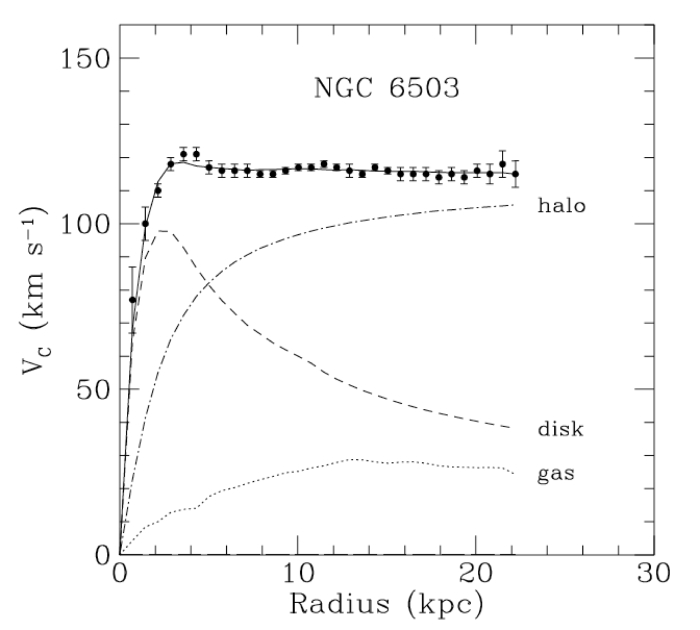
\includegraphics[width=0.4\linewidth]{plots/DarkMatter/RotationCurve_NGC6503.png}
\caption[The rotation curve of galaxy NGC~6503]{The measured rotation curve of the galaxy NGC~6503 from Ref.~\cite{RotationCurves_Begeman}, also showing the rotational-velocity profiles for the individual components of gas, stars, and the dark matter halo.}
\label{figRotationCurve}
%\end{figure}
\end{floatingfigure}

\begin{equation}
\label{eqVirialMass}
M_{\mathrm{tot}} \simeq \frac{2 \cdot R_{\mathrm{tot}} \cdot v^{2}}{G}.
\end{equation}

The amount of luminous matter is indicated by the luminosity of the galaxies. The measurements showed a deficit of luminous matter with respect to the mass of the cluster, which indicates the presence of large quantities ($>$90\%) of invisible mass, which is is revealed only by its gravitational interaction. The initial observation has been confirmed by a survey of the virial masses for 89 galaxy clusters, indicating the average mass-to-light ratio of 230$-$250~\cite{VirialMasses}.

Another evidence for the presence of dark matter has been found at galactic scale in the analysis of {\it rotation curves} of stars and gas~\cite{RotationCurves_Rubin} in disk galaxies, by measuring the redshift as a function of the distance $R$ to the galactic center. The light from the stars can be used for this purpose, but a clearer measurement has been performed by observing the emission of neutral hydrogen~\cite{RotationCurves_Begeman}, as its cloud typically extends far beyond the visible disk of stars, and hence can probe a larger region than the stars themselves. Since the majority of the luminous mass is located at the galactic center, it was expected that the motion of stars can be predicted by Newtonian dynamics, and the circular velocity should scale as $R^{-1/2}$. However, this is not the case for most galaxies, as shown in Fig.~\ref{figRotationCurve} by an example of galaxy NGC~6503~\cite{RotationCurves_Begeman}. The rotation curves of spiral galaxies are flat, while the stellar density falls off exponentially at large radii and hence cannot account for the observation. 
This indicates the existence of non-luminous matter superimposed upon the luminous disk. The rotation of the galaxies can be explained by introducing a dark matter halo with a mass density proportional to $R^{-2}$. The sum of the contributions from the visible matter in the disk and from the hydrogen gas, and dark matter in the halo reproduces the observed rotation curve.

Further evidence for invisible matter on the scale of galactic clusters is the phenomenon of {\it gravitational lensing}~\cite{GravitationalLensing_Review}, where a galaxy cluster acts as a lens for the light emitted from a more distant galaxy with high surface brightness, bending it with its gravitational field (see Fig.~\ref{figGravitationalLensing}) and resulting in multiple images of the background galaxy. Measurements of the light deflection provide a possibility to determine the mass of the galaxy cluster. This value is then compared to the luminous mass, which is calculated based on the X-ray luminosity. The mass-to-light ratio measured with this method~\cite{GravitationalLensing_Observation} confirms the results of the velocity dispersion measurements, pointing at the presence of a large fraction of non-luminous non-baryonic matter (dark matter). Additionally, it indicates the existence of non-luminous, but baryonic, component in the form of X-ray emitting plasma, which exceeds the mass of luminous matter by a factor of $\sim$6~\cite{GravitationalLensing_XrayPlasma}.

One of the strongest evidences for the existence of dark matter has been obtained by observing collisions of galaxy clusters~\cite{GravitationalLensing_BulletCluster, GravitationalLensing_Abell, GravitationalLensing_MACS1, GravitationalLensing_MACS2}. The diffuse clouds of the hot X-ray emitting intracluster plasma and interact electromagnetically, slowing down in the collision process, while the stars simply pass by one another without large disturbance. Since conglomerations of dark matter experience only gravitational interactions, they will also pass through one another, and hence exhibit very different dynamics during the collision compared to the hot interstellar gas. An example of such collision for Bullet cluster (1E0657-558)~\cite{GravitationalLensing_BulletCluster} is shown in Fig.~\ref{figGravitationalLensing_2}. The extent of cluster plasma, determined from X-ray emission, is shown in pink, and the distribution of the mass of the cluster, measured by gravitational lensing, is indicated in blue. The clouds of hot gas (baryonic matter) have been stripped away from their parent clusters, while the dominant mass is laterally displaced from the baryonic matter, thus showing a discrepancy in the strength of the gravitational force, consistent with the expectation of collisionless dark matter.

%\begin{floatingfigure}[r]{0.3\textwidth}
\begin{figure}[!h]
\centering
\subfigure[]{
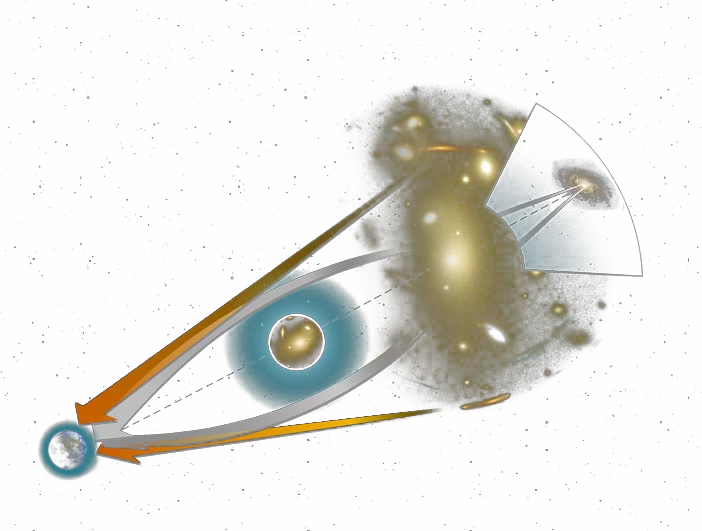
\includegraphics[height=0.325\linewidth]{plots/DarkMatter/GravitationalLensingNASA_white.png}
\label{figGravitationalLensing_1}}
\subfigure[]{
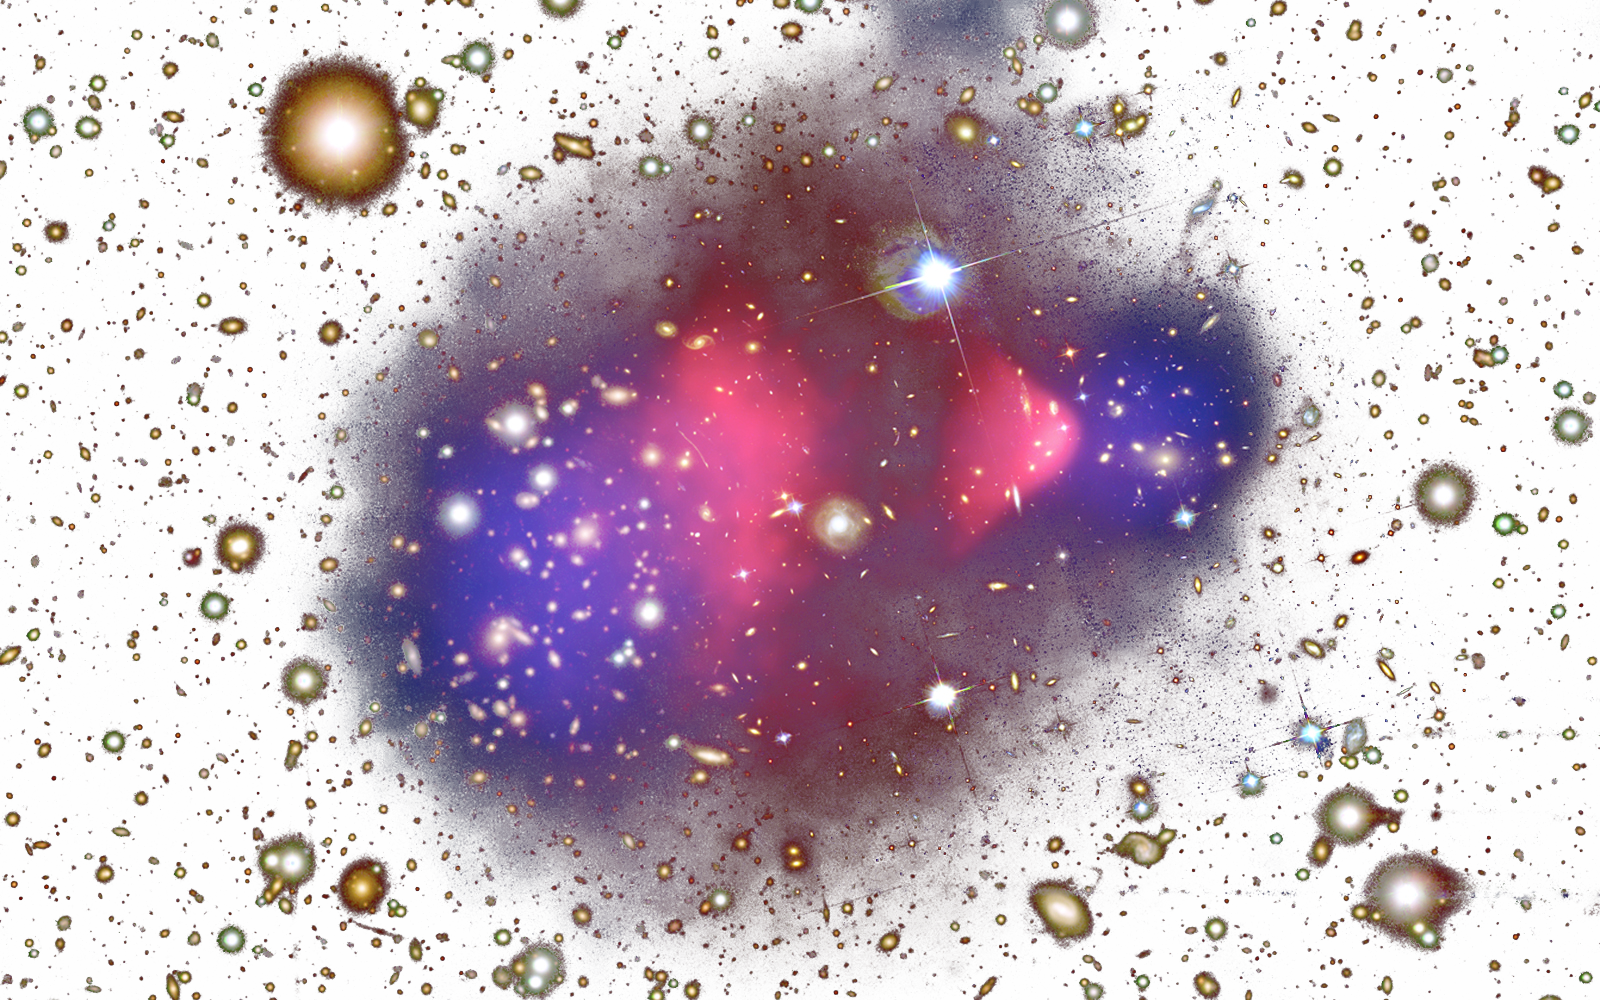
\includegraphics[height=0.325\linewidth]{plots/DarkMatter/BulletCluster_white.png}
\label{figGravitationalLensing_2}}
\caption[The gravitational lensing effect and the Bullet cluster with two colliding galaxy clusters]{(a) - the gravitational lensing effect: the galaxy cluster in the front acts as a strong gravitational lens for a distant galaxy behind with high surface brightness.  (b) - the Bullet cluster with two colliding galaxy clusters. The majority of the baryonic mass is located in the intracluster plasma, shown in pink, and the dominant cluster mass is shown in blue. Their displacement from one another can be explained by dark matter. Figures from Ref.~\cite{NASA}.}
\label{figGravitationalLensing}
\end{figure}
%\end{floatingfigure}

Evidence for dark matter on a universal scale is provided by the measurements of the cosmic microwave background (CMB), photons at microwave wavelengths, which exists as a consequence of the Big Bang. The temperature spectrum of CMB gives detailed information about the energy density at the time of photon decoupling. The data from Wilkinson Microwave Anisotropy Probe (WMAP)~\cite{WMAP_5year, WMAP_7year} has been used to measure the total matter and energy density in the universe ($\Omega_{tot}$ = 1.02$\pm$0.02), the total matter density ($\Omega_{m}$ = 0.266$\pm$0.029), and the density of baryonic matter ($\Omega_{b} = $0.0449$\pm$0.0028). This baryonic matter contributes only about 17\% of the matter density in the universe, and its density matches with the one from luminous mass measurements.

A standard cosmological model ($\Lambda$CDM) has been developed by combining the measurements of astrophysical systems at sizes ranging from galactic to universal scales. In this model, 4.6\% of the universe consists of atoms, the building blocks of stars and planets, 23\% is composed of non-baryonic dark matter that does not emit or absorb light, and so far is detected only indirectly by gravitational forces, as detailed above.  The remaining 72\% is an unknown component called dark energy that is responsible for the present-day acceleration of the expansion of the Universe~\cite{DarkEnergy}.

%On a universal scale 



%\section{Theoretical Predictions}
	\section{Theoretical Predictions}
\label{secTheoreticalPredictions}

One of non-baryonic particles that has a non-zero contribution to the matter density in the universe is the {\it neutrino}, which used to be considered an excellent candidate for non-baryonic dark matter~\cite{DM_neutrino}. 
There is a relic neutrino background in the Universe, left over from the Big Bang, similar to the photon CMB. Observation of atmospheric and solar neutrino oscillations have established that neutrino have a mass of $\geq$0.05~eV~\cite{NeutrinoMass_SuperK, NeutrinoMass_SNO}. Laboratory measurements of $\beta$-decay constrain the upper limit on neutrino mass to $<$2.05~eV (95\%~C.L.)~\cite{NeutrinoMass_Weinheimer}. This implies that the total relic density of neutrinos is $<$0.07~\cite{WMAP_5year}, thus they are not abundant enough to be the dominant component of dark mater. The neutrino component of dark matter is called `hot' dark matter: since they travel at relativistic speeds at the time of decoupling, they cannot reproduce the observed large structure in the Universe.

Another dark matter candidate are {\it axions}, light pseudo-scalar elementary particles postulated to resolve the strong CP problem in quantum chromodynamics (QCD)~\cite{CPviolation}. Axions are constrained to be very light, with a mass from 10$^{-6}$~eV to 10$^{-3}$~eV~\cite{AxionBounds}, and are expected to be extremely weakly interacting with ordinary matter, which assumes that they were not in thermal equilibrium in the early Universe. The axion relic density calculation relies on same production mechanism assumptions, which makes it possible to find an acceptable range where all constraints are satisfied. Hence, axions present a possible dark matter candidate~\cite{AxionsRosenberg}, and are being searched in experiments which stimulate the conversion of an axion into a single photon in magnetic field~\cite{AxionSearches}. 

While axions could be an excellent solution to the strong CP problem, their small mass requires that they are produced out of thermal equilibrium. In contrast, the dark matter candidates that originate as thermal relics (a process known as thermal freeze-out), can be explored. 
Shortly after the Big Bang, if production and annihilation rates for specific particles are equal, they are in thermal equilibrium with the rest of the Universe. Once the temperature of the Universe falls below the production threshold for this particle species, production ceases. Additionally, the annihilation rate is suppressed by the expansion of the Universe. The present mass density of particle $\chi$ in the units of particle density is given by~\cite{WIMPnucleusScattering1}:

\begin{equation}
\Omega_{\chi} h^{2} = \frac{m_{\chi} n_{\chi}}{\rho_{c}} \approx \frac{3\times10^{-27} \mathrm{cm^{3}s^{-1}}}{\sigma v}
\end{equation}
where $m_{\chi}$ is the particle mass, $n_{\chi}$ is the number density, $\rho_{c}$ is the critical density, $\sigma$ is the thermally averaged total annihilation cross section, and $v$ is the velocity. In order for $\Omega_{\chi}$ to have a value close to what we observe today, particle $\chi$ must have a very small cross section, on the level of weak interaction. 
As the cross section of dark matter interaction with ordinary matter is very small, and it must have a large mass to account for the gravitational effect, it is usually called {\it weakly interacting massive particles} (WIMPs). These hypothetical particles have masses from 1~GeV to 10~TeV.

Despite the standard model of particle physics is a fully renormalizable quantum field theory, it is clearly incomplete, as it has many open questions. In particular, it does not explain the dark matter observed in the Universe (see Section~\ref{secObservationalEvidence}). This problem could be solved by an introduction of new stable particle at the weak scale. One of the best motivated WIMP candidate is the {\it neutralino}, which emerges in the framework of supersymmetry (SUSY) theories, the extension of the standard model of physics unifying the four fundamental forces of nature (electromagnetic, weak, and strong nuclear interactions), which mediate the dynamics of the known subatomic particles. Neutralino is the lightest supersymmetric particle (LSP), stable in supersymmetric models where R-parity is conserved~\cite{LSP}, such as minimal supersymmetric extension to standard model (MSSM)~\cite{MSSM} or minimal supergravity (mSUGRA) theory ~\cite{SUGRA}. The theoretical predictions for WIMP mass and spin-independent WIMP-nucleon scattering cross section are shown in Fig.~\ref{figCMSSMparameterSpace}.

%\begin{floatingfigure}[r]{0.3\textwidth}
\begin{figure}[!h]
\centering
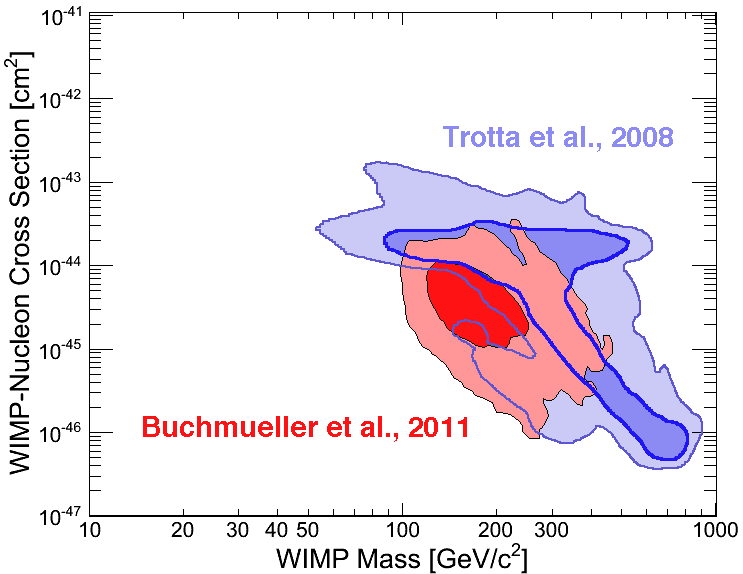
\includegraphics[width=0.475\linewidth]{plots/DarkMatter/wimp_expectation_modWithLabels.png}
\caption[The theoretical predictions for WIMP mass and spin-independent WIMP-nucleon scattering cross section with CMSSM]{The theoretical predictions for WIMP mass and spin-independent WIMP-nucleon scattering cross section with  constrained minimal supersymmetric extension to standard model (CMSSM)~\cite{LHC, Trotta}. Figure from Ref.~\cite{Marc}.}
\label{figCMSSMparameterSpace}
\end{figure}
%\end{floatingfigure}

%As time progresses, these rates begin to differ, the nature of which depends upon the particle�s annihilation cross section and mass. Once the temperature of the universe falls below the production threshold of this species, production ceases. Additionally, the expansion of the universe suppresses the annihilation rate; if this rate drops below the expansion rate then annihilation ceases as well, and a relic density of this particle will remain. The relic density of particle $\Chi$ depends upon is the thermally averaged
%total annihilation cross section multiplied by the velocity [$\sigma v$] as [29]:

%where mX , is the WIMP mass, nX is the number density, and ??v? is the thermally averaged
%total annihilation cross section multiplied by the velocity. In order for �X to have a value
%close to what we observe today, X must have a weak cross section [30], which already rules out most of the particles in the Standard Model.


%\section{Particle Dark Matter Searches}
%\label{secParticleDMsearches}
	\section{Dark Matter Searches}
\label{secParticleDMsearches}

The two main goals of the dark matter search are to demonstrate that galaxies are made of a new form of matter, which is the aim of direct and indirect detection techniques used by astroparticle physics community,  and to study the properties of this form of matter, such as their mass, lifetime, and coupling, in experiments at high energy particle colliders. 


%\subsection{Production in Colliders}
	\subsection{Production in Colliders}
\label{secProductionInColliders}

High energy particle accelerators, such as the Large Hadron Collider (LHC) or the Tevatron, might be able to produce WIMPs and to find dark matter~\cite{Colliders_1, Colliders_3}. The main advantages of collider searches are sensitivity to low dark matter masses, and that they do not suffer from astrophysical uncertainties.

Phenomenological consequence of R-parity is that supersymmetric particles can only be produced in colliders in pairs in the collision of ordinary matter. 
Since WIMPs are stable on the order of the lifetime of the Universe, they do not decay within the detector volume. 
Hence, dark matter candidates appear as `missing energy'~\cite{Colliders_1}. 

A typical collision involves quarks and gluons carrying only a small fraction of the parent energy, which implies that cross sections fall dramatically with the mass of produced states. Hence, light states can be produced with large rates, and constraints fall off for WIMP masses exceeding the typical energy reach of the colliders. The collider sensitivity to spin-dependent interactions is stronger than that of direct searches over a significant portion of parameters space, especially for light WIMP masses, where sensitivity of direct detection experiments is limited by energy thresholds~\cite{Colliders_3}.  However, while collider searches can constrain WIMP mass quite well, they do not have high sensitivity for its scattering cross section. Hence, dark matter searches at high energy particle colliders must be complemented by direct and indirect detection experiments. 
In addition, even if a WIMP is discovered in a collider, the existence of the galactic dark matter halo will still have to be proven.


% Indeed, for many operators, the direct detection rates are expected to be very small because of the velocity suppression, and colliders become the only way to effectively probe WIMP-hadron interactions. In the case of a WIMP whose dominant recoil is through a spin-dependent interaction, collider constraints are already much stronger even than the expected reaches of near-future direct detection experiments. Thus, if such an experiment were to observe a positive signal, the collider constraints would immediately imply a break- down of the effective field theory at collider energies, revealing the existence of a light mediator particle.


%\subsection{Indirect Detection}
	\subsection{Indirect Detection}
\label{secIndirectDetection}

Particle dark matter can be detected indirectly, by observing radiation produced in its annihilation reactions: $\gamma$-ray, synchrotron radiation, neutrino, positron and anti-proton fluxes~\cite{BertoneHooper}. Since the flux is proportional to annihilation rate, which depends on the square of the dark matter density, it is commonly searched in the regions where dark matter densities are expected to accumulate through inelastic collisions, such as the galactic center in the Sun or in dwarf galaxies.

High energy $\gamma$-rays, in the GeV$-$TeV energy range relevant for dark matter searches, can be directly detected only by space telescopes, since $\gamma$-rays will interact with matter via production of electron-positron pairs, with an interaction length much shorter than the thickness of the atmosphere~\cite{IndirectDetection_gamma}. The Energetic Gamma-Ray Experiment Telescope (EGRET) was one of four detectors on the Compton Gamma Ray Observatory (CGRO), which measured a diffused $\gamma$-emission from the galactic plane and discovered an excess above $\sim$1~GeV~\cite{Indirectdetection_EGRETexcess}. From the spectral shape, a WIMP mass of 50$-$100~GeV has been estimated~\cite{IndirectDetection_EGRETinterpretation}, which, however, has been ruled out by measurements of the anti-proton flux, and the observation might  be due to an inaccurate estimation of the detector sensitivity~\cite{IndirectDetection_EGRETexplanation}. The next generation Fermi Large Area Telescope (LAT, former GLAST) has been launched into orbit and is currently taking data~\cite{IndirectDetection_Fermi}.

On the ground, $\gamma$-rays can be indirectly detected with air shower detectors, observing the night sky for Cerenkov light emitted from charged particles produced in high energy $\gamma$-interactions in the upper atmosphere. These detectors, called Imaging Atmospheric Cerenkov Telescopes (IACTs), are sensitive in the energy range from $\sim$100~GeV to several TeV, and examine the $\sim$10~km high region, where the showers reach their maximum intensity. Examples of experiments are HESS~\cite{IndirectDetection_HESS} and MAGIC~\cite{IndirectDetection_MAGIC}, while the next-generation ground-based $\gamma$-ray observatory, the Cerenkov Telescope Array (CTA), is already being designed~\cite{IndirectDetection_CTA}.

WIMPs can annihilate in the core of the Sun or the Earth into muon neutrinos, which can escape and produce ultra-relativistic muons in charged current interactions with nuclei in terrestrial targets. They can be detected in large water- or ice-based neutrino telescopes. The most stringent bounds on high energy neutrinos from the Sun and the Earth come from the Super-Kamiokande~\cite{IndirectDetection_SuperK} experiment, AMANDA~\cite{IndirectDetection_AMANDA}, and its successor IceCube~\cite{IndirectDetection_IceCube}.

A cosmic anti-matter experiment, the satellite-borne charged cosmic ray detector PAMELA, has reported an excess of anti-protons~\cite{IndirectDetection_PAMELA1}, which may indicate annihilation of dark matter in the galactic halo, or may be caused by the production of positrons by near-by pulsars~\cite{IndirectDetection_PAMELA2}. 
	
%\subsection{Direct Detection}
	\subsection{Direct Detection}
\label{DirectDetection}

Direct detection of particle dark matter is possible via their interactions with nuclei in low background terrestrial targets, which appears as one of the most promising techniques. A WIMP elastically scatters off a nucleus in the target material, causing it to recoil and produces an energy deposition of $<$50~keV, which can be transformed into a measurable signal, such as scintillation light, charge, or heat (Fig.~\ref{figDetectionSignals}).

\begin{figure}[!h]
\centering
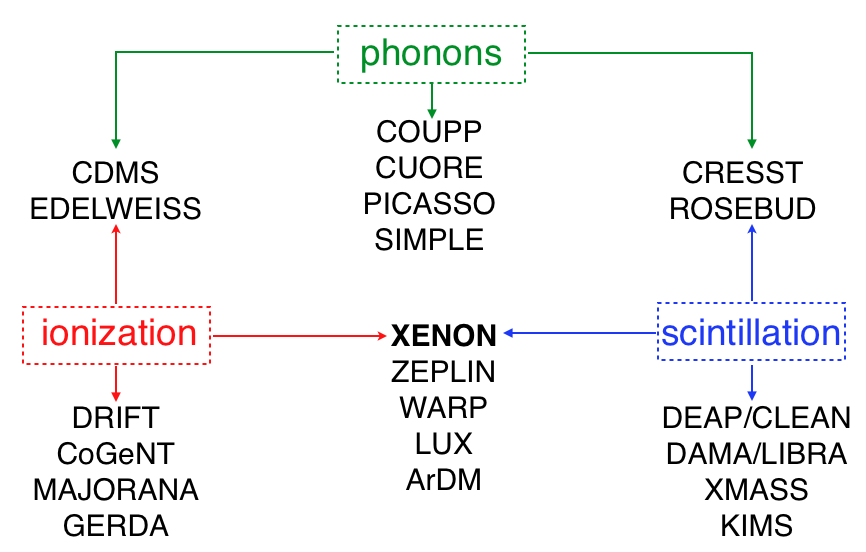
\includegraphics[width=0.6\linewidth]{plots/DarkMatter/DetectionSignals2.png}
\caption[Measurable signals from a WIMP interaction and chart of experiments for direct dark matter detection categorized by measurement technique]{Measurable signals from particle interactions and chart of experiments for direct dark matter detection categorized by measurement technique. The XENON experiment simultaneously measures scintillation and ionization signals, which allows to distinguish between electronic recoil (background) and nuclear recoils (signal) based on their ratio.}
\label{figDetectionSignals}
\end{figure}

The expected exponential nuclear recoil spectrum is featureless, and the shape depends on the mass of the WIMP and the target nucleus. The expected event rate $R$ can be evaluated by taking into account the density and the velocity distributions of WIMPs in the solar neighborhood, and the WIMP-nucleon cross section~\cite{BertoneHooper}:

\begin{equation}
R \approx \sum_{i} N_{i} \cdot n_{\chi} \cdot \sigma_{i\chi},\  \ \text{with}\ \  N_{i} = \frac{m}{A_{i}}\ \ \text{and}\ \ n_{\chi} = \frac{\rho_{\chi}}{M_{\chi}},
\end{equation}
where 
$i$ - index over all nuclei species in the detector, 
$N_{i}$ - number of target nuclei in the detector, 
$m$ - detector mass, 
$A_{i}$ - atomic mass of species $i$, 
$n_{\chi}$ - local WIMP density, 
$\rho_{\chi}$ - WIMP energy density, 
$\sigma_{\chi}$ - the cross section for the WIMP scattering off nuclei of species $i$, averaged over the relative WIMP velocity with respect to the detector.

Results for direct WIMP detection are usually obtained under simplifying assumptions on the galactic dark matter profile, assuming an isothermal profile with a flat rotation curve, a local density of 0.3~GeV/cm$^{2}$, and a Maxwell-Boltzmann velocity distribution. The uncertainties in the parameters lead to an enlargement of the allowed region in the WIMP mass $-$ cross section plane.

The Earth's motion around the Sun results in an annual modulation of the WIMP flux in the order of $<$10\%, thus modulation of the differential event rate over the course of the year, which can be used to separate the (modulated) WIMP signature from an (unmodulated) background. The Earth's speed relative to the galactic rest frame is largest in summer, hence, the WIMP flux with high speeds relative to the detector rest frame is largest in summer~\cite{EarthVelocitySpergel}. Therefore, for larger recoil energies a peak is expected roughly at the beginning of June, and for smaller recoil energies in winter~\cite{ModulationSignal}.

%Also possible is the inelastic WIMP scattering off nuclei~\cite{InelasticScattering_Goodman}, in which the WIMP interacts with orbital electrons, exciting or ionizing them, or with the target nuclei, leaving it in an excited state.
%This signature of this process is a nuclear recoil followed by the emission of a photon. However, the cross section to populate the excited state is a few orders magnitude below the elastic scattering because of phase space effects and smaller overlap of the wave functions~\cite{InelasticScattering_Ellis}. Thus, the backgrounds from natural radioactivity are strong competitors for such signature, and it is rarely used in the direct dark matter detection~\cite{InelasticScattering_DAMA}.

Basic requirements for direct detection detectors are a large target mass, low background, and low energy threshold. For the studies of spin-independent (scalar) coupling, heavy atoms are preferred as target material, as the corresponding cross section increases with the mass of the target nuclei. For spin-dependent (axial-vector) interactions, where the WIMP is expected to couple to unpaired nuclear spins $J$, using heavy targets is no advantage, as the cross section is proportional to $J\cdot$($J$+1) rather than to the number of nuclei, thus increases proportionally to the number of odd-even or even-odd isotopes. 

The first limits on WIMP-nucleon cross-sections have been obtained by the germanium-based double beta decay experiments, such as IGEX and the Heidelberg-Moscow experiment~\cite{FirstLimits_1, FirstLimits_2}, which excluded the first WIMP candidates, such as a heavy Dirac neutrino~\cite{DiracNeutrino} and cosmions~\cite{FirstLimits_Cosmions}. Low energy threshold and high energy resolution make germanium crystals a good target for dark matter searches using the ionization signal~(Fig.~\ref{figDetectionSignals}). 
An example of such an experiment is CoGeNT, which reported a signal~\cite{CoGeNT_LightWIMP} with a modulation~\cite{CoGeNT_modulation}. It could be explained by a WIMP in the mass range below $\sim$10~GeV. However, this explanation has been questioned by Ref.~\cite{Schwetz} and is in conflict with results of other experiments. Other current experiments of this type are GERDA~\cite{GERDA} and MAJORANA~\cite{MAJORANA}. 
However, their primary task is search for the neutrinoless double beta decay of the $^{76}$Ge isotope, a second-order weak process, whose discovery is the only practical way to determine if the neutrino is a Majorana particle~\cite{DoubleBetaGe76}.

Solid scintillation detectors are also being used for dark matter searches by means of light detection. In particular, DAMA is operating a detector based on radio-pure NaI modules, and displayed the annual modulation at a high significance level in the single-hit residual rate which could be due to low mass WIMPs interactions~\cite{DAMA}. Again, this is in conflict with the null-results of other experiments.

The COUPP experiment searches for WIMPs with a bubble chamber, operating a bulk superheated fluid  below the threshold for sensitivity to minimum ionizing particles, and distinguishes electronic and nuclear recoils with a very high efficiency by capturing stereoscopic bubble images and measuring the acoustic signals from bubble nucleation~\cite{COUPP}. PICASSO~\cite{PICASSO} and SIMPLE~\cite{SIMPLE} are examples of superheated droplets detectors, where micro-droplets are suspended in a matrix, which helps to avoid spontaneous bubble formation at the edges.

Some experiments operate at millikelvin temperatures and measure the energy by the collection of phonons simultaneously with the scintillation light, which provides discrimination between nuclear and electronic recoils. One of these experiments is CRESST~\cite{CRESST}, which utilizes Ca$_{2}$WO$_{4}$ crystals with silicon wafers and tungsten superconducting phase transition  thermometers. 
Other experiments, such as CDMS~\cite{CDMS_limit} and EDELWEISS~\cite{EDELWEISS_limit} achieve electronic recoil discrimination by measuring phonons and ionization in germanium crystals.

%The DRIFT experiment is based on the multiwire low pressure gaseous (CS$_{2}$) negative ion time projection chamber, which provides a possibility to reconstruct the ion tracks and deduce the directionality of a WIMP interaction~\cite{DRIFT}.

A very promising technology for WIMP detection are detectors based on noble elements. They are relatively inexpensive, provide easy scalability, require relatively simple cryogenic systems, and have high scintillation and charge yields. XMASS is one of current experiments with the largest target mass ($\sim$800~kg of liquid xenon)~\cite{XMASS}. However, it is a single phase spherical detector, which relies on background reduction only due to good position reconstruction and self-shielding, using only innermost $\sim$100~kg target for dark matter search. In double phase detectors, such as argon based WARP~\cite{WARP} and ArDM~\cite{ArDM}, and xenon-based ZEPLIN~\cite{ZEPLIN} and XENON~\cite{xe100-instrument, EMBG, xe100-run07, xe100-run08}, both scintillation and ionization signals are produced and detected, which allows for background discrimination with a high efficiency. The XENON100 dark matter search detector is the main topic of this thesis, and is covered in detail in the following chapters.



%The first evidence for a positive WIMP signal has been reported by the DAMA experiment in 1997~\cite{DAMA_1997}. However, this result has not been confirmed by 


%The scalar cross-section for spin-independent WIMP-nucleus scattering is given by the following equation~\cite{WIMPnucleusScattering1, WIMPnucleusScattering2}:

%\begin{equation}
%\sigma = F(Q) \frac{4m^{2}_{r}}{\pi} (Z f_{p} + (A-Z) f_{n})^{2},
%\end{equation}
%where $Z$ and $A-Z$ are number of protons and neutrons in the target nucleus, respectively; $f_{p}$ and $f_{n}$ is the WIMP coupling to protons and neutrons; $F(Q)$ - nuclear form factor; $m_{r}$ - reduced mass of the nucleon. 
%Thus, the scattering cross section scales approximately as $A^{2}$, and this gives an advantage of using xenon for WIMP-detection due to the size of the nucleus.


%\chapter{The XENON100 Detector}
	\chapter{The XENON100 Detector}
\label{chXe100detector}

The XENON100 detector, which is installed in the Laboratori Nazionali del Gran Sasso (LNGS), Italy, is the second generation detector within the XENON program, dedicated to the direct detection of dark matter in the form of WIMPs. It is a dual phase time-projection chamber (TPC), providing information about the 3D vertex of particle interactions. Being the successor of XENON10~\cite{xe10-instrument}, which has set some of the best limits on WIMP-nucleon scattering cross sections~\cite{xe10-independent, xe10-dependent}, XENON100 aims to improve this sensitivity by an increase of the target mass and a significant reduction of the background in the target volume, and by using an innovative design with a careful selection of the construction materials.

%\section{Detection Principle}
	\section{Detection Principle}
\label{secDetectionPrinciple}

A schematic description of a particle detection in a double phase xenon detector is shown in Fig.~\ref{figDetectionPrinciple}. When a particle interacts with a xenon atom, the energy transfer is split between ionization, excitation and heat~\cite{ScintillationProcesses1, ScintillationProcesses2, ScintillationProcesses3}. An excited xenon atom combines with another atom and produces an excited diatomic molecule~(\ref{eqScint1}). In the subsequent de-excitation it releases a photon with a wavelength of 178~nm, in the vacuum ultra-violet (VUV) region~(\ref{eqScint2}). Some of  electron-ion pairs produced by ionization recombine in the absence of an electric field~(\ref{eqScint4}), and VUV photons are also emitted through an excimer~(\ref{eqScint6}) when it decays back to the ground state~(\ref{eqScint7}).  Some of the energy is deposited in a non-radiative transition~(\ref{eqScint5}). 
%The following two processes of excitons $R^{*}$ and ions $R^{+}$ contribute to scintillation~\cite{ScintillationProcesses}:

\begin{floatingfigure}[l]{0.495\textwidth}
%\begin{figure}[!h]
\centering
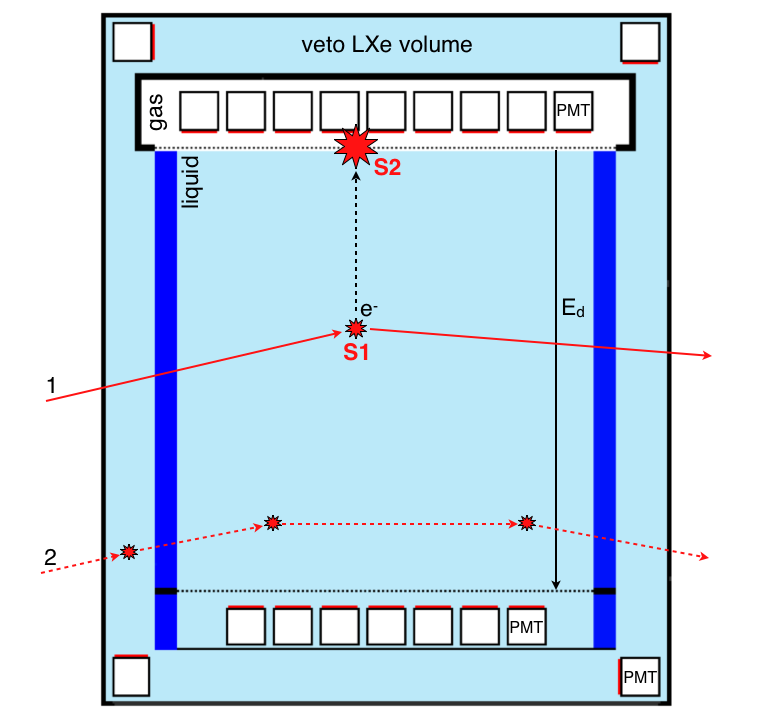
\includegraphics[width=0.495\linewidth]{plots/DetectionPrinciple/DetectionPrincipleWithLabels.png}
\caption[Particle detection principle with a double phase TPC]{Particle detection principle with a double phase TPC: 1 - valid signal event; 2 - multiple scattering event with an interaction in the liquid xenon veto volume.}
\label{figDetectionPrinciple}
%\end{figure}
\end{floatingfigure}

\begin{equation}
\label{eqScint1}
\text{Xe}^{*} + \text{Xe} \rightarrow \text{Xe}^{*}_{2},
\end{equation}
\begin{equation}
\label{eqScint2}
\text{Xe}_{2}^{*} \rightarrow 2\text{Xe} + h\nu
\end{equation}

\begin{equation}
\label{eqScint3}
\text{Xe}^{+} + \text{Xe} \rightarrow \text{Xe}^{+}_{2},
\end{equation}
\begin{equation}
\label{eqScint4}
\text{Xe}^{+}_{2} + e^{-} \rightarrow \text{Xe}^{**} + \text{Xe},
\end{equation}
\begin{equation}
\label{eqScint5}
\text{Xe}^{**} \rightarrow \text{Xe}^{*} + \text{heat},
\end{equation}
\begin{equation}
\label{eqScint6}
\text{Xe}^{*} + \text{Xe} \rightarrow \text{Xe}^{*}_{2},
\end{equation}
\begin{equation}
\label{eqScint7}
\text{Xe}^{*}_{2} \rightarrow 2\text{Xe} + h\nu
\end{equation}

The scintillation light has two components with different decay time constants (4~ns and 21~ns), corresponding to the decay of the singlet or triplet states of the excited dimer  Xe$^{*}_{2}$~\cite{SingletTriplet, SingletTriplet_dEdx}. For relativistic electrons, only one decay component with 45~ns decay time has been observed~\cite{SingletTriplet}. The pulse shapes are correlated with $dE/dx$, thus differ for particles of different type. This provides a mechanism for pulse shape discrimination (PSD). However, statistical fluctuations of the pulse shape at low energies, and fluctuations in the photon time-of-flight in the detectors of relatively large size, such as XENON100, do not allow discrimination between electronic interactions from nuclear recoils with the required precision~\cite{XenonPSD}.

%The excitation (fast) component and recombination (slow) components of the scintillation have the time dependence~\cite{SlowFastComponents}:
%\begin{equation}
%\label{eqFastSlow1}
%A_{exc} = C_{0} \cdot e^{-t/\tau_{exc}}
%\end{equation}

%\begin{equation}
%\label{eqFastSlow2}
%A_{rec} = D_{0} \cdot \frac{1 - e^{t/\tau_{exc}}}{(1+ e^{t/\tau_{rec}})^{2}}
%\end{equation}

%The time constants are . For gamma interaction, 100\% of the light is emitted in a 

Xenon atoms do not absorb their own scintillation light, because the photons originate from the decay of the excimer state. This prompt initial scintillation light (S1) is detected by photomultiplier tubes (PMTs) on the top and bottom of the target volume. 
When an electric field is applied across the liquid xenon target, some of the ionization electrons are removed from the interaction site, do not recombine and can be detected independently from the S1 light signal. The electrons created by ionization are drifted and extracted into the gas phase above the liquid xenon target, and accelerated with a high electric field, producing an electro-luminescence signal (S2)~\cite{S2} via collisions with xenon atoms, which is detected by PMT arrays above and below the target volume. 

In the standard scenario, WIMPs are expected to elastically scatter off xenon nuclei resulting in low energy nuclear recoils (NR). Neutrons with energies in $\sim$MeV range passing through the detector also produce low energy nuclear recoils, whereas $\gamma$-rays and electrons produce electronic recoils (ER). 
Because of the different $dE/dx$, the energy deposition of NR and ER results in different probability of electron-ion pairs recombination (\ref{eqScint4}), and thus different ratios of the yield of scintillation light and ionization charge. The ratio of the primary (S1) and secondary (S2) scintillation signals provides a possibility to distinguish electronic interactions (background) from nuclear recoils (signal), and to reject the electromagnetic background. Using this discrimination technique, XENON10 and XENON100 reached an ER rejection efficiency better than 99\% at $\sim$50\% NR acceptance~\cite{xe10-independent, xe100-run07}.

In a homogeneous electric field, the position in the $XY$ plane at which the proportional scintillation occurs is correlated with that of the original interaction, and leads to a clustered hit pattern on the top PMT array. This is used to reconstruct the $X$ and $Y$ coordinates of an event, as described in Chapter~\ref{chPositionReconstruction}. 
In addition, the time difference between the S1 and S2 signals provides information about the $Z$ coordinate of the interaction. The 3D position reconstruction capability allows localization and rejection of the events at the edges of the target volume, thus significantly reducing the external gamma and neutron backgrounds~(see Chapters~\ref{chERbackground} and \ref{chNRbackground}).

If a particle has deposited energy at multiple places in the target, then two or more S2 pulses are recorded in the trace. Such an event is a multiple scatter event and is rejected in the analysis since the predicted behavior of the WIMP, due to its very low scattering cross-section, would produce only single scatters~(see Section~\ref{secDataQualityCuts}).

The liquid xenon target in the XENON100 detector is surrounded from all sides by a liquid xenon layer, equipped with PMTs and acting as an active veto. Events that have a coincident signal in the veto (illustrated in Fig.~\ref{figDetectionPrinciple}) are removed from the analysis, which provides a significant reduction of background due to $\gamma$-interactions (see Section~\ref{secDetectorMaterials}).


%to exploit the self-shielding capability of liquid xenon due to its high 


	\section{Detector and Shield Design}
\label{secDetectorDesign}

A total amount of 161~kg of LXe is enclosed in the vacuum insulated cryostat, made from the low activity stainless steel of type 1.4571/316Ti (316Ti SS). The target consists of 62~kg of LXe, defined by a structure made from polytetrafluoroethylene (PTFE, {\it Teflon}) and copper.
The target volume is viewed by two arrays of photomultiplier tubes (PMT), one on the bottom immersed in LXe, and one in the gas phase above the target volume.
The electric fields of the TPC are generated by applying potential differences across the electrodes, which are made of stainless steel meshes welded onto 316Ti SS rings. They include two electrodes on the bottom of the TPC above the bottom PMT array, and a stack of three electrodes around the liquid-gas interface.

The passive shield is shown in Fig.~\ref{figXe100shield_1}. It encloses the detector in 4$\pi$, and is installed on a 25~cm slab of polyethylene. From outside to inside, it consists of tanks filled with water (thickness 20~cm, Fig.~\ref{figXe100shield_2}) to shield against ambient neutrons, placed on three sides and on top of the shield. After the water shield, there are two layers of lead: a 15~cm outer layer and a 5~cm inner layer, which has a low contamination of the radioactive isotope ${^{210}}$Pb (Section~\ref{secDetectorMaterials}). Inside the lead, there are 20~cm of polyethylene to shield against further neutron backgrounds. The innermost shield layer consists of 5~cm thick (0.5~cm on the bottom) copper plates. It reduces the gamma background from the outer shield layers. The inner shield cavity is constantly purged with high purity boil-off nitrogen at a rate of $\sim$17~standard liters per minute (slpm) in order to avoid penetration of radon. Detector components with relatively high radioactive contamination are mounted outside of the shield, for example signal and high voltage feedthroughs, vacuum pumps, pressure sensors and associated electronics. An important detector design feature, which has contributed to the low background rate of XENON100, is `remote cooling' - the installation of the cryogenics system, based on a pulse tube refrigerator (PTR)~\cite{PTR}, outside the passive shield, far away from the xenon target.

\begin{figure}[!h]
\centering
\subfigure[]{
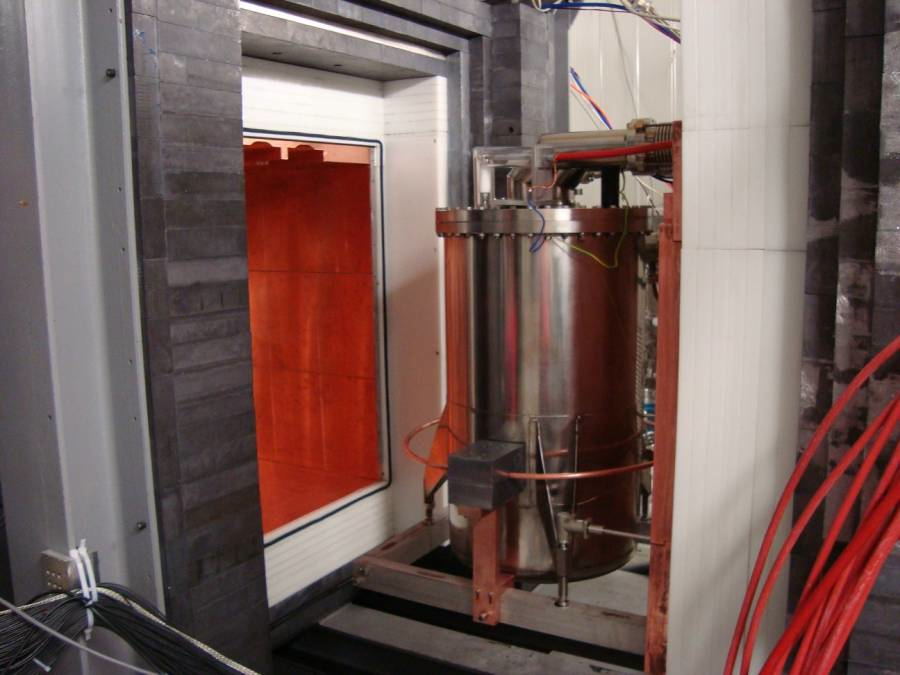
\includegraphics[height=0.45\linewidth]{plots/Detector/Xe100shield.png}
\label{figXe100shield_1}}
\subfigure[]{
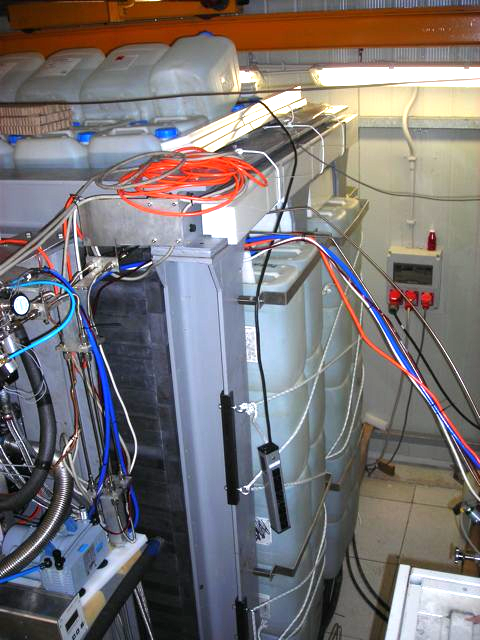
\includegraphics[height=0.45\linewidth]{plots/Detector/WaterShield.png}
\label{figXe100shield_2}}
\caption[The XENON100 detector with the open shield door, and the water shield]{The XENON100 detector with the open shield door (a), and the water shield (b).}
\label{figXe100shield}
\end{figure}

The schematic drawing of the XENON100 detector is shown in Fig.~\ref{figXe100CAD}.
The quasi-cylindrical TPC is formed by 24 interlocking PTFE panels with a thickness of 6.35~mm, see also Fig.~\ref{figTPC}. PTFE reflects scintillation light with high efficiency~\cite{yamashita}, and optically separates the 62~kg target volume from the surrounding liquid xenon, which is in average 4~cm thick and has a total mass of 99~kg. This allows exploitation of the self-shielding capability of liquid xenon due to its high density (2.83~g/cm$^{3}$ at T = 182~K, P = 2.3~atm) and high atomic number ($Z$ = 54). In addition, this volume around the target is instrumented with PMTs, becoming an active veto for background reduction by rejecting events in which a particle deposits part of its energy in the veto volume. 

\begin{figure}[!t]
\centering
%\includegraphics[width=1.0\linewidth]{plots/Detector/Xe100_CAD_withLabels2.png}
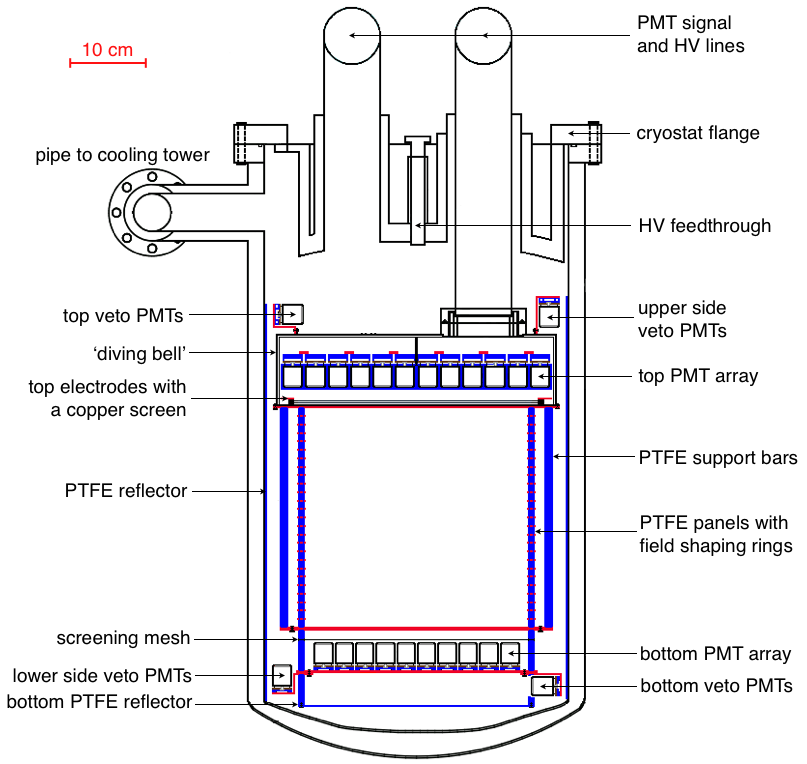
\includegraphics[width=1.0\linewidth]{plots/Detector/Xe100_CAD_withLabelsAndScale.png}
\caption[Schematic view of the XENON100 detector]{Schematic view of the XENON100 detector. The colors show: black - stainless steel, red - copper, blue - PTFE. Figure published in Ref.~\cite{xe100-instrument}.}
\label{figXe100CAD}
\end{figure}

\begin{table}[!t]
\centering
\caption[Thickness of the 316Ti stainless steel used for different detector components, and their weight]{Thickness of the 316Ti stainless steel used for different detector components, and their weight. The support rings for the top electrodes are milled down to 2.5~mm from 3.0~mm plates.}
\label{tabStainlessSteel}
\vspace{0.2cm}
\begin{tabular}{>{\footnotesize}l|>{\footnotesize}l|>{\footnotesize}c}
%\begin{tabular}{l|l|c}
\hline
Detector component 					& Steel thickness [mm]		& Weight [kg] \\
\hline
Inner cryostat vessel						& 1.5 					& 12.2 \\
Outer detector vessel					& 1.5						& 14.1 \\
Cryostat lid with the top pipes				& 1.5						& 30.8 \\	
Flange								& 25.0					& 12.8 \\
Diving bell							& 2.5						& 3.6 \\
Support ring for the cathode 				& 1.5						& 0.074 \\
Support ring for the screening mesh			& 3.0						& 0.156 \\
Three support rings for the top electrodes 	& 3.0 					& 0.24 \\
Cryostat support bars					& 25.0					& 49.68 \\
\hline
\end{tabular}
\end{table}

%The cryostat and some other parts of the detector are made from austenitic stainless steel of type 316Ti in AISI standard~\cite{316Ti}.
Steel plates of various thickness have been used for different detector components, with different radioactive contaminations (details in Section~\ref{secScreening}). The thickness of the 316Ti stainless steel and the corresponding weight of the detector components are shown in Table~\ref{tabStainlessSteel}. The total weight of the cryostat vessel is 70.0~kg, which is only 30\% of that of the XENON10 detector's cryostat~\cite{xe10-instrument}. 
The cryostat is supported inside the shield by 316Ti SS bars, which are mounted onto the movable shield door (Fig.~\ref{figXe100shield_1}). 

The inner vessel containing the LXe is lined on the walls and the bottom with a 1.5~mm thick PTFE layer  in order to increase the light collection efficiency in the active veto volume. The pipes guiding PMT signal and high voltage cables have been designed to be single wall to reduce the amount of radioactive material close to the detector.

Electrons created by ionization in the LXe target are drifted upwards by an electric field created by applying voltage on the cathode, a 75~$\mu$m thick stainless steel mesh with hexagonal structure with a 5~mm pitch, installed on the bottom of the TPC. The initial design has foreseen to use a high voltage of $-$30~kV to generate a drift field of 1~kV/cm. Electron field emission and subsequent scintillation in the strong electric field around the cathode wires resulted in induced single photoelectron-like events in the waveforms. As a result, the operation voltage has been lowered to $-$16~kV for stable operation, which corresponds to a drift field across the TPC of 0.53~kV/cm. In order to shield the bottom PMTs from this electric field, an additional grounded electrode (50~$\mu$m mesh) is installed below the cathode.

\begin{floatingfigure}[l]{0.45\textwidth}
%\begin{figure}[!h]
\centering
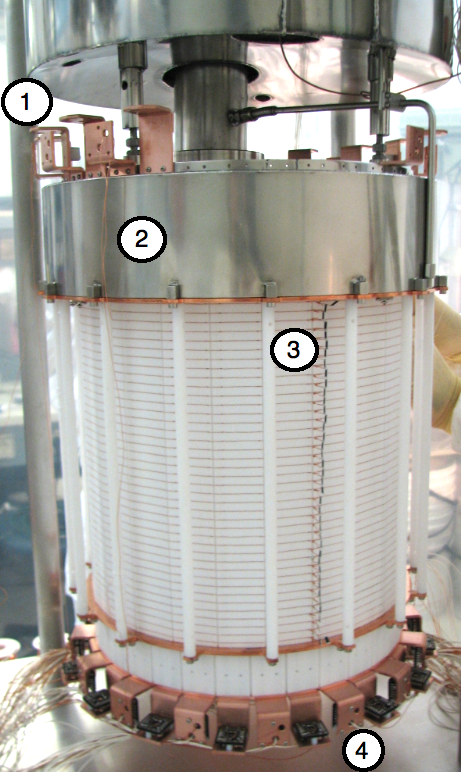
\includegraphics[height=0.65\linewidth]{plots/Detector/TPC_withLabels.png}
%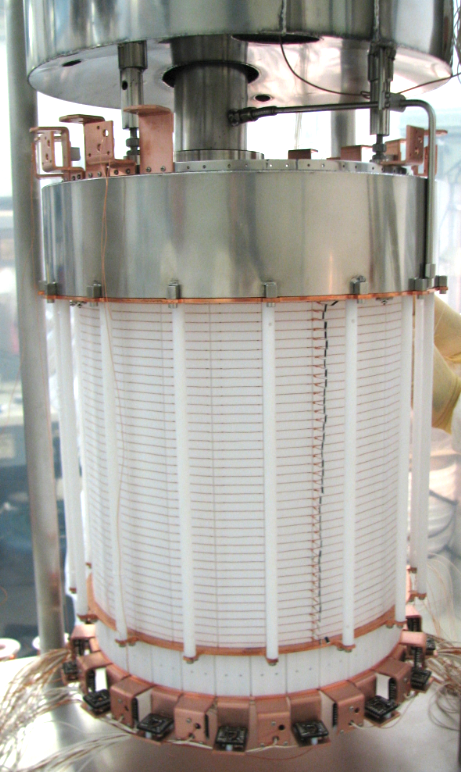
\includegraphics{plots/Detector/TPC.png}
\caption[The XENON100 time-projection chamber]{The XENON100 TPC during detector assembly in the clean room: 1- copper angles for the top and upper side veto PMTs, 2 - `diving bell', 3 - resistor chain connecting the field shaping rings, 4 - copper angles for the bottom and lower side veto PMTs.}
\label{figTPC}
%\end{figure}
\end{floatingfigure}

The gas phase for charge amplification via proportional scintillation is maintained using a `diving bell' system, made from 316Ti SS with a total weight 3.6~kg. It allows the liquid level to be kept constant at a precise height while having an additional layer of LXe above the TPC. A slight overpressure in the bell is provided by the gas returning from the continuous recirculation system.
The liquid level is adjusted by changing the recirculation rate, and by adjusting the height of the gas outlet from the bell by a motion feedthrough.

An extraction field is created across the liquid-gas interface by applying high voltage on the anode, 125~$\mu$m mesh with 2.5~mm pitch, which is placed inside the diving bell. The value of the extraction field depends on the position of the liquid-gas interface, which is adjusted to give $\sim$12~kV/cm in the gas phase at +4.5~kV applied to the anode. This field is high enough to obtain an extraction efficiency close to 100~\%~\cite{ExtractionField}. 
Two additional electrodes are installed below and above the anode and are kept at ground potential in order to close the field cage and shield the top PMT array from the high electric field.  The gaps between the top electrodes are 5~mm, and the liquid level is adjusted between the lower two of them. The entire stack of the top electrodes is optimized for optical transparency and minimal impact on the S2 resolution.

The scintillation light is detected by 242 one square inch R8520-06-AL Hamamatsu PMTs. They are among the PMTs with the lowest measured radioactivity (see Section~\ref{secScreening}), and are optimized for operation in LXe (at T = 182~K, P = 2.3~atm). 
The top PMT array consists of 98 PMTs in a PTFE support structure inside the diving bell, and 80 PMTs are installed below the cathode in the LXe. Additionally, 64 PMTs are mounted on copper angles and view liquid xenon of the veto volume.

%(milled from 3.0 SS plates)
%`

%\section{Gas Purification and Cryogenics}
	\section{Cryogenic System and Gas Purification}
\label{secGasSystem}

%The xenon gas for the XENON100 detector is stored in four high pressure aluminum cylinders, shown in Fig.~\ref{figGasRack}. They can be immersed in the dewars with $\sim$70~l capacity, and cooled down with liquid nitrogen, in order to recover xenon from the detector. 

%\begin{figure}[!h]
%\centering
%\subfigure[]{
%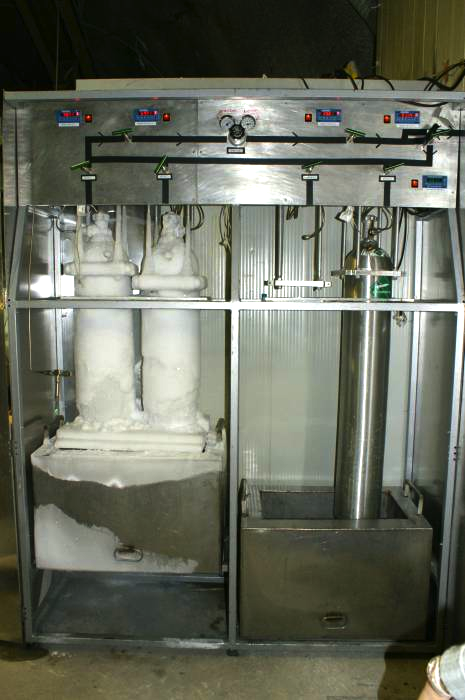
\includegraphics[height=0.5\linewidth]{plots/Detector/GasRack.png}
%\label{figGasRack_1}}
%\subfigure[]{
%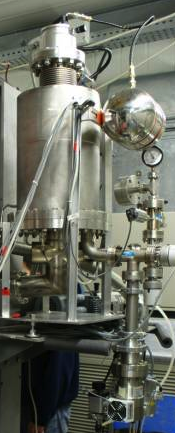
\includegraphics[height=0.5\linewidth]{plots/Detector/CoolingTower_door.png}
%\label{figGasRack_2}}
%\subfigure[]{
%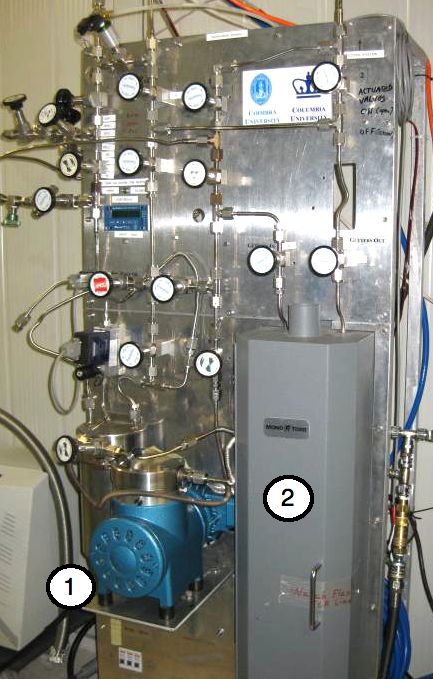
\includegraphics[height=0.5\linewidth]{plots/Detector/PurificationPanel_withLabels.png}
%\label{figGasRack_3}}
%\caption[The XENON100 gas system]{The XENON100 gas system. (a) - gas bottle rack during recuperation. (b) - cooling tower with a pulse-tube refrigerator (PTR) mounted on the shield door. (c) - gas recirculation and purification rack: 1 - recirculation pump, 2 - high temperature getter.}
%\label{figGasRack}
%\end{figure}


%\begin{floatingfigure}[lh]{0.3\textwidth}
%\begin{figure}[!h]
%\centering
%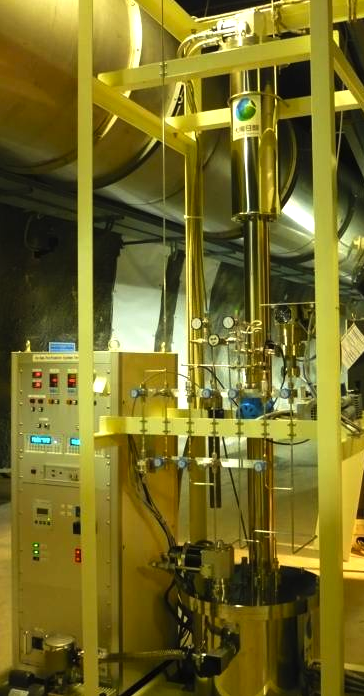
\includegraphics[height=0.6\linewidth]{plots/Detector/DistillationColumn.png}
%\caption{Cryogenic distillation column for krypton removal.}
%\label{figDistillationColumn}
%\end{figure}
%\end{floatingfigure}

%\begin{floatingfigure}[r]{0.3\textwidth}
%\begin{figure}[!h]
%\centering
%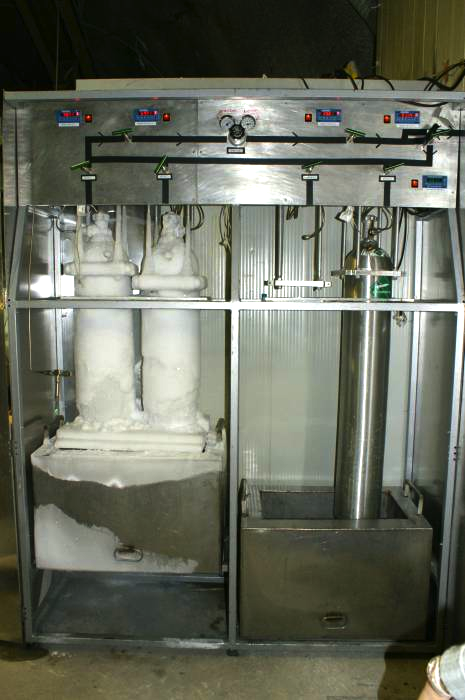
\includegraphics[width=0.3\linewidth]{plots/Detector/GasRack.png}
 %\caption{The XENON100 gas bottle rack during recuperation.}
%\label{figGasRack}
%\end{figure}
%\end{floatingfigure}

The schematic diagram of the cryogenic system of the XENON100 experiment is shown in Fig.~\ref{figCoolingTower_1}. It is based on Iwatani PC150~\cite{PTR} pulse tube refrigerator, powered by a 6.5~kW helium compressor. The measured cooling power is 200~W at 170~K, which allows the xenon gas to be liquified during the detector filling at a rate of $\sim$3~kg/hour.  The PTR is mounted together with its motor valve and buffer tank on a small double-walled vessel outside of the detector shield (Fig.~\ref{figCoolingTower_2}). The bottom of this vessel is connected to the detector cryostat with a vacuum insulated pipe, at a height above the liquid level. 
The PTR cold head is mounted on a cylindrical copper block, and then sealed to the inner vessel of the PTR cryostat with an aluminum wire, so that the PTR can be serviced or even replaced without exposing the detector volume to air. The temperature and pressure of the detector is regulated with an electric heater, which is installed in a copper cup connected to the cold head. The temperature is measured with Pt100 resistance thermometers connected to a PID controller.

When the gas from the detector reaches the cold head, it is liquefied, and the drops of liquid xenon are collected by a funnel and transferred via a 1/4-inch diameter pipe into the detector cryostat. The transfer is driven by gravity, therefore the connecting pipe is inclined by 5$^{\circ}$ to the horizontal.

\begin{figure}[!b]
\centering
\subfigure[]{
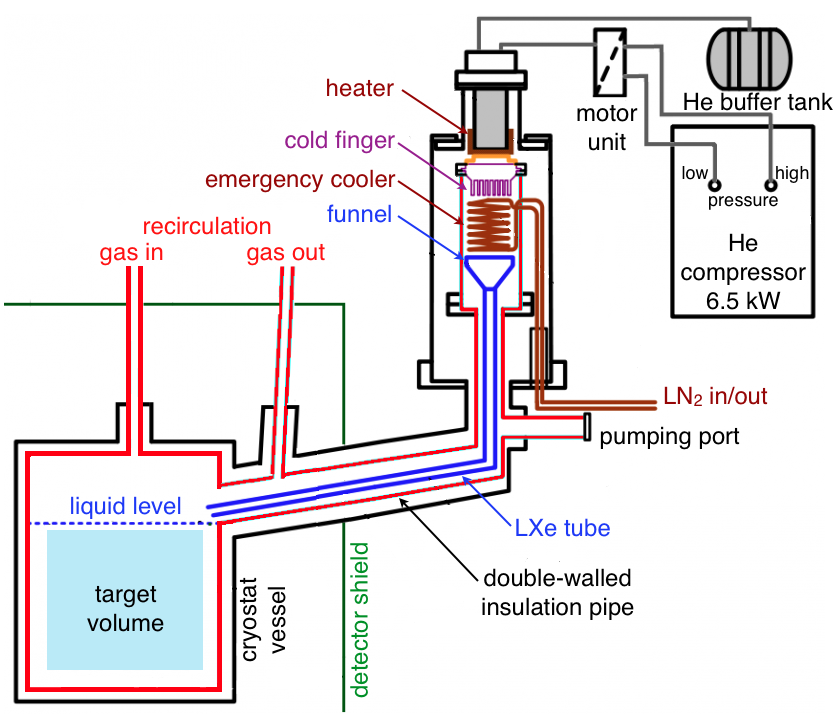
\includegraphics[height=0.6\linewidth]{plots/Detector/schemeMod_CoolingSystem.png}
\label{figCoolingTower_1}}
\subfigure[]{
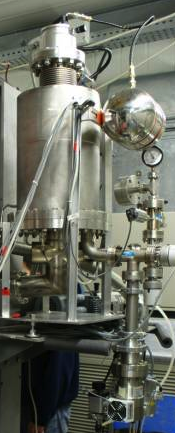
\includegraphics[height=0.6\linewidth]{plots/Detector/CoolingTower_door.png}
\label{figCoolingTower_2}}
\caption[The schematics of the XENON100 cryogenic system, and the cooling tower with pulse tube refrigerator]{The schematics of the XENON100 cryogenic system (a), and the cooling tower with pulse tube refrigerator (b). Scheme from Ref.~\cite{xe100-instrument}.}
\label{figCoolingTower}
\end{figure}

A copper coil, winded around the PTR cold head and connected to an external liquid nitrogen dewar, provides cooling in case of power outage, PTR failure, or when additional cooling power is needed in case of a loss of insulation vacuum. The external dewar is always kept full (above 80\%), and equipped with an actuated valve which is controlled via the detector pressure. This emergency system provides 48~hours of stable operation in case of a failure of the main cooling system.

Electro-negative impurities (such as oxygen) and water present in xenon gas affect the light and charge yields, respectively. In order to achieve the required electron lifetime and long VUV absorption length, their concentration has to be well below 1~parts-per-billion (ppb). The xenon purification is performed with a high temperature metal getter (MonoTorr~PS4-MT15-R-1~\cite{MonoTorr}). The continuous gas flow through the getter of 5~slpm is achieved by a diaphragm pump (KNF~N.143~\cite{KNFpump}). The gas recirculation system and its schematics are shown in Fig.~\ref{figPurificationPanel}. The xenon gas for the XENON100 detector is stored in four high pressure aluminum cylinders. In order to recover xenon from the detector, they are immersed in dewars with $\sim$70L capacity, and cooled with liquid nitrogen. 

\begin{figure}[!h]
\centering
\subfigure[]{
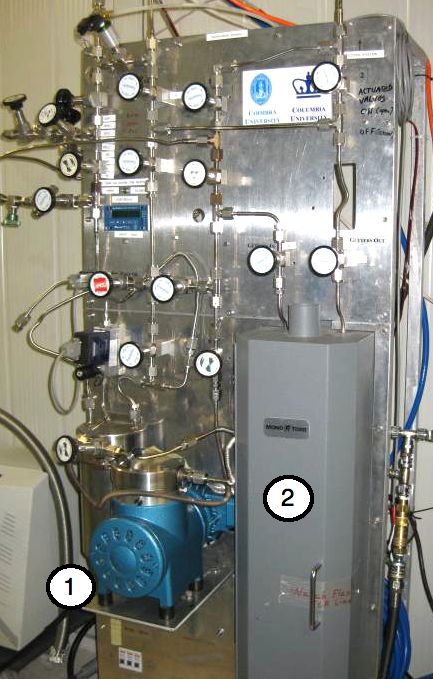
\includegraphics[height=0.55\linewidth]{plots/Detector/PurificationPanel_withLabels.png}
\label{figPurificationPanel_1}}
\subfigure[]{
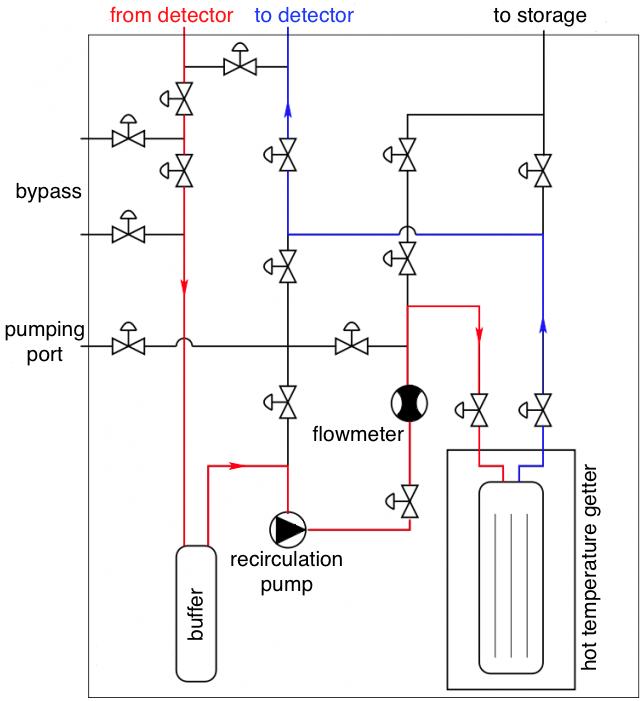
\includegraphics[height=0.55\linewidth]{plots/Detector/schemeMod_PurificationPanel.png}
\label{figPurificationPanel_2}}
\caption[The XENON100 gas purification panel]{The XENON100 gas purification panel: 1 - recirculation pump; 2 - hot getter. Scheme from Ref.~\cite{xe100-instrument}.}
\label{figPurificationPanel}
\end{figure}

Commercially available xenon gas has a concentration of krypton at the ppm level.
Natural krypton contains about 10$^{-11}$ of radioactive $^{85}$Kr~\cite{Kr85abundance_1, Kr85abundance_2}. 
The background from the beta decay of $^{85}$Kr, with half-life of 10.76~years and endpoint energy of 687~keV, is a potential limitation in the sensitivity of dark matter searches using xenon targets. 

\begin{figure}[!t]
\centering
\subfigure[]{
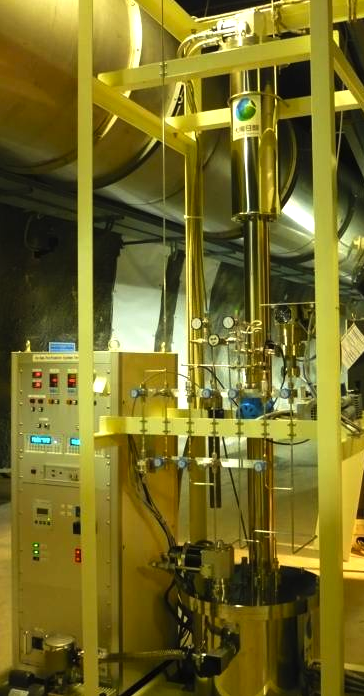
\includegraphics[height=0.6\linewidth]{plots/Detector/DistillationColumn.png}
\label{figDistillationColumn_1}}
\subfigure[]{
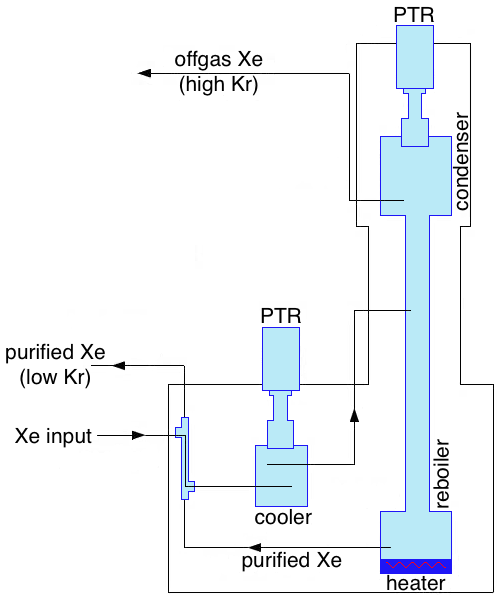
\includegraphics[height=0.6\linewidth]{plots/Detector/schemeMod_DistillationColumn.png}
\label{figDistillationColumn_2}}
\caption[Cryogenic distillation column for krypton removal]{Cryogenic distillation column for krypton removal. Scheme published in Ref.~\cite{xe100-instrument}.}
\label{figDistillationColumn}
\end{figure}

Krypton concentration in xenon can be reduced by distillation and adsorption-based chromatography methods. 
The gas used in the XENON100 experiment has been processed at a commercial distillation plant to reduce the concentration of krypton to $<$10~ppb, however, still above the XENON100 requirements of $\sim$100~parts-per-trillion (ppt) in order to reach the designed sensitivity.
The high-temperature getter used in the experiment to purify xenon from water and electronegative contaminants does not remove the noble gas krypton. Additional gas purification is achieved with a cryogenic distillation column based on the difference of the boiling points for krypton and xenon (120~K and 165~K at 1~atm, respectively). The krypton removal column has been developed by Taiyo Nippon Sanso~\cite{NipponSanso}, and is shown in Fig.~\ref{figDistillationColumn_1}. It is based on McCabe-Thiele method~\cite{McCabe} and is designed to deliver a factor of 1000 reduction of krypton concentration in a single pass. The schematic circuit is illustrated in Fig.~\ref{figDistillationColumn_2}. The main element in the distillation system is a tower in which liquid-gas equilibrium is maintained. A liquid is boiled using a heater in the `reboiler' vessel at the bottom of the tower. A condenser, placed on its top, maintains a constant temperature profile in the tower. The xenon gas is cooled down to a near boiling point and then supplied to a feed point. The processed xenon obtained from the reboiler contains a lower concentration of krypton than the original gas, and xenon with a higher krypton concentration is obtained at the top of the tower. 

The purification is performed in XENON100 with rate of $\sim$1.7~slpm, and the processing of the total amount of xenon required to fill the detector (161~kg) takes about two weeks, compared to 2-3~days needed for normal filling and recovering. The reduction of the krypton concentration down to a few ppt has been reported in Ref.~\cite{DistillationColumn}, where a small sample of processed xenon gas has been analyzed by mass spectrometry. This level of purity has not yet been achieved by XENON100 (see Section~\ref{secDelayedCoincidenceKr85}), however, this is the first large-scale experiment sensitive to such ultra-low krypton concentration.


%\section{Data Acquisition}
	\section{Electronics and Data Acquisition}
\label{secDAQ}

%\begin{floatingfigure}[l]{0.3\textwidth}
\begin{figure}[!t]
\centering
%\subfigure[]{
%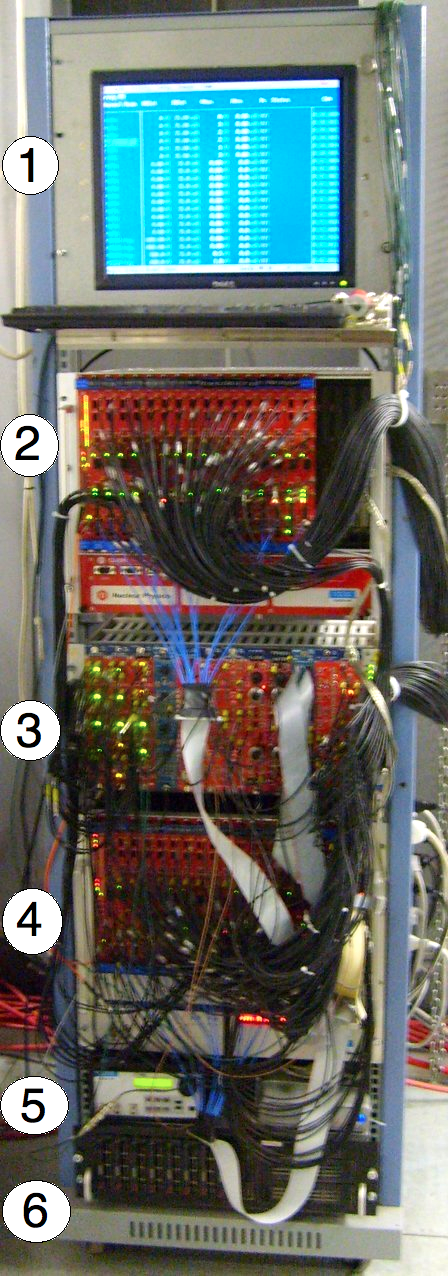
\includegraphics[height=0.5\linewidth]{plots/Detector/DAQ_withLabels.png}
%\label{figDAQ_1}}
%\subfigure[]{
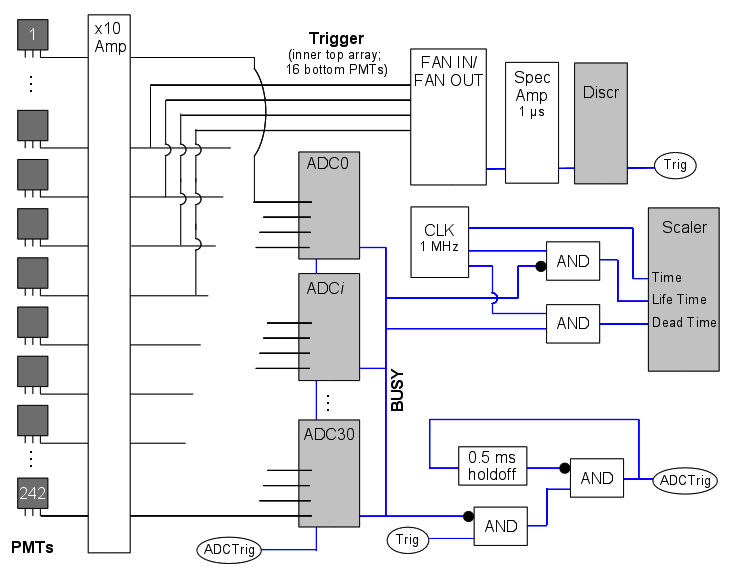
\includegraphics[width=0.9\linewidth]{plots/Detector/DAQschemeNew2.png}
%\label{figDAQ_2}}
%\caption[Schematics of the XENON100 data acquisition system]{SChematics of the XENON100 data acquisition system in the electronics rack: 1 - HV control panel; 2 and 4 - ADCs; 3 - clocks, FANs, discriminators, shaping amplifiers, gate generators,  scalers; 5 - LED pulser; 6 - storage disk. A scheme in Fig.~\ref{figDAQ_2} from Ref.~\cite{xe100-instrument}.}
\caption[Schematics of the XENON100 data acquisition system]{Schematics of the XENON100 data acquisition system. Figure from Ref.~\cite{xe100-instrument}.}
\label{figDAQ}
\end{figure}
%\end{floatingfigure}

\begin{figure}[!t]
\centering
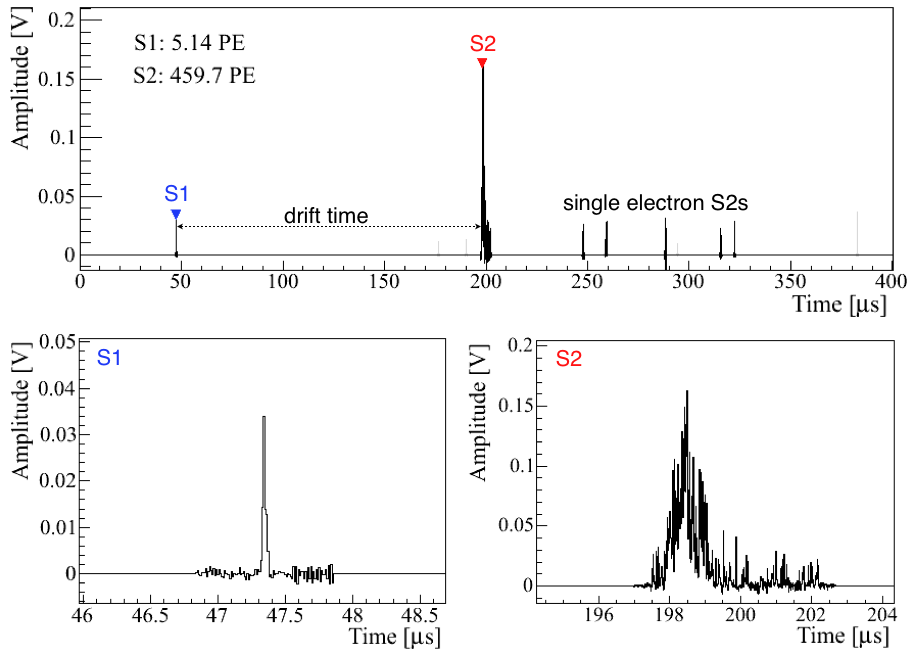
\includegraphics[width=0.9\linewidth]{plots/Detector/Waveform_withLabels.png}
\caption[A waveform of a low energy event in XENON100]{A waveform of a low energy event in XENON100. The bottom plots show a zoom into S1 and S2 peaks identified in the trace. The structures with the size of $<$40~PE after the main S2 peak are S2 signals from single electrons extracted into gas phase. Figure published in Ref.~\cite{xe100-instrument}.}
\label{figWaveform}
\end{figure}

The PMT signals are amplified by a factor 10 with Phillips PS776 amplifiers, and digitized with CAEN V1724 flash ADCs with 100~MHz sampling rate, 14~bit resolution, and 40~MHz bandwidth. The schematics of the XENON100 data acquisition system (DAQ) is shown in Fig.~\ref{figDAQ}. %The amplifiers are installed in NIM rack mounted on the shield door, and the other modules, together with high voltage control panel, in another electronics rack placed near the detector shield.

The DAQ digitizes the full waveform of the 242 PMTs, where the time window for an event is 400~$\mu$s, more than twice the maximum electron drift time (see Fig.~\ref{figWaveform}) of 176~$\mu$s at the drift field of 0.53~kV/cm. This allows to not miss any waveform information, regardless wether the trigger is generated by S1 or S2 signal.  
Using circular buffers in flash ADCs, with 512~kB memory per channel, the DAQ samples continuously, and stores the data if a trigger occurs. The data is stored in zero length encoding (ZLE) mode: only samples that exceed a certain threshold are stored, together with some samples before and after the threshold crossing. The ZLE threshold is defined by the size of the noise pulses on a given channel, and for 98\% of the PMTs is set to 30~ADC counts (4~mV), which corresponds to $\sim$0.3~photoelectrons (PE). For some noisy channels it is at higher values:  45~ADC counts for a few bottom PMTs, and 100~ADC counts for top PMTs 1 and 2.

Trigger system can be based on S1 or S2 signals. The latter provides a significantly lower energy threshold. 
The analog signal of the inner 64 top array PMTs and the 16 channels in the bottom array is summed using linear FANs, and used in the S2 trigger. The fraction of full S2 signal seen by the PMTs used for the trigger is 52\%, which results in a threshold of $\sim$300~PE. Before the summed signal is fed into a low energy discriminator, it is integrated with a time constant of 1~$\mu$s and shaped with a spectroscopy amplifier. 
In case no potential is applied to the cathode, the electrons are not drifted to the gas phase, and proportional scintillation signal (S2) is not generated. For the S1 trigger, the majority signal of the ADCs is used, which is 125~mV for every channel that shows a signal above the threshold, which is set to 0.5~PE.  Due to short time coincidence of the majority signal (10~ns) the threshold in this configuration is higher. 
A trigger hold-off with time window 500~$\mu$s, which is done with a NIM gate generator, disables a new event following immediately after the current one.

In order to reduce the count rate in those calibration runs, where only the low energy region is relevant for dark matter search, the high energy (HE) veto is implemented to remove the high energetic signals from the data set, which inhibits events triggered by the S1 signal. The peaks with narrow width are selected by shaping and differentiating the signal with a spectroscopy amplifier.

The measurements and data storage are performed with the XENON Data Acqusition software program (DAX). The settings for the data acquisition are defined in {\it xml}-files. For each acquired data set, it generates an ASCII log file that contains information about the measurement (file name, timing, settings) and scaler values. DAX can be also run in oscilloscope mode, which provides real time access to the digitized waveforms.

The data is stored in the general-purpose XENON Data Input Output (XDIO) file format with an indexed file header, which allows to jump directly to a specific event or a PMT in order to speed up the analysis.

The raw data is converted to physical parameters using the XENON Raw Data Processor (XERAWDP), a ROOT~\cite{ROOT} based C++ program specifically developed for the XENON100 data analysis, but with a design that should allow processing of raw data from other liquid xenon detectors due to highly configurable modules, generic module interfaces, and parameters specified with $xml$ configuration files.

The data conversion proceeds in three broad stages: pre-processing the waveforms, searching for peak candidates, and computing the reduced quantities associated with each of them.
In the pre-processing stage, the baseline of each ZLE block of each waveform included in the event is computed on 46 samples, and the waveforms are converted from ADC counts to volts~(Fig.~\ref{figWaveform}). The waveforms of all target volume channels are added into a total waveform that is used to search for S1 and S2 peak candidates, and the waveforms of the veto volume channels are also added into a total veto waveform that is used to search for S1 peak candidates. The peak finding in the target volume waveform is done in two steps. First, XERAWDP searches for S2-like peaks in the entire summed waveform, and then looks for S1-like peaks in between all S2 peak candidates. In order to facilitate the detection of the extent of S2 peaks, 
the S2 peak finding algorithm starts by applying a digital filter to the entire waveform and smoothing out the high frequency components. The algorithm does not search for S2 peaks after the first S2 peak which exceeds the threshold, in order to avoid mis-identification of the signals due to after-pulsing and single electron S2s. 

%The Xenon Raw Data Processor (xerawdp) program creates root files with �physical� quantities from the raw data (.xed) files with the 242 PMT digitized traces. It is used to convert all source data taken with the detector except LED calibration data. The main steps are
%     Read raw data for an event
%      Compute baselines, sum all relevant channels into summed waveforms
%      Identify S1 like peaks and/or S2 like peaks in the summed waveforms
%      Compute a multitude of parameters for each peak candidate
%      Compute the S2 xy positions using all available position reconstruction algorithms
%      Apply position dependent corrections


%It then searches the filtered waveform for regions where the signal exceeds a threshold of 10~mV  for at least 0.6~$\mu$s, a time interval large enough to contain at least one S2 peak, and for which the preceding and following 0.21~us have an average signal less than 5\% of the maximum within the interval.

%The interval above the threshold often contains multiple peaks due to the long after-pulsing tails that follow large S2 peaks.

%The algorithm then recursively searches for S2-like peaks within that interval. This is done by computing the extent of any potential peak by starting from its maximum sample in the interval and going backward in the trace until either the signal drops below 0.5\% (s2/large_peaks/left_height_fraction_threshold) of its maximum or the slope of the signal changes sign. This defines the left boundary of this peak. The same procedure is repeated going forward in the trace to find the right boundary. If the peak found has a FWHM larger than 0.35 us (s2/large_peaks/min_width) � much smaller than typical S2 widths observed, see for example s2width � it will be considered as a valid S2 peak candidate and its location and boundaries will be saved. The recursive search for S2 peaks then continues within the interval (excluding the regions where any peaks might already have been found). This first part of the algorithm will detect S2-like peaks down to very low energies (~150 pe) with close to 100% efficiency.

%After searching for large S2 peak candidates the S2 peak finding algorithm proceeds to search for the smallest of S2 peaks from tens all the way down to one electron (~17 pe) S2 peaks. A digital filter (s2/tiny_peaks/filter) with a higher frequency cut-off is applied to the waveform to identify regions where its average height exceeds what is expected for a single electron S2 signal, roughly tens of photoelectrons over 0.5 us (can be computed knowing the proportional gap, electric field, electroluminesce yield, etc). Any interval on the filtered waveform exceeding 1 mV (s2/tiny_peaks/signal_threshold) for more than 0.4 us (s2/tiny_peaks/min_interval_width) for which the preceding and following 0.1 us (s2/tiny_peaks/pre,post_peak_avg_window) have an average signal less than 5% of the maximum of the interval and with an interval maximum over interval width ratio larger than 1 mV/sample (s2/tiny_peaks/aspect_ratio_threshold) will be considered as an S2 peak candidate. All S2 peaks found are sorted in decreasing order of size (in mV*ns) and the positions and boundaries of the 32 (s2/max_nb_peaks) largest S2 peak candidates are kept.

%The S1 peak finding algorithm searches the total waveform for signal excursions of at least 3 mV (s1/signal_threshold) above the baseline. The boundaries of the peak candidate are defined as the points where the signal drops below 0.5% (s1/height_fraction_threshold) of its maximum, for more than 20 ns (s1samples_below_threshold). If all of the following conditions are met the location and boundaries of the S1 peak peak candidate will be kept: the 0.5 us (s1/pre_peak_avg_window/) preceding the peak and the 100 ns (s1/post_peak_avg_window) following the peak respectively have an average signal less than 1% (s1/pre_peak_avg_threshold) and 4% (s1/post_peak_avg_threshold) of the maximum; the FWHM of the filtered (s1/filter) trace near the peak candidate is smaller than 0.5 us (s1/filtered_width_threshold), to distinguish them from single electron S2s; the maximum is at least 3 times larger (s1/negative_excursion_fraction_threshold) than the largest negative excursion in the vicinity of the peak. The parameters of the 32 (s1/max_nb_peaks) largest S1 peaks identified are kept. 

%A peak is required to pass a 50~mV threshold, in order to be recognized as an S2.
%A 50~mV threshold is required S2 peaks, in order to avoid selecting as S1 candidates 
%This condition is used since we expect the S1 signal to preceed any S2 signal and to avoid selecting as S1 peak candidates the many photoelectrons that typically follow a large S2 peak (PMT afterpulses, single electron S2s, etc). 



%\subsection{Time-Projection Chamber}
%\subsection{Light Detection and Photomultiplier Tubes}
	\section{The GEANT4 Model of the XENON100 Detector}
\label{secGeant4model}

A detailed model of the XENON100 detector has been created with the GEANT4 toolkit~\cite{g4}.
The schematics are shown in Fig.~\ref{figDetectorModel}, the water tanks around the shield box and the polyethylene slab on the bottom are not included. The model has been extensively used for  Monte Carlo simulations of light detection within the detector volume, of the response of the detector to various types of particles, and for predictions of the electronic recoil (Chapter~\ref{chERbackground}) and nuclear recoil (Chapter~\ref{chNRbackground}) backgrounds.

\begin{figure}[!ht]
\centering
\subfigure[]{
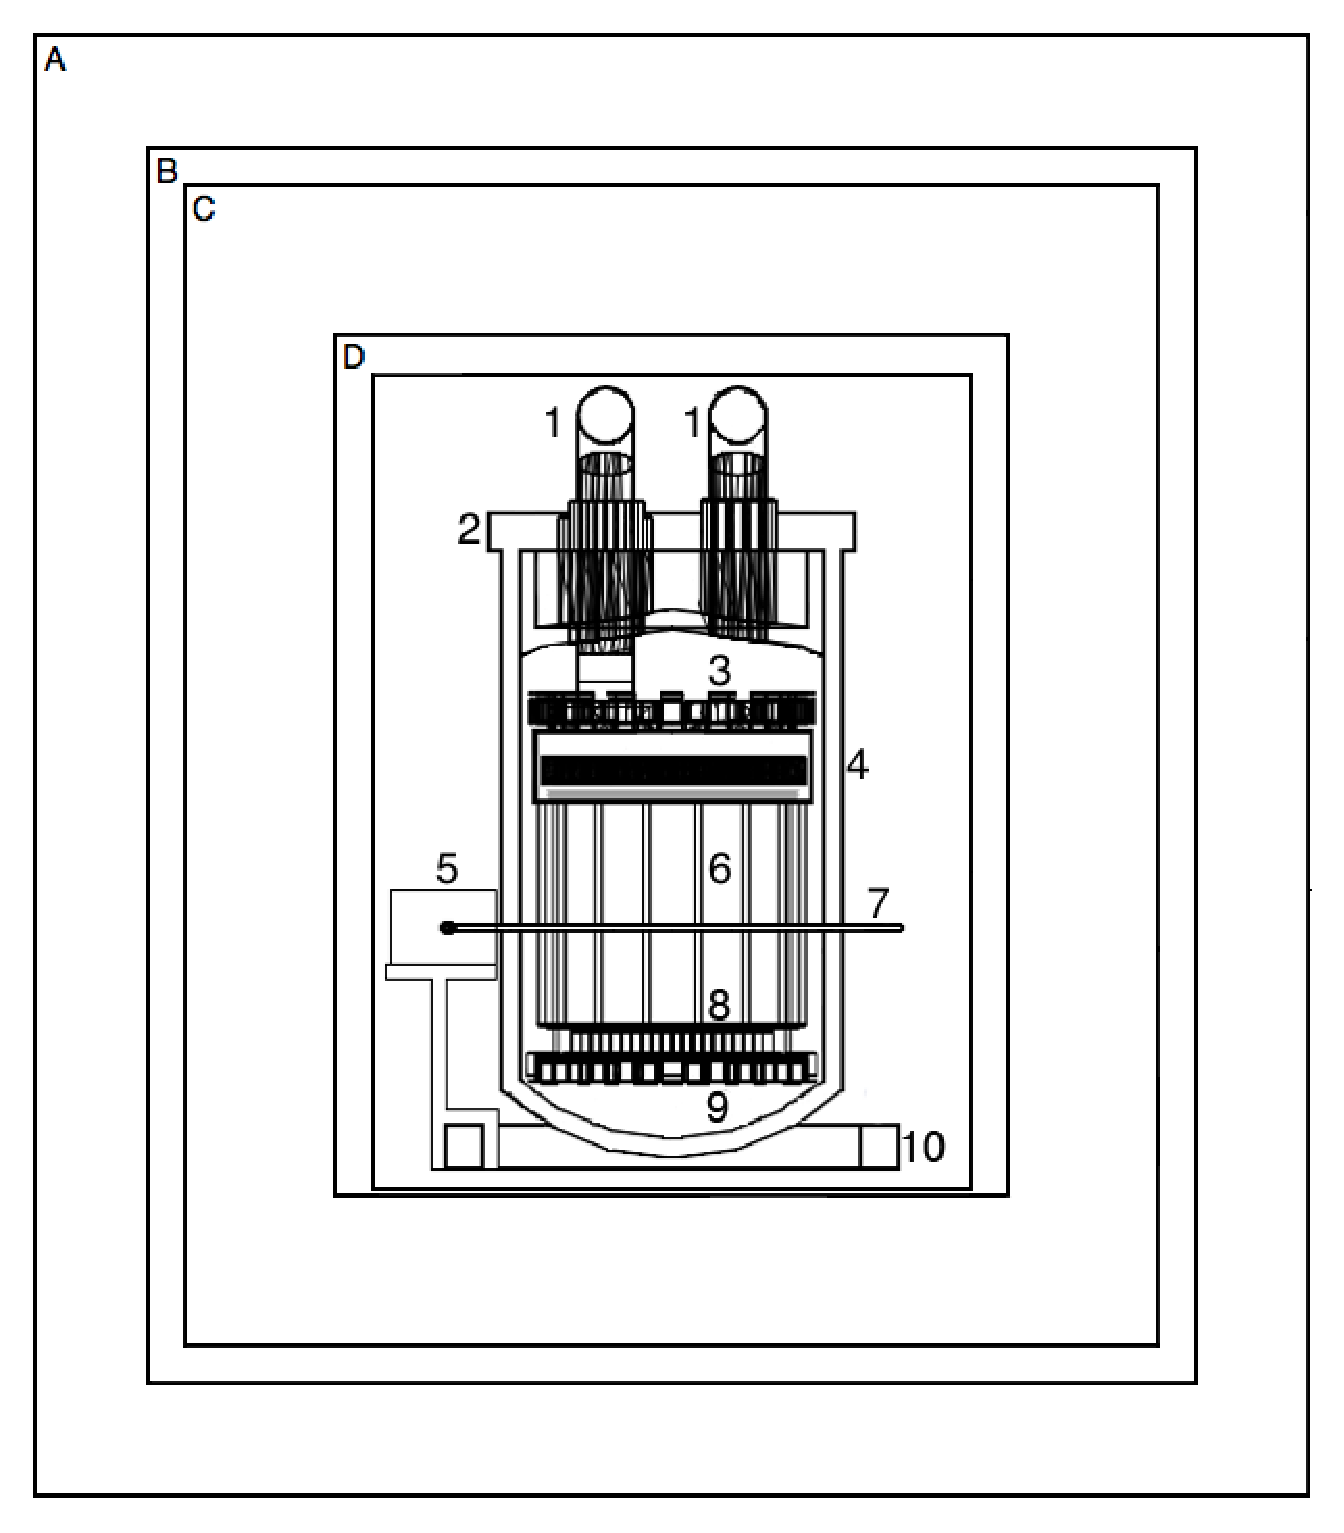
\includegraphics[height=0.5\linewidth]{plots/Geant4model/DetectorModel_shield_withLabels1.eps}
\label{figDetectorModel_1}}
\subfigure[]{
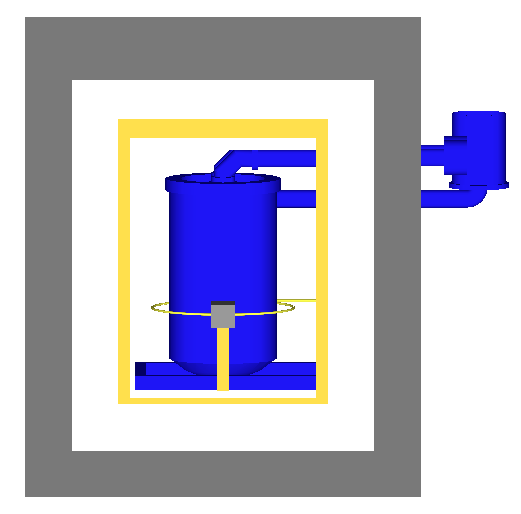
\includegraphics[height=0.51\linewidth]{plots/Geant4model/DetModel_withPTR.png}
\label{figDetectorModel_2}}
\caption[The GEANT4 model of the XENON100 detector and its shield]{The GEANT4 model of the XENON100 detector and its shield: A - outer lead layer, B - inner lead layer with low $^{210}$Pb contamination, C - polyethylene shield, D - copper shield; 1 -  pipes to the PMT feedthroughs and pumping ports, 2 - stainless steel cryostat, 3 - top and upper side veto PMT arrays, 4 - top PMT array in the TPC, in the gas phase inside the `diving bell', 5 - lead brick for calibration with $^{241}$Am-Be neutron source, 6 - TPC wall (PTFE panels), 7 - copper pipe for calibration sources, 8 - bottom PMT array in the TPC, 9 - bottom and lower side veto PMT arrays, 10 - support bars for the cryostat. 
The water shield and an additional polyethylene layer on the bottom are not shown. Figure (a) published in Ref.~\cite{EMBG}.}
\label{figDetectorModel}
\end{figure}

\begin{table}[!ht]
\centering
{\caption{Materials used in the XENON100 experiment, and their properties used in detector  modeling and background predictions}
\label{tabDetectorMaterials}
%\vspace{0.2cm}
\begin{tabular}{>{\footnotesize}l|>{\footnotesize}c|>{\footnotesize}l}
%\begin{tabular}{l | c | l}
\hline
Component 						& Density  			& Chemical composition  \\
								& [g/cm$^{3}$]			& \\
\hline
316Ti stainless steel					& 8.00 		& C 0.08\%, Si 1\%, Mn 2\%, P 0.045\%, S 0.03\%, \\
								&			& Ni 12\%, Cr 17\%, Mo 2.5\%, Ti 4.0\%, Fe 64.945\% \\
PTFE							& 2.20 		& -CF$_{2}$- \\
Copper							& 8.92 		& Cu 100\% \\
$Kovar$ metal						& 8.33 		& Fe 55\%, Ni 29\%, Co 16\%;  \\
Stainless steel						& 7.64 		& Fe 70\%, C 0.1\%, Si 0.5\%, Mn 0.7\%, \\
								& 	 		& Mn 0.7\%, Ni 8.6\%, Cr 18.3\% \\
Synthetic silica						& 2.20 		& SiO$_{2}$ \\
Borosilicate glass					& 2.21 		& SiO$_{2}$ 67.0\%, Al$_{2}$O$_{3}$ 4.3\%, B$_{2}$O$_{3}$ 18.0\%, \\
								&			& Li$_{2}$O 1.0\%, Na$_{2}$O 6.0\%, BaO 2.0\% \\
Aluminum	 (0.1~g/PMT)				& 2.70 		& Al 100\% \\
$Cirlex$							& 1.43 	 	& C$_{22}$H$_{10}$N$_{2}$O$_{5}$ \\
Ceramics							& 1.00		& NaAlSiO$_{2}$ \\
Polyethylene						& 0.92		& -CH$_{2}$- \\
Lead								& 11.34		& Pb 100\% \\
\hline
\end{tabular}
}
\end{table}

The main materials used in the detector model are listed in Table~\ref{tabDetectorMaterials}, together with their density and  chemical composition. Table~\ref{tabDetectorComponents} shows the total weight of detector and shield components, computed from the model and in agreement with the actual detector.



\begin{table}[!h]
\centering
\caption[Components and materials of the XENON100 detector and its shield]{Components and materials of the XENON100 detector and its shield. The total weight of the materials has been calculated with the GEANT4 model.  The cryostat vessels with the top flange and pipes, and the diving bell system are made from the grade 316Ti stainless steel and shown as one unit. The resistive voltage divider network for the TPC drift field is simplified in the model with a thin tube.}
\label{tabDetectorComponents}
%\vspace{0.2cm}
\begin{tabular}{>{\footnotesize}l |>{\footnotesize} r}
%\begin{tabular}{l|r}
\hline
Component 					& Amount of material  \\
\hline
Cryostat and diving bell (316Ti SS) & 73.61 kg 	\\
Support bars (316Ti SS) 			& 49.68 kg 	\\
Detector PTFE 					& 11.86 kg	\\
Detector copper 				& 3.88 kg 		\\
PMTs						& 242 pieces 	\\
PMT bases 					& 242 pieces 	\\
TPC resistor chain 				& 1.5$\times$10$^{-3}$ kg \\
Bottom electrodes (316Ti SS) 		& 0.23 kg 		\\
Top electrodes (316Ti SS) 		& 0.24 kg 		\\
PMT cables					& 1.80 kg 		\\
Copper shield 					& 2.1$\times$10$^{3}$~kg 	\\ 
Polyethylene shield 				& 1.6$\times$10$^{3}$ kg 	\\
Lead shield  (inner layer) 			& 6.6$\times$10$^{3}$ kg 	\\
Lead shield (outer layer) 			& 27.2$\times$10$^{3}$ kg 	\\
\hline
\end{tabular}
\end{table}

In the GEANT4 model, a PMT is simplified with a stainless steel case and a synthetic silica window inside a thin aluminum ring. The ceramic insulator and ZrAl getter are not included due to their low mass (Table~\ref{tabPMTmassModel}). The {\it Cirlex} base for the voltage divider network is approximated as a homogenous unit. 
For background predictions, only the 316Ti SS support rings for the mesh electrodes are considered in the model, given that the meshes are $\sim$100~$\mu$m thick and have a very low mass, leading to a negligible background from their radioactivity. For the photon propagation, the electrode meshes are implemented as 130~$\mu$m thick disks with the appropriate optical transparency.

By default, the entire decay chain simulated with GEANT4 is written into one event, as well as secondary particles, and this leads to pile-up of the energy depositions, and therefore wrong energy spectrum. A custom `G4StackingManagerAction' has been implemented in the XENON100 simulations, which postpones daughter decays to the next event. The total energy deposition for each event is calculated by summing up energy deposited by all primary and secondary particles, which is done separately for the target volume and for the veto. 

For the calculation of the final background rate in the Monte Carlo simulations, multiple scatter events are rejected taking into account the finite position resolution of the detector.  
A multiple scatter event is considered as a single scatter event if the interactions happen less than 3~mm apart in $Z$ (see Section~\ref{secPositionResolution}). This position resolution is given by the width of the S2 signals and the peak separation efficiency of the S2 peak finder algorithm.

%`


\chapter{Light Detection}
\label{chLightDetection}
%\section{Photomultiplier Tubes in the XENON100 experiment}
	\section{Photomultiplier Tubes in the XENON100 experiment}
\label{secPMT}

%\begin{floatingfigure}[l]{0.22\textwidth}
%\begin{figure}[!h]
%\centering
%\subfigure[]{
%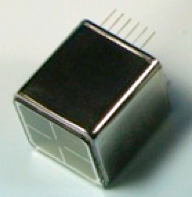
\includegraphics[height=0.2\linewidth]{plots/PMT/R8520.png}
%\label{figPMT_1}}
%\subfigure[]{
%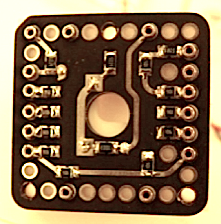
\includegraphics[height=0.2\linewidth]{plots/PMT/PMTbase.png}
%\label{figPMT_2}}
%\caption{R8520-06-AL Hamamatsu PMT (a) and the {\it Cirlex} base with the voltage divider network.}
%\label{figPMT}
%\end{figure}
%\end{floatingfigure}

XENON100 detector utilizes 242 1"-square Hamamatsu PMTs, shown in Fig.~\ref{figPMT_1}. Model R8520-06-AL has been specifically designed to operate in liquid xenon, and to withstand temperature in the range -110 to +50$^{\circ}$C and absolute pressure up to 5~atm. In collaboration with the company, the materials which are used to produce the PMTs have been screened with germanium spectrometers~\cite{ScreeningPaper}, and the design has been optimized to reduce the radioactive contamination.

% joined figure, all 3 pictures together
%\begin{floatingfigure}[l]{0.22\textwidth}
\begin{figure}[!h]
\centering
\subfigure[]{
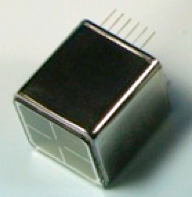
\includegraphics[height=0.20\linewidth]{plots/PMT/R8520.png}
\label{figPMT_1}}
\subfigure[]{
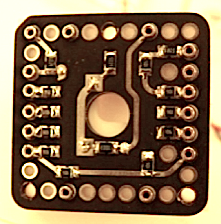
\includegraphics[height=0.20\linewidth]{plots/PMT/PMTbase.png}
\label{figPMT_2}}
\subfigure[]{
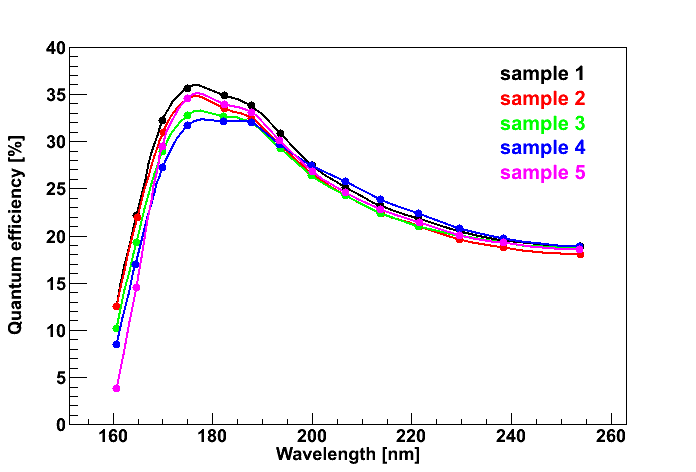
\includegraphics[width=0.475\linewidth]{plots/QE/plotQEvsWL_highQE.png}
\label{figPMT_3}}
\caption[R8520-06-AL Hamamatsu PMT with the voltage divider network on a {\it Cirlex} base, and its quantum efficiency as a function of the wavelength]{R8520-06-AL Hamamatsu PMT (a) with the voltage divider network on a {\it Cirlex} base (b), and quantum efficiency as a function of the wavelength (c)~\cite{PMTmassModel}.}
\label{figPMT}
\end{figure}
%\end{floatingfigure}

%\begin{figure}[!h]
%\centering
%\subfigure[]{
%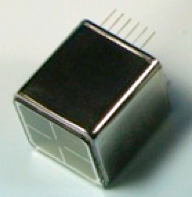
\includegraphics[height=0.2\linewidth]{plots/PMT/R8520.png}
%\label{figPMT_1}}
%\subfigure[]{
%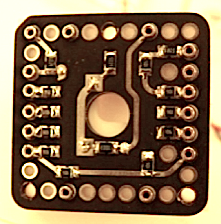
\includegraphics[height=0.2\linewidth]{plots/PMT/PMTbase.png}
%\label{figPMT_2}}
%\caption{R8520-06-Al Hamamatsu PMT (a) and the {\it Cirlex} base with the voltage divider network (b).}
%\label{figPMT}
%\end{figure}

The bialkali photocathode has a minimum effective area of 20.5$\times$20.5 mm, spectral response on the region 160-650~nm and the highest quantum efficiency (QE) for VUV light (see Fig.~\ref{figPMT_3}). The aluminum strips deposited on the window improve the resistivity of the photocathode at cryogenic temperature. The electron multiplier consists of 10 stage metal channel dynode structure. The PMT window is made out of synthetic silica, which has properties of quartz and transmits ultraviolet radiation down to 160~nm. The thermal expansion coefficient of silica is significantly different from that of {\it Kovar} alloy used for the stem pins. The bulb stem is thus made from borosilicate glass, and a graded seal using gradually different thermal expansion coefficient is connected to the synthetic silica bulb. 
The individual components of a R8520-06-AL Hamamatsu PMT are listed together with their total weight in Table~\ref{tabPMTmassModel}~\cite{PMTmassModel}.

Two types of R8520 PMTs are used in the XENON100 detector. The older type (`low QE' PMTs)  that has been also used in XENON10 has an average peak quantum efficiency of 25\%. The newer type of this model (`high QE' PMTs), with an improved photocathode, has a peak quantum efficiency of $\sim$32\% at 175~nm (Fig.~\ref{figPMT_3}).

%\begin{figure}[!h]
%\centering
%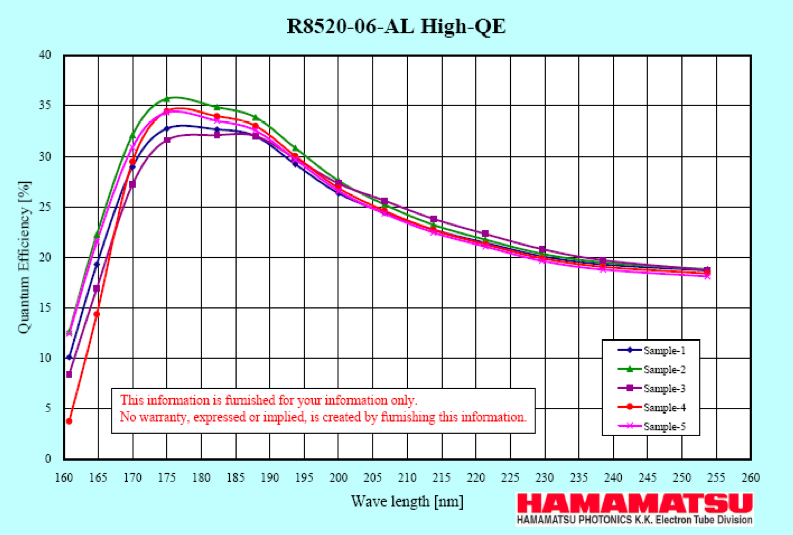
\includegraphics[width=0.475\linewidth]{plots/PMT/Hamamatsu_QEvsWavelength.png}
%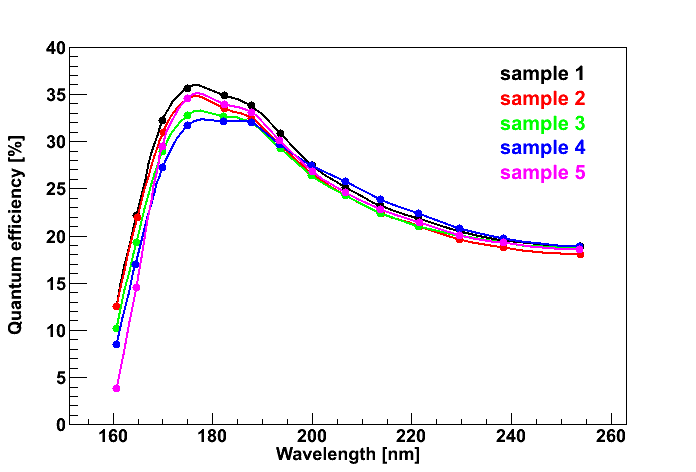
\includegraphics[width=0.475\linewidth]{plots/QE/plotQEvsWL_highQE.png}
%\caption[Quantum efficiency as a function of the wavelength for the 'high QE' Hamamatsu PMTs used in the XENON100 experiment]{Quantum efficiency as a function of the wavelength for the 'high QE' Hamamatsu PMTs used in the XENON100 experiment~\cite[PMTmassModel].}
%\label{figQEhighQE}
%\end{figure}

\begin{table}[!h]
\centering
\caption[Mass model of the R8520-06-AL PMT]{Mass model of the R8520-06-AL PMT \cite{PMTmassModel}.}
\label{tabPMTmassModel}
%\vspace{0.2cm}
\begin{tabular}{>{\footnotesize}l|>{\footnotesize}l|>{\footnotesize}c}
%\begin{tabular}{l|l|c}
\hline
PMT part 					& Material				& Weight [g] \\
\hline
Metal package and stem pins	& {\it Kovar} alloy 		& 13.0	\\
Electrodes				& stainless steel 		& 7.0 \\
Glass for window			& synthetic silica		& 2.0 \\
Glass in stem				& borosilicate glass		& 1.0 \\
Aluminum ring				& Al 					& 0.1	 \\
Insulator					& ceramic				& 0.04 \\
Getter					& ZrAl				& 0.02 \\
\hline
\end{tabular}
\end{table}

A PMT is supplied with high voltage via {\it Kapton} insulated wires. The voltage divider network, which is used to distribute the high voltage supplied to a PMT and provide a proper voltage gradient to each dynode, is shown in Fig.~\ref{figPMT_2}. It consists of 13 surface mount resistors and a capacitor, soldered on a substrate (base) made out of {\it Cirlex}~\cite{cirlex}. The cables used for the PMT signal are RG174 model, consisting of the copper conductor in PTFE isolation with a tinned copper shield~\cite{RG174cable}. The estimated total length of the cables in the detector is 530~m, with corresponds to a weight of 1.8~kg. 

The top array on the target volume consists of 98 PMTs, mounted in a concentric pattern inside the diving bell. The PMTs are installed in the PTFE disk-like structure (Fig.~\ref{figTopArray_1}) and are held on the top with oxygen-free high thermal conductivity (OFHC) copper rings (Fig.~\ref{figTopArray_2}).


\begin{figure}[!h]
\centering
\subfigure[]{
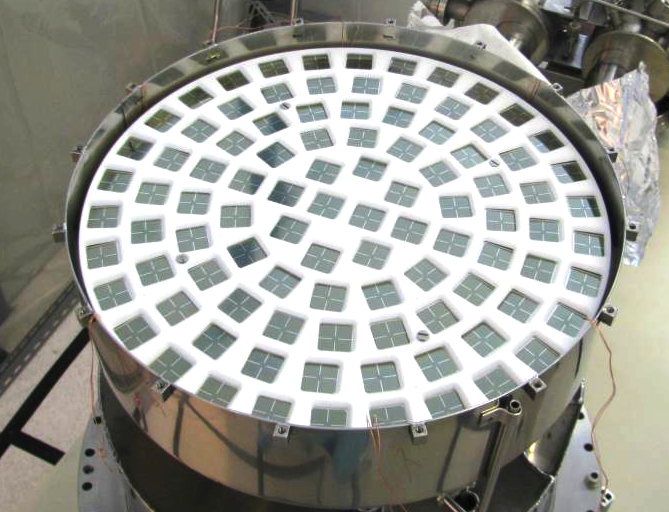
\includegraphics[height=0.3\linewidth]{plots/PMT/TopPMTarray_front.png}
\label{figTopArray_1}}
\subfigure[]{
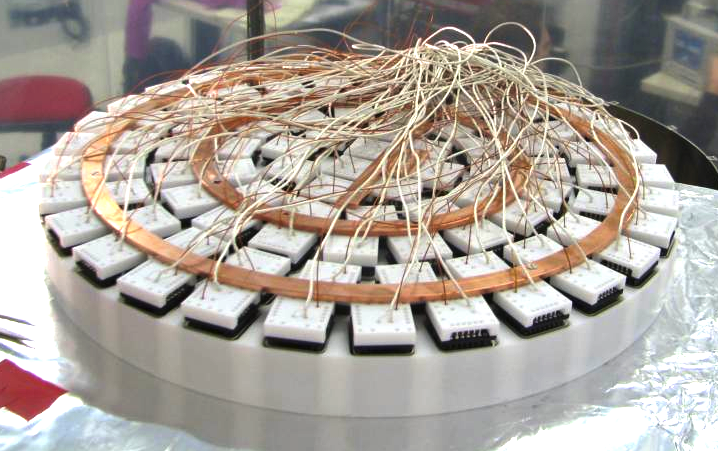
\includegraphics[height=0.3\linewidth]{plots/PMT/TopPMTarray_rear.png}
\label{figTopArray_2}}
\caption[Front and rear views of the top PMT array]{Front (a) and rear (b) views of the top PMT array, installed inside the diving bell in a PTFE structure with a copper support.}
\label{figTopArray}
\end{figure}

\begin{figure}[!h]
\centering
\subfigure[]{
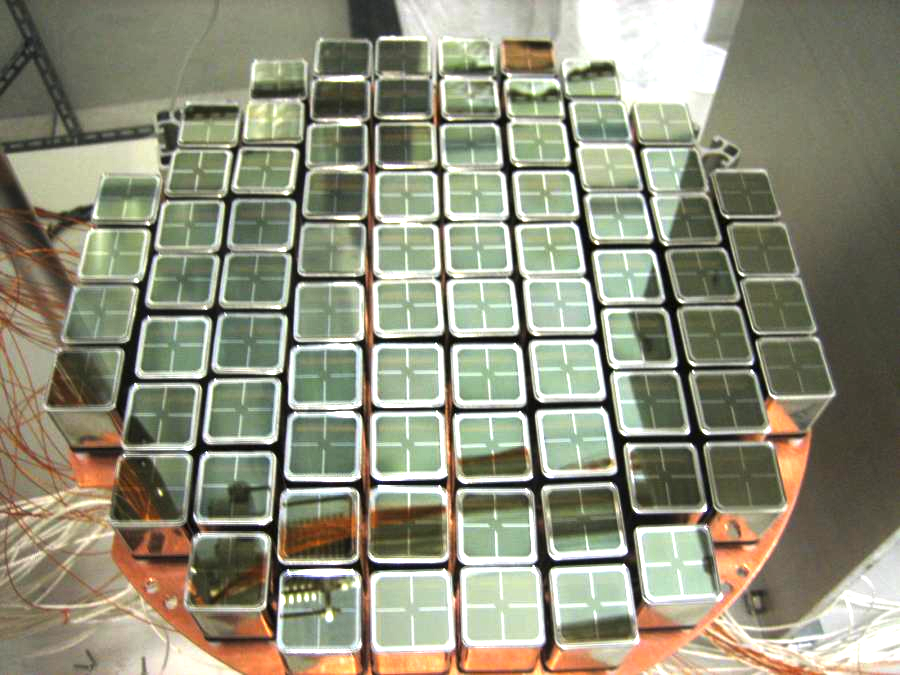
\includegraphics[height=0.3\linewidth]{plots/PMT/BottomPMTarray_front.png}
\label{figBottomArray_1}}
\subfigure[]{
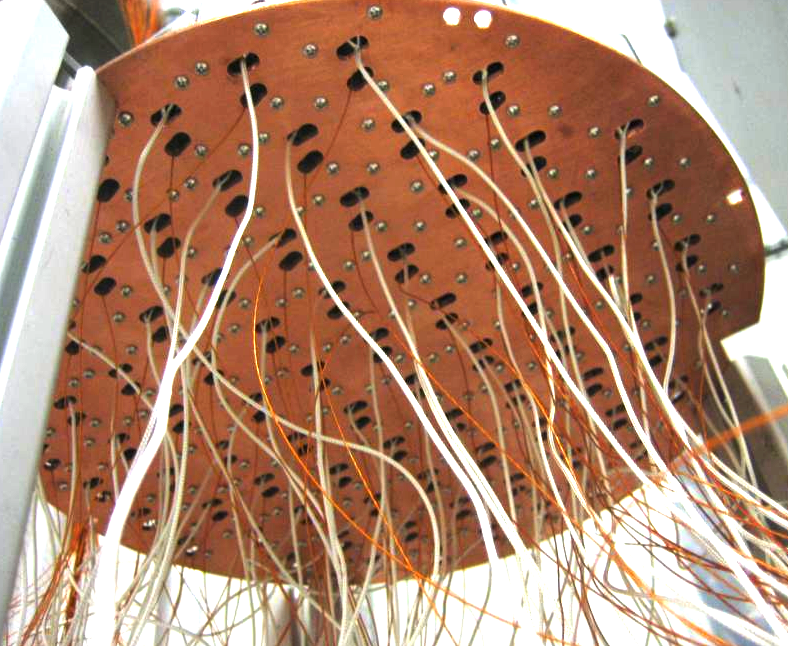
\includegraphics[height=0.3\linewidth]{plots/PMT/BottomPMTarray_rear.png}
\label{figBottomArray_2}}
\caption[Bottom PMT array in the target volume]{Bottom PMT array in the target volume (a), mounted on a copper plate (b).}
\label{figBottomArray}
\end{figure}

The bottom PMT array consists of 80 PMTs, mounted in a rectangular pattern in order to maximize the photocathode coverage (Fig.~\ref{figBottomArray_1}). They are mounted on a OFHC copper plate (Fig.~\ref{figBottomArray_2}).

The veto volume is equipped with 64 PMTs mounted on the copper angles and alternating the direction (Fig.~\ref{figVetoArrays}). 32 of them observe the sides from the top and bottom, and 32 PMTs view the veto volume above and below the TPC.

\begin{figure}[!h]
\centering
\subfigure[]{
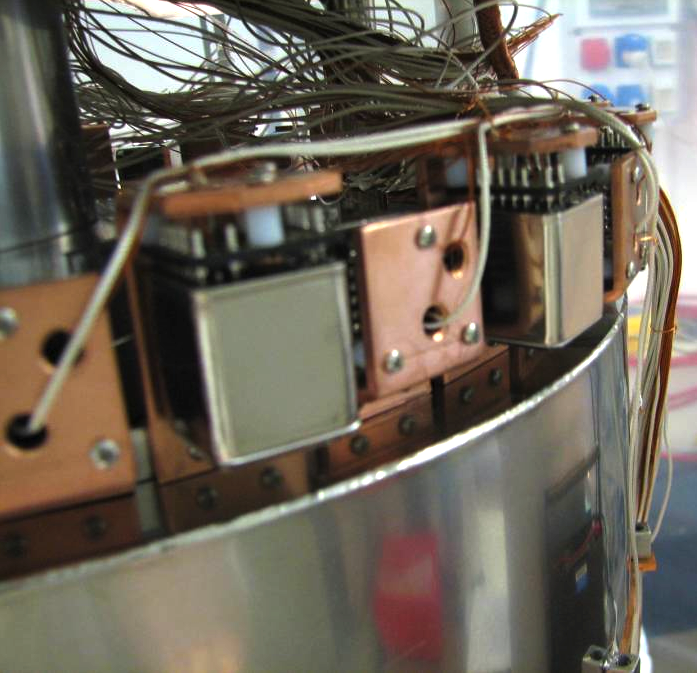
\includegraphics[height=0.3\linewidth]{plots/PMT/VetoTopPMTarray.png}
\label{figVetoArrays_1}}
\subfigure[]{
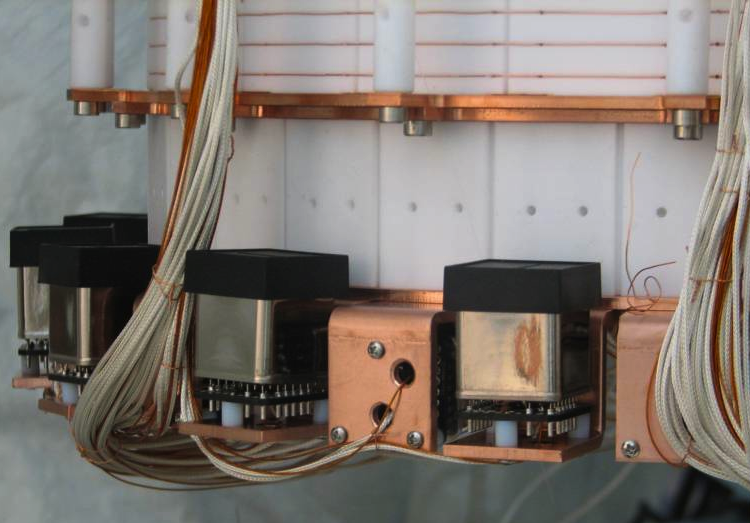
\includegraphics[height=0.3\linewidth]{plots/PMT/VetoBottomPMTarray.png}
\label{figVetoArrays_2}}
\caption[PMT arrays in the veto volume]{PMT arrays in the veto volume: (a) - top and upper side; (b) - bottom and lower side.}
\label{figVetoArrays}
\end{figure}

The arrangement of the PMTs within the target volume and veto arrays is shown in Fig.~\ref{figPMTarrangement}. 
At the beginning of the commissioning run in Fall~2009, 8 PMTs stopped working, mostly due to a connection problem or a shortcut inside the cryostat. For some of the PMTs, an increase of the dark current rate has been observed shortly before the failure, which might indicate a progressive deterioration of the vacuum sealing.

\begin{figure}[!h]
\centering
\subfigure[top]{
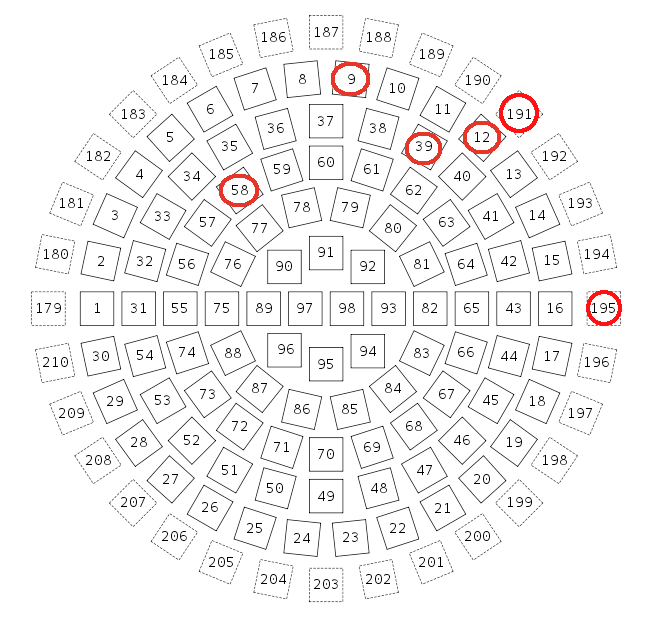
\includegraphics[height=0.425\linewidth]{plots/PMT/topPMTs.png}
\label{figPMTarrangement_1}}
\subfigure[bottom]{
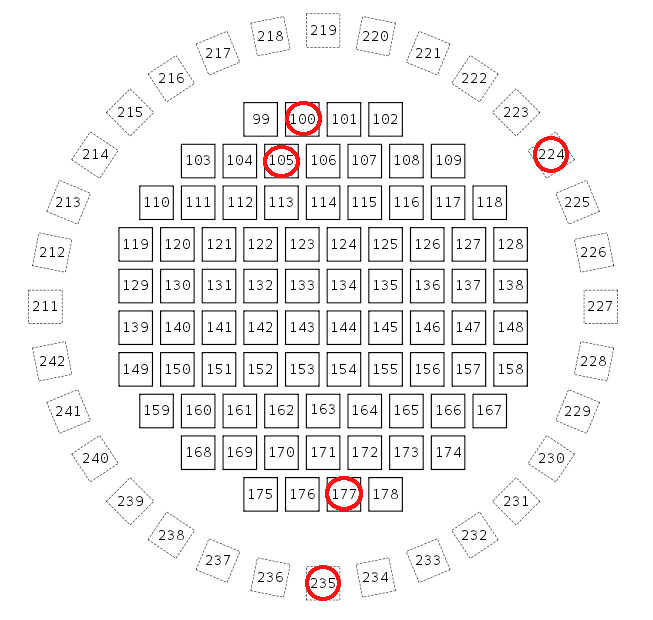
\includegraphics[height=0.425\linewidth]{plots/PMT/bottomPMTs.png}
\label{figPMTarrangement_2}}
\caption[The arrangement of the PMTs within the detector arrays]{The arrangement of the PMTs within the detector arrays. PMTs 1-98 - top array in the target, 99-178 - bottom array in the target, 179-210 - top and upper side arrays in the veto, 211-242 - bottom and lower side arrays in the veto. The red circles show the channels that are not functioning.}
\label{figPMTarrangement}
\end{figure}



%\section{PMT Characterization in Room Temperature}
	\section{PMT Characterization at Room Temperature}
\label{PMTtest}

The PMTs were tested in order to determine their functionality, which was done by the measurement of several parameters. The PMT gain is determined as the mean number of electrons produced by a phototube in response to one photoelectron (PE). The PMT signal (integrated charge spectrum) has been fitted by a sum of an exponential and  a gaussian functions, or, in case of presence of a double photoelectron peak, by a sum of an exponential and two gaussian functions (see Fig.~\ref{figPMTtestSER}). Single PE resolution of a phototube has been calculated as the width ($\sigma$) of the single PE peak, divided by its mean. The `peak-to-valley' ratio is calculated as the ratio of the height of the single PE peak and the valley after the pedestal, and thus quantifies the separation of the noise and signal. These measured quantities characterize the ability to reduce the drift effects of the PMT sensitivity and supply voltage fluctuations, when the tube is operated over extended time periods. 

The facility for PMT testing and characterization has been assembled according to the scheme shown in Fig.~\ref{figPMTtestScheme}. The light tight box with 6 channels provides a possibility to test 5 PMTs simultaneously. During the whole period of the test one PMT has been constantly located in the same spot (channel 5 in the light tight box) and tested in every measurement cycle for calibration purpose, in order to determine possible systematic errors of the measurements. 

\begin{figure}[!ht]
\centering
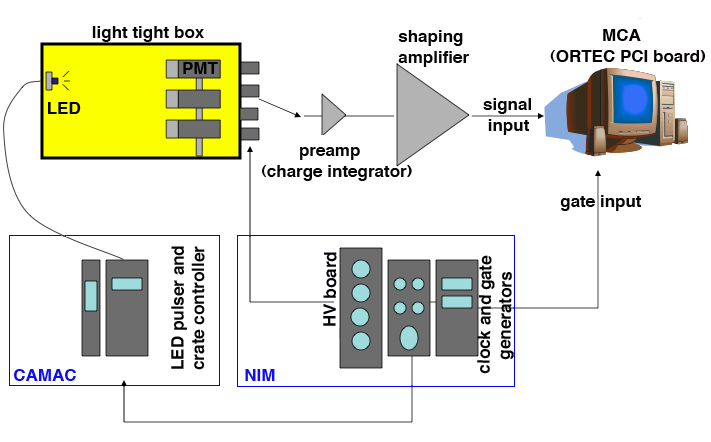
\includegraphics[width=0.8\linewidth]{plots/PMTtest/PMTtestSetupFlip_withLabels.png}
\caption[Schematic diagram of the PMT test facility]{Schematic diagram of the PMT test facility.}
\label{figPMTtestScheme}
\end{figure}

In total, 218 PMTs have been tested. Among them, there are 126 low QE phototubes purchased for the XENON100 detector, 34 low QE PMTs that have been used in the XENON10 experiment, and planned to be installed in XENON100 or kept as spare for possible replacements, and 58 high QE PMTs, with an improved photocathode and QE increased by almost 50\% in average.

The examples of the single PE response measured at room temperature are shown in Fig.~\ref{figPMTtestSER_1} and Fig.~\ref{figPMTtestSER_2}, for one of the PMTs with a good characteristics and considered to be installed in the XENON100 detector, and for one of the PMTs with bad separation between noise and signal and not used in the experiment. Out of 126 low QE PMTs, 4 PMTs did not show a signal, and have been classified as not working and returned to the factory.

\begin{figure}[!t]
\centering
\subfigure[]{
%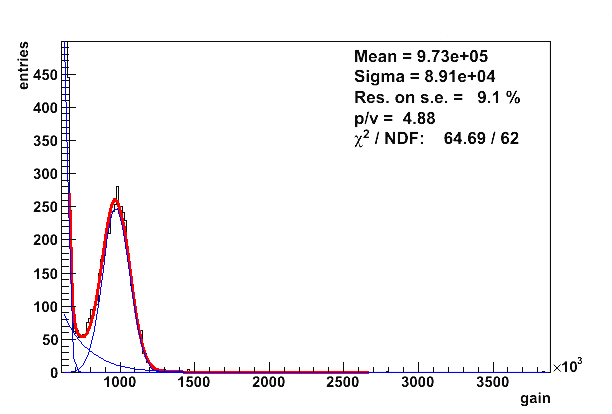
\includegraphics[width=0.475\linewidth]{plots/PMTtest/PMTtest_GoodPMT.png}
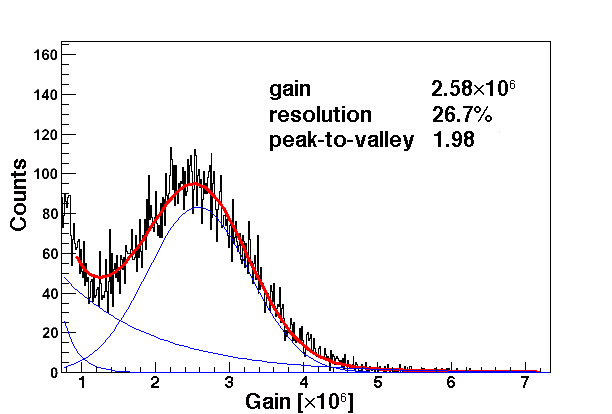
\includegraphics[width=0.475\linewidth]{plots/PMTtest/GoodPMTspectrum1.png}
\label{figPMTtestSER_1}}
\subfigure[]{
%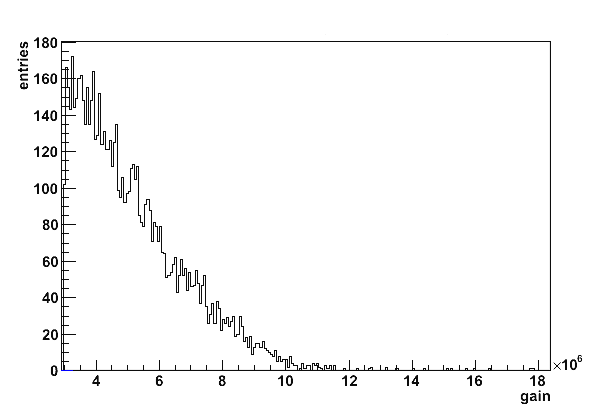
\includegraphics[width=0.475\linewidth]{plots/PMTtest/PMTtest_BadPMT.png}
\includegraphics[width=0.475\linewidth]{plots/PMTtest/BadPMTspectrum1.png}
\label{figPMTtestSER_2}}
\caption[Single photoelectron response of the R8520 Hamamatsu phototubes, measured in the room temperature]{Single photoelectron response of the R8520 Hamamatsu phototubes, measured in the room temperature: (a) - typical single PE spectrum of a PMT chosen to be used in XENON100; (b) - response of the PMT not used in the experiment due to low peak-to-valley ratio, and hence bad separation between noise and signal.}
%PMT with a bad single PE response, peak-to-valley ratio around 1, not used in the experiment.}
\label{figPMTtestSER}
\end{figure}

The gain has been measured with a different high voltage supplied to each PMT (Fig.~\ref{figGainVShv_1}). The current amplification increases proportional to the exponential power of the supply voltage:

\begin{equation}
\mathrm{gain} = A \cdot V^{kn},
\end{equation} 
where $A$ is a constant, $V$ - supply voltage, $n$ - number of dynodes, and $k$ - constant determined by the structure and material of the electrodes. 
The single PE resolution becomes improves with an increase of PMT gain, as shown in Fig.~\ref{figGainVShv_2}.

\begin{figure}[!t]
\centering
\subfigure[]{
\includegraphics[width=0.475\linewidth]{plots/PMTtest/gainVShv.png}
\label{figGainVShv_1}}
\subfigure[]{
%\includegraphics[width=0.475\linewidth]{plots/PMTtest/QualityFactor.png}
\includegraphics[width=0.475\linewidth]{plots/PMTtest/resVSgain.png}
\label{figGainVShv_2}}
\caption[Measured PMT gain as a function of the supply voltage and the correlation between single photoelectron resolution and  gain]{Measured PMT gain as a function of the supply voltage (a), and correlation between the single photoelectron resolution and the gain (b).}

% and the quality factor, defined as the ratio of the peak-to-valley ratio and the single photoelectron resolution, which correspond to PMT gain of $\sim$2$\times$10$^{6}$.}
\label{figGainVShv}
\end{figure}


No major changes have been observed between the low QE and high QE batches of PMTs in the mean values of peak-to-valley ratio and single PE resolution. However, as shown in Fig.~\ref{figPMTtestCorrelation_2}, the average gain of low QE PMTs is almost twice higher than that of the high QE ones, measured at the same supply voltage. This effect is also present within the PMTs of the same batch: there is a  correlation between the measured gain at fixed voltage and QE, provided by the manufacturer for each PMT. It is indicated with a thick blue line in Fig.~\ref{figPMTtestCorrelation_2}. This anti-correlation between QE and gain parameters could not be explained, and might be a product of the systematics of the spectral response measurements performed by the manufacturer.

%\begin{figure}[!h]
%\centering
%\subfigure[]{
%\includegraphics[width=0.475\linewidth]{plots/PMTtest/lowQE_highQE_xe10_GAIN.png}
%\label{figPMTtestResults_1}}
%\subfigure[]{
%\includegraphics[width=0.475\linewidth]{plots/PMTtest/lowQE_highQE_xe10_RES.png}
%\label{figPMTtestResults_2}}
%\subfigure[]{
%\includegraphics[width=0.3\linewidth]{plots/PMTtest/lowQE_highQE_xe10_PV.png}
%\label{figPMTtestResults_3}}
%\caption[Results of the PMT tests in room temperature for different PMT batches]{Results of the PMT tests in room temperature for different PMT batches: (a) - gain at fixed supply voltage of 900~V, (b) - resolution on single PE.
%, (c) - peak-to-valley ratio.
%}
%\label{figPMTtestResults}
%\end{figure}


\begin{figure}[!h]
\centering
\subfigure[]{
%\includegraphics[width=0.475\linewidth]{plots/PMTtest/122lowQE_SKBvsGAIN_zoom.png}
%\includegraphics[width=0.475\linewidth]{plots/PMTtest/resVSgain.png}
\includegraphics[width=0.475\linewidth]{plots/PMTtest/gainVSqe_LowHigh_withLines.png}
\label{figPMTtestCorrelation_1}}
\subfigure[]{
%\includegraphics[width=0.475\linewidth]{plots/PMTtest/122lowQE_resVSgain.png}
%\includegraphics[width=0.475\linewidth]{plots/PMTtest/gainVSqe.png}
\includegraphics[width=0.475\linewidth]{plots/PMTtest/QualityFactor_LowHigh.png}
\label{figPMTtestCorrelation_2}}
\caption[Correlation between the PMT gain measured at fixed voltage and quantum efficiency provided by the manufacturer, and the PMT test quality factor]{(a) - correlation between the PMT gain measured at fixed voltage (800~V) and quantum efficiency (QE) provided by the manufacturer. The vertical and horizontal dashed lines show the average gain and QE, respectively. The thick blue line is a fit to the low QE PMTs data points. (b) - the quality factor, defined as the ratio of the peak-to-valley ratio and the single photoelectron resolution, which correspond to PMT gain of $\sim$2$\times$10$^{6}$.}
\label{figPMTtestCorrelation}
\end{figure}

In addition to the measurement of PMT characteristics, all high QE phototubes have been tested to withstand the thermal shocks from room to cryogenic temperature using dry ice (solid carbon dioxide, temperature $-$78.5$^{\circ}$C). This has been necessary, as these PMTs have been produced specifically for XENON100 using a new type of vacuum sealing, and potential problems have been reported by the manufacturer. Out of the 58 PMTs that have undergone the cooling test, 10 PMTs showed problems (discharge while raising the supply voltage or absence of signal), and have been returned to the factory for a replacement.

For all PMTs classified as working after the tests, a `quality factor' has been defined as the ratio of the measured peak-to-valley ratio and resolution on single PE. The distribution of this parameter is shown in Fig.~\ref{figPMTtestCorrelation_2} and centered around 0.3 for both low QE and high QE PMT batches. In addition to QE, this quality factor has been used to compare the PMTs and distribute them within the different arrays in the detector. All high QE PMTs have been placed on the bottom array in the target volume to ensure that the detected light yield (S1) is as high as possible. The phototubes with the highest QE have been placed in the center of the array. The `low QE' PMTs have been placed on the top array in the target volume in the veto.




%\section{PMT Gain Calibration}
%\subsection{Hardware Setup}
%\subsection{Analysis and Monitoring Software}
	\section{Light Calibration During Detector Operation}
\label{secGainCalibration}


The analysis of the experimental data of XENON100 requires the detailed characterization of 242 individual channels. PMT calibration is performed regularly for this purpose, by stimulating single  photoelectron emission from the photocathode with a light-emitting diode (LED) light. The main goal of the light calibration is to measure the absolute gain of every channel, and monitor the response over time. Several additional parameters are also determined, such as the single photoelectron resolution, peak-to-valley, and signal-to-noise ratios.

A dedicated system has been developed for the light calibration of the PMTs in the XENON100 detector, including the hardware setup with an external LED source, and the analysis and monitoring software: ROOT-based C++ programs for the data processing and analysis of the single photoelectron response, a dynamic database, and a web-based visualization tool. 

%\subsection{Hardware Setup}
%\label{secGainCalibrationHardware}

%\begin{floatingfigure}[r]{0.6\textwidth}
\begin{figure}[!t]
\centering
\includegraphics[width=1.0\linewidth]{plots/PMTcalibration/CalibrationSchemeFull.png}
\caption[Schematic of the setup for PMT calibration]{Schematic of the setup for PMT calibration, which consists of hardware setup with an external LED with the optical fiber light guides, and the analysis and monitoring software.}
\label{figCalibrationSetup}
\end{figure}
%\end{floatingfigure}

The hardware system for the PMT calibration with LEDs has been set up as shown in Fig.~\ref{figCalibrationSetup}. An external clock is connected to the DAQ trigger input with a NIM signal, and the TTL output is sent to the pulse generator (LED driver). The LED driver provides two output channels connected to a light-tight box with two InGaN LEDs, which emit blue light  with an average wavelength of 470~nm. The light from the LEDs is transferred by two standard coated optical fibers (1~mm core) to optical feedthroughs on the detector flange. At the vacuum side of the feedthroughs, two uncoated quartz fibers are connected (800~$\mu$m core), which direct the light into the detector volume. Quartz is chosen for its high melting point, which allows  the pipes to be baked at higher temperatures (up to 200$^{\circ}$C). In order to diffuse the light and to achieve a uniform illumination of all PMTs, the quartz fibers are connected inside the cryostat to two bundles of polymethylmethacrylate (PMMA-PFA) fibers with 180~$\mu$m core. PMMA-PFA optical fiber is more flexible than quartz, thus well suited for small bending radii inside the cryostat. The coating has been removed from the fibers, in order to minimize the amount of materials placed in liquid xenon. Temperature resistance is not crucial for these inner fibers, because the baking temperature is limited by the allowed range for the PMTs (50$^{\circ}$C). A `1-to-4' optical fiber bundle is used to illuminate top and bottom PMT arrays in the target volume, and a `1-to-6' bundle guides the light into the veto volume. Two branches of the veto bundle are used for PMTs on the top and bottom of the veto volume, and four remaining ones are used to illuminate the side veto PMTs.

%\begin{figure}[!h]
%\centering
%\subfigure[]{
%\includegraphics[width=0.475\linewidth]{plots/PMTcalibration/PMT131_wf.png}
%\label{figPMTwf_1}}
%\subfigure[]{
%\includegraphics[width=0.475\linewidth]{plots/PMTcalibration/dc1_vs_time_PMT146.png}
%\label{figPMTwf_2}}
%\caption{(a) - a waveform of the PMT signal recorded during the calibration run, after baseline subtraction. (b) - a long-term dark current rate evolution for one of the XENON100 PMTs. }
%\label{figPMTwf}
%\end{figure}

The total amount of light produced by an LED depends on the amplitude of the voltage pulse and on its time width. In order to achieve single PE level for PMT illumination, the amplitude of the pulse has been set to the minimum required to turn on the LED. If the time delay between the light signals is shorter than the time necessary to restore the initial condition on each dynode, this might produce drift effects on the PMT gain. Thus, a relatively low pulse rate of 100~Hz is used, which still allows the acquisition of reasonable statistics in a short time: 100'000 events take about 20~min, with an average of $\sim$1'000 signal pulses per PMT. 

The width of the pulse is 4~$\mu$s, and the total digitization window is 5~$\mu$s. The data is acquired without zero length encoding. The DAQ has been set such that 1~$\mu$s (100 samples) is acquired before the trigger, in order to compute the baseline for each event by averaging the ADC counts. 
The signal rate in the pre-trigger part of the digitized waveform is additionally used to monitor `dark count' rate of the PMTs. Even though some signals are always present when the scintillator medium is present in the detector, this provides a possibility to monitor the PMT functionality. 
%The typical waveform of the PMT signal after baseline subtraction is shown in Fig.~\ref{figPMTwf_1}. 
% An example of the long-term dark current rate evolution for one of the XENON100 PMTs is shown in Fig.~\ref{figPMTwf_2}. 

Ideally, all PMTs should be uniformly illuminated, so that each phototube detects light on the level of single PE. Since the optical fibers for illumination of the inner PMTs are installed in the liquid phase, the light from an LED is reflected on the liquid surface, and the amount of light on the top array is significantly lower than on the bottom PMT array (Fig.~\ref{figLightLevel_1}). In addition, its maximum is not synchronized in time for both PMT arrays. The difference in light level is also present for the PMTs within the same array, due to geometrical effects and differences in the QE of the phototubes.
%The typical waveform of the PMT signal after baseline subtraction is shown in Fig.~\ref{figLightLevel_2}. 

%\begin{floatingfigure}[r]{0.6\textwidth}
\begin{figure}[!h]
\centering
\subfigure[]{
\includegraphics[width=0.475\linewidth]{plots/PMTcalibration/ADCvsSMPmod.png}
\label{figLightLevel_1}}
\subfigure[]{
\includegraphics[width=0.47\linewidth]{plots/PMTcalibration/PMTcalibrationWindow_withLEDpulse.png}
\label{figLightLevel_2}}
\caption[Light level on the top and bottom PMT arrays in the target volume, and a typical waveform of the PMT signal]{(a) - Light level on the top and bottom PMT arrays in the target volume as a function of the data acquisition time within one event; 1~sample~=~10~ns. (b) - a typical waveform of the PMT signal, with an indicated software cut for the pulse search window.}
\label{figLightLevel}
\end{figure}
%\end{floatingfigure}

In order to equalize the amount of light detected by each phototube, a software cut on the calibration window size has been developed, which allows reduction of multiple PE emission within one event (Fig.~\ref{figLightLevel_2}). The number of samples in the calibration window shown in Fig.~\ref{figLightLevel_2} is adjusted for each PMT in such a way that the ratio of the number of triggers with no detected signal and the total number of triggers does not exceed 95\%. Brightly illuminated PMTs have a short search window, and dimly illuminated a longer one, up to full length of the LED pulse (4~$\mu$s).

%\begin{figure}[!h]
%\centering
%\includegraphics[width=0.5\linewidth]{plots/PMTcalibration/BlueLEDSpectrum.png}
%\caption{Spectral response of InGaN ('blue') LED.}
%\label{figLEDspectrum}
%\end{figure}

%\subsection{Analysis and Monitoring Software}
%\label{secGainCalibrationSoftware}

The first stage of the data analysis includes processing of the raw data, which produces a ROOT file storing the content in ADC counts of 10 bins across the maximum with subtracted baseline.

At the second stage, the pulse area is calculated from the integrated pulse height, and the PMT response is analyzed. An example of the spectrum induced by the LED light is shown as integrated ADC counts in Fig.~\ref{figPMTresponse_1}. The response of the PMT is described by a sum of two functions, describing the noise peak (pedestal), and single PE peak. The noise peak is usually fitted by a Gaussian function, and the single PE peak is described by a continuous distribution in the form~\cite{SPEfit1, SPEfit2}:
\begin{equation}
\label{ContinuousDistribution}
y = \frac{\mu^x \cdot e^{-\mu}}{\Gamma[x+1]},
\end{equation}
where $y$ is the number of counts/channels in the spectrum, $x$ is the ADC value, $\mu$ is the mean of the Poisson distribution, and $\Gamma$ is the gamma function, given by:
\begin{equation}
\label{GammaFunction}
\Gamma[x] = \int t^{x-1}\ e^{-t}\ dt.
\end{equation}

The integrated ADC counts are converted to PMT gain as following:

\begin{equation}
\mathrm{gain} = \frac{\mu \cdot r}{Z \cdot A \cdot f \cdot e},
\end{equation}
where $\mu$ - mean of the single PE peak in ADC counts;
$r$~=~2.25/2$^{14}$~[V/bit] - ADC resolution;
$Z$~=~50~[Ohm] - input impedance; 
$A$~=~10 - amplification factor for PMT signal; 
$f$~=~10$^{8}$~[s$^{-1}$] - sampling frequency; 
$e$~=~1.60218$\cdot$10$^{-19}$~C - electron charge.

The typical dark current spectrum of a XENON100 PMT during detector operation is shown in Fig.~\ref{figPMTresponse_2}. The dark current is calculated in different ranges: for the pulses more than 6$\sigma$ away from noise peak, based on a Gaussian fit of the latter, for the pulses with an amplitude 200-700 ADC counts, 300-700 ADC counts, and $>$700 ADC counts.

\begin{figure}[!h]
\centering
\subfigure[]{
\includegraphics[height=0.4\linewidth]{plots/PMTcalibration/PMTsinglePE.png}
\label{figPMTresponse_1}}
\subfigure[]{
\includegraphics[height=0.4\linewidth]{plots/PMTcalibration/PMTdc_clean.png}
\label{figPMTresponse_2}}
\caption[Response of a XENON100 PMT to an LED light and a typical dark current spectrum]{Response of a XENON100 PMT to an LED light (a) and a typical dark current spectrum (b).}
\label{figPMTresponse}
\end{figure}

For most of the PMTs, a Gaussian function is a good approximation of the noise distribution. However, on some of the channels electronic noise with different amplitudes and frequencies has been observed. In this case, the random position and width of the PMT pulses at the pedestal peak does not allow use of a general function to fit the noise part of the spectrum. The origin of the electronic noise is a pick-up on high voltage line, thus the noise is correlated on the channels which are connected through to the same HV board or filter box. The light signal on all channels is on the contrary not correlated, which provides a method to discriminate electronic noise. Such noise removal technique is used for the PMTs 1 and 2, installed in the top PMT array (see Fig.~\ref{figNoiseDiscrimination_1}). The spectrum of the PMT1 is shown with a blue histogram in Fig.~\ref{figNoiseDiscrimination_2}. The amplitude and frequency of the electronic noise on this channel are so high that it significantly overlaps with the signal distribution, and the PMT gain cannot be determined. Using the cut on the correlation of the pulse height between channels 1 and 2, it is possible to completely remove the noise population and get the clean single PE distribution. However, some part of low amplitude signal pulses are removed, and the measured gain is biased to slightly higher values.

\begin{figure}[!h]
\centering
\subfigure[]{
\includegraphics[height=0.4\linewidth]{plots/PMTcalibration/CorrelatedNoise_PMT1-2.png}
\label{figNoiseDiscrimination_1}}
\subfigure[]{
\includegraphics[height=0.4\linewidth]{plots/PMTcalibration/PMT1_withNoiseCut.png}
\label{figNoiseDiscrimination_2}}
\caption[Discrimination of the correlated electronic noise]{Discrimination of the correlated electronic noise: (a) - discrimination parameter; (b) - spectrum of PMT1 without (blue) and with (black) noise cut, together with the single PE fit (red).}
\label{figNoiseDiscrimination}
\end{figure}

The gain calibration is performed weekly, and fits of all the 242 PMTs are visually inspected to ensure the fit quality. For this purpose, a web-based tool with an interactive PMT map has been developed. The output of the analysis is written into a dynamic MySQL database, which allows the data processing software to automatically take into account changes in the PMT characteristics. 

The gains of all PMTs in the XENON100 detector have been equalized to approximately 2$\times$10$^{6}$ (Fig.~\ref{figGainDistribution_1}), which corresponds to an average area of a single PE peak of $\sim$120 ADC counts. An example of the long-term stability of the PMT gain is shown in Fig.~\ref{figGainDistribution_2}. The average gain of the XENON100 PMTs is 1.96$\times$10$^{6}$ with the differences between the channels on the order of 10\%, and is stable over time within $\pm$2\% ($\sigma/\mu$), which is comparable with the statistical error of the gain determination (1.6\%). The distribution of the peak-to-valley ratio is centered at 52\%, and the resolution on the single PE is on average 52\%.

\begin{figure}[!h]
\centering
\subfigure[]{
%\includegraphics[width=0.475\linewidth]{plots/PMTcalibration/gr_gain.png}
\includegraphics[width=0.475\linewidth]{plots/PMTcalibration/h_gain1.png}
\label{figGainDistribution_1}}
\subfigure[]{
\includegraphics[width=0.475\linewidth]{plots/PMTcalibration/gain_vs_time.png}
\label{figGainDistribution_2}}
\caption[The equalized gains of the XENON100 PMTs and an example of the long-term stability]{The equalized gains of the XENON100 PMTs (a) and an example of the long-term stability for one of them (b). The horizontal blue lines indicate the RMS  spread over an 8 month period. It is comparable with the statistical errors of the measurements.}
\label{figGainDistribution}
\end{figure}


% , because it is  A methods have been developed in order to discriminate the electronic noise on such PMTs.

% One of them is based on pulse shape analysis of the digitized waveform, using as a discrimination parameter the ratio between the height of the peak and the summed counts in the integration window (Fig.~\ref{figNoiseDiscrimination}). However, such a cut removes together with noise the signal pulses with lower amplitude, and the gain calculated with this method is biased towards higher values. The second method is used for the channels on which the noise is 




%`


	\section{Detection Efficiency of the XENON100 PMTs}
\label{secQE}

The spectral response of a PMT can be characterized by the radiant sensitivity or with a QE of the photocathode. 
Radiant sensitivity is the photoelectric current from the photocathode normalized to the incident flux at a given wavelength. QE is the ratio of photoelectrons emitted from the photocathode and the number of incident photons.

Radiant sensitivity and QE efficiency are usually measured using a precisely calibrated light sensor as a reference, which can be either a standard phototube or a semiconductor detector. First, the incident radiant flux {\it L} [W] of the light source is measured with this device. Then, the photocurrent {\it I} [A] is measured for the PMT. The radiant sensitivity SK of the phototube is calculated as:
\begin{equation}
\mathrm{SK} = \frac{I}{L}\ \mathrm{[A/W]}
\end{equation}
 
The QE is obtained from the measured radiant sensitivity~\cite{HamamatsuHandbook}:
\begin{equation}
\mathrm{QE} = \frac{h c}{\lambda e}\cdot \mathrm{SK}\cdot \text{100\%},
\end{equation}
where $\lambda$ is the wavelength of the incident light in [nm], $h$ is Planck's constant, $c$ is  the velocity of light in vacuum, $e$ is electron charge.

\begin{figure}[!b]
\centering
\subfigure[]{
\includegraphics[width=0.475\linewidth]{plots/QE/plotQEvsSKb_lowQE.png}
\label{figSKBvsQE_1}}
\subfigure[]{
\includegraphics[width=0.475\linewidth]{plots/QE/plotQEvsSKb_highQE.png}
\label{figSKBvsQE_2}}
\caption[Correlation between sensitivity of the cathode to blue light (SKb) and quantum efficiency (QE) for the XENON100 PMTs]{Correlation between sensitivity of the cathode to blue light (SKb) and quantum efficiency (QE) for the low QE (a)  and high QE (b) XENON100 PMTs \cite{PMTmassModel}.}
\label{figSKBvsQE}
\end{figure}

A measurement of the QE in the VUV region requires a sophisticated setup. A less time-consuming measurement of the photocathode sensitivity can be performed with light of a higher wavelength, such as an LED which emits light in 400-500~nm range.
Thus, usually the QE is measured at the factory for a sample of PMTs of a given model, and the calibration curve is derived, which relates the QE at the xenon scintillation wavelength with the radiant sensitivity to blue light (SKb). Examples of such calibration curves provided by the factory for low QE and high QE R8520 PMTs are shown in Fig.~\ref{figSKBvsQE}.

The QE values for the XENON100 PMTs have been extrapolated using the calibration curves from Fig.~\ref{figSKBvsQE}, and the SKb values provided by the manufacturer. The obtained QE map is shown in Fig.~\ref{figQEmap}.


%\begin{figure}[!h]
%\centering
%\subfigure[]{
%\includegraphics[width=0.475\linewidth]{plots/QE/QEvsSKB_3types.png}
%\label{figQEtypes_1}}
%\subfigure[]{
%\includegraphics[width=0.475\linewidth]{plots/QE/QEvsSKB_highQE.png}
%\label{figQEtypes_2}}
%\caption{QE and SKb values for the different types of R8520 Hamamatsu PMTs.}
%\label{figQEtypes}
%\end{figure}


\begin{figure}[!h]
\centering
\includegraphics[width=1.0\linewidth]{plots/QE/QEmap.png}
\caption[Quantum efficiency of the XENON100 PMTs]{Quantum efficiency of the XENON100 PMTs. The top array consists of `low QE' PMTs with an average QE of 25\%, and the `high QE' ($\sim$32\%) PMTs are installed on the bottom array.}
\label{figQEmap}
\end{figure}

The calibration curves characterize the average behavior of a PMTs of a given model. The real QE values, which can be obtained in a proper measurement, can differ from one phototube to another  by $\sim$10\%, as can be seen in Fig.~\ref{figPMT_3}. 

Another parameter that affects the overall PMT sensitivity is the photoelectron collection efficiency (CE) at the fist dynode. It defines the probability that photoelectrons emit secondary photons from the first dynode, so that they can be effectively multiplied at the successive dynode stages without deviating from favorable trajectories. The CE depends on the voltage between the photocathode and the first dynode and electric field lines. For the R8520 model used in XENON100 it is typically (80$\pm$10)\%~\cite{PMTmassModel}.

As a consequence of the QE and CE uncertainty, the detection efficiency can differ among the phototubes of the same type by $\sim$10\%. This results in an uncertainty of the amplitude of the signal detected by each PMT, and can affect $XY$ position reconstruction (see Chapter~\ref{chPositionReconstruction}), especially for small signals within the region of interest for the XENON100 experiment. This problem could be eliminated with a measurement of the relative detection efficiency for the XENON100 PMTs.

An {\it in-situ} measurement of the relative detection efficiency for the PMTs within the top array has been performed, using the light calibration setup described in Section~\ref{secGainCalibration}.  For this study, the LED light level has been much higher than required for the gain calibration. The response of each PMT has been fitted with a Gaussian function, and an average light level detected by the PMTs has been determined as $\sim$10~PE. 

In order to interpret the results of the measurement, a Monte Carlo simulation has been performed with GEANT4, using the detailed detector model. The point-like light sources have been defined at the positions of the 4 optical fibers installed in the target volume, and the photons have been generated isotropically. Details on the optical simulation with GEANT4 are given in Sections~\ref{secLCEs1} and \ref{secLCEs2}.

Results of the measurement and the Monte Carlo simulation are presented in Fig.~\ref{figDetectedLight_1} and Fig.~\ref{figDetectedLight_2}, respectively. The PMTs have been grouped according to their position within the different rings of the top array and shown with different colors, see Fig.~\ref{figTopArray_1} and Fig.~\ref{figPMTarrangement}.  For each of these six groups the mean value is calculated, and shown on the plot with solid lines. Both measured and simulated data points are normalized to the mean value of the 1st group (PMTs 1-30), and the measurement is scaled to the curve obtained from the simulation by the mean value of the distribution. The comparison of the measurement and simulation is shown in Fig.~\ref{figQEtopArray_1}. 
The vertical error bars show the standard error of the mean value, and the horizontal bars show a range in radius which is covered by each of the PMT rings. 
%The simulated distribution is fitted with a polynomial function of the 4th order.

\begin{figure}[!h]
\centering
\subfigure[data]{
\includegraphics[width=0.475\linewidth]{plots/QE/lightVSpmt_data.png}
\label{figDetectedLight_1}}
\subfigure[MC]{
\includegraphics[width=0.475\linewidth]{plots/QE/lightVSpmt_mc.png}
\label{figDetectedLight_2}}
\caption[Light detected by the PMTs of the top array, measured with an LED and simulated with GEANT4]{Light detected by the PMTs of the top array, measured with an LED and simulated with GEANT4. The agreement between Monte Carlo and measured data is remarkable. The 'steps' are due to the difference in geometrical light detection efficiency on the concentric PMTs rings of the top array.}
\label{figDetectedLight}
\end{figure}

In order to calculate the relative PMT detection efficiency, the light intensity on each PMT has been normalized to the average value of the corresponding PMT group (flat lines in Fig.~\ref{figDetectedLight}). The result is shown in Fig.~\ref{figQEtopArray_2}. 
The agreement between the measurement and simulation confirms the validity of this method.  However, the statistical uncertainty of the measurement is on the order of 10\%, which is similar to the spread of the QEs extrapolated using the calibration curves provided by the manufacturer, hence the results of this study have not been used in the subsequent data analysis.

\begin{figure}[!h]
\centering
\subfigure[]{
\includegraphics[width=0.475\linewidth]{plots/QE/pol4_dataMC.png}
\label{figQEtopArray_1}}
\subfigure[]{
\includegraphics[width=0.475\linewidth]{plots/QE/qeVSpmt_mod.png}
\label{figQEtopArray_2}}
\caption[Normalized light intensity in the measurement and Monte Carlo simulation and measured relative detection efficiency of the top array PMTs]{Normalized light intensity in the measurement and Monte Carlo simulation (a) and measured relative detection efficiency of the top array PMTs (b). The relative light intensity observed for the different PMT rings in the measurement are correctly reproduced by the Monte Carlo simulation. The $\sim$10\% statistical uncertainty of the measurement does not allow to use the measured relative detection efficiency for S2 correction.}
\label{figQEtopArray}
\end{figure}



%\section{Studies of the Light Detection Efficiency}
%\label{secLCE}
	\section{Studies of the Light Detection Efficiency}
\label{secLCE}

The light detection with the photomultipliers is position dependent, due to geometrical properties of the detector and light reflection and diffusion on the surfaces. The photon-to-electron conversion efficiency and reflectivity of the PMTs also depend on the incident angle of photons~\cite{PMTreflectance}.

%\subsection{Light Collection for the Prompt Scintillation Signal (S1)}
	\subsection{Light Collection for the Prompt Scintillation Signal (S1)}
\label{secLCEs1}

In order to calculate the position dependent light collection efficiency (LCE) for the prompt scintillation signal (S1), a Monte Carlo simulation has been performed with GEANT4. 
The S1 signal has been modeled with a point source of UV-photons with an energy of 7~eV, corresponding to the wavelength of 175~nm, placed uniformly at random positions within the liquid xenon volume. In total, 100'000 events have been simulated, with 10'000 photons generated each event.

Photon transportation in GEANT4 takes into account the light absorption and Rayleigh scattering in the liquid and gaseous xenon, and reflection and refraction at the optical surfaces. The results of the simulation significantly depend on the optical parameters of different materials used for the light propagation. The assumed parameters are listed in Table~\ref{tabOpticalParameters}. The reflection distribution of PTFE 
 has been modeled by including both diffuse and specular lobes, based on available measurements~\cite{TeflonReflection}. However, it is subject to large uncertainties, as it depends on how the surfaces are machined.
 % The refractive index for electrode meshes is set equal to that of LXe.

\begin{table}[!h]
\centering
\caption{Optical parameters for the different materials, used in the Monte Carlo simulations of the light collection with GEANT4.}
\label{tabOpticalParameters}
%\vspace{0.2cm}
\begin{tabular}{>{\footnotesize}l |>{\footnotesize} l}
%\begin{tabular}{l|l}
\hline
Parameter						& Value \\
\hline
Liquid xenon absorption length 			& 1~m \\
Liquid xenon Rayleigh scattering length		& 30~cm \\
Liquid xenon refractive index				& 1.63 \\
Gaseous xenon absorption length 			& 100~m \\
Gaseous xenon Rayleigh scattering length 	& 100~m \\
Photocathode refractive index 				& 1.50 \\
Photocathode absorption length 			& 1~nm \\
Quartz (synthetic silica) refractive index 		& 1.50 \\
Quartz (synthetic silica) absorption length 	& 30~m \\
Teflon refractive index 					& 1.63 \\
Teflon reflectivity 						& 95\% \\
Steel reflectivity 						& 20\% \\
Copper reflectivity						& 20\% \\
Electrode mesh absorption length			& 2.10~mm \\
\hline
\end{tabular}
\end{table}


The LCE is defined as the ratio of the total number of photons hitting the PMTs and the total number of the photons emitted at each point. The LCE for S1 in the target and veto liquid xenon volumes is presented as a function of the event location in Fig.~\ref{figLCEmapsS1}. The average LCE in the target volume is 24\%, and 4.7\% in the veto. Due to total reflection of the light at the liquid-gas interface, most of S1 light is detected by the bottom array. The S1 signal detection by the top PMT array is very low, and does not exceed $\sim$10\% even for events close to the liquid surface~(Fig.~\ref{figLCEmapsS1_3}). 
%The dashed lines in Fig.~\ref{figLCEmapsS1_2} show the location of the top meshes (three lines at the top of the target volume) and positions of the cathode and the synthetic silica window of the bottom PMTs (two lines at the bottom of the target volume).

%In the region between the cathode and a PMT window, which is 18~mm thick ($\sim$4~kg of liquid xenon), the electric field is reversed, and the ionization electrons are drifted in the opposite direction and do not produce proportional scintillation signal which can be detected. Thus, this region is charge insensitive, and can be a source of so-called 'gamma-X' events. Such events happen when a gamma has two or more interactions in the LXe, one of which is in the region below the cathode. This results in a loss of some portion of the ionization signal, whereas scintillation produced in all interactions is detected. This leads to an abnormally low (non-Gaussian) value of the discrimination parameter log$_{10}$(S2/S1), which can mimic the nuclear recoil signal expected from a WIMP.

The results of the Monte Carlo simulation have been compared to the detector performance measured with a $^{137}$Cs source by means of the relative S1 collection efficiency. The target volume has been divided into different regions according to {\it Z} coordinate (or drift time), and the LCE distribution in each slice has been fitted with a Gaussian function. The resulting  distribution has been fitted with a polynomial function of the 5th degree and normalized to the maximum LCE value, which is calculated for the region at the very bottom of the target volume. As shown in Fig.~\ref{figLCEdataMC_1}, the relative LCE for S1 signal calculated for Monte Carlo and measured data are in a good agreement, and deviation of $\sim$20\% can be seen only at the very small drift times, close to the liquid surface.

\begin{figure}[!h]
\centering
\subfigure[]{
\includegraphics[height=0.6\linewidth]{plots/LCEs1/RZhits.png}
\label{figLCEmapsS1_1}}
\subfigure[]{
\includegraphics[height=0.6\linewidth]{plots/LCEs1/RZhitsBot_target.png}
\label{figLCEmapsS1_2}}
\subfigure[]{
\includegraphics[height=0.6\linewidth]{plots/LCEs1/RZhitsTop_target.png}
\label{figLCEmapsS1_3}}
\caption[Detection efficiency for prompt scintillation signal (S1) simulated with GEANT4]{Detection efficiency for prompt scintillation signal (S1) simulated with GEANT4: (a) - combined LCE in the target and veto volumes; (b) - LCE by the bottom PMT array in the target volume; (c) - LCE by the top PMT array in the target volume. The quantum and collection efficiency of the PMTs are not included.}
\label{figLCEmapsS1}
\end{figure}

\begin{figure}[!h]
\centering
\subfigure[]{
\includegraphics[width=0.475\linewidth]{plots/LCEs1/LCE_MCandData.png}
\label{figLCEdataMC_1}}
\subfigure[]{
\includegraphics[width=0.475\linewidth]{plots/LCEs1/S1asym_MCandData.png}
\label{figLCEdataMC_2}}
\caption[Relative collection efficiency and asymmetry for S1 signal in Monte Carlo simulation and $^{137}$Cs data]{Relative collection efficiency (a) and asymmetry (b) for S1 signal in Monte Carlo simulation and $^{137}$Cs calibration data. The mean value and 3$\sigma$ contours are shown with solid and dashed lines, respectively. For large drift times, measurement and simulation are in a very good agreement  .}
\label{figLCEdataMC}
\end{figure}

An important parameter that can be calculated for the S1 signal is its top-bottom asymmetry, defined as:
\begin{equation}
\mathrm{S}1_{\mathrm{asymmetry}} = \frac{\mathrm{S}1_{\mathrm{top}} \-- \mathrm{S}1_{\mathrm{bottom}}}{\mathrm{S}1_{\mathrm{top}} + \mathrm{S}1_{\mathrm{bottom}}}.
\end{equation}
 
It can be used cross-check the depth of the interaction inferred from delay time between S2 and S1 signals, and to approximately determine the {\it Z} coordinate of an event, when drift time information between an S1 and a corresponding S2 is not available, for example, in single phase operation mode.

The S1 asymmetry parameter in the target volume has been calculated for Monte Carlo and $^{137}$Cs calibration data, for different {\it Z}-slices of 10~$\mu$s each. The distribution in each slice has been fitted with a Gaussian function. The mean of the Gaussian distribution and $\pm$3$\sigma$ contours are shown as a function of the drift time in Fig.~\ref{figLCEdataMC_2}. The fit has been performed with polynomial function of the 5th degree. The S1 asymmetry in the simulation agrees very well with the measurement.

A 3D map of the S1 LCE, which is mandatory to correct the data, has been obtained with three different radioactive sources: an external $^{137}$Cs $\gamma$-source (662~keV) taken with the lower field in the proportional scintillation region (0.25-0.30~kV/cm$^{2}$) in order to avoid non-linearity effects in the PMT (see Section~\ref{secPosRecSaturation}) at different positions around the detector, the 40~keV from inelastic scattering of neutrons on $^{129}$Xe, and the 164~keV line from neutron-activated $^{131\mathrm{m}}$Xe with a uniform distribution inside the TPC.

%\begin{floatingfigure}[l]{0.6\textwidth}
\begin{figure}[!h]
\centering
\includegraphics[width=0.6\linewidth]{plots/LCEs1/S1correctionMap_withLabels.png}
\caption[3D spatial correction map for S1, obtained for 40~keV $\gamma$-line]{3D spatial correction map for S1, obtained for 40~keV $\gamma$-line. Figure from Ref.~\cite{xe100-instrument}.}
\label{figCorrectionMapS1}
\end{figure}
%\end{floatingfigure}

For each of the sources, the peak position has been determined in $RZ$ bins with the smaller bin size at larger $R$, where the LCE falls off stronger. The LCE map obtained for the 40~keV de-excitation line from inelastic neutron scatters on xenon nuclei is shown in Fig.~\ref{figCorrectionMapS1}. The results of the three measurements agree within 3\%. As expected from Monte Carlo simulations, the LCE varies by almost a factor 3 across the TPC, with the largest value in the center, right above the bottom PMT array, and the minimum at large $R$, just below the gate grid.





%\subsection{Light Collection for the Proportional Scintillation Signal (S2)}
	\subsection{Light Collection for Proportional Scintillation Signal (S2)}
\label{secLCEs2}

A proper simulation of the proportional scintillation signal (S2) is an essential requirement for the correct reconstruction of the event vertex (see Chapter~\ref{chPositionReconstruction}). The simulated PMT response is used to `train' all three reconstruction algorithms developed for the XENON100 experiment.

The stack of the top electrode meshes is shown in Fig.~\ref{figAnodeStack}. The copper `screen' on  the top of the PTFE holders supporting the top electrodes (Fig.~\ref{figAnodeStack_2}) prevents the collection of the S1 signal from the charge insensitive region at the edge of the TPC.

\begin{figure}[!h]
\centering
\subfigure[]{
\includegraphics[height=0.3\linewidth]{plots/LCEs2/AnodeStack.png}
\label{figAnodeStack_1}}
\subfigure[]{
\includegraphics[height=0.3\linewidth]{plots/LCEs2/CopperScreenPhoto.png}
\label{figAnodeStack_2}}
\caption[Top electrode meshes]{A stack of the three top electrode meshes (a). On the top it is covered with a copper screen, in order to prevent the charge collection in the S1 insensitive region above stainless steel the support rings.}
\label{figAnodeStack}
\end{figure}

A screenshot of the Monte Carlo simulation of S2 light propagation with GEANT4 is shown in Fig.~\ref{figMCs2_1}. The light source is modeled in a similar way as described in Section~\ref{secLCEs1}: mono-energetic UV optical photons with an energy of 7~eV are isotropically generated within a thin disk in the gas phase, (3.75$\pm$0.50)~mm above the liquid-gas interface, where electro-luminescence process takes place. 

\begin{figure}[!b]
\centering
\subfigure[]{
\includegraphics[width=0.475\linewidth]{plots/LCEs2/G4_S2simulation.png}
\label{figMCs2_1}}
\subfigure[]{
\includegraphics[width=0.475\linewidth]{plots/LCEs2/LCE_S2_comparison.png}
\label{figMCs2_2}}
\caption[Monte Carlo simulation of the proportional scintillation signal (S2)]{Monte Carlo simulation of the proportional scintillation signal (S2): (a) - GEANT4 model. Blue lines show the photon tracks. (b) - simulated light collection efficiency.}
\label{figMCs2}
\end{figure}

The optical boundary between the xenon in the gas phase and the copper screen has been defined using a  `dielectric-metal' interface, which includes absorption and reflection as boundary processes. As a surface model for the copper, the `G4LogicalSkinSurface' has been chosen, applicable when a logical volume is entirely surrounded by a given surface, and the `GLISUR' model has been used~\cite{LogicalSkinSurface}. Copper surface finish has been defined as `ground', which corresponds to a rough surface.

The S2 LCE is shown in Fig.~\ref{figMCs2_2}. The total LCE is 23\% in average, and the ratio of the signal detected on the top and bottom PMT arrays is $\sim$2.3. These values do not include the QE and CE of the PMTs, Frenel losses, and transmission efficiency of the synthetic silica windows.

%   With a copper screen, a slight increase of the light collection by the top PMT array has been observed (by a factor of 1.2$\sim$). Simultaneously, light collection by the bottom PMT array decreased almost twice. As a result, the total LCE (amount of light detected by all 178 PMTs in the target volume) decreased from 26\% to 22\%.
\begin{figure}[!t]
\centering
\subfigure[]{
\includegraphics[width=0.475\linewidth]{plots/LCEs2/40keV_S2topvsR_MC1andData.png}
\label{figLCEs2_1}}
\subfigure[]{
\includegraphics[width=0.475\linewidth]{plots/LCEs2/40keV_S2botvsR_MC1andData.png}
\label{figLCEs2_2}}
\caption[Relative collection efficiency for S2 signal in the measured data and Monte Carlo simulations]{Relative collection efficiency for S2 signal in the measured data and Monte Carlo simulations, for the top (a) and bottom (b) PMT arrays. Horizontal ticks on the graph show the width of the slice, and vertical errors bars present the error of the mean value extracted from a Gaussian fit. The Monte Carlo data is shown together with $\pm\sigma$ band.}
\label{figLCEs2}
\end{figure}

\begin{figure}[!b]
\centering
\subfigure[top]{
\includegraphics[width=0.475\linewidth]{plots/LCEs2/S2topCorrectionMap.png}
\label{figCorrectionMapS2_1}}
\subfigure[bottom]{
\includegraphics[width=0.475\linewidth]{plots/LCEs2/S2bottomCorrectionMap.png}
\label{figCorrectionMapS2_2}}
\caption[Spatial correction maps for S2 detected by the top and bottom PMT arrays]{Spatial correction maps for S2 detected by the top (a) and bottom (b) PMT arrays, measured with a $^{137}$Cs calibration with a lowered anode voltage (2.2~kV). Figures published in Ref.~\cite{xe100-instrument}. }
\label{figCorrectionMapS2}
\end{figure}

The results of the simulation have been compared to the measured data. Since the amount of light produced  by proportional scintillation is large (typically $\sim$2 orders of magnitude higher than corresponding S1), this can result in non-linear effects in the PMTs (see Section~\ref{secPosRecSaturation}). Hence, a $^{137}$Cs calibration has not be used for this study. The relative LCE for the measurements has thus been calculated for the 40~keV peak, produced by inelastic neutron interactions with $^{129}$Xe atoms during calibration with an $^{241}$Am-Be source. The detector is divided into 15 rings with a width of 1~cm each, and the response to the 40~keV is calculated by fitting a Gaussian to the observed distributions. The results of the study are presented in Fig.~\ref{figLCEs2_1} for the top PMT array, and in Fig.~\ref{figLCEs2_2} for the bottom PMTs. The graphs are normalized to the LCE value computed in the first bin, within 1~cm in the center of the target volume, where the maximum LCE is expected.

The Monte Carlo model and the measured LCE for the S2 light are in a good agreement for the top PMT array, which is of high importance for the correct reconstruction of the event vertex. For the bottom array, the simulated LCE does not correctly reproduce the measured distribution. This is suspected to be due to non-homogeneity of the PTFE walls of the TPC, which supports the field shaping rings made out of copper wires, with much lower reflectivity to UV light than PTFE.

In the analysis of XENON100 data, the signals on both arrays are corrected independently. The Monte Carlo results have not been used for this purpose. Instead, the spatial correction maps have been determined in the same way as for the S1 LCE, using 40~keV and~164 keV gamma lines from inelastic neutron scattering and neutron activation, respectively, and $^{137}$Cs calibration data acquired with lowered anode voltage. The correction maps for S2 detected by the top and bottom arrays are shown in Fig.~\ref{figCorrectionMapS2_1} and Fig.~\ref{figCorrectionMapS2_2}, respectively. 
The results obtained with these lines agree within the uncertainties of the measurements.

The spatial anisotropy observed on the top array is due to a slight warping of the mesh along the stretching directions, and due to regions of reduced S2 sensitivity where individual PMTs do not function (see Fig.~\ref{figPMTarrangement}). For the bottom array, the impact of non function PMTs and mesh warping is irrelevant, since the S2 light is spread over the full array. Within the radius of 13.5~cm, the maximum correction is about 20\% with a RMS of 6.6\%. The corrections are locally larger on the top array, but the RMS value (8.7\%) is only slightly higher than on the bottom array. 



%\chapter{Reconstruction of the Event Vertex}
%\label{chPositionReconstruction}
%\section{Reconstruction of the XY Coordinates}
	\chapter{Event Vertex Reconstruction}
\label{chPositionReconstruction}

%\section{Reconstruction of the XY Coordinates}
%\label{secXYreconstruction}

A large fraction of the proportional scintillation signal (S2), produced by the collision of the extracted electrons with the xenon atoms in the gas phase, is detected by the 98 PMTs of the top array (see Section~\ref{secLCEs2}). Due to the homogeneous electric field in the target volume, and a small dispersion of the electron cloud in liquid xenon, the secondary scintillation pulse has almost the same $XY$ coordinates as the particle interaction site. The relatively small size of the PMTs used in the XENON100 detector (one square inch) provides a granularity, which is good enough to reconstruct the position of events with a millimeter resolution based on the relative number of photoelectrons collected by each of the PMTs.

Together with the $Z$-coordinate, which is inferred from the time delay between the prompt S1 and the delayed S2 signal (see Fig.~\ref{figWaveform}) and a known electron drift velocity, this provides the possibility to reconstruct the position of an event in 3D space, hence to fiducialize the liquid xenon target, and to reject multiple scattering interactions.

Three different algorithms have been used in XENON100 to reconstruct the $XY$ vertex of the interactions, based on $\chi^{2}$-minimization \cite{Yuan}, support vector machine regression (SVM) \cite{Antonio} and a  neural network (NN). The latter, which has been developed in the framework of this thesis, has the fastest performance in the data processing, and provides better position resolution than the other two methods.


\section{Neural Networks Method}
\label{secNN}

\begin{floatingfigure}[r]{0.4\textwidth}
%\begin{figure}[!h]
\centering
\includegraphics[width=0.4\linewidth]{plots/NN/NNscheme_withWeightsAndArrows.png}
\caption[Architecture of the two-layer perceptron used for the NN reconstruction algorithm in XENON100]{Architecture of the two-layer perceptron used for the NN reconstruction algorithm in XENON100: A - input layer, B - hidden layer, C - output layer; $\omega$ - links between neurons.}
\label{figNNscheme}
%\end{figure}
\end{floatingfigure}

Artificial neural networks (NN) are widely used for pattern recognition~\cite{PatternRecognition}. A NN consists of units and directed, weighted links between them~(Fig.~\ref{figNNscheme}). Each unit receives a net input that is computed from the weighted outputs of prior units with connections leading to this unit. Then, the new `activation' from this net input is computed, and the output function takes this result to generate the output of the unit. When the entire network has been executed, the outputs of the output layer act as the output of the entire network. 

The NN algorithm has been developed for the XENON100 experiment with the Stuttgart Neural Network Simulator (SNNS) software~\cite{SNNS}, which consists of a system kernel (version 4.3), batch simulator, and a C network compiler. The networks can be created with a Java graphical user interface, which gives a graphical representation of the NN and controls the kernel during the simulation run.

For the current application, the NN has been created as a two-layer perceptron~\cite{Perceptron} with 98 input layers representing the top PMT array, one hidden layer with 30 neurons in them, and two output neurons providing the {\it X} and {\it Y} coordinates of an event (Fig.~\ref{figNNscheme}). The optimal configuration of the hidden layer has been found empirically. The value of each neuron depends only on the neurons of the previous layer, thus the network is feed-forward.

The essential part of the algorithms based on NN is that they have to be trained on a dataset, for which the output is known for each configuration of the input parameters. The XENON100 NN algorithm has been trained on Monte Carlo data. The modeling of S2 signal and photon propagation has been performed with GEANT4 as described in Section~\ref{secLCEs2}, an example of the simulated light pattern is shown in Fig.~\ref{figLightPattern}. The patterns have been normalized by the total number of photons detected by all PMTs of the top array. 
The training dataset contains 180'000 events, uniformly distributed in $XY$ plane\footnote{The SVM and $\chi^{2}$ have been trained on a dataset with events distributed within a lattice.}. between the gate and anode meshes within a 1~mm thick layer of LXe. This corresponds to the density of 2.5 events/mm$^{2}$. In each point 3'000 optical photons have been isotropically emitted. 
The algorithm has been trained with a backpropagation learning algorithm, in which the weights between the units are adjusted with a generalized delta-rule~\cite{DeltaRule}:

\begin{floatingfigure}[l]{0.4\textwidth}
%\begin{figure}[!b]
\centering
\includegraphics[width=0.4\linewidth]{plots/NN/TopLightPattern_withDeadPMTs.png}
\caption[Simulated light pattern for the top PMT array, with indicated not working channels]{Simulated light pattern for the top PMT array, with indicated not working channels.\\ \\}
\label{figLightPattern}
%\end{figure}
\end{floatingfigure}

\begin{equation}
\Delta\omega_{ij} = \eta\ \delta_{j}\ o_{i},
\end{equation}
where 
\begin{equation}
\nonumber
\delta_{j} = 
\left\{\begin{matrix}
f_{j}(net_{j})(t_{j}-o_{j})\ \text{if {\it j} is an output unit} \\
f_{j}(net_{j})\sum_{k}\delta_{k}\omega_{jk}\ \text{if {\it j} is a hidden unit}
\end{matrix}\right.
\end{equation}
and 
$j$ - index of the current unit; 
$i$ - index of the unit which is a predecessor to the current one; 
$k$ - index of the unit which is a successor the current one; 
$\eta$ - learning factor (constant); 
$\omega_{ij}$ - link from the current unit to the preceding unit; 
$\omega_{jk}$ - link from the current unit to the successor unit; 
$t_{j}$ - teaching input (desired output) of the current unit; 
$o_{i}$ - output of the preceding unit; 
$\delta_{j}$ - error, defined as a difference between the real output and the teaching input of the current unit; 
$net_{j}$ - net input in unit $j$; 
$f_{j}$ - activation function of unit $j$.
The input of a network layer is computed by summing up all weighted activations and by applying  the hyperbolic tangent function:
\begin{equation}
\tanh{(x)} = \frac{e^{2x}-1}{e^{2x}+1}.
\end{equation}
Hence, the new activation values are in range [-1,1]. The identity output function computes the output of every unit from current activation of this unit, and makes it possible to process the activation before an output occurs. 
The calculated weights of the links between the units are used for the light pattern recognition and event localization in the XENON100 TPC.
\\


\section{Study of the Reconstruction Performance with Monte Carlo Simulations}
\label{secNNmc}

\begin{figure}[!t]
\centering
\subfigure[]{
\includegraphics[height=0.4\linewidth]{plots/NN/Rerror.png}
\label{figNNmcRadii_1}}
\subfigure[]{
\includegraphics[height=0.4\linewidth]{plots/NN/RerrorAbs_vs_R_correctedAxis.png}
\label{figNNmcRadii_2}}
\caption[Reconstruction of the radial positions with the neural network algorithm on Monte Carlo data]{Reconstruction of the radial positions with NN algorithm on Monte Carlo data: (a) - difference between the simulated and reconstructed radii. The $\sigma$ of the Gaussian fit is 1.3~mm. (b) - absolute reconstruction error (Euclidean distance between the simulated and reconstructed positions) as a function of the target volume radius. The observed behavior is due to the radial arrangement of the top array PMTs, which results in the fluctuation of S2 LCE (see Fig.~\ref{figLCEs2_1}).}
\label{figNNmcRadii}
\end{figure}

\begin{figure}[!b]
\centering
\subfigure[]{
\includegraphics[height=0.385\linewidth]{plots/NN/PosrecMC_1dead_cut.png}
\label{figDeadChannels_1}}
\subfigure[]{
\includegraphics[height=0.4\linewidth]{plots/NN/ReconstructionError_MC_XY.png}
\label{figDeadChannels_2}}
\caption[Training of the reconstruction algorithm for the presence of not working channels]{Training of the reconstruction algorithm for the presence of not working channels: (a) - reconstruction with the original algorithm on a Monte Carlo data with PMT 58 switched off; (b) - Monte Carlo data with 4 not working PMTs and an algorithm trained to account for this.}
\label{figDeadChannels}
\end{figure}

The performance of the NN position reconstruction algorithm has been determined on the patterns that have not been trained during learning. For this purpose, an independent dataset has been generated with a Monte Carlo simulation. Even though the $X$ and $Y$ coordinates of an event are reconstructed with the developed algorithm, the radial coordinate is commonly used in the analysis, i.e. fiducial volume cuts, due to the cylindrical symmetry of the detector. The difference between the simulated and reconstructed radial positions of the events is shown in Fig.~\ref{figNNmcRadii_1}. The distribution is Gaussian and is centered at zero, thus there is no systematic bias in the reconstructed positions. The $\sigma$ spread of the Gaussian fit  characterizes the reconstruction error and is 1.3~mm. The absolute reconstruction error has been defined as the Euclidean distance between the simulated and reconstructed positions in $XY$ plane. The dependence of this parameter on the radial position of the events is shown in Fig.~\ref{figNNmcRadii_2}. The reconstruction uncertainty is not constant with radius due to the concentric arrangement of the PMTs in the top array, and is larger near the center and at the edge of the target volume due to lower PMT coverage in these regions (Fig.~\ref{figPMTarrangement_1}). 


%\begin{floatingfigure}[l]{0.4\textwidth}
%\begin{figure}[!h]
%\centering
%\includegraphics[height=0.2\linewidth]{plots/NN/PosrecMC_1dead.png}
%\caption{Reconstruction with the original algorithm on Monte Carlo data with PMT 58 switched off.}
%\label{figDeadPMT}
%\end{figure}
%\end{floatingfigure}

The performance of the position reconstruction is strongly affected if any PMT of the top array is not working during the data acquisition, and the  originally developed algorithm cannot be used. An example of such problem is shown in Fig.~\ref{figDeadChannels_1}, where PMT~58 has been switched off in the simulation, and the original algorithm has been used for reconstruction of the event vertex. The uncertainty on reconstructed radius for interactions right under the not working channel is $>$10~mm, an order of magnitude worse than in normal conditions.

As it was mentioned in Section~\ref{secPMT}, 8 PMTs stopped working during the detector operation since it was last opened for maintenance, and 4 of them are located in the top array. In order to correctly reconstruct the event vertex for the data acquired starting with the commissioning run in Fall 2009, these PMTs have to be taken into account in the Monte Carlo simulation that is used to train the algorithm, and the corresponding neurons have to be disconnected from the network. The performance of the NN algorithm, which is trained to account for the 4 not working channels, is shown in Fig.~\ref{figDeadChannels_2}. The radial reconstruction uncertainty is only slightly worse for events right under the broken PMTs, being about 2~mm.


\section{Reconstruction of Event Vertex in the Measured Data}
\label{secNNdata}

\begin{figure}[!b]
\centering
\subfigure[background]{
\includegraphics[height=0.4\linewidth]{plots/NN/PosrecBG100keV_withAxis.png}
\label{figPosRecAmBeBG_1}}
\subfigure[$^{241}$Am-Be]{
\includegraphics[height=0.4\linewidth]{plots/NN/XYreconstruction_AmBe_withAxis.png}
\label{figPosRecAmBeBG_2}}
\caption[Reconstruction of the event vertex for background and $^{241}$Am-Be data]{Reconstruction of the event vertex for background (a) and $^{241}$Am-Be data using a source outside the TPC (b). The black polygon line shows the physical dimensions of the TPC, representing the 24 interlocking PTFE panels. }
\label{figPosRecAmBeBG}
\end{figure}

The overall performance of the $XY$ vertex reconstruction with the NN algorithm has been tested on the data sets which provide relatively uniform distribution of events within the entire target volume: a background run, and calibration data acquired with an $^{241}$Am-Be neutron source.  In the background data set, events with energies below $\sim$100~keV have been selected. The $^{241}$Am-Be data provides higher statistics in the center of the target volume, as the mean free path of MeV neutrons is much longer than for $\gamma$-rays of smaller or similar energies. 
The $XY$ event vertex reconstructed for both datasets is shown in Fig.~\ref{figPosRecAmBeBG}, together with the physical dimensions of the TPC, which are defined by the 24 interlocking PTFE panels. The excellent resolution of the reconstruction algorithm allows to localize the interlocking points, indicating that the TPC is rotated counterclockwise inside the cryostat by $\sim$4.5$^{\circ}$ in respect to coordinate axes. A small fraction of events lies outside of the polygon, which is within the position reconstruction uncertainty determined on Monte Carlo data. 
A slight clustering pattern in the reconstructed positions can be seen on both plots, which is due to PMT saturation effects for S2s with higher amplitude. A detailed study of this effect is presented in Section~\ref{secPosRecSaturation}.

Of particular interest for the XENON100 experiment is the reconstruction uncertainty at the edge of the target volume, as this impacts the performance of the fiducial volume cuts. The reconstruction has been tested on data acquired with a $^{60}$Co calibration source placed in a copper pipe at different positions around the detector in the middle of the TPC height, by comparison with the data from a GEANT4 based Monte Carlo simulation. In order not to have an impact of PMT non-linearity effects, events with energies $<$100~keV have been selected. The same selection cut has been applied to the simulated data. Radial event distributions of the measured and simulated data are shown in Fig.~\ref{figPosRecCo60_1}, together with the reconstruction with the other two algorithms used in XENON100, $\chi^{2}$ minimization~\cite{Yuan} and SVM regression~\cite{Antonio}. The simulated distribution has been convoluted with the reconstruction uncertainty determined on Monte Carlo data, as described in Section~\ref{secNNmc}. The results obtained with the NN position reconstruction algorithm are in a better agreement with the expectation, compared to performance of $\chi^{2}$-minimization and SVM. However, the reconstructed distribution is slightly biased towards the center of the target volume. This effect is reproduced in the Monte Carlo, when the simulated radial distribution is contracted by 1.03\% (see Fig.~\ref{figPosRecCo60_2}). This might be explained by the combined effect of the higher uncertainty of the NN reconstruction algorithm at large radii, since the outer ring of the PMTs does not fully cover this region, and by the deviation of the electric field close to the field shaping rings. A physical effect due to thermal contraction of the TPC can be excluded at this level. Even though the contraction coefficient of PTFE is rather large (1.5\% when cooled down to the liquid xenon temperature of 182~K)~\cite{PTFEcontraction}, the interlocking panels are fixed by copper rings which do not contract significantly ($<$0.2\% when cooled from room temperature to 182~K)~\cite{CopperContruction}.

\begin{figure}[!h]
\centering
\subfigure[]{
\includegraphics[height=0.4\linewidth]{plots/NN/PosrecCo60_noContraction_withLabels.png}
\label{figPosRecCo60_1}}
\subfigure[]{
\includegraphics[height=0.4\linewidth]{plots/NN/PosrecCo60_contraction103_withLabels.png}
\label{figPosRecCo60_2}}
\caption[Position reconstruction with the NN, $\chi^{2}$ and SVM algorithms for $^{60}$Co data, and the simulated distribution]{Position reconstruction with the NN (black points), $\chi^{2}$ (blue) and SVM (red) algorithms for $^{60}$Co data, and the simulated distribution (magenta): (a) - only the reconstruction uncertainty determined on Monte Carlo data has been taken into account for the simulation; (b) - simulation includes the contraction of the radial distribution by 1.03\%.}
\label{figPosRecCo60}
\end{figure}

The reconstruction of the radial positions has been also tested with a $^{57}$Co source in a lead collimator placed on top of the cryostat. The length of the collimator was 10~cm, and the diameter of the collimator opening was 2~mm. The distance from the collimator to the liquid surface was $\sim$30~cm. Since the 122~keV $\gamma$-rays from the source have a very low mean free path in liquid xenon ($<$1~cm), the measurements have been performed with a lower amount of xenon in the cryostat, not covering the top veto volume.

The collimator with the positioning device on the top of the cryostat is shown in Fig.~\ref{figPosRecCollimator_1}. The measurements have been performed in the 1st and the 3rd quadrants of the detector volume. The precision of the measurement of the collimator positioning is 1~mm. Taking into account the size of the collimator opening, this corresponds to an uncertainty of $\pm$3~mm on the $\gamma$-beam position at the liquid surface. 

The results of the measurements are shown in Fig.~\ref{figPosRecCollimator_2}. The reconstructed radial positions are in a good agreement with the expectation, and the measured error is $<$2.8~mm, similar to the uncertainty of the set collimator position. A slight (but not significant) deviation in the 1st quadrant has been observed at large radii, this can be explained by not working PMT channels (12 and 39, Fig.~\ref{figLightPattern}), located in this region of the detector volume.

\begin{figure}[!h]
\centering
\subfigure[]{
\includegraphics[height=0.37\linewidth]{plots/NN/CollimatorPicture_withLabels3.png}
\label{figPosRecCollimator_1}}
\subfigure[]{
\includegraphics[height=0.4\linewidth]{plots/NN/CollimatorResult_withLabels1.png}
\label{figPosRecCollimator_2}}
\caption[Lead collimator with a $^{57}$Co source on the top of the cryostat, and the results of the test of radial position reconstruction]{Lead collimator with a $^{57}$Co source on the top of the cryostat (a), and the results of the test of radial position reconstruction (b). The dashed line indicates the expectation. Figure published in  Ref.~\cite{xe100-instrument}.}
\label{figPosRecCollimator}
\end{figure}


%source in Fig.\ref{fig:ReconstructionData}. A slight clustering of the events between the PMTs can be seen, which is caused by the PMT saturation for high energy events (no energy cut is used for this plot). 
%The reconstruction performance has been verified on $^{60}$Co calibration data, as shown in Fig.\ref{fig:ReconstructionData} (right). Only events with the energy $<$100 keV are selected. A good agreement is obtained between the measured data and a Monte Carlo simulation. The reconstruction with the algorithms based on $\chi$ minimization and support vector machine regression is also shown on the plot, resulting in worse overall performance than NN method..
%A good resolution of the reconstruction allows to localize the interlocking points of the teflon panels. As it is shown in Fig.\ref{fig:ReconstructionData} (left), the TPC is rotated inside the cryostat by $\sim$4.5$^{\circ}$ in respect to coordinate axes.

%\begin{figure}[!h]
%\begin{center}
%\begin{tabular}{cc}
%\includegraphics[height=0.415\linewidth]{plots/NN/XYreconstruction_AmBe.png}
%\includegraphics[height=0.407\linewidth]{plots/NN/Rreconstruction_dataMC_log.png}
%\end{tabular}
%\caption{Position reconstruction with NN. {\it Left}: reconstructed {\it xy} positions for Am-Be calibration data (all single scatter events). The polygon represents interlocking teflon panels, which define the outer border of the TPC. The TPC is rotated inside the cryostat by $\sim$4.5$^{\circ}$. {\it Right}: reconstructed radial positions for $^{60}$Co data (events with energy $<$100~keV) and comparison with a MC simulation. The best agreement with MC is provided by the reconstruction algorithm based on NN.}
%\label{fig:ReconstructionData}
%\end{center}
%\end{figure}



%\subsection{Neural Networks Method}
%\subsection{Study of the Reconstruction Performance with Monte Carlo Simulations}
%\subsection{Reconstruction of Event Vertex in the Measured Data}
%\subsection{Effects of the PMT Saturation on the Position Reconstruction}
	\section{Effects of the PMT Saturation on the Position Reconstruction}
\label{secPosRecSaturation}

\begin{figure}[!h]
\centering
\subfigure[$^{137}$Cs]{
\includegraphics[width=0.475\linewidth]{plots/Saturation/S2vsR_Cs137_nn1_withLine.png}
\label{figS2vsR_1}}
\subfigure[$^{241}$Am-Be]{
\includegraphics[width=0.475\linewidth]{plots/Saturation/S2vsR_AmBe_nn1_withLine.png}
\label{figS2vsR_2}}
\caption[S2 as a function of the TPC radius for the $^{137}$Cs calibration data, and for the $\gamma$-lines in the data acquired with $^{241}$Am-Be source]{S2 as a function of the TPC radius for the $^{137}$Cs calibration data (a), and for the lines in the data acquired with $^{241}$Am-Be source (b), induced by inelastic neutron scatters on xenon isotopes. The black lines indicate the region where PMT non-linearity effects take place. The reconstructed radii of the events close to the edge of the target volume are biased inwards above this lines.}
\label{figS2vsR}
\end{figure}

\begin{figure}[!h]
\centering
\subfigure[40~keV]{
%\includegraphics[height=0.4\linewidth]{plots/Saturation/c_r1_nn1_85bins_Saturation-L1-withLines1.png}
\includegraphics[height=0.35\linewidth]{plots/Saturation/c_r1_nn1_85bins_Saturation-L1-withLinesAndLabels.png}
\label{figRdeviation_1}}
\subfigure[80~keV]{
\includegraphics[height=0.35\linewidth]{plots/Saturation/c_r1_nn1_85bins_Saturation-L2-withLines1.png}
\label{figRdeviation_2}}
\subfigure[164~keV]{
\includegraphics[height=0.35\linewidth]{plots/Saturation/c_r1_nn1_85bins_Saturation-L3-withLines1.png}
\label{figRdeviation_3}}
\subfigure[236~keV]{
\includegraphics[height=0.35\linewidth]{plots/Saturation/c_r1_nn1_85bins_Saturation-L4-withLines1.png}
\label{figRdeviation_4}}
\caption[Deviation of the reconstructed radii for gammas of different energy]{Deviation of the reconstructed radii for gammas of different energy: (a) - 40~keV from inelastic neutron scatters on $^{129}$Xe; (b) - 80~keV from inelastic neutron scatters on $^{131}$Xe; (c) - 164~keV from de-excitation of $^{131\mathrm{m}}$Xe; (d) - 236~keV from de-excitation of $^{129\mathrm{m}}$Xe. The blue shaded lines show the position of the rows of PMTs within the top array.}
\label{figRdeviation}
\end{figure}

For light signals of high amplitude, the output current of a given PMT is no longer proportional to the incident light intensity, which is called saturation effect. The correlation between the size of the S2 signal and reconstructed radial positions is shown in Fig.~\ref{figS2vsR_1} and Fig.~\ref{figS2vsR_2}, for the $^{137}$Cs and $^{241}$Am-Be calibration data, respectively. The deviation of the reconstructed radius starts for S2 signals above $\sim$20'000  PE, which corresponds to an energy of electronic recoils of $\sim$80~keV.

The radial distributions of electronic recoils from the lines of different energies, induced by inelastic interactions of neutrons from an $^{241}$Am-Be source, are shown in Fig.~\ref{figRdeviation}. The regions between the concentric PMT rings in the top array are indicated by  the light blue background. Two effects in the imperfect position reconstruction can be seen, both resulting from the PMT saturation. 
First, when the size of the S2 signal increases, the reconstructed radii of the events close to the edge of the target volume are biased inwards, towards the inner PMT ring. Second, for S2 light saturating the phototubes, the output signals of the PMTs from different radii have a similar size. Therefore, a fake minimum is found by the position reconstruction algorithm, and the events are reconstructed between the PMT rings.

Due to this problem, some of the calibrations, such as with $^{137}$Cs to infer the position dependent light yield map in the TPC, have been performed with the lower anode voltage (2.2 to 3.0~kV), leading to a much smaller S2 signal which is less affected by PMT saturation.




%\begin{figure}[!h]
%\centering
%\subfigure[]{
%\includegraphics[width=0.475\linewidth]{plots/Saturation/CEvsR_Cs.png}
%\label{figCEvsR_1}}
%\subfigure[]{
%\includegraphics[width=0.475\linewidth]{plots/Saturation/EvsR_MC_Cs137.png}
%\label{figCEvsR_2}}
%\caption{Reconstructed energy as a function of the TPC radius for $^{137}$Cs calibration data. Monte Carlo simulation.}
%\label{figCEvsR}
%\end{figure}

%\section{Reconstruction of the Z Coordinate with the Drift Time}
	\section{Identification of Multiple Scattering Events }
\label{secPosRecCuts}

The standard approach to identify a multiple scatter interaction is to search for several S2 peaks in an event waveform. However, when a particle interacts in multiples places of the target volume, which are very close in $Z$, the resolution of the peak finder (Section~\ref{secPositionResolution}) does not allow to identify separate S2 peaks. Hence, based only on this waveform, such events would be wrongly identified as single scatters, leading to a possible false WIMP signal. Identification of multiple scattering events is performed based on the S2 light pattern. Two cuts have been developed for this purpose.

For each S2 peak, a $\chi^{2}$ value is computed by comparing the light pattern on the top array in the measured data to the simulated pattern, which corresponds to the reconstructed position. The reduced $\chi^{2}$ has been calculated taking into account the number of the PMTs in the top array. The distribution of this parameter for nuclear recoils from an $^{241}$Am-Be calibration is shown in Fig.~\ref{figPosRecCuts_1}, together with the possible cuts and their acceptance. The events with large reduced $\chi^{2}$ are likely not a single interaction.

\begin{figure}[!b]
\centering
\subfigure[]{
\includegraphics[height=0.375\linewidth]{plots/PosRecCuts/CHInn_OnlyQualityCuts_WithLines_wide_WithNumbers.png}
\label{figPosRecCuts_1}}
\subfigure[]{
\includegraphics[height=0.375\linewidth]{plots/PosRecCuts/H2_Xdif_COLZ_Ncuts1_WithCutLinesandAcceptance.png}
\label{figPosRecCuts_2}}
\caption[The $\chi^{2}$ value for the positions reconstructed with the NN algorithm and Euclidean distance between the points reconstructed with different algorithms for $^{241}$Am-Be calibration data]{The $\chi^{2}$ value for the positions reconstructed with the NN algorithm (a) and Euclidean distance between the points reconstructed with different algorithms (b) for $^{241}$Am-Be calibration data. The numbers indicate the nuclear recoil acceptance of possible cuts.}
\label{figPosRecCuts}
\end{figure}

Even though the NN algorithm has been used for the `standard' XENON100 data analysis~\cite{xe100-run08}, the information from the other two algorithms can be used to ensure the quality of the position reconstruction. As it has been shown in Fig.~\ref{figPosRecCo60}, the positions reconstructed with the $\chi^{2}$-minimization and SVM algorithms are in relatively good agreement with the NN reconstruction. In order to quantify how well the results agree, the Euclidean distance between the reconstructed points in $XY$ plane can be calculated for both algorithm pairs:

\begin{equation}
\label{eqPosRec_1}
D_{\mathrm{NN-SVM}} = \sqrt{(X_{\mathrm{NN}}-X_{\mathrm{SVM}})^{2} + (Y_{\mathrm{NN}}-Y_{\mathrm{SVM}})^{2}},
\end{equation}

\begin{equation}
\label{eqPosRec_2}
D_{\mathrm{NN}-\chi^{2}} = \sqrt{(X_{\mathrm{NN}}-X_{\chi^{2}})^{2} + (Y_{\mathrm{NN}}-Y_{\chi^{2}})^{2}}.
\end{equation}

The computed $D$s are shown in Fig.~\ref{figPosRecCuts_2}. For most of the events the distance between the reconstructed points is within a few mm. However, there are outliers, for which the distance is 1~cm and more, which could be cut to ensure the position reconstruction quality.

The Euclidean distance for the algorithm pairs calculated with formulas (\ref{eqPosRec_1}) and (\ref{eqPosRec_2}) can be combined into a one-dimensional radial cut (`combined Euclidean distance'). The possible cuts and the corresponding acceptance are shown by the circular lines in Fig.~\ref{figPosRecCuts_2}.

\begin{equation}
D = \sqrt{D_{\mathrm{NN}-\mathrm{SVM}}^{2} + D_{\mathrm{NN}-\chi^2}^{2}}.
\end{equation}

Figure~\ref{figPosRecCutsResults_1} shows the correlation between the two discrimination parameters introduced above, based on the reduced $\chi^{2}$ value for the positions reconstructed with the NN algorithm and the Euclidean distance between the points reconstructed with NN, SVM, and $\chi^{2}$-minimization algorithms. 
The red lines show the chosen cuts, with a total nuclear recoil acceptance of 98\%. 

An example of a light pattern for an event which is removed with the described cuts is presented in Fig.~\ref{figPosRecCutsResults_2}. It clearly shows two interaction spots at distant places in the $XY$ plane, and confirms that this event is most likely a multiple interaction in the target volume. The position of the event is reconstructed as the weighted average, in the middle of the light spots, which results in a large $\chi^{2}$ value.

\begin{figure}[!h]
\centering
\subfigure[]{
\includegraphics[height=0.4\linewidth]{plots/PosRecCuts/XdifChi_AmBe_Ncuts1.png}
\label{figPosRecCutsResults_1}}
\subfigure[]{
\includegraphics[height=0.39\linewidth]{plots/PosRecCuts/b_6.png}
\label{figPosRecCutsResults_2}}
\caption[Discrimination parameters based on the $\chi^{2}$ and the Euclidean distance, and an example of light pattern for a multiple scattering event]{(a) - discrimination parameters based on the reduced $\chi^{2}$ value for the positions reconstructed with the NN algorithm and Euclidean distance between the points reconstructed with NN, SVM and $\chi^{2}$-minimization algorithms. The lines show the cuts chosen for the XENON100 data analysis~\cite{xe100-run08} with the total nuclear recoil acceptance of 98\%. (b) - an example of a light pattern for an events with multiple interactions close in $Z$. The black circle with a red cross shows the wrongly reconstructed position. This event is removed with the cuts shown in figure (a).}
\label{figPosRecCutsResults}
\end{figure}



	\section{Z-position Resolution}
\label{secPositionResolution}

The position resolution of the XENON100 detector is defined by the peak separation efficiency of the S2 peak finder algorithm, and depends on the width of S2 signal, which is energy dependent, and electron drift velocity. In the Monte Carlo simulations with GEANT4, the position resolution is approximated with a step-function, which makes an assumption that events above the assumed value are detected with 100\% efficiency. The energy of individual interactions in each event have been summed up, if they happen within a thin cylinder of liquid xenon in the target volume with the height which equals the assumed position resolution. The 3D vertex of such multiple scattering event has been determined from the positions of all individual scatters weighted by their energies.

The position resolution has been estimated by comparing the energy spectrum and integral rate of single scatter interactions measured in the entire target volume with a $^{137}$Cs calibration source with the expectation from a dedicated Monte Carlo simulation, as shown in Fig.~\ref{figPositionResolution}. The best agreement between the simulation and measurement  is achieved when the position resolution assumed for Monte Carlo is 3~mm. This value has been used for the simulations described in Section~\ref{secCES}, and Chapters~\ref{chERbackground} and \ref{chNRbackground}.

\begin{figure}[!h]
\centering
\subfigure[]{
\includegraphics[width=0.475\linewidth]{plots/PositionResolution/CEalex_PassiveVeto_62kg_AllRes.png}
\label{figPositionResolution_1}}
\subfigure[]{
\includegraphics[width=0.475\linewidth]{plots/PositionResolution/RateResolution1.png}
\label{figPositionResolution_2}}
\caption[The $^{137}$Cs spectrum obtained from Monte Carlo data with different position resolutions, and comparison of the integral rate in the simulation and measured data]{The $^{137}$Cs spectrum obtained from Monte Carlo data with different position resolution (a) and comparison of the integral rate of single scatter interactions in the simulation and measured data (b).}
\label{figPositionResolution}
\end{figure}


%\chapter{Detector Characterization with Calibration Sources}
	\chapter{Detector Characterization with Calibration Sources}
\label{chDetectorCalibration}

The calibration of a large-scale liquid xenon detector such as XENON100 is not a trivial task. It has to probe all regions of the detector, as the response can vary significantly within the target volume. 
It also should be performed in the appropriate energy range, ideally where the deposition by a recoiling nuclei produced by WIMP interactions is expected. 
The $^{57}$Co source, usually used as the standard to calibrate the liquid xenon detectors at low $\gamma$-energies, cannot be used for calibration of large-scale detectors such as XENON100 since the attenuation length of 122~keV $\gamma$-rays in liquid xenon is $<$3~mm, therefore, they do not penetrate into the target volume. Instead, the energy deposition is highly localized at the very edge of the liquid xenon veto, which has an average thickness of 4~cm. 
To achieve a more uniform calibration, higher energy sources, such as $^{137}$Cs, $^{60}$Co, and $^{232}$Th, have been used. A dedicated copper pipe winded around the cryostat is used to insert the source into the shield cavity (see Section~\ref{secDetectorDesign}).

\begin{figure}[!b]
\centering
\includegraphics[width=0.7\linewidth]{plots/AmBeCalibration/AmBe_run10_withLabels1.png}
\caption[Calibration with an $^{241}$Am-Be source and de-excitation lines from inelastic neutron scattering on Xe and F]{Calibration with an $^{241}$Am-Be source and de-excitation lines from inelastic neutron scattering on Xe and F.}
\label{figAmBeLog}
\end{figure}

In addition, a calibration has been performed with an $^{241}$Am-Be source, which produces  several lines with lower energies, which are almost uniformly distributed within the target volume (Fig.~\ref{figPosRecAmBeBG}). These lines are shown in Fig.~\ref{figAmBeLog}. At 30.9~keV and 80.2~keV there are de-excitation lines from the first excited states of $^{129}$Xe and $^{131}$Xe isotopes, produced by inelastic nuclear recoils. Their half-lives are 0.97~ns and and 0.48~ns, respectively. In addition, neutrons scatters with high deposited energy produce meta-stable isotopes $^{131\mathrm{m}}$Xe and $^{129\mathrm{m}}$Xe, which de-excite with half-lives of 11.84~days and 8.88~days, and produce lines at 163.9~keV and 236.1~keV. 
In contrast to the XENON10 experiment, where the neutron-activated xenon has been prepared in a separate laboratory and later injected into the detector volume~\cite{NeutronActivationXe10}, the production of the meta-stable isotopes in XENON100 has been performed {\it in-situ}, during the calibration of the nuclear recoil band as described in Section~\ref{secBandCalibration}. 

Inelastic neutron interactions with fluorine in the PTFE walls of the TPC produce $^{19}$F, which de-excites with an emission of 109.9~keV and 197.1~keV lines, with half-lives of  0.6~ns and 89.3~ns. Due to their short mean free path in liquid xenon, these lines can be observed only at the edge of the target volume.

An alternative solution, which eliminates the issues of the uniformity and the energy range, is the calibration with a metastable $^{83\mathrm{m}}$Kr~\cite{Kr83_Yale, Kr83_UZH}. It provides two de-excitation lines at 9.4~keV and 32.1~keV, as well as their sum at 41.5~keV, and decays with half-life of 1.8~hours. However, such a calibration has not yet been performed in XENON100.

%\section{Calibration with External Gamma Sources}
%\section{Calibration with Neutron Activated Xenon}
%	\section{Calibration with Neutron Activated Xenon}
\label{AmBeCalibration}


\begin{figure}[!h]
\centering
\includegraphics[width=0.7\linewidth]{plots/AmBeCalibration/AmBe_run10_withLabels.png}
\caption{Calibration with an $^{241}$Am-Be source}
\label{figAmBeLog}
\end{figure}


\begin{figure}[!h]
\centering
\includegraphics[width=0.475\linewidth]{plots/AmBeCalibration/AmBe_run0708_dataMC_0-250keV.png}
\caption{Simulated and measured energy spectra for the calibration with inelastic neutron scatters from $^{241}$Am-Be source}
\label{figAmBeSpectra}
\end{figure}

%\section{Combined Energy Scale}
	\section{Combined Energy Scale}
\label{secCES}

Scintillation and ionization signals produced in liquid xenon by ionizing radiation can be simultaneously observed with high efficiencies. A strong anti-correlation between them can be measured and used to improve the energy resolution, since the fluctuation of their sum is smaller than that of individual signals.

%The strong anti-correlation between charge and light has been observed in liquid argon. 
The `macroscopic' anti-correlation between scintillation and ionization in a double phase xenon detector can be observed by varying the electric field~\cite{CES_Kubota}. The proportion of light and charge is different at different drift fields, but their sum is constant~\cite{CES_Conti, CES_Aprile}, as shown in Fig.~\ref{figMicroMacro_1}. Only at very low electric fields some deviation can be observed due to electron attachment to electronegative gases and a moderate recombination rate. In analogy to the macroscopic anti-correlation, the energy shared  between scintillation and ionization also fluctuates on an event basis, which results in `microscopic' anti-correlation shown in Fig.~\ref{figMicroMacro_2}. Both effects are related to the fixed number of electron-ion pairs and excitons produced per unit of energy deposition.

\begin{figure}[!h]
\centering
\subfigure[`macroscopic' anti-correlation]{
\includegraphics[width=0.475\linewidth]{plots/CES/MacroscopicAnticorrelation_withLabels.png}
\label{figMicroMacro_1}}
\subfigure[`microscopic' anti-correlation]{
\includegraphics[width=0.475\linewidth]{plots/CES/MicroscopicAnticorrelation_withLabels.png}
\label{figMicroMacro_2}}
\caption[Macroscopic and microscopic anti-correlation between scintillation light and ionization]{(a) - macroscopic anti-correlation between scintillation light and ionization as a function of electric field. Data points from Ref.~\cite{CES_Conti}. (b) - microscopic anti-correlation between light and charge as a function of the $\gamma$-photon energy at drift field of 0.53~kV/cm. Data  points from Ref.~\cite{TeresaInternal}. }
\label{figMicroMacro}
\end{figure}

Due to the anti-correlation between charge and light, the energy resolution of a double-phase xenon detector can be significantly improved by combining the signals from scintillation and ionization channels into a new energy scale, which is independent from the drift field and particle energy.

The distribution of S1 and S2 signals for $^{137}$Cs data taken with an anode voltage of 4.5~kV (standard operation voltage of XENON100) is shown in a two-dimensional plot in Fig.~\ref{figCES_S2vsS1_Cs137}. Only the bottom S2 signal has been considered in order to avoid problems related to PMT saturation (see Section~\ref{secPosRecSaturation}), and the S2 scale is approximately normalized to S1, by applying a scaling factor 5$\times$10$^{-3}$. 
The population corresponding to the 662~keV peak can be fitted with a two-dimensional elliptical Gaussian function:

\begin{equation}
f(x,y) = A \cdot e^{-(a(x-x_{0})^{2} + 2b(x-x_{0})(y-y_{0}) + c(y-y_{0})^{2})},
\end{equation}
where $A$ - peak height, and the equation in the brackets is an implicit equation of an ellipse with $x_{0}$ and $y_{0}$ - the coordinates of the center of the distribution (mean of S1 and S2 signals in [PE]),

\begin{equation}
\nonumber
a = \frac{\cos^2{\Theta}}{2\sigma^{2}_{x}} + \frac{\sin^2{\Theta}}{2\sigma^{2}_{y}}, \ \
b = \frac{\sin{2\Theta}}{4\sigma^{2}_{x}}-\frac{\sin{2\Theta}}{4\sigma^{2}_{y}}, \ \
c = \frac{\sin^2{\Theta}}{2\sigma^{2}_{x}}+\frac{\cos^2{\Theta}}{2\sigma^{2}_{y}},
\end{equation}
and 
$\sigma_{x}$ and $\sigma_{y}$ - standard deviation of S1 and S2 signals [PE], respectively; $\Theta$ - rotation angle.


%\begin{floatingfigure}[l]{0.4\textwidth}
\begin{figure}[!h]
\centering
\includegraphics[height=0.4\linewidth]{plots/CES/662keV_const200_withFits_withLabels.png}
\caption[Anti-correlation between prompt (S1) and proportional (S2) scintillation signals for $\gamma$-rays from a $^{137}$Cs source]{Anti-correlation between prompt (S1) and proportional (S2) scintillation signals for $\gamma$-rays from a $^{137}$Cs source. Only the bottom S2 signal has been used in order to avoid problems related to PMT saturation (see Section~\ref{secPosRecSaturation}). The ellipses show 1$\sigma$, 2$\sigma$ and 3$\sigma$ contours of the elliptical gaussian fit. The black lines show the  anti-correlation angle $\Theta$.}
\label{figCES_S2vsS1_Cs137}
\end{figure}
%\end{floatingfigure}


% defined with a following equation with 6 free parameters (height of the peak, mean X, mean Y, sigma X, sigma Y and rotation angle Theta)
The combined energy scale (CES) is obtained by projecting the two-dimensional distribution along the major axis of the anti-correlation ellipse~\cite{CES_Aprile}:

\begin{equation}
\label{eqCES}
\mathrm{CES} = \frac{\mathrm{S1} \cdot \sin^2{\Theta} + \mathrm{S2} \cdot \cos^2{\Theta}}{\nu \cdot (\sin{\Theta} + \cos{\Theta})},
\end{equation}
where $\nu$ - coefficient used to normalize the new scale to the energy in [keV]. This CES is typically presented in a shorter definition
\begin{equation}
\label{eqCES1}
\mathrm{CES} = \mathrm{S1} \cdot \alpha + \mathrm{S2} \cdot \beta,
\end{equation}
where $\alpha$ and $\beta$ - scaling factors for S1 and S2, which take into account both anti-correlation angle and the energy normalization constant.

\begin{figure}[!h]
\centering
\subfigure[40 and 80 keV]{
\includegraphics[height=0.4\linewidth]{plots/CES/40and80keV_const200_withFits.png}
\label{figCES_S2vsS1_1}}
\subfigure[164 and 236 keV]{
\includegraphics[height=0.4\linewidth]{plots/CES/164and236keV_const200_withFits.png}
\label{figCES_S2vsS1_2}}
%\subfigure[]{
%\includegraphics[width=0.3\linewidth]{plots/CES/662keV_const200_withFits.png}
%\label{figCES_S2vsS1_3}}
\caption[Anti-correlation between prompt and proportional scintillation signals for gammas of different energy]{Anti-correlation between prompt (S1) and proportional (S2) scintillation signals for gammas of different energy: (a) - 40~keV and 80~keV lines from inelastic neutron scattering on $^{129}$Xe and $^{131}$Xe, respectively. (b) - 164~keV and 236~keV from de-excitation of $^{131\mathrm{m}}$Xe and $^{129\mathrm{m}}$Xe.}
\label{figCES_S2vsS1}
\end{figure}

The analysis has been also performed for the lines with energies of 40~keV and 80~keV, from the inelastic neutron scattering on $^{129}$Xe and $^{131}$Xe, and for the 164~keV and 236~keV lines from the de-excitation of neutron-activated $^{131\mathrm{m}}$Xe and $^{129\mathrm{m}}$Xe. The S1 and S2 distributions are shown together with the two-dimensional Gaussian fits in Fig.~\ref{figCES_S2vsS1}. The results of the fits for all lines are presented in Table~\ref{tabCESresults}.

\begin{table}[!h]
\centering
\caption[Results of elliptical Gaussian fits describing the S2 vs S1 distribution for $\gamma$-rays with different energies]{Results of elliptical fits Gaussian describing the S2 vs S1 distribution for $\gamma$-rays with different energies. The anti-correlation angle $\Theta$ is calculated for S2 normalized to S1 using a scaling factor of 5$\times$10$^{-3}$.}
\label{tabCESresults}
%\vspace{0.2cm}
\begin{tabular}{>{\footnotesize}r |>{\footnotesize} r |>{\footnotesize} r |>{\footnotesize} c |>{\footnotesize} c |>{\footnotesize} c}
%\begin{tabular}{r | r | r | c | c | c}
\hline
de-excitation energy 	& S1	[PE]		& S2	[PE]					& S1 yield [PE/keV]		& S2 yield [PE/keV]		& $\Theta$ [$^{\circ}$] \\
%[keV] 			& [phe]		& [phe]					& [phe/keV]			& [phe/keV]			& [$^{\circ}$] \\
\hline
40~keV			& 108.4 		& 8.8	$\times$10$^{3}$		& 2.71				& 218.6 				& 10.5$\pm$0.2 \\
80~keV			& 202.8 		& 19.7$\times$10$^{3}$		& 2.54				& 246.1 				& 17.6$\pm$1.1 \\
164~keV			& 320.5 		& 52.9$\times$10$^{3}$		& 1.95				& 322.7 				& 28.9$\pm$0.5 \\
236~keV			& 475.9 		& 74.1$\times$10$^{3}$		& 2.02				& 314.0 				& 28.6$\pm$0.7 \\
662~keV			& 1043.3 		& 257.3$\times$10$^{3}$		& 1.58				& 388.6 				& 38.8$\pm$0.5 \\
\hline
\end{tabular}
\end{table}

The combined energy scale has been defined for $^{137}$Cs calibration data as:

\begin{equation}
\label{eqCES_Cs}
\mathrm{CES_{Cs}\ [keV]} = \mathrm{S1}_{\mathrm{total}} \cdot 0.266 + \mathrm{S2}_{\mathrm{bottom}} \cdot (1.795\times10^{-3}).
\end{equation}
The $^{137}$Cs energy spectrum reconstructed using this scale is shown together with the Monte Carlo simulation in Fig.~\ref{figCES_Cs137}, for the entire target volume with and without veto coincidence cut. The simulated spectrum has been convoluted with the measured energy resolution, described in Section~\ref{secEnergyResolution}. The measurement and simulation are in a very good agreement when the veto cut is not applied, including the low energy region with the xenon K-shell X-ray at $\sim$30~keV. With the veto coincidence cut, a slight discrepancy has been observed for the Compton part of the spectrum, resulting from uncertainties of the veto efficiency measurements( see Section~\ref{secVetoEfficiencyMeasurement}).

\begin{figure}[!h]
\centering
\subfigure[without veto cut]{
\includegraphics[height=0.3\linewidth]{plots/CES/Cs137_PassiveVeto_withXray.png}
\label{figCES_Cs137_1}}
\subfigure[with veto concidence cut]{
\includegraphics[height=0.3\linewidth]{plots/CES/Cs137_ActiveVeto.png}
\label{figCES_Cs137_2}}
\caption[Simulated and measured energy spectra for $^{137}$Cs in the entire target volume, without and with veto coincidence cut]{Simulated and measured energy spectra for $^{137}$Cs in the entire target volume, without (a) and with (b) veto coincidence cut. The measured spectrum has been reconstructed using combined energy scale. The xenon K-shell X-ray can be seen at the edge of the target volume. A slight discrepancy between Monte Carlo and measurement with the veto coincidence cut is due to uncertainties of the veto efficiency measurements (see Section~\ref{secVetoEfficiencyMeasurement}).}
\label{figCES_Cs137}
\end{figure}

\begin{figure}[!h]
\centering
\subfigure[]{
\includegraphics[height=0.3\linewidth]{plots/CES/logS2S1_40keV.png}
\label{figCES_AmBe_1}}
\subfigure[]{
%\includegraphics[height=0.3\linewidth]{plots/AmBeCalibration/AmBe_run0708_dataMC_0-250keV.png}
\includegraphics[height=0.3\linewidth]{plots/AmBeCalibration/CES_AmBe_withLinesAndLabels.png}
\label{figCES_AmBe_2}}
%\caption[The position of the 40~keV line from inelastic neutron scattering on $^{129}$Xe in respect to the electronic recoil band, and simulated and measured spectra for $^{241}$Am-Be calibration data in the entire target volume]{(a) - the position of the 40~keV line from inelastic neutron scattering on $^{129}$Xe in respect to the electronic recoil band. Due to contribution from nuclear recoils, the fraction of events below the ER median is 88.8\%, and 37.8\% of events are below the 90\% quantile. (b) - simulated and measured spectra for $^{241}$Am-Be calibration data in the entire target volume. Due to the contribution of nuclear recoils, a different definition of combined scale has been used to reconstruct the 40~keV and 80~keV peaks. The 110~keV and 197~keV originate from inelastic neutrons scatters in the PTFE of the TPC walls and can be observed only at the very edge of the target volume. The 164~keV and 236~keV $\gamma$-lines from de-excitation of $^{131m}$Xe and $^{129m}$Xe cannot be seen due to the short time of the dataset (1.09~days) and relatively long live times of the isotopes (8.88~days and 11.84~days, respectively).}
\caption[The position of the 40~keV line from inelastic neutron scattering on $^{129}$Xe in respect to the electronic recoil band, and the simulated and measured spectra for $^{241}$Am-Be calibration data in the entire target volume]{(a) - the position of the 40~keV line from inelastic neutron scattering on $^{129}$Xe with respect to the electronic recoil band (see Section~\ref{secBandCalibration}). Due to contribution from nuclear recoils, the fraction of events below the ER median is 88.8\%, and 37.8\% of events are below the 90\% quantile. (b) - simulated and measured spectra for $^{241}$Am-Be calibration data in the entire target volume. Due to the contribution of nuclear recoils, a different definition of combined scale has been used to reconstruct the 40~keV and 80~keV peaks. The 110~keV and 197~keV originate from inelastic neutrons scatters in the PTFE of the TPC walls and can be observed only at the very edge of the target volume. The 164~keV and 236~keV lines from de-excitation of $^{131\mathrm{m}}$Xe and $^{129\mathrm{m}}$Xe cannot be seen due to the short measuring time of the dataset (1.09~days) and relatively long live times of the isotopes (8.88~days and 11.84~days, respectively).}
\label{figCES_AmBe}
\end{figure}

As can be seen from Fig.~\ref{figCES_S2vsS1} and Table~\ref{tabCESresults}, the anti-correlation angle changes with energy. Thus, the definition of the combined energy scale computed on $^{137}$Cs data does not provide the proper reconstruction of the low energy lines in $^{241}$Am-Be data, and gives a worse energy  resolution. For 40~keV and 80~keV lines, this is caused to the contribution of the nuclear recoils, detected simultaneously with the electronic recoil from the de-excitation. They produce more ionization and less scintillation signal than `pure' electronic recoils, and the events are distributed mostly below the electronic recoil band (see Section~\ref{secBandCalibration}), with 88.8\% below the mean, and 37.8\% below the 90\% quantile, as shown in Fig.~\ref{figCES_AmBe_1}. The 110~keV and 197~keV peaks from inelastic neutron scatters on $^{19}$F in the PTFE walls of the TPC can be seen only at the very edge of the target volume, where the LCE for the S2 signal decreases abruptly (Section~\ref{secLCEs2}), and the quality of the spatial corrections might be worse. Thus, for the spectrum shown in Fig.~\ref{figCES_AmBe_2}, two different definitions of the combined scale have been used:
\begin{equation}
\label{eqCES_AmBe1}
\mathrm{CES_{AmBe_{1}}\ [keV]} = \mathrm{S1}_{\mathrm{total}} \cdot 0.250 + \mathrm{S2}_{\mathrm{bottom}} \cdot (5.807\times10^{-3}), \text{ below $\sim$100~keV},
\end{equation}
\begin{equation}
\label{eqCES_AmBe2}
\mathrm{CES_{AmBe_{2}}\ [keV]} = \mathrm{S1}_{\mathrm{total}} \cdot 0.266 + \mathrm{S2}_{\mathrm{bottom}} \cdot (5.807\times10^{-3}), \text{ above $\sim$100~keV}.
\end{equation}

The combined scale for the spectroscopy analysis of the electromagnetic background has been based on the scale determined on $^{137}$Cs peak and tuned on the high energy $^{40}$K and $^{60}$Co peaks in the measured background spectrum (see Section~\ref{secDataMCcomparison}).

%\begin{figure}[!h]
%\centering
%\subfigure[]{
%\includegraphics[height=0.375\linewidth]{plots/CES/S2vsS1_40keV.png}
%\label{fig40keV_1}}
%\subfigure[]{
%\includegraphics[height=0.375\linewidth]{plots/CES/logS2S1_40keV.png}
%\label{fig40keV_2}}
%\caption{Anticorrelation between S1 and S2 (a) and log$_{10}$(S2/S1) (b) for 40~keV line.}
%\label{fig40keV}
%\end{figure}


%\begin{figure}[!h]
%\centering
%\includegraphics[width=0.475\linewidth]{plots/AmBeCalibrationAmBe_run0708_dataMC_0-250keV.png}
%\caption{Simulated and measured energy spectra for the calibration with inelastic neutron scatters from $^{241}$Am-Be source}
%\label{figAmBeSpectra}
%\end{figure}





%\section{Energy Resolution of the XENON100 detector}
	\section{Energy Resolution of the XENON100 Detector}
\label{secEnergyResolution}

\begin{figure}[!b]
\centering
\subfigure[]{
\includegraphics[width=0.475\linewidth]{plots/EnergyResolution/ResolutionFunctions_withEmpiricalCorrect_withLabels.png}
\label{figEnergyResolution_1}}
\subfigure[]{
%\includegraphics[width=0.45\linewidth]{plots/EnergyResolution/SpectrumDifferentScales_withLabels.png}
\includegraphics[width=0.475\linewidth]{plots/EnergyResolution/CsSpectrumDifferentScales.png}
\label{figEnergyResolution_2}}
\caption[XENON100 energy resolution as a function of energy, and $^{137}$Cs spectra in different energy scales]{XENON100 energy resolution as a function of energy (b), and $^{137}$Cs spectra in different energy scales (a). The $^{137}$Cs data point is slightly offset from the trend, which is probably an effect of the difference in the event spatial distribution and non-uniform response within the TPC.}
\label{figEnergyResolution}
\end{figure}

The energy resolution depends on the intrinsic resolutions of the scintillation and ionization processes in liquid xenon, geometrical fluctuation of light collection, and statistical fluctuations of the number of photoelectrons $N_{\mathrm{PE}}$ produced in the PMTs by incident photons. The latter dominates the resolution due to the lower number of quanta involved. In addition, the resolution $R$ includes the PMT gain variation (the average value measured on single PE spectrum is $\frac{\sigma_{\mathrm{gain}}}{\mathrm{gain}}$ = 52\%, see Section~\ref{secGainCalibration}) and is approximately equal to:
\begin{equation}
R = \sqrt{\frac{1+(\frac{\sigma_{\mathrm{gain}}}{\mathrm{gain}})^2}{N_{\mathrm{PE}}}}.
\end{equation}
Hence, the energy resolution improves with the number of measured photoelectrons (or incident energy), and is better when the proportional scintillation signal (S2) is considered, since it is two orders of magnitude larger than S1.

The energy resolution $R_{\mathrm{CES}}$ of the combined scale can be derived from equation (\ref{eqCES})~\cite{CES_Aprile}:
\begin{equation}
\label{eqCESresolution}
R_{\mathrm{CES}} = \sqrt{ \frac{\sin^2{\Theta} \cdot R_{\mathrm{S}_{1}}^2 + 2 \cdot \sin{\Theta} \cdot \cos{\Theta} \cdot R_{\mathrm{S}_{1}\mathrm{S}_{2}} + \cos^2{\Theta} \cdot R_{\mathrm{S}_2}^2 } { (\sin{\Theta} + \cos{\Theta})^{2} } },
\end{equation}
where $R_{\mathrm{S}_{1}}$ and $R_{\mathrm{S}_{2}}$ - energy resolutions from S1 and S2 spectra, respectively, and $R_{\mathrm{S}_{1}\mathrm{S}_{2}}$ - covariance between S1 and S2. The covariance $R_{\mathrm{S}_{1}\mathrm{S}_{2}}$ can be expressed in terms of a correlation coefficient $\rho_{\mathrm{S}_{1}\mathrm{S}_{2}}$, and its magnitude indicates the strength of anti-correlation between the two signals:
\begin{equation}
%\nonumber
\rho_{\mathrm{S}_{1}\mathrm{S}_{2}} = \frac{R_{\mathrm{S}_{1}\mathrm{S}_{2}}}{R_{\mathrm{S}_{1}} \cdot R_{\mathrm{S}_{2}}}.
\end{equation}
The value of the correlation coefficient $\rho_{\mathrm{S}_{1}\mathrm{S}_{2}}$ is between -0.7 to -0.9, indicating a very strong anti-correlation between S1 and S2.

The energy resolution has been measured at 40~keV, 80~keV, 164~keV, 236~keV, 662~keV, 1173~keV and 1332~keV, by a Gaussian fit to the peaks and calculation of the $\sigma$ of the distribution over its mean. The obtained data points have been fitted with a function of the form:
\begin{equation}
\label{eqFitResolution}
%\nonumber
f(E) = a + \frac{b}{\sqrt{E}},
\end{equation}
where $E$ - energy in [keV], $a$ and $b$ - constant factors. The results are shown in Fig.~\ref{figEnergyResolution_1}, with the functional forms:
\begin{equation}
%\nonumber
\frac{\sigma(E)}{E} \text{[\%]} = 11.2 + \frac{31.6}{\sqrt{E\ \text{[keV]}}} - \text{ for the energy scale based on S1},
\end{equation}
\begin{equation}
%\nonumber
\frac{\sigma(E)}{E} \text{[\%]} = 3.5 + \frac{75.9}{\sqrt{E\ \text{[keV]}}} - \text{ for the energy scale based on S2}, \
\end{equation}
%\begin{equation}
%\nonumber
%\frac{\sigma(E)}{E} \text{\%} = \frac{1.9}{\sqrt{E/MeV}} -\text{ for the combined energy scale}.
%\end{equation}
\begin{equation}
\label{eqResCES}
%\nonumber
\frac{\sigma(E)}{E} \text{[\%]} = 0.9 + \frac{48.5}{\sqrt{E\ \text{[keV]}}}  -\text{ for the combined energy scale}. \ \ \ \
\end{equation}

The results are shown in Fig.~\ref{figEnergyResolution_1}. The $^{137}$Cs data point is slightly offset from the trend. This is suspected to be due to the difference in the spatial distribution of the events and non-uniform response within the TPC. The $^{137}$Cs source has been always placed in one position, close to $Y$ = 0 on the right side, whereas $^{60}$Co has been placed in several positions around the detector, and the $^{241}$Am-Be calibration provides more a more uniform event distribution. The distribution of the energy resolution using only S2 signal is not described well with the function (\ref{eqFitResolution}), which might be an effect of the contribution of nuclear recoils in 40~keV and 80~keV lines described in Section~\ref{secCES}. 

The $^{137}$Cs energy spectra reconstructed using different scales are shown in Fig.~\ref{figEnergyResolution_2}, indicating the remarkable improvement of the detector resolution when using the combined scale. At 1~MeV, the resolution is 12.2\% using S1 signal, 5.9\% considering only S2 signal, and 1.9\% when the combined energy scale is used.




%\section{XENON100 Position Resolution}
%	\section{Z-position Resolution}
\label{secPositionResolution}

The position resolution of the XENON100 detector is defined by the peak separation efficiency of the S2 peak finder algorithm, and depends on the width of S2 signal, which is energy dependent, and electron drift velocity. In the Monte Carlo simulations with GEANT4, the position resolution is approximated with a step-function, which makes an assumption that events above the assumed value are detected with 100\% efficiency. The energy of individual interactions in each event have been summed up, if they happen within a thin cylinder of liquid xenon in the target volume with the height which equals the assumed position resolution. The 3D vertex of such multiple scattering event has been determined from the positions of all individual scatters weighted by their energies.

The position resolution has been estimated by comparing the energy spectrum and integral rate of single scatter interactions measured in the entire target volume with a $^{137}$Cs calibration source with the expectation from a dedicated Monte Carlo simulation, as shown in Fig.~\ref{figPositionResolution}. The best agreement between the simulation and measurement  is achieved when the position resolution assumed for Monte Carlo is 3~mm. This value has been used for the simulations described in Section~\ref{secCES}, and Chapters~\ref{chERbackground} and \ref{chNRbackground}.

\begin{figure}[!h]
\centering
\subfigure[]{
\includegraphics[width=0.475\linewidth]{plots/PositionResolution/CEalex_PassiveVeto_62kg_AllRes.png}
\label{figPositionResolution_1}}
\subfigure[]{
\includegraphics[width=0.475\linewidth]{plots/PositionResolution/RateResolution1.png}
\label{figPositionResolution_2}}
\caption[The $^{137}$Cs spectrum obtained from Monte Carlo data with different position resolutions, and comparison of the integral rate in the simulation and measured data]{The $^{137}$Cs spectrum obtained from Monte Carlo data with different position resolution (a) and comparison of the integral rate of single scatter interactions in the simulation and measured data (b).}
\label{figPositionResolution}
\end{figure}

%\section{Veto Efficiency Measurement with a Collimated $^{137}$Cs Source}
	\section{Veto Efficiency Measurement with a Collimated $^{137}$Cs Source}
\label{secVetoEfficiencyMeasurement}


From the Monte Carlo simulations of the light collection for the S1 signal (Section~\ref{secLCEs1}) it is known that the response in the liquid xenon veto is very non-uniform. The predicted light yield in the side and top veto is shown in Fig.~\ref{figLCEvetoMC}. It has been calculated by scaling the simulated LCE to the volume-averaged light yield of 3.18~pe/keV in the liquid xenon target, which has been measured at 662~keV. 

The LCE in the veto volume is affected by various components, i.e. cables, which are difficult to properly take into account in the modeling of photon collection. In addition, light yield is quenched by the electric field present in the veto. 
In order to correctly determine the energy threshold in the different regions of the veto volume, a detailed measurement of the light yield in the veto has been performed with a collimated $^{137}$Cs source. 
The lead collimator used for the measurements had the dimensions 28$\times$50$\times$32~mm$^{3}$, and a collimator hole with a radius of 3.7~mm and a length of 16~mm. The $^{137}$Cs source had an activity of 68.9~kBq at the time when the measurements were performed. 
In the side veto, measurements at 60 points have been performed, marked and labeled in Fig.~\ref{figLCEvetoMC_1}. To ensure that the collimator is set correctly, the positioning has been done with millimeter paper fixed on the cryostat, shown in Fig.~\ref{figVetoMapping_1}. The measurement points on the top of the cryostat are indicated in Fig.~\ref{figVetoMapping_2}.

\begin{figure}[!h]
\centering
\subfigure[side veto]{
\includegraphics[height=0.35\linewidth]{plots/VetoMeasurement/mapLY_ZsideVeto_withMarkers.png}
\label{figLCEvetoMC_1}}
\subfigure[top veto]{
\includegraphics[height=0.36\linewidth]{plots/VetoMeasurement/map_topVeto_withMarkers.png}
\label{figLCEvetoMC_2}}
\caption[Simulated light yield at zero field in the side veto and top veto volumes]{Simulated light yield at zero field in the side veto (a) and top veto (b) volumes. The black markers in figure (a) indicate the measurement points. The empty spot in figure (b) corresponds to the position of the pipe which guides the PMT cables.}
\label{figLCEvetoMC}
\end{figure}

\begin{figure}[!h]
\centering
\subfigure[side]{
\includegraphics[height=0.3\linewidth]{plots/VetoMeasurement/SideVetoMapping.png}
\label{figVetoMapping_1}}
\subfigure[top]{
\includegraphics[height=0.3\linewidth]{plots/VetoMeasurement/TopVetoMapping.png}
\label{figVetoMapping_2}}
\caption[Mapping of the measurement points in the side veto marked on millimeter paper, and measured points above top veto volume]{Mapping of the measurement points in the side veto marked on millimeter paper (a), and measured points above top veto volume (b).}
\label{figVetoMapping}
\end{figure}

\begin{table}[!b]
\centering
\caption[Vertical positions for measurements of the energy threshold in the veto volume with a collimated $^{137}$Cs source]{Vertical positions for measurements of the energy threshold in the veto volume with a collimated $^{137}$Cs source. The systematic uncertainty is $\pm$5~mm.}
\label{tabVetoCoordinatesVertical}
%\vspace{0.2cm}
\begin{tabular}{>{\footnotesize}l|>{\footnotesize}c|>{\footnotesize}c|>{\footnotesize}c|>{\footnotesize}c|>{\footnotesize}c|>{\footnotesize}c}
%\footnotesize
\hline
\footnotesize{Position number}			& 1 				& 2				& 3				& 4 	 			& 5				& 6 \\
\hline
Coordinate [cm] & & & & & & \\
\ \ relative to the top flange	      		& 28.5$\pm$0.5	& 37.0$\pm$0.5 	& 46.5$\pm$0.5	& 56.0$\pm$0.5 	& 65.0$\pm$0.5	& 72.5$\pm$0.5 \\
\ \ relative to the liquid surface		& 10.9$\pm$0.5	& 1.4$\pm$0.5 		& -8.2$\pm$0.5		& -17.7$\pm$0.5 	& -26.7$\pm$0.5	& -34.2$\pm$0.5 \\
\hline
\end{tabular}
\end{table}

The coordinates of the 6 vertical positions are listed in Table~\ref{tabVetoCoordinatesVertical}, measured relative to the top of the cryostat flange, and relative to the liquid-gas interface. The polar coordinates for the 10 azimuthal positions are listed in Table~\ref{tabVetoCoordinatesAzimuthal}, where angle $\Theta$ has been defined in the range [$-\pi$,$\pi$], and $\Theta$ = 0 has been set at $Y$ = 0. The systematic uncertainty of the collimator adjustment for the vertical positions is $\pm$5~mm, and $\pm$1.3$^{\circ}$ for the azimuthal positions.

\begin{table}[!h]
\centering
\caption[Azimuthal positions for side veto mapping with a collimated $^{137}$Cs source]{Azimuthal positions for side veto mapping with a collimated $^{137}$Cs source. The polar angle is defined in the interval [-$\pi$,$\pi$]. The systematic uncertainty on the measured angle is 1.3$^{\circ}$. }
\label{tabVetoCoordinatesAzimuthal}
%\vspace{0.2cm}
\begin{tabular}{>{\footnotesize}l|>{\footnotesize}c|>{\footnotesize}c|>{\footnotesize}c|>{\footnotesize}c|>{\footnotesize}c|>{\footnotesize}c|>{\footnotesize}c|>{\footnotesize}c|>{\footnotesize}c|>{\footnotesize}c}
%\footnotesize
\hline
\footnotesize{Position number}		& 1 		& 2		& 3		& 4 	 	& 5		& 6		& 7		& 8		& 9		& 10 \\
\hline
Polar angle [$^{\circ}$]	      	& -177.5	& -166.8 	& -153.7	& -131.7 	& -87.8	& -35.5 	& 8.8		& 52.7	& 101.0	& 144.9 \\
\hline
\end{tabular}
\end{table}

\begin{figure}[!t]
\centering
\subfigure[]{
\includegraphics[width=0.475\linewidth]{plots/VetoMeasurement/Cs137inCollimator_AZ_MC_pos37_with3sigma.png}
\label{figCollimatorMC_1}}
\subfigure[]{
\includegraphics[width=0.475\linewidth]{plots/VetoMeasurement/Cs137inCollimator_sigmaZvsDepth.png}
\label{figCollimatorMC_2}}
\caption[Monte Carlo simulation of the collimated $^{137}$Cs source, and the spread of the collimated beam as a function of the penetration depth in liquid xenon]{(a) - Monte Carlo simulation of the collimated $^{137}$Cs source in position 3/7 (defined in Tables~\ref{tabVetoCoordinatesVertical} and \ref{tabVetoCoordinatesAzimuthal}). Dashed ellipse shows the 3$\sigma$ spread of the $\gamma$-beam. (b) - the spread of the collimated beam ($\sigma$) as a function of the penetration depth in liquid xenon.}
\label{figCollimatorMC}
\end{figure}

\begin{figure}[!b]
\begin{center}
%\begin{tabular}{cc}
%\includegraphics[width=0.475\linewidth]{plots/VetoMeasurement/polinomials.png}
\includegraphics[width=1.0\linewidth]{plots/VetoMeasurement/VetoRegions.png}
%\end{tabular}
\caption[Detection efficiency in the veto as a function of the deposited energy for different parts of the veto volume]{Detection efficiency in the veto as a function of the deposited energy for different regions of the veto volume. The curves stop at the energies where detection efficiency is unity.  The regions are defined in Fig.~\ref{figAZveto_1}.}
\label{figPolynomials}
\end{center}
\end{figure}

A Monte Carlo simulation has been performed with GEANT4 in order to determine the position dependence of the energy deposition from the collimated $^{137}$Cs source in the side veto volume. Even though the source was collimated, it still probes a rather large region~(Fig.~\ref{figCollimatorMC_1}), which has an advantage that not too many positions have to be measured to avoid not calibrated regions. The collimation is characterized by fitting the events distribution with a two-dimensional gaussian function, which gives $\sigma$ of 4.2~cm and 10.4$^{\circ}$ for the vertical and azimuthal coordinates, respectively. The mean free path of 662~keV $\gamma$-rays in liquid xenon is $\sim$4cm, similar to the thickness of the side veto layer. Therefore, the spread of events with full $\gamma$-absorption increases with the penetration depth (Fig.~\ref{figCollimatorMC_2}). In the regions close to the PMTs where the LCE is subject to large variations, this effect leads to a rather wide energy spectrum with a badly defined full absorption peak, and results in impossibility to resolve the fine structures in LCE. Hence, for some regions only the integral effect has been measured, and the energy thresholds have been determined as conservative upper limits, using the full spectrum with the Compton continuum.

All measurements have been combined into 11 functions, which describe the detection probability as a function of the deposited energy. They are shown in Fig.~\ref{figPolynomials}, and the corresponding regions are indicated on the simulated S1 LCE map in Fig.~\ref{figAZveto_1}. The 90\% detection thresholds have been determined to be between 180~keV and 235~keV in the side veto, 130~keV below the bottom PMT array, 10-30~keV above the target volume, and about 450~keV in the regions behind the PMTs, resulting in a volume averaged energy threshold of 100~keV.

The measured energy threshold in the veto volume has been implemented into Monte Carlo simulations using the functions shown in Fig.~\ref{figPolynomials}. The event distribution in the veto volume without and with the veto coincidence cut is shown for the predicted background (for details see Chapter~\ref{chERbackground}) in Fig.~\ref{figAZveto_2} and Fig.~\ref{figAZveto_3}, respectively. The events remaining after the veto coincidence cut are below the energy threshold, and indicate veto regions with relatively low detection efficiency.

\begin{figure}[!h]
\centering
\subfigure[LCE]{
%\includegraphics[height=0.5\linewidth]{plots/VetoMeasurement/RZhits_colors_nogrid.png}
\includegraphics[height=0.5\linewidth]{plots/VetoMeasurement/RZregions.png}
\label{figAZveto_1}}
\subfigure[BG, no veto cut]{
\includegraphics[height=0.5\linewidth]{plots/VetoMeasurement/AZ_targetVeto_passive.png}
\label{figAZveto_2}}
\subfigure[BG, with veto cut]{
\includegraphics[height=0.5\linewidth]{plots/VetoMeasurement/AZ_targetVeto_active.png}
\label{figAZveto_3}}
\caption[Veto regions with different energy threshold on a simulated S1 LCE map, and simulated spatial distribution of events without and with a veto coincidence cut]{(a) - simulated S1 light collection efficiency indicating the veto regions with different energy thresholds. (b) and (c) - spatial distribution of events in the simulated electromagnetic background, without and with the veto coincidence cut. The events left in figure (c) are below energy threshold in the veto.}
\label{figAZveto}
\end{figure}


%\begin{figure}[!h]
%\centering
%\subfigure[]{
%\includegraphics[width=0.375\linewidth]{plots/VetoMeasurement/Cs137inCollimator_XY_MC_pos31_colP.png}
%\label{figCollimatorMC_1}}
%\subfigure[]{
%\label{figCollimatorMC_2}}
%\caption{Monte Carlo simulation of the collimated $^{137}$Cs source in position 3/1. Events distribution in XY plane. MC simulation of the position 3/7. Dashed ellipse shows the solid angle of the events distribution, based on 3$\sigma$ values of the spread.}
%\label{figCollimatorMC}
%\end{figure}


%\begin{figure}[!h]
%\begin{center}
%\begin{tabular}{cc}
%\includegraphics[height=0.3\linewidth]{plots/VetoMeasurement/TopVetoMapping.png}
%\includegraphics[height=0.3\linewidth]{plots/VetoMeasurement/BottomVetoMapping.png}
%\end{tabular}
%\caption{Measurements of the top and bottom veto.}
%\label{figVetoTopBottom}
%\end{center}
%\end{figure}


%\begin{figure}[!h]
%\begin{center}
%\begin{tabular}{cc}
%\includegraphics[height=0.3\linewidth]{plots/VetoMeasurement/map_topVeto_withMarkers.png}
%\includegraphics[height=0.3\linewidth]{plots/VetoMeasurement/map_topVeto.png}
%\end{tabular}
%\caption{Simulated light collection in the top veto.}
%\label{figVetoTopMC}
%\end{center}
%\end{figure}


%\begin{figure}[!h]
%\centering
%\subfigure[]{
%\includegraphics[height=0.35\linewidth]{plots/VetoMeasurement/mapLY_ZsideVeto_withMarkers.png}
%\label{figSideVetoPos_1}}
%\subfigure[]{
%\includegraphics[height=0.35\linewidth]{plots/VetoMeasurement/CircleWithAzimuthalPositions.png}
%\label{figSideVetoPos_2}}
%\caption{Vertical and azimuthal positions.}
%\label{figSideVetoPos}
%\end{figure}





%\chapter{Studies of the Electromagnetic Background}
%\label{chERbackground}
	\chapter{Studies of the Electromagnetic Background}
\label{chERbackground}

The discrimination of electronic recoil background, based on the ratio of scintillation and ionization signals, provides a rejection efficiency of $>$99\% (Section~\ref{secBandCalibration}). Events which are not rejected, show up as a leakage into the nuclear recoil band, and might mimic the expected WIMP signal.

A detailed study of the electronic recoil background in the XENON100 experiment has been performed, including the screening of the materials to determine their radioactive contamination, and measurements of the intrinsic contaminants in the liquid xenon during detector operation. The studies have been performed in a wide energy range using  extensive Monte Carlo simulations based on GEANT4, and the low energy background, relevant for dark matter search, has been predicted. The expectation has been compared to the measurements, showing a very good agreement. The results of this study have been published in Ref.~\cite{EMBG}. 

%\section{Materials Screening and Background Model}
	\section{Radioactive Contamination in the Detector and Shield Components}
\label{secScreening}

Special care has been taken to select detector and shield materials according to their low radioactive contamination. Before detector construction, the majority of materials planned to be used were screened with low background Ge detectors in order to determine their intrinsic radioactivity, mostly due to residual $^{238}$U, $^{232}$Th, $^{40}$K, and $^{60}$Co contaminations.

The XENON experiment has access to a dedicated screening facility underground at LNGS, the Gator detector~\cite{gator}, operated by the UZH group. This is a high purity coaxial germanium detector with a sensitive mass of 2.2~kg, energy resolution of $\sim$3~keV FWHM at 1332~keV, and large sample cavity with 19 liters volume. Moreover, the LNGS screening facility, including some of the most sensitive Ge detectors in the world \cite{LNGSfacility}, such as GeMPI-I and GeMPI-II~\cite{GeMPI}, and the inductively coupled plasma-mass spectrometry method (ICP-MS), have also been used. More than 20 different materials, and in some cases several batches of a given material, have been examined.

The radioactive contamination of these materials is shown in Table~\ref{tabScreeningResults}. Details on the XENON100 screening campaign have been published in Ref.~\cite{ScreeningPaper}.

\begin{table}[!t]
\centering
\caption[Radioactive contamination in the materials used to construct the XENON100 detector and shield ]{Radioactive contamination in the components of the XENON100 detector and its shield from measurements at underground facilities at LNGS~\cite{ScreeningPaper}, as used for Monte Carlo simulations. The upper limits from the measurements have been treated as fixed values.}
\label{tabScreeningResults}
%\vspace{0.2cm}
%\begin{tabular}{l|l|c|c|c|c|l}
\begin{tabular}{>{\footnotesize}l|>{\footnotesize}c|>{\footnotesize}c|>{\footnotesize}c|>{\footnotesize}c|>{\footnotesize}l}
\hline
Component 					& \multicolumn{5}{>{\footnotesize}c}{Total radioactive contamination [mBq]} \\
							& $^{238}$U / $^{226}$Ra	& $^{232}$Th 	 	& $^{60}$Co 	 	& $^{40}$K 	 	& other nuclides \\
\hline
Cryostat and `diving bell' (316Ti SS) 	& 121.46			& 147.23			& 404.87			& 662.52			&\\
Support bars (316Ti SS) 			& 64.58 			& 144.07			& 69.55 			& 352.73 			&\\
Detector PTFE 					& 0.71 			& 1.19			& 0.36			& 8.89 			&\\
Detector copper 				& 0.85 			& 0.62 			& 5.21 			& 0.78 			&\\
PMTs						& 60.50			& 111.32			& 181.50 			& 1972.30 		& $^{137}$Cs: 41.14 \\
PMT bases 					& 38.72			& 16.94			& 2.42			& 38.72 			&\\
TPC resistor chain 				& 1.11 			& 0.57			& 0.12			& 7.79 			&\\
Bottom electrodes (316Ti SS) 		& 0.43			& 0.45 			& 2.14			& 2.36 			&\\
Top electrodes (316Ti SS) 		& 0.85			& 0.43 			& 1.73 			& 1.16 			&\\
PMT cables					& 0.85 			& 1.97			& 0.37 			& 18.65 			& $^{108m}$Ag: 2.67 \\
\hline
Copper shield 					& 170.80 			& 24.69			& 6.59 			& 80.26			&\\ 
Polyethylene shield 				& 368.0 			& 150.4 			& - 				& 1120.0 		&\\
Lead shield  (inner layer) 			& 4.3$\times$10$^{3}$ 		& 3.6$\times$10$^{3}$			& 7.2$\times$10$^{2}$ 			& 9.6$\times$10$^{3}$ 		& $^{210}$Pb: 1.7$\times$10$^{8}$ \\
Lead shield (outer layer) 			& 1.1$\times$10$^{5}$		& 1.4$\times$10$^{4}$			& 2.9$\times$10$^{3}$			& 3.8$\times$10$^{5}$			& $^{210}$Pb: 1.4$\times$10$^{10}$ \\
\hline
\end{tabular}
\end{table}

There is a possibility to verify secular equilibrium within the $^{232}$Th decay chain, due to the relatively high branching ratios of the $\gamma$-lines emitted in the initial part of the chain (i.e. $^{228}$Ac). For the $^{238}$U decay chain, the branching ratios for $\gamma$-emitters ($^{234}$Th, $^{234m}$Pa) are very low, and for most of the screened samples the upper limits on the activity of $^{238}$U are much higher than for $^{226}$Ra, which are obtained by measuring prominent $\gamma$-lines from Pb and Bi decays.  However, the hypothesis of secular equilibrium cannot be excluded, and the results in the tables are presented under this assumption.

The precise measurement of $^{235}$U is not possible, because its 185.72~keV highest intensity $\gamma$-line overlaps with the line from $^{226}$Ra decay at 186.10~keV. Thus, the activity of $^{235}$U for predictions of nuclear recoil background (Section~\ref{chNRbackground}) is deduced from that of $^{238}$U, by taking into account their relative abundance in natural uranium (0.70\% of $^{235}$U and 99.27\% of $^{238}$U). 

The radioactive contamination in the cryostat and the diving bell  has been calculated taking into account the screening results for the batches of 316Ti SS of the different thickness, presented in Table~\ref{tabStainlessSteelRA}, and the mass of the individual components from Table~\ref{tabStainlessSteel}. If spectral lines have not been observed, the result of the screening is presented as an upper limit at 95\% confidence level.
A contamination with $^{54}$Mn (T$_{1/2}$ = 312.23~days), produced by cosmic ray activation during surface exposure, has been detected in all the steel samples, with activities ranging from (0.5$\pm$0.2)~mBq/kg to (1.7$\pm$0.4)~mBq/kg sample (see Table~\ref{tabStainlessSteelRA}). The Monte Carlo study of this background source and comparison with the measurements are discussed in Section~\ref{secCosmogenicActivationSteel}.

\begin{table}[!b]
\centering
\caption[Radioactive contamination measured for the batches of 316Ti stainless steel with different thickness]{Radioactive contamination measured for the batches of 316Ti stainless steel with different thickness~\cite{ScreeningPaper}. The isotopes $^{54}$Mn, $^{58}$Co, and $^{48}$V are produced in steel by cosmogenic activation.}
\label{tabStainlessSteelRA}
%\vspace{0.2cm}
\begin{tabular}{>{\footnotesize}c|>{\footnotesize}c|>{\footnotesize}c|>{\footnotesize}c|>{\footnotesize}c|>{\footnotesize}c|>{\footnotesize}c|>{\footnotesize}c}
%\begin{tabular}{c | c | c | c | c | c}
\hline
Thickness [mm] 	& \multicolumn{7}{>{\footnotesize}c}{Radioactive contamination [mBq/kg]} \\
				& $^{238}$U / $^{226}$Ra	& $^{232}$Th 	 	& $^{60}$Co 	 	& $^{40}$K 	& $^{54}$Mn		& $^{58}$Co		& $^{48}$V\\
\hline
1.5 				& $<$ 1.9					& $<$ 1.0  		& 8.5$\pm$0.9		& 10$\pm$4  	& 0.7$\pm$0.4		& $<$0.62			& 0.5$\pm$0.2 \\
2.5 				& $<$ 2.7					& $<$ 1.5			& 13$\pm$1		& $<$ 12  		& 0.5$\pm$0.2		& 0.5$\pm$0.2		& 0.2$\pm$0.1 \\
3.0 				& 3.6$\pm$0.8				& $<$ 1.8			& 7$\pm$1		& $<$ 5.7 		& 1.36$\pm$0.24 	& 0.44$\pm$0.02	& NA \\
25 				& $<$ 1.3					& 2.9$\pm$0.7		& 1.4$\pm$0.3		& $<$ 7.1 		& 1.7$\pm$0.4		& $<$0.67			& $<$0.57 \\
\hline
\end{tabular}
\end{table}

\begin{table}[!b]
\centering
\caption[Radioactive contamination in the PMMA-PFA fibers]{Radioactive contamination in the PMMA-PFA fibers used for PMT calibration with an LED light, measured with an inductively coupled plasma-mass spectrometry method~\cite{ScreeningPaper}.}
\label{tabScreeningFibers}
%\vspace{0.2cm}
\begin{tabular}{>{\footnotesize}c|>{\footnotesize}c|>{\footnotesize}c}
%\begin{tabular}{ c | c | c}
\hline
$^{238}$U			& $^{232}$Th 	 		& $^{40}$K \\
\hline
6$\pm$2~mBq/kg		& $<$ 1.9~mBq/kg 		& 40$\pm$8~mBq/kg  	\\
\hline
\end{tabular}
\end{table}

The radioactive contamination of the PMMA-PFA optical fibers, installed in the detector for PMT calibration, has been measured with the ICP-MS method. The results are presented in Table~\ref{tabScreeningFibers}. Taking into account their low mass ($\sim$2~g), the contribution to the total background is negligible.


The results of the measurements have been used for Monte Carlo simulations of the electronic recoil background, and of the nuclear recoil background due to neutron production in ($\alpha$,n) and spontaneous fission reactions.


%Secular equilibrium can be verified for 232Th because of the relatively high branching ratios of the ?-lines emitted in the ini- tial part of the chain. For most of the screened samples this is not possible for 238U. However, upper limits obtained from the ?-lines	of	the	daughters	234m Pa	and	234 Th	do	not	exclude	the secular equilibrium hypothesis. 


\section{Background due to Natural Radioactivity in the Detector and Shield Components}
\label{secDetectorMaterials}

Decays of the radioactive isotopes in the materials listed in Table~\ref{tabScreeningResults} have been simulated with GEANT4 using the detailed detector model (see Section~\ref{secGeant4model}), and the corresponding expected background rates have been calculated. The measured radioactive contamination (Section~\ref{secScreening}) has been used as an input information for the background predictions. For the analysis presented here, the upper limits are treated as detection values.

Figure~\ref{figSpectraFS_1} shows the spectra in the entire energy range, and Figure~\ref{figSpectraFS_2} in the low energy region of interest. The latter has been chosen to be sufficiently wide, up to 100~keV, to include the signal region for inelastic dark matter which is predicted to be in a higher energy range than the one from standard elastic WIMP scattering~\cite{inelasticDM1, inelasticDM2}.  The effect of the discrimination between multiple and single scatter events can be seen in Figure~\ref{figSpectraFS}: the multiple scatter behavior of incident gamma rays is typical for higher energies, whereas single scatter events dominate in the low energy region and the multiple scatter cut does not yield a significant reduction of the background rate. Further background reduction can be achieved with fiducial volume cuts, where the outer part of the  target volume is not considered for analysis, exploiting the self-shielding capabilities of liquid xenon.

\begin{figure}[!h]
\centering
\subfigure[]{
\includegraphics[width=0.475\linewidth]{plots/BackgroundMaterials/SpectraFS_withFV40andFV30_75bins_dot.eps}
\label{figSpectraFS_1}}
\subfigure[]{
\includegraphics[width=0.475\linewidth]{plots/BackgroundMaterials/SpectraWS_withFV40andFV30_50bins_dot.eps}
\label{figSpectraFS_2}}
\caption[Energy spectra of the predicted background]{Predicted background from the detector and shield materials: (a) - energy spectra of all events (thin dashed line) and single scatters (solid line) in the entire 62~kg LXe target, and single scatters in the 40~kg (thick dashed line) and 30~kg fiducial volumes (dotted line), with infinite energy resolution. (b) - zoom into the low energy region of the Monte Carlo spectra. The spectra of all scatters and single scatter events in the entire target volume overlap. Figures published in Ref.~\cite{EMBG}.}
\label{figSpectraFS}
\end{figure}

In Figure~\ref{figSpectraFS_2}, several characteristic X-rays can be seen. The xenon K-shell fluorescence peaks appear at 30~keV and 34~keV. The X-ray peaks at 15, 75, 85 and 90~keV are from Pb and Bi contamination close to the target volume, for example in the PTFE walls of the TPC. In addition, there is a 46~keV gamma line from the $^{210}$Pb decay, and a 63~keV gamma line from the decay of $^{234}$Th. Due to their short mean free path, these low energy lines can be observed only at the edge of the LXe volume. After applying a fiducial volume cut, the peaks disappear and the spectrum becomes relatively flat in the low energy region. The background rate is thus presented as the average below 100~keV.

\begin{floatingfigure}[lh]{0.475\textwidth}
%\begin{figure}[!h]
\centering
%\begin{tabular}{cc}
\includegraphics[width=0.475\linewidth]{plots/BackgroundMaterials/Tl208decay.png}
%\includegraphics[width=0.5\linewidth]{plots/BackgroundMaterials/SpectraWS_withFV40andFV30_50bins_dot.eps}
%\end{tabular}
\caption[High energy part of the simulated background spectrum, pile-up peaks from $^{208}$Tl decay]{High energy part of the simulated background spectrum, pile-up $\gamma$-lines from $^{208}$Tl decay. Black histogram - all events, red - single scatter interactions.}
\label{figTl208}
%\end{figure}
\end{floatingfigure}

The events with energies above 2.6~MeV seen in Fig.~\ref{figSpectraFS_1} are originating mostly from the decay of $^{208}$Tl in the $^{232}$Th decay chain, which undergoes $\beta^{-}$-decay with a Q-value of 5~MeV. Even though the energy of a single emitted photon from the de-excitation of the daughter nucleus $^{208}$Pb does not exceed 2.614~MeV, in some cases it is excited to a higher energy level, and 2 or 3 photons with different energies are emitted almost simultaneously, with a delay time in the order of picoseconds. Due to the finite time and position resolutions of the XENON100 detector (see Section~\ref{secPositionResolution}) they cannot be resolved independently and result in pile-up peaks shown in Fig.~\ref{figTl208}.

The spatial distribution of the single scatter electronic recoil events in the region of interest is presented in Figure~\ref{figPositionDistribution}. The radial cut rejects events at the edge of the target volume, originating mostly from radioactive decays in the PTFE of the TPC and the 316Ti SS of the cryostat vessels.
The background from the PMTs, PMT bases, the diving bell, and the electrodes can be efficiently reduced by rejecting events within the top and bottom layers of LXe.

\begin{figure}[!b]
\subfigure[without veto cut]{
\includegraphics[width=0.475\linewidth]{plots/BackgroundMaterials/AZcolor_ER_PassiveVeto_withLabels1.png}
\label{figPositionDistribution_1}}
\subfigure[with veto coincidence cut]{
\includegraphics[width=0.475\linewidth]{plots/BackgroundMaterials/AZcolor_ER_ActiveVeto100keV_withLabels1.png}
\label{figPositionDistribution_2}}
\caption[Spatial distribution of the simulated electronic recoil background from detector and shield materials]{Spatial distribution of the simulated electronic recoil background from detector and shield materials, excluding intrinsic radioactivity in the LXe. Shown are single scatter events with energy below 100~keV in the TPC, without veto cut (a) and with a veto coincidence cut (b). $Z$ = 0~cm corresponds to the liquid-gas interface. The cathode mesh is located at $Z$ = $-$304.5~mm. The dashed line shows the 40~kg fiducial volume, and the solid lines illustrate the 48~kg and 30~kg fiducial volumes optimized to minimize the background.}
\label{figPositionDistribution}
\end{figure}

The background has been predicted for the entire 62~kg LXe target, and for three fiducial volumes: a simple 40~kg cylindrical fiducial volume used in the analysis of the XENON100 data from the commissioning run in Fall 2009, on which the first dark matter search results has been obtained~\cite{xe100-run07}, and for the 48~kg and 30~kg fiducial volume cuts designed following the spatial distribution of events in the target volume. The 48~kg fiducial volume has been used in the analysis of the first scientific run~\cite{xe100-run08}, and the 30~kg cut is optimized to minimize the extrinsic background for the spectroscopy analysis of the measured background spectrum described in Section~\ref{secDataMCcomparison}. 

%\begin{floatingfigure}[r]{0.475\textwidth}
\begin{figure}[!t]
\subfigure[]{
\includegraphics[width=0.475\linewidth]{plots/BackgroundMaterials/VetoReduction_linear_dot.eps}
\label{figVetoCuts_1}}
\subfigure[]{
\includegraphics[width=0.475\linewidth]{plots/VetoMeasurement/etotv_all.png}
\label{figVetoCuts_2}}
\caption[Predicted background rate from the detector and shield materials in the energy range below 100~keV, as a function of the energy threshold in the active veto]{(a) - predicted background rate from the detector and shield materials in the energy range below 100~keV, as a function of the energy threshold in the active veto. The average energy threshold in the veto measured with a collimated $^{137}$Cs source is about 100~keV. Figure published in Ref.~\cite{EMBG}. (b) - energy deposited in the veto volume from a Monte Carlo simulation with an infinite energy resolution. The events which are not below the energy threshold in the veto contribute to the background in the target volume.}
\label{figVetoCuts}
\end{figure}
%\end{floatingfigure}

%\begin{floatingfigure}[r]{0.5\textwidth}
\begin{figure}[!b]
\centering
\subfigure[]{
\includegraphics[width=0.475\linewidth]{plots/BackgroundMaterials/DetectorMaterials_FV30superellipse_PassiveVeto.png}
\label{figSpectraDetectorMaterials_1}}
\subfigure[]{
\includegraphics[width=0.475\linewidth]{plots/BackgroundMaterials/ChainsContributions.png}
\label{figSpectraDetectorMaterials_2}}
\caption[Contribution to the background from different components and decay chains]{(a) - predicted background from the detector and shield components (thick black line) in 30~kg fiducial mass without veto cut, together with the individual contributions from the PMTs (solid line), the cryostat with pipes and diving bell (dash dotted line), and PMT bases (long dashed line). The short dashed line shows the summed background from all other components: detector PTFE and copper, cryostat support bars, TPC resistor chain, top and bottom electrodes, PMT cables, and copper and polyethylene shield. Figure published in Ref.~\cite{EMBG}. (b) - predicted background in 30~kg fiducial mass without veto cut with individual contributions from different decay chains.}
\label{figSpectraDetectorMaterials}
\end{figure}

The effect of the active LXe veto is presented in Figure~\ref{figVetoCuts}, showing the total rate as a function of the average energy threshold in the veto volume.
The measured efficiency of the veto coincidence cut has been implemented in the Monte Carlo simulations. The volume averaged energy threshold measured with a collimated $^{137}$Cs source is about 100~keV (see Section~\ref{secVetoEfficiencyMeasurement}). This allows to reduce the background rate in the entire target volume by $\sim$50\%. Background reduction is even more efficient if the veto cut is combined with a fiducial volume cut, which results in a $>$90\% reduction of the background rate. The reduction of the background rate remains almost constant when the energy threshold in the veto is below 100~keV. This is explained by an anti-correlation of the energy deposition in the active veto and target volume: events that deposit a small amount of energy in the target volume are likely to have deposited a larger amount of energy in the veto volume.

%\newpage
\begin{table}[!t]
\centering
\caption[Predicted background due to natural radioactivity in the detector and shield components  without veto coincidence cut]{Predicted background from the natural radioactivity in the detector and shield components: rate of single scatter electronic recoil events in the energy region below 100~keV, in the entire target volume and in 40~kg and 30~kg fiducial volumes {\it without veto coincidence cut}. The statistical errors of the simulation are less than 1\%. The background from the lead shield is negligible. The background from the cryostat includes prediction for the diving bell.}
\label{tabPredictedGammaPassiveVeto}
%\vspace{0.2cm}
%\begin{tabular}{l | c | c | c | c}
\begin{tabular}{>{\footnotesize}l |>{\footnotesize} c |>{\footnotesize} c |>{\footnotesize} c |>{\footnotesize} c}
\hline
& \multicolumn{4}{>{\footnotesize}c}{Single electronic recoils [$\times$10$^{-3}$~events$\cdot$kg$^{-1}$$\cdot$day$^{-1}$$\cdot$keV$^{-1}$]}\\
\hline
%Volume  & \multicolumn{2}{>{\footnotesize}c|}{62~kg target} & \multicolumn{2}{>{\footnotesize}c|}{40~kg fiducial}   & \multicolumn{2}{>{\footnotesize}c}{30~kg fiducial} \\
Volume  & 62~kg & 48~kg & 40~kg  & 30~kg \\
\hline
%Veto cut       & \multicolumn{1}{>{\footnotesize}c|}{none} & \multicolumn{1}{>{\footnotesize}c|}{active} & \multicolumn{1}{>{\footnotesize}c|}{none} & \multicolumn{1}{>{\footnotesize}c|}{active}  & \multicolumn{1}{>{\footnotesize}c|}{none} & \multicolumn{1}{>{\footnotesize}c}{active} \\
Cryostat  (316Ti SS) 				& 21.00	& 3.42	& 2.63	 	& 1.81	 \\
Support bars (316Ti SS)			& 1.05 	& 0.25	& 0.19	 	& 0.12	 \\
Detector PTFE 					& 3.47 	& 0.07	& 0.05 	 	& 3.4$\times$10$^{-2}$	 \\
Detector copper 				& 0.31  	& 0.03	& 0.02		 & 1.2$\times$10$^{-2}$  \\
PMTs 						& 89.13	& 11.74	& 7.86	 	& 3.98	 \\
PMT bases	 				& 15.95	& 1.33	& 0.86	 	& 0.40 	 \\
TPC resistor chain 				& 1.7$\times$10$^{-4}$ & 3.5$\times$10$^{-6}$  &  2.7$\times$10$^{-6}$  & 2.1$\times$10$^{-6}$ 	 \\
Bottom electrodes (316Ti SS) 		& 0.93 	& 0.05	& 0.04	 	& 0.02 	 \\
Top electrodes (316Ti SS) 		& 1.02 	& 0.03	& 0.03	 	& 0.01 	 \\
PMT cables 					& 0.56	& 0.12	& 0.10	 	& 0.07 	 \\
Copper shield					& 0.64   	& 0.13	& 0.10	 	& 0.08 	 \\
Polyethylene shield				& 0.33   	& 0.06	& 0.05	 	& 0.03 	 \\
\hline
Total 						& 134.39  	& 17.23  	&11.93  	 	& 6.54 	 \\
\hline
\end{tabular}
\end{table}

\begin{table}[!t]
\centering
\caption[Predicted background due to natural radioactivity detector and shield components with the veto coincidence cut]{Predicted background due to natural radioactivity in the detector and shield components: rate of single scatter electronic recoil events in the energy region below 100~keV, in the entire target volume and in 40~kg and 30~kg fiducial volumes {\it with the veto coincidence cut} (average energy threshold 100~keV). The statistical errors are less than 1\%.}
\label{tabPredictedGammaActiveVeto}
%\vspace{0.2cm}
%\begin{tabular}{l | c | c | c | c}
\begin{tabular}{>{\footnotesize}l |>{\footnotesize} c |>{\footnotesize} c |>{\footnotesize} c |>{\footnotesize} c}
\hline
& \multicolumn{4}{>{\footnotesize}c}{Single electronic recoils [$\times$10$^{-3}$~events$\cdot$kg$^{-1}$$\cdot$day$^{-1}$$\cdot$keV$^{-1}$]}\\
\hline
Volume  & 62~kg & 48~kg & 40~kg  & 30~kg \\
\hline
Cryostat  (316Ti SS) 				& 6.77	& 0.83	& 0.65 		& 0.48 \\
Support bars (316Ti SS)			& 0.24	& 0.06	& 0.05 		& 0.04 \\
Detector PTFE 					& 2.89	& 0.02 	& 1.5$\times$10$^{-2}$ 		& 1.1$\times$10$^{-3}$ \\
Detector copper 				& 0.13	& 7.0	$\times$10$^{-3}$ & 4.7$\times$10$^{-3}$  & 2.6$\times$10$^{-3}$ \\
PMTs 						& 51.97	& 3.37	& 2.16 		& 1.32 \\
PMT bases	 				& 10.26	& 0.36	& 0.22 	 	& 0.12 \\
TPC resistor chain 				& 1.2$\times$10$^{-4}$  & 8.7$\times$10$^{-7}$  &  7.1$\times$10$^{-7}$  	& 5.7$\times$10$^{-7}$ \\
Bottom electrodes (316Ti SS) 		& 0.46	& 0.01	& 6.4$\times$10$^{-3}$ 	 	& 4.1$\times$10$^{-3}$ \\
Top electrodes (316Ti SS) 		& 0.55	& 7.9$\times$10$^{-3}$	& 7.0$\times$10$^{-3}$ 	 	& 4.6$\times$10$^{-3}$ \\
PMT cables 					& 0.08	& 0.03	& 0.02 	 	& 0.02 \\
Copper shield					& 0.22	& 0.04	& 0.04 	 	& 0.02 \\
Polyethylene shield				& 0.09	& 0.02	& 0.01 	 	& 0.01 \\
\hline
Total 						& 73.66  	& 4.76  	& 3.418 	 	& 1.83 \\
\hline
\end{tabular}
\end{table}

The energy averaged rates of single scatter electronic recoils from detector materials in the region of interest, below 100~keV, are presented in Table~\ref{tabPredictedGammaPassiveVeto} and Table~\ref{tabPredictedGammaActiveVeto}, without veto cut and with veto coincidence cut (volume averaged energy threshold 100~keV), respectively. 

The low energy Monte Carlo background spectrum is shown for the 30~kg fiducial mass without veto cut together with the individual contributions from different components in Fig.~\ref{figSpectraDetectorMaterials_1}, and from different decay chains in Fig.~\ref{figSpectraDetectorMaterials_2}. The background rate is dominated by the PMTs ($\sim$65\% of the total background from all components), and the 316Ti SS cryostat, pipes and diving bell ($\sim$25\%). The dominant contribution to the PMT background originates from the $^{60}$Co and $^{40}$K contamination (50\% and 34\%, respectively). The main contaminant in the 316Ti SS is  $^{60}$Co, which is responsible for almost 70\% of the total background from this material. Other components, such as detector PTFE and copper, cryostat support bars, TPC resistor chain, top and bottom electrodes, PMT cables, copper and polyethylene shield contribute $<$10\% to the total background rate.

 %\section{Background from the Radioactive Contamination in the Detector and Shield Materials}
\section{Radon in the Shield Cavity}

A potentially dangerous background for XENON100 is the $\gamma$-background from the
decay of ${^{222}}$Rn daughters inside the shield cavity, which has a total volume of 0.58~m$^3$ when the detector is inside.
The average measured radon activity in the LNGS tunnel at the location of the experiment is $\sim$350~Bq/m$^3$ (Figure~\ref{figRadonA}, top). 
Therefore, the shield cavity is constantly purged with high-purity boil-off nitrogen gas when the shield door is closed. Nevertheless, a certain amount of radon can still be present. During the science runs, a low and constant $^{222}$Rn concentration is kept inside the shield.  It is continuously monitored as shown in Figure~\ref{figRadonA}, bottom. The measured values are at the limit of the sensitivity of the radon monitor. No correlation can be seen between the radon concentration inside and outside the shield.

\begin{figure}[!h]
\centering
%\includegraphics[width=0.5\linewidth]{plots//RnCavity/run08_spring_BoxAndCavity_zoom.eps}
%\includegraphics[width=0.5\linewidth]{plots//RnCavity/RnCavity_clr.png}
\includegraphics[width=0.9\linewidth]{plots//RnCavity/run08_spring_BoxAndCavity_CLR.png}
\caption[$^{222}$Rn activity measured during 6 weeks of the first science run at the site of the experiment and inside the shield]{$^{222}$Rn activity measured during 6 weeks of the first science run in 2010 (run08 \cite{xe100-run08}), at the site of the experiment (top) and inside the shield (bottom). Each datapoint shows measurements averaged over 24~hours. No correlation can be observed. The measurements inside the cavity are at the sensitivity limit of the radon monitor. }
\label{figRadonA}
\end{figure}

Figure~\ref{figRadonB} shows the predicted background rate from $^{222}$Rn as a function of its concentration inside the shield. Without veto cut, the background rate from 1~Bq/m$^{3}$ of $^{222}$Rn in the shield is 6$\times$10$^{-3}$ events$\cdot$kg$^{-1}\cdot$day$^{-1}\cdot$keV$^{-1}$ in 62~kg target mass, 9$\times$10$^{-4}$ events$\cdot$kg$^{-1}\cdot$day$^{-1}\cdot$keV$^{-1}$ in 40~kg fiducial volume, and 2$\times$10$^{-4}$ events$\cdot$kg$^{-1}\cdot$day$^{-1}\cdot$keV$^{-1}$ in 30~kg fiducial volume. For 30~kg fiducial mass, this is less than 2\% of the background from the detector and shield materials. Additionally, the measured radon concentration is below 1~Bq/m$^{3}$, at the sensitivity limit of the radon monitor.

\begin{figure}[!h]
\centering
\subfigure[]{
\includegraphics[width=0.475\linewidth]{plots/RnCavity/Rn222_30kg_PassiveVeto.png}
\label{figRadonB_1}}
\subfigure[]{
\includegraphics[width=0.475\linewidth]{plots/RnCavity/RnCavity_Rate-vs-Conc_dot.eps}
\label{figRadonB_2}}
\caption[Energy spectrum from 1~Bq/m$^{3}$ of $^{222}$Rn in the shield cavity and predicted rate of single electronic recoils with energy below 100~keV as a function of its concentration]{Energy spectrum in the 30~kg fiducial volume from 1~Bq/m$^{3}$ of $^{222}$Rn in the shield cavity (a) and predicted rate of single electronic recoils with energy below 100~keV as a function of its concentration (b). The simulated energy spectrum has been convoluted with the measured energy resolution. As a reference value, the horizontal dashed line corresponds to a background rate of 10$^{-3}$~events$\cdot$kg$^{-1}\cdot$day$^{-1}\cdot$keV$^{-1}$.}
\label{figRadonB}
\end{figure}
 %\section{Radon Contamination in the Shield Cavity}
%\section{Intrinsic Radioactivity in Liquid Xenon}
	\section{Intrinsic Radioactivity in Liquid Xenon}
\label{secIntrinsicRadioactivity}

There is no long-lived radioactive xenon isotope, with the exception of the potential double beta emitter $^{136}$Xe. Its decay, with the half-life limits of $>$7$\times$10$^{23}$~years and $>$1.1$\times$10$^{22}$~years for the neutrinoless and 2$\nu$ double beta decay, respectively~\cite{DoubleBetaLimit}, has not been observed yet. However, a potential danger to the sensitivity of rare event searches using xenon targets are the radioactive noble gases krypton and radon. 

Krypton is present in any commercially available xenon gas. Natural krypton contains about 10$^{-11}$~g/g of radioactive $^{85}$Kr, which undergoes $\beta$-decay with a half-life of 10.76~years and an endpoint energy at 687~keV. 
In order to reduce the amount of krypton in the xenon gas used in the XENON100 experiment, it has been processed at a commercial distillation plant, and has been further purified by cryogenic distillation method (see Section~\ref{secGasSystem}). Nevertheless, some fraction is still present in the xenon target after the purification processes.

Another intrinsic source of background is the decay of $^{222}$Rn daughters in the LXe. Radon is present in the LXe due to emanation from detector materials and the metal getter, and diffusion of the gas  through the various seals. 


%\subsection{Measurement of $^{222}$Rn Contamination with Delayed Coincidence Analysis}
	\subsection{Measurements of $^{222}$Rn Concentration}
\label{secDelayedCoincidenceRn222}

The measurement of the radon concentration in the liquid xenon has been performed with two methods:  $\beta$-$\alpha$ delayed coincidence analysis of $^{214}$Bi-$^{214}$Po event pairs, and by spectral analysis of the $\alpha$-lines.

\begin{figure}[!h]
\centering
\subfigure[radon decay]{
\includegraphics[width=0.6\linewidth]{plots/RnDC/DecayScheme_214.png}
\label{figRnDecayChain_1}}
\subfigure[thoron decay]{
\includegraphics[width=0.6\linewidth]{plots/RnDC/DecayScheme_212.png}
\label{figRnDecayChain_2}}
\caption[Parts of the radon and thoron decay chains used for the delayed coincidence analysis]{Parts of the radon (a) and thoron (b) decay chains used for the delayed coincidence analysis.}
\label{figRnDecayChain}
\end{figure}

The decay scheme of $^{222}$Rn is shown in Fig.~\ref{figRnDecayChain_1}. The short lifetime of $^{214}$Po has been used to measure radon concentration in the liquid xenon target using {\it the delayed coincidence method}. A timing cut of $>$2~$\mu$s has been applied in order to avoid possible contribution from $^{212}$Bi-$^{212}$Po event pairs from thoron ($^{220}$Rn) decays with a shorter delay time (Fig.~\ref{figRnDecayChain_2}). 

\begin{floatingfigure}[lh]{0.475\textwidth}
%\begin{figure}[!h]
\centering
\includegraphics[width=0.475\linewidth]{plots/RnDC/detEff_total.png}
\caption[Detection efficiency for $\alpha$-interactions from $^{214}$Po decay]{Detection efficiency for $\alpha$-interactions from $^{214}$Po decay.}
\label{figBiPoDetEff}
%\end{figure}
\end{floatingfigure}

The DAQ is triggered by an S1 pulse from the electron produced in the $\beta$-decay of $^{214}$Bi with an endpoint of 3.27~MeV, since it is certainly above the S2 trigger threshold of $\sim$300~PE. 
The decay of $^{214}$Bi is followed by an $\alpha$-decay of $^{214}$Po with an energy of 7.7~MeV and a half-life of 164~$\mu$s. 
The efficiency to detect S1 and S2 pulses from the $\beta$ and $\alpha$ interactions are limited by the time gate:

\begin{equation}
\label{eqDetectionEfficiency}
eff = \frac{\int_{t_{1}}^{t_{2}}e^{-\lambda t}dt  }{ \int_{0}^{inf}e^{-\lambda t}dt },
\end{equation}
where $\lambda$ - decay constant of the $^{214}$Po isotope.
Since the peak finder algorithm does not search for an S1 after an S2 peak (see Section~\ref{secDAQ}), the time gate for an S1 from the $\alpha$-interaction from $^{214}$Po decay is limited by the drift time between the S1 and S2 from the $\beta$-interaction ($t_{2}$). The lower bound for the time gate ($t_{1}$) is limited by 2~$\mu$s. The time window to detect the S2 from an $\alpha$-interaction is between the drift time ($t_{1}$) and the length of the data acquisition window ($t_{2}$). 
The calculated detection efficiencies are shown in Fig.~\ref{figBiPoDetEff}. The cumulative efficiency to detect both S1 and S2 from $^{214}$Po is below 10\%. Therefore, the delayed coincidence analysis has been performed on the S1 signal only, with the average acceptance of 35\%.

Examples of the waveforms of $^{214}$Bi-$^{214}$Po candidate events are shown in Fig.~\ref{figBiPoWF}. The measured delay time, shown in Fig.~\ref{figBiPoSpectra_1}, is (233$\pm$10)~$\mu$s, in very good agreement with the expectation of 236~$\mu$s.

\begin{figure}[!b]
\centering
\subfigure[]{
\includegraphics[width=0.475\linewidth]{plots/RnDC/event1_withLabels.png}
\label{figBiPoWF_1}}
\subfigure[]{
\includegraphics[width=0.475\linewidth]{plots/RnDC/event3_withLabels.png}
\label{figBiPoWF_2}}
\caption[Waveforms of $^{214}$Bi-$^{214}$Po candidate events tagged with the delayed coincidence analysis]{Waveforms of $^{214}$Bi-$^{214}$Po candidate events tagged with the delayed coincidence analysis: (a) - both S1 and S2 from $\alpha$ have been detected; (b) - S2 from $\alpha$-interaction is not present in the waveform due to large drift time.}
\label{figBiPoWF}
\end{figure}

Decays of $^{222}$Rn in the liquid xenon have been simulated with GEANT4, assuming a uniform distribution in the entire target volume. The Monte Carlo expectation has been compared to the energy spectrum of the tagged $\beta$ and $\alpha$ interactions reconstructed from the S1 signal. The simulation has been normalized to the height of the maximum bin in the measured spectrum. The agreement of the simulated and measurement spectra is remarkable and shown in Fig.~\ref{figBiPoSpectra_2}.

\begin{figure}[!b]
\centering
\subfigure[]{
\includegraphics[height=0.33\linewidth]{plots/RnDC/TimeDif_Bi214-Po214.png}
\label{figBiPoSpectra_1}}
\subfigure[]{
\includegraphics[height=0.33\linewidth]{plots/RnDC/Bi214-Po214_MCandDATA_withLabels.png}
\label{figBiPoSpectra_2}}
\caption[Delay time between the tagged $^{214}$Bi and $^{214}$Po decays, and comparison of their simulated and measured energy spectra]{Delay time between the tagged $^{214}$Bi and $^{214}$Po decays (a), and comparison of their simulated and measured energy spectra (b). The shaded histograms represent the Monte Carlo spectra. The energy cut to select $\beta$-events in the measured data is from 40~keV to 4~MeV, and the range for $\alpha$ is 2.5$-$20~MeV.}
\label{figBiPoSpectra}
\end{figure}

\begin{figure}[!b]
\centering
\subfigure[run07]{
\includegraphics[width=0.475\linewidth]{plots/RnDC/rate_vs_time_run07_DelayedCoincidence.png}
\label{figRateDC_1}}
\subfigure[run08]{
\includegraphics[width=0.475\linewidth]{plots/RnDC/rate_vs_time_run08_DelayedCoincidence.png}
\label{figRateDC_2}}
\caption[Rate of the $^{214}$Bi-$^{214}$Po decays measured with delayed coincidence analysis in run07 and run08]{Rate of the $^{214}$Bi-$^{214}$Po decays measured with delayed coincidence analysis in run07 (a) and run08 (b).}
\label{figRateDC}
\end{figure}

The time evolution of the rate of $^{214}$Bi-$^{214}$Po decays measured with the delayed coincidence analysis is shown in Fig.~\ref{figRateDC_1} and Fig.~\ref{figRateDC_2}, for the commissioning run in Fall 2009 (run07) and for the first science run (run08), respectively. 
The average rate in run07 is 0.4~mHz. Taking into account the average S1 detection efficiency of 35\% shown in Fig.~\ref{figBiPoDetEff}, and the acceptance of the energy cuts of $\sim$30\%, estimated from the comparison of the measured and simulated energy spectra shown in Fig.~\ref{figBiPoSpectra_2}, the cumulative detection efficiency for the delayed coincidence analysis is $\sim$10\%.
The corresponding $^{222}$Rn concentration is $\sim$20~$\mu$Bq/kg. This value is similar to that reported for the XMASS prototype detector~\cite{XmassRadon}. 
An increase of radon concentration at the beginning of the time period shown in Fig.~\ref{figRateDC_2} was due to an air leak during maintenance work on the gas recirculation, prior to the start of the data acquisition period. This additional radon decays with a characteristic half-life time of 2.8~days down to a level about two times lower than in run07, due to purification with the distillation column.

\begin{figure}[!t]
\centering
\subfigure[]{
\includegraphics[height=0.35\linewidth]{plots/RnDC/S2_vs_S1_run08_FV30.png}
\label{figS2S1alpha_1}}
\subfigure[]{
\includegraphics[height=0.38\linewidth]{plots/RnDC/S2const3_vs_S1_FitAlpha2nd_mod.png}
\label{figS2S1alpha_2}}
\caption[Prompt (S1) and proportional (S2) scintillation signals for different types of particles, and an elliptical Gaussian fit to the $^{218}$Po peak]{Prompt (S1) and proportional (S2) scintillation signals for different types of particles (a), and a zoom into the region of $\alpha$-interactions with an elliptical Gaussian fit to the $^{218}$Po peak (b).}
\label{figS2S1alpha}
\end{figure}

\begin{figure}[!b]
\centering
\subfigure[run07]{
\includegraphics[width=0.475\linewidth]{plots/RnDC/MCdata_Rn222_2ndPeak_withLabels2.png}
\label{figCESalpha_1}}
\subfigure[run08]{
%\includegraphics[width=0.475\linewidth]{plots/RnDC/2pads_RateComparison_run08_lowRn.png}
\includegraphics[width=0.475\linewidth]{plots/RnDC/BothMethods_run08.png}
\label{figCESalpha_2}}
\caption[Measured and simulated energy spectra for $\alpha$-events from $^{222}$Rn decays in the liquid xenon target volume, and comparison of the radon concentration measured with both methods]{(a) - measured and simulated energy spectra for $\alpha$-events from $^{222}$Rn decays in the liquid xenon target volume. The measured spectrum is shown in combined energy scale. The Monte Carlo spectrum is convoluted with the energy resolution of 1.7\%. The measured $^{222}$Rn and $^{218}$Po peaks are in a good agreement with the simulation. The absence of $^{214}$Po peak in the measured energy spectrum is due to low total detection efficiency of $<$10\%, compared to almost 100\% for the other $\alpha$-peaks. The radon concentration inferred from the fit is 21~$\mu$Bq/kg. (b) - rate of the $^{222}$Rn decays measured with spectral analysis of $\alpha$-lines and $\beta$-$\alpha$ delayed coincidence method in the first science run (run08).}
\label{figCESalpha}
\end{figure}

The prompt and proportional scintillation signals for the different types of particles are shown in a scatter plot in Fig.~\ref{figS2S1alpha_1}. The ionization yield for alphas is much lower than for $\gamma$-rays or relativistic electrons, which  provides a possibility to identify $\alpha$-interactions, and to perform a {\it spectral analysis}.
Fig.~\ref{figS2S1alpha_2} shows a zoom into the $\alpha$ region. The distribution has been fitted with an elliptical Gaussian function, and the anti-correlation angle has been extracted from the fit. The fit  parameters have been used to define the combined energy scale as described in Section~\ref{secCES}:
\begin{equation}
\mathrm{CES}_{\alpha}\ \text{[keV]} = \mathrm{S}1_{\mathrm{total}} \cdot 3.159 + \mathrm{S}2_{\mathrm{bottom}} \cdot 0.473.
\end{equation}

The resulting energy spectrum is compared to the one obtained from a Monte Carlo simulation of $^{222}$Rn decays in the liquid xenon in Fig.~\ref{figCESalpha_1}. The simulation has been scaled to 21~$\mu$Bq/kg of $^{222}$Rn distributed uniformly within the liquid xenon target. The peaks correspond to $\alpha$-interactions from $^{222}$Rn (5.5~MeV), $^{218}$Po (6~MeV), and $^{214}$Po (7.7~MeV) decays. The $^{214}$Po peak is not present in the measured spectrum due to the very low efficiency to detect both S1 and S2 from this interaction ($<$10\%, see Fig.~\ref{figBiPoDetEff}), compared to almost 100\% for the other $\alpha$-peaks. 
%The $^{222}$Rn peak might have a possible contribution from 5.3~MeV from $^{210}$Po decay, if concentration of $^{210}$Pb is significant. 
The tail on the left is from high energy $\gamma$-rays. Their energy is not correctly reconstructed due to large difference between ionization and scintillation yield for $\gamma$ and $\alpha$.

The results of both analysis methods applied to the first science run (run08) are shown in Fig.~\ref{figCESalpha_2}. Taking into account large error bars of the delayed coincidence measurement, the trend is the same. However, the spectroscopy analysis of the $^{222}$Rn and $^{218}$Po $\alpha$-lines provides an order of magnitude higher sensitivity, due to low detection efficiency for $^{214}$Po events in the $\beta$-$\alpha$ delayed coincidence analysis. 


%\begin{figure}[!h]
%\centering
%\includegraphics[width=0.475\linewidth]{plots/RnDC/2pads_RateComparison_run08_lowRn.png}
%\caption{Rate of the $^{222}$Rn decays measured with spectral and delayed coincidence analyses.}
%\label{figRateBothMethods}
%\end{figure}

%\begin{figure}[!h]
%\centering
%\subfigure[]{
%\includegraphics[width=0.475\linewidth]{plots/RnDC/logS2S1_vs_S1_linear_alpha1cut.png}
%\label{figAlphaBoxCut_1}}
%\subfigure[]{
%\includegraphics[width=0.475\linewidth]{plots/RnDC/S1phe_with_alpha1_FV30.png}
%\label{figAlphaBoxCut_2}}
%\caption{Selection of the alpha events with a cut on S1 and S2 anti-correlation.}
%\label{figAlphaBoxCut}
%\end{figure}


%\begin{figure}[!h]
%\centering
%\subfigure[]{
%\includegraphics[width=0.475\linewidth]{plots/RnDC/CES_13sets_dru.png}
%\label{figCESalpha_1}}
%\subfigure[]{
%\includegraphics[width=0.475\linewidth]{plots/RnDC/MCdata_Rn222_2ndPeak.png}
%\label{figCESalpha_2}}
%\caption{Alpha peaks in combined energy scale (resolution 1.7\%), black - target volume, blue - FV 30kg, red - main alpha peaks. Data and MC, Rn-222 decay down to Po-210.}
%\label{figCESalpha}
%\end{figure}


%\subsection{$^{85}$Kr Measurement with Delayed Coincidence Analysis}
	\subsection{Krypton Measurement with Delayed Coincidence Analysis}
\label{secDelayedCoincidenceKr85}

Natural krypton contains 10$^{-11}$ of radioactive $^{85}$Kr~\cite{Kr85abundance_1, Kr85abundance_2}, which undergoes $\beta^{-}$ decay with a half-life of 10.756~years and an endpoint energy of 687.1~keV. With 99.563\% branching ratio it emits only an electron, but with 0.434\% probability it decays via the $^{85\mathrm{m}}$Rb metastable state, which de-excites with a $\gamma$-ray emission (see Fig.~\ref{figKr85coincidence}). This delayed $\beta$-$\gamma$ coincidence is used to measure the concentration of krypton in the liquid xenon target, similar to the $\beta$-$\alpha$ coincidence method used to infer the $^{222}$Rn concentration, as described in Section~\ref{secDelayedCoincidenceRn222}. 

%\begin{equation}
%\nonumber
%\text{Kr85(\beta, 173.4~keV) \rightarrow Rb85m(\gamma, 514~keV, 1.46~\mu s) \rightarrow Rb85
%\end{equation}

\begin{figure}[!h]
\centering
\includegraphics[width=0.55\linewidth]{plots/Kr85/Kr85coincidence1.png}
\caption{Decay channel of $^{85}$Kr used to measure krypton concentration with a delayed coincidence method}
\label{figKr85coincidence}
\end{figure}

\begin{floatingfigure}[l]{0.39\textwidth}
%\begin{figure}[!h]
\centering
\includegraphics[width=0.39\linewidth]{plots/Kr85/DelayTime_Kr85.png}
%\includegraphics[height=0.7\linewidth]{plots/SpectraWS_withFV40andFV30_50bins_dot.png}
\caption[Expected delay time between coincident $\beta$ and $\gamma$ from $^{85}$Kr decay]{Expected delay time between coincident $\beta$ and $\gamma$ from $^{85}$Kr}% decay.} %The dashed blue lines indicate the time window defined for the analysis.}
\label{figKrDelayTime}
%\end{figure}
\end{floatingfigure}

The detection efficiency has been calculated using equation (\ref{eqDetectionEfficiency}).
The time window to search for coincident events is defined as $t_{2}$ = 10~$\mu$s. Since the peak finder can resolve two S1 peaks which are separated by at least 300~ns, this defines the lower bound for the search window($t_{1}$). The expected distribution of the delay time between $\beta$ and $\gamma$ is shown in Fig.~\ref{figKrDelayTime}, with the blue lines indicating the search window. The acceptance of the timing cut, shown in the dashed blue lines is 81.3\%. \par
The energy cut for $\gamma$-interaction has been designed as $\pm$2$\sigma$ around the central value of 514~keV, taking into account the S1 resolution, the light yield at this energy (1.6 PE/keV), and the variation of S1 LCE in the TPC (see Section~\ref{secLCEs1}). The energy cut for  the $\beta$ has been chosen to include the widest possible range without an overlap with the region defied for the $\gamma$. The combined acceptance of these energy cuts is 90\%, which gives a total detection efficiency of 73.2\%. 
Waveforms of $^{85}$Kr candidate events tagged with the delayed coincidence method are shown in Fig.~\ref{figKr85WF}.  The S1 spectra of the interactions are shown in Fig.~\ref{figDCrun08_1}.  The measured distribution of the delay time between the $\beta$ and $\gamma$ interactions is shown in Fig.~\ref{figDCrun08_2}. The measured half-life of $^{85\mathrm{m}}$Rb and the energy spectra are in a good agreement with the expectation. 

\begin{figure}[!h]
\centering
\subfigure[]{
\includegraphics[width=0.475\linewidth]{plots/Kr85/Kr85WF1_withLabels.png}
\label{figKr85WF_1}}
\subfigure[]{
\includegraphics[width=0.475\linewidth]{plots/Kr85/Kr85WF3_withLabels.png}
\label{figKr85WF_2}}
\caption{Waveforms of $^{85}$Kr candidate events tagged with the $\beta$-$\gamma$ delayed coincidence method.}
\label{figKr85WF}
\end{figure}


\begin{figure}[!h]
\centering
\subfigure[]{
\includegraphics[width=0.475\linewidth]{plots/Kr85/S1_run08_withLabels.png}
\label{figDCrun08_1}}
\subfigure[]{
\includegraphics[width=0.475\linewidth]{plots/Kr85/dt_run08_withFit.png}
\label{figDCrun08_2}}
\caption[The S1 spectra of the $\beta$ and $\gamma$ interactions tagged in the data of the first science run and delay time distribution]{The S1 spectra (a) of the $\beta$ and $\gamma$ interactions (blue and red, respectively) tagged in the data of the first science run and delay time distribution (b). Within the statistical error of the measurement, the half-life of (0.85$\pm$0.38)~$\mu$s is in agreement with the expectation of 1.015~$\mu$s.}
\label{figDCrun08}
\end{figure}

Due to the low rate, the probability function for the number of measured events follows a Poisson distribution and is shown as an example for run08 in Fig.~\ref{figPDF_1}. The confidence regions have been computed with the graphical maximum likelihood method~\cite{StatisticsCowan},  illustrated in Fig.~\ref{figPDF_2},  by finding the values of $N$ at which the log-likelihood function logL($N$) decreases by 2.71/2 for 90\% , and by 3.84/2 for 95\% confidence level from its maximum value logL$_{\mathrm{max}}$.

%From the observed number of events, the decay rate (events s-1 kg-1) of 85Kr (in units [Bq/kg]) is calculated:
The activity of $^{85}$Kr is calculated from the measured number of $\beta$-$\gamma$ coincident events as:
%R1 = N ? time-1 ? massLXe-1
\begin{equation}
A\ \text{[Bq/kg]} = \frac{N}{\Delta t \cdot m_{\mathrm{LXe}} \cdot \xi \cdot \eta},
\end{equation}
where $N$ - number of observed coincident events, $\Delta t$ - live time of the analyzed data, $m_{\mathrm{LXe}}$ - mass of the liquid xenon (62~kg in this analysis), $\xi$ - branching ratio of the tagged decay channel (0.434\%), $\eta$ - detection efficiency (73.2\%).

\begin{figure}[!t]
\centering
\subfigure[]{
\includegraphics[width=0.475\linewidth]{plots/Kr85/PDF_run08_withLabels.png}
\label{figPDF_1}}
\subfigure[]{
\includegraphics[width=0.475\linewidth]{plots/Kr85/LogL_run08_withLabels.png}
\label{figPDF_2}}
\caption[Probability function and log-likelihood for $^{85}$Kr candidate events observed in the first science run data]{Probability function (a) and log-likelihood (b) for $^{85}$Kr candidate events observed in the first science run data. The 90\% and 95\% confidence regions have been computed with the graphical maximum likelihood method.}
\label{figPDF}
\end{figure}

The measured activity of $^{85}$Kr is converted to the concentration of natural krypton:
\begin{equation}
C\ \text{[Kr/Xe mol/mol]} = \frac{A \cdot \tau \cdot M_{\mathrm{Kr}}}{N_{A} \cdot M_{\mathrm{Xe}} \cdot k},
\end{equation}
where $A$ - activity of $^{85}$Kr in [Bq/kg], $\tau$ - mean lifetime of $^{85}$Kr, $N_{A}$ - Avogadro number, M$_{\mathrm{Kr}}$ and M$_{\mathrm{Xe}}$ - atomic weights of krypton and xenon, respectively, $k$ - abundance of $^{85}$Kr in natural krypton.

%Finally, the concentration of natural krypton in xenon, is calculated:
%\begin{equation}
%C_{1}\ [Kr/Xe mol/mol] = \frac{C}{Ab}, 
%\end{equation}
%where C1 - concentration of 85Kr (Kr/Kr [mol/mol]), AB85 - abundance of 85Kr in natKr (10-11), BR85 - branching ratio of the tagged decay channel (0.434\%), Kr/Xe - ratio of atomic mass of Kr and Xe, %? - detection efficiency (0.786 for runs 07 and 10, and 0.702 for run08).

The concentration of natural krypton measured with the delayed coincidence method is presented in Table~\ref{tabKrypton}. Due to the low branching ratio of the tagged decay channel, the method is limited by statistics. Better sensitivity can be achieved, for example, with mass spectrometry~\cite{KryptonMS} or atomic trap trace analysis methods~\cite{KryptonATTA}. Prior to the start of the data acquisition period of the first science run, additional krypton has been introduced by an air leak during maintenance work on the gas recirculation. Before the second science run, the xenon has been purified by cryogenic distillation, which reduced the concentration of krypton to the level measured in the commissioning run in Fall 2009.

\begin{table}[!h]
\centering
\caption{Krypton concentration measured with delayed coincidence analysis.}
\label{tabKrypton}
%\vspace{0.2cm}
\begin{tabular}{>{\footnotesize}l |>{\footnotesize} c |>{\footnotesize} c |>{\footnotesize} c |>{\footnotesize} c}
%\begin{tabular}{l | c | c | c | c}
\hline
									& Livetime [days]	& Events	& \multicolumn{2}{>{\footnotesize}c}{$^{\mathrm{nat}}$Kr conc. [ppt mol/mol]} \\
									&				&		& 90\% C.L.			& 95\% C.L. \\
\hline
%\vspace{0.1cm}
%run07, all data						& 40.402			& 19		&  297$^{+127}_{-98}$	& 297 +154 -114 \\
run07, commissioning run \cite{xe100-run07}	& 11.17			& 3		&  88$^{+112}_{-59}$	& 88$^{+141}_{-66}$  \\
%\vspace{0.1cm}
%run07, after Dec.~1 					&				& 16		&  532$^{+250}_{-190}$	&  \\
run08, first science run \cite{xe100-run08}	& 100.915			& 104	&  650$^{+111}_{-94}$	& 650$^{+133}_{-117}$  \\
%\vspace{0.1cm}
run10, second science run 				& 32.123			& 7		&  138$^{+104}_{-69}$	& 138$^{+128}_{-78}$  \\
\hline
\end{tabular}
\end{table}


%90\% confidence [ppt mol/mol]
%95\% confidence [ppt mol/mol]
%run 07, entire run 	
%297 +127 -98
%297 +154 -114
%run 07, before Dec.1	
%88 +112 -59
%88 +141 -66
%run 07, after Dec.1 	
%532 +250 -190
%532 +250 -220
%run 08 	
%650 +111 -94
%650 +133 -117
%run 10 	
%138 +104 -69	
%138 +128 -78




%\subsection{Background Predictions}
	\section{Background from Intrinsic Contaminants}
\label{secBackgroundIntrinsic}

Levels of radioactive trace contaminations in xenon might vary at different stages of the experiment, as they strongly depend on purification processes. 
Decays of $^{222}$Rn and $^{85}$Kr in liquid xenon have been simulated with GEANT4 in order to predict  background and to identify the levels of intrinsic contaminants which are tolerable to reach the sensitivity goal of the XENON100 experiment.

In the Monte Carlo simulation, $^{222}$Rn decays have been generated uniformly in the liquid xenon. Only the part of the chain before $^{210}$Pb has been considered, since the relatively long half-life time of 22.3 years for $^{210}$Pb results in radioactive disequilibrium in the decay chain.
The predicted background rate in the energy region below 100~keV is shown in Figure~\ref{figLXeBG_1} as a function of the $^{222}$Rn concentration in the liquid xenon.

\begin{figure}[!h]
\subfigure[]{
\includegraphics[width=0.475\linewidth]{plots/BackgroundIntrinsic/RnLiquid_Rate-vs-Conc.eps}
\label{figLXeBG_1}}
\subfigure[]{
\includegraphics[width=0.475\linewidth]{plots/BackgroundIntrinsic/Kr85_Rate-vs-Conc.eps}
\label{figLXeBG_2}}
\caption[Predicted rate of single electronic recoils with energy below 100~keV for different fiducial masses,  as a function of $^{222}$Rn and $^{\mathrm{nat}}$Kr concentration in the liquid xenon]{
(a) - predicted rate of single electronic recoils with energy below 100~keV for different fiducial masses,  as a function of $^{222}$Rn concentration in the liquid xenon (a).
(b) - predicted background from $^{85}$Kr and a function of $^{\mathrm{nat}}$Kr concentration in the liquid xenon. 
Fiducial and veto cuts are inefficient for this intrinsic background source. As a reference value, the horizontal dashed line corresponds to a background rate of 10$^{-3}$ events$\cdot$kg$^{-1}\cdot$day$^{-1}\cdot$keV$^{-1}$. 
Figures published in Ref.~\cite{EMBG}
}
\label{figLXeBG}
\end{figure}

A background contribution from each intrinsic radioactive source of less than 10$^{-3}$ events$\cdot$kg$^{-1}\cdot$day$^{-1}\cdot$keV$^{-1}$, which is used as a reference value, translates into a concentration of $^{nat}$Kr below 50~ppt, and a $^{222}$Rn activity in the liquid xenon of $<$20~$\mu$Bq/kg in the entire target mass of 62~kg. The background from $^{222}$Rn daughters can be reduced by a fiducial volume cut, removing decays at the edge of the target volume which are likely to produce high energy gamma rays with a longer mean free path, escaping the target volume while generating a single scatter signature. For the 40~kg and 30~kg fiducial volumes, a background level of 10$^{-3}$ events$\cdot$kg$^{-1}\cdot$day$^{-1}\cdot$keV$^{-1}$ corresponds to 35 $\mu$Bq/kg.

The background rate from $^{85}$Kr has been predicted for different  concentrations of $^{\mathrm{nat}}$Kr in the liquid xenon target, and is shown in Figure~\ref{figLXeBG_2}. It consists almost entirely (with an exception of the channel with 0.434\% branching ratio used for delayed coincidence analysis) of electrons with a very short mean free path, thus fiducial volume and veto coincidence cuts are inefficient for background reduction. A background level of 10$^{-3}$ events$\cdot$kg$^{-1}\cdot$day$^{-1}\cdot$keV$^{-1}$ corresponds to a natural krypton concentration of 50~ppt. 

%\section{Radon in the Liquid Xenon}

Another intrinsic source of background is the decay of $^{222}$Rn daughters in the LXe. Radon is present in the LXe due to emanation from detector materials and the getter, and diffusion of the gas  through the seals. 

In the Monte Carlo simulation, $^{222}$Rn decays are generated uniformly in the LXe, and only the part of the chain before $^{210}$Pb is considered, since the relatively long half-life time of 22.3 years for $^{210}$Pb results in radioactive disequilibrium in the decay chain.
The predicted background rate in the energy region below 100~keV is shown in Figure~\ref{figLXeRn} as a function of the $^{222}$Rn concentration in the LXe.

\begin{figure}[!t]
\includegraphics[width=0.7\linewidth]{plots/RnLiquid/RnLiquid_rate-vs-Conc_dot.eps}
\caption[Predicted background rate below 100~keV as a function of $^{222}$Rn concentration in the LXe]{Predicted background rate below 100~keV as a function of $^{222}$Rn concentration in the LXe. As a reference value, the horizontal dashed line corresponds to a background rate of 10$^{-3}$~events$\cdot$kg$^{-1}\cdot$day$^{-1}\cdot$keV$^{-1}$. }
\label{figLXeRn}
\end{figure}
 %\section{Background from $^{222}$Rn contamination in the liquid xenon}
%%-------------------------------------------------------------
\section{$^{85}$Kr in liquid xenon}
\label{secKr85}

Commercially available xenon gas, where purification is performed by distillation and adsorption-based chromatography, has a concentration of natural krypton at the ppm level.
Natural krypton contains about 10$^{-11}$~g/g of radioactive $^{85}$Kr. 
The background from the beta decay of $^{85}$Kr, with T$_{1/2}$ = 10.76~years and endpoint energy 687~keV, is a potential limitation in the sensitivity of rare-event searches using xenon targets.

The gas used in the XENON100 experiment has been processed at a commercial distillation plant to reduce the concentration of krypton to $<$10~ppb.
The high-temperature getter used in the experiment to purify xenon from water and electronegative contaminants does not remove the noble gas krypton. Therefore, an additional gas purification has been performed with cryogenic distillation. The reduction of krypton concentration down to a few ppt has been reported in Ref.~\cite{distillation}, with a distillation column similar to the one procured by XENON100.



%-------------------------------------------------------------
\subsection{Measurement of krypton concentration in liquid xenon with delayed coincidence analysis}

The level of krypton in the LXe has been measured with a delayed coincidence analysis using a decay channel where $^{85}$Kr undergoes a $\beta$-decay with E$_{max}$~=~173.4~keV to $^{85m}$Rb, which in turn decays to the ground state with T$_{1/2}$~=~1.015~$\mu$s emitting a $\gamma$-ray with an energy of 514~keV. The branching ratio of this decay channel is 0.434\%, which makes this method insensitive to low concentrations of krypton.

The concentration of $^{nat}$Kr in the LXe determined with this technique is 143$_{-90}^{+130}$~ppt [mol/mol], assuming a $^{85}$Kr abundance of 10$^{-11}$.

The light yield of 2.0 and 1.6 phe/keV$_{ee}$ has been assumed for the 1st and 2nd S1 peaks.
The detector resolution using S1 signal only can be described with the function $\frac{1}{E [MeV]}$~+~11.2\%. Using this formula, resolution at 173 (the endpoint energy of the electron) and 514~keV (mean energy of the gamma) is 13.6\% and 12.6\%, respectively. The resulting energy range to select events from $^{85}$Kr decay is from 40 to 220 phe.


%-------------------------------------------------------------
\subsection{Background from $^{85}$Kr decay}

Levels of radioactive trace contaminations in xenon might vary at different stages of the experiment, as they strongly depend on purification processes. The background rate from intrinsic radioactivity in LXe has thus been predicted for different  concentrations of $^{nat}$Kr in LXe, and is shown in Figure~\ref{figLXeKr}.

Another intrinsic source of background is the decay of $^{222}$Rn daughters in the LXe. Radon is present in the LXe due to emanation from detector materials and the getter, and diffusion of the gas  through the seals. 

In the Monte Carlo simulation, $^{222}$Rn decays are generated uniformly in the LXe, and only the part of the chain before $^{210}$Pb is considered, since the relatively long half-life time of 22.3 years for $^{210}$Pb results in radioactive disequilibrium in the decay chain.
The predicted background rate in the energy region below 100~keV is shown in Figure~\ref{figLXeRn} as a function of the $^{222}$Rn concentration in the LXe.

\begin{figure}[!h]
\includegraphics[width=0.7\linewidth]{plots/Kr85/Kr85_Rate-vs-Conc.eps}
\caption[Rate of single electronic recoils from $^{85}$Kr decay]{Rate of single electronic recoils from $^{85}$Kr decay in the energy region below 100~keV as a function of the concentration of natural Kr in the LXe. Fiducial and veto cuts are inefficient for this intrinsic background source. As a reference value, the horizontal dashed line corresponds to a background rate of 10$^{-3}$~events$\cdot$kg$^{-1}\cdot$day$^{-1}\cdot$keV$^{-1}$. }
\label{figLXeKr}
\end{figure}



 %\section{Background from $^{85}$Kr contamination in the liquid xenon}
%\section{Cosmogenic Backgrounds}
	\section{Cosmogenic Backgrounds}
\label{secCosmogenicBackgrounds}

One potential background source for rare event search experiments is cosmic ray induced activation of raw materials and detector components during production, transportation and storage at sea level. This might lead to radioactivity levels in some materials, which are even higher than the residual contamination from natural radioactivity.

Cosmogenic activation has been studied with Monte Carlo simulations for the 316Ti stainless steel used for the detector construction, and for the xenon target, as they have the largest masses among all detector components. The results have been compared with  published studies, and have been used for the interpretation of the measured background spectrum (see Section~\ref{secDataMCcomparison}).

% The analysis of the signal data has to take into account any long-lived isotopes.

%\subsection{Cosmogenic Activation in the Stainless Steel}
	\subsection{Cosmogenic Activation of the Stainless Steel}
\label{secCosmogenicActivationSteel}

Cosmogenic activation of the 316Ti stainless steel used by the XENON100 experiment, in particular, contamination of $^{54}$Mn, has been identified with radioactive screening (see Section~\ref{secScreening}). However, measured samples, even though they are from the same batch, do not provide the full activation history. The material which has been used for the detector construction (see Section~\ref{secDetectorDesign}) has been exposed to cosmic rays for a longer time, due to machining, storage and assembly of the detector components above ground. In addition, some of the parts, such as support rings for the electrode meshes, have been transported a few times by air, thus have been exposed to cosmic rays with a higher flux.

A comprehensive study of the cosmogenic activation in 316Ti SS has been performed within the GERDA double-beta search experiment, which purchased the material from the same provider as XENON100. The study has been published in Ref.~\cite{SteelCosmogenics}, and the main production channels for cosmogenic radionuclides in the stainless steel from Ref.~\cite{SteelCosmogenics} are shown in Table~\ref{tabSteelCosmogenics1}. The measured  production rates (saturation activity) of cosmogenic radionuclides of exposed samples are presented in Table~\ref{tabSteelCosmogenics2}. The activation of the steel samples has been performed at LNGS altitude, 985~m above sea level (latitude 42.25$^{\circ}$N), and the radioactive contamination has been measured with Ge $\gamma$-ray spectrometers installed in the underground laboratory~\cite{SteelGerda}. The production rates at sea level have been calculated by normalization to the lower neutron flux compared to LNGS surface, with a factor 2.4~\cite{PRnormalization}.

%Using only the sources described in the previous sections, the background model shows a deficit in the 700-1100 keV range. Most of this deficit can be explained by cosmogenic activation of the stainless steel parts during materials storage and the detector construction at the ground level, in particular, 54Mn isotope with the half-life time of 312 days. The activity assumed in the present study is 1.25 mBq/kg, and the decays have been generated uni- formly in all parts made of 316Ti SS. This value is well below the conservative limit (2.14 mBq/kg), assuming the production rate of 54Mn in 316Ti SS at LNGS altitude of 6:5 ` 0:7 mBq=kg [17], and taking into account that in Fall 2009 the detector had been underground almost 500 days. Radioactive	isotopes	58 Co,	56 Co,	and	46 Sc	can	be	also produced by cosmic rays in the stainless steel and emit high energy  rays. Their decays have been included in the background model assuming saturation activities at LNGS altitude [17]. However, due to short half-life times of $80 days their contribution is negligible. The predicted background from the cosmogenic activation in the stainless steel	is	at the	level	of	10?4 events  kg?1  day?1  keV?1, thus about 5\% of that from natural radioactivity in the same components.

\begin{table}[!h]
\centering
\caption[Cosmogenic production of radioactive isotopes in 316Ti stainless steel]{Cosmogenic production of radioactive isotopes in 316Ti stainless steel~\cite{SteelCosmogenics}.}
\label{tabSteelCosmogenics1}
%\vspace{0.2cm}
\begin{tabular}{>{\footnotesize}l|>{\footnotesize}l|>{\footnotesize}c}
%\begin{tabular}{l | l | c }
\hline
Isotope				& Production channel													& T$_{1/2}$ [days]	 \\
\hline
$^{54}$Mn			& $^{56}$Fe(n,p2n), $^{56}$Fe($\mu^{-}$,$\nu$2n)								& 312.23 \\
$^{58}$Co 			& $^{60}$Ni(n,p2n), $^{60}$Ni($\mu^{-}$,$\nu$2n), $^{58}$Ni(n,p) 					& 70.83 \\
$^{56}$Co 			& $^{58}$Ni(n,p2n), $^{58}$Ni($\mu^{-}$,$\nu$2n) 								& 77.236 \\
$^{46}$Sc 			& $^{48}$Ti(n,p2n), $^{48}$Ti($\mu^{-}$,$\nu$2n), spallation on Fe 					& 83.788 \\
$^{48}$V 				& $^{52}$Cr(n,p4n), $^{50}$Cr(n,p2n), $^{50}$Cr($\mu^{-}$,$\nu$2n), spallation on Fe 	& 15.9735 \\
\hline
\end{tabular}
\end{table}


\begin{table}[!h]
\centering
\caption[Cosmogenic production in the 316Ti stainless steel from the measurements and Monte Carlo simulations]{Cosmogenic production in the 316Ti SS from the measurements~\cite{SteelCosmogenics} and Monte Carlo simulations. The production rates at LNGS level have been measured, and inferred for sea level from these measurements using a factor 2.4~\cite{PRnormalization}. The Monte Carlo predictions have been performed for activation at sea level.}
\label{tabSteelCosmogenics2}
%\vspace{0.2cm}
\begin{tabular}{>{\footnotesize}l |>{\footnotesize} c |>{\footnotesize} c |>{\footnotesize} c |>{\footnotesize} c}
%\begin{tabular}{l | c | c | c | c}
\hline
Isotope				& \multicolumn{4}{>{\footnotesize}c}{Production rate (saturation activity) [mBq/kg]} \\
					& \multicolumn{2}{>{\footnotesize}c|}{measurement} 						& \multicolumn{2}{>{\footnotesize}c}{simulation (sea level)} 	 \\
				& LNGS level		& sea level 			& COSMO			& ACTIVIA	\\
\hline
$^{54}$Mn		& 6.5$\pm$0.7		& 2.7$\pm$0.3		 	& 3.715			& 0.49 \\
$^{58}$Co 		& 1.5$\pm$0.2		& 0.60$\pm$0.09	 	& 0.194			& 0.02 \\
$^{56}$Co 		& 0.57$\pm$0.08	& 0.24$\pm$0.04	 	& 0.677			& 0.08 \\
$^{46}$Sc 		& 0.53$\pm$0.09	& 0.22$\pm$0.04	 	& 0.384			& 0.08 \\
$^{48}$V 			& 0.88$\pm$0.09	& 0.40$\pm$0.04 	 	& $-$			& 0.21 \\
\hline
\end{tabular}
\end{table}

In order to check the possibility to predict the cosmogenic activation in the detector materials at sea level, a Monte Carlo study has been performed for the 316Ti SS with ACTIVIA~\cite{activia} and COSMO~\cite{cosmo} simulation packages. Both use semi-empirical formulae developed by Silberberg and Tsao~\cite{SilberbergTsao_1, SilberbergTsao_2} to estimate the cross sections of nuclear processes. The energy region of incident particles has been defined from 100~MeV to 100~GeV. The chemical composition shown in Section~\ref{secGeant4model} and the natural isotopic abundance have been assumed for the calculations. The results of the simulations are presented in Table~\ref{tabSteelCosmogenics2}. The production rates at LNGS altitude can be calculated by taking into account the above mentioned factor 2.4. Simulation with COSMO predicts production rates higher than measured by a factor 1.4$-$3, and  calculation with ACTIVIA about $\sim$5 times lower. Due to this disagreement, the production rates measured with the GERDA experiment have been used in the further study for XENON100.

%\begin{figure}[!h]
%\centering
%\subfigure[sea level]{
%\includegraphics[width=0.475\linewidth]{plots/CosmogenicsSteel/CosmogenicsSteel_SeaLevel.png}
%\label{figCosmogenicsSteelDecays_1}}
%\subfigure[LNGS altitudel]{
%\includegraphics[width=0.475\linewidth]{plots/CosmogenicsSteel/CosmogenicsSteel_LNGSlevel.png}
%\label{figCosmogenicsSteelDecays_2}}
%\caption[Decays of the cosmogenic isotopes in the stainless steel after activation at sea level and at LNGS altitude]{Decays of the cosmogenic isotopes in the stainless steel after activation at sea level (a) and at LNGS altitude (b).}
%\label{figCosmogenicsSteelDecays}
%\end{figure}

The decays of the radioactive isotopes produced in 316Ti SS by cosmogenic activation at sea level and at LNGS altitude are shown as a function of cooldown time in Fig.~\ref{figCosmogenicsSteelDecays_1}. The saturation activities from the measurements published in Ref.~\cite{SteelCosmogenics} have been assumed as the starting values. As it can be seen, if the detector components have not been stored underground for at least 100~days, the sensitivity of the experiment can be potentially limited by cosmogenic activities. 
In Fall 2009, the detector had been underground for $\sim$500~days. The decays of the cosmogenic isotopes have been simulated with GEANT4, assuming a uniform distribution within all detector components made from 316Ti SS. The energy spectra are shown in Fig.~\ref{figCosmogenicsSteelDecays_2}, assuming activation at LNGS altitude and 500~days of cooldown time underground. Due to relatively long half-life, only the $^{54}$Mn isotope imposes a potential danger for the experiment's  background, with a residual activity of 0.89~mBq/kg after sea level exposure, and 2.14~mBq/kg after activation at LNGS altitude. These results have been used as starting values for the explanation of the measured background spectrum (see Section~\ref{secDataMCcomparison}).

%\begin{floatingfigure}[l]{0.475\textwidth}
\begin{figure}[!h]
\centering
\subfigure[]{
\includegraphics[width=0.475\linewidth]{plots/Cosmogenics/CosmogenicsSteel_LNGSandSEA.png}
\label{figCosmogenicsSteelDecays_1}}
\subfigure[]{
\includegraphics[width=0.475\linewidth]{plots/Cosmogenics/CosmogenicSpectra_LNGSproduction_noV48.png}
\label{figCosmogenicsSteelDecays_2}}
\caption[Decays of cosmogenic isotopes in the 316Ti stainless steel after activation at sea level and at LNGS altitude, and the energy spectra after cooldown of 500~days]{(a) - decays of cosmogenic isotopes in the 316Ti stainless steel after activation at sea level (solid lines) and at LNGS altitude (dashed lines). The measured production rates from Ref.~\cite{SteelCosmogenics} have been assumed as the start activities. (b) - energy spectra simulated with GEANT4 and assuming a cooldown time underground of 500~days. The spectra have been convoluted with the resolution of the combined energy scale of XENON100.}
\label{figCosmogenicsSteelDecays}
\end{figure}
%\end{floatingfigure}


%\begin{table}[!h]
%\centering
%\caption{Cosmogenic production in the 316Ti stainless steel from the measurements~\cite{SteelCosmogenics} and Monte Carlo simulations.}
%\label{tabSteelCosmogenics2}
%\vspace{0.2cm}
%\begin{tabular}{l | c | c }
%\hline
%Isotope				& \multicolumn{2}{c}{Activity after 500 days cooldown [mBq/kg]} \\
%					& sea level 				& LNGS level		\\
%\hline
%$^{54}$Mn			& 0.89					& 2.14 					\\
%$^{58}$Co 			& 4.5$\times$10$^{-3}$		& 1.13$\times$10$^{-2}$ 		\\
%$^{56}$Co 			& 2.7$\times$10$^{-3}$		& 6.4$\times$10$^{-3}$ 		\\
%$^{46}$Sc 			& 3.5$\times$10$^{-3}$		& 8.5$\times$10$^{-3}$ 		\\
%$^{48}$V 				& 1.5$\times$10$^{-10}$ 		& 3.3$\times$10$^{-10}$ 	\\
%\hline
%\end{tabular}
%\end{table}

%\subsection{Cosmogenic Activation in the Liquid Xenon}
	\subsection{Cosmogenic Activation in the Liquid Xenon}
\label{secCosmogenicActivationLXe}

%The cosmogenic activation of xenon, has not been measured. However, with the increase of the sensitivity of the 

\begin{table}[!t]
\centering
\caption[Cosmogenic activation in the liquid xenon, calculated with different simulation packages]{Cosmogenic activation in the liquid xenon, calculated with different simulation packages. The first 3 columns show the saturation activities, and the last two show prediction with an assumption of 1 year activation time at  sea level and 2 years cooldown underground. The results of the calculation with TALYS are from Ref.~\cite{CosmogenicProduction_Mei}.}
\label{tabCosmogenicsLXe}
%\vspace{0.2cm}
\begin{tabular}{>{\footnotesize}r |>{\footnotesize} r |>{\footnotesize} c |>{\footnotesize} c |>{\footnotesize} c |>{\footnotesize} c |>{\footnotesize} c}
%\begin{tabular}{r | r | c | c | c | c | c}
\hline
Isotope 		& T$_{1/2}$  	& \multicolumn{3}{>{\footnotesize}c|}{Saturation activity [kg$^{-1}\cdot$day$^{-1}$]} & \multicolumn{2}{>{\footnotesize}c}{1~yr act.+2~yrs cool. [$\mu$Bq/kg]}\\
	      		&     		  	& ACTIVIA & COSMO & TALYS  & ACTIVIA & COSMO \\
\hline
$^{3}$H	      		& 12.3~y		& 36.0	& 35.1	& 16.0	& 20.3 	& 19.82 \\
$^{22}$Na 	      	& 2.6~y		& 0.09 	& 0.09	& NA		& 0.15 	& 0.14 \\
$^{45}$Ca 	      	& 165~d		& 0.06 	& 0.05	& NA		& 0.03 	& 0.22 \\
$^{49}$V 	      		& 330~d		& 0.26 	& 0.22	& NA		& 0.34 	& 0.30 \\
$^{54}$Mn 	      	& 312~d		& 0.23 	& 0.20	& NA		& 0.29 	& 0.25 \\
$^{55}$Fe 	      	& 2.7~y		& 0.14 	& 0.12	& NA		& 0.22 	& 0.18 \\
$^{57}$Co 	      	& 271~d		& 0.15 	& 1.69	& NA		& 0.16 	& 1.83 \\
$^{60}$Co 	      	& 5.27~y		& 0.10 	& 0.98	& NA		& 0.11 	& 1.07 \\
$^{65}$Zn 	      	& 244.1~d		& 0.33 	& 3.73	& NA		& 0.31 	& 3.50 \\
$^{68}$Ge 	      	& 270.8~d		& 0.15	& 0.18	& NA		& 0.16 	& 1.91 \\
$^{75}$Se 	      	& 118.5~d		& 0.39 	& 4.17	& NA		& 0.06 	& 0.60 \\
$^{88}$Y 	      		& 106.6~d		& 0.15 	& 1.19	& NA		& 0.01 	& 0.11 \\
$^{93\mathrm{m}}$Nb 	      	& 13.6~y		& 0.19 	& 1.09	& NA		& 0.10 	& 0.56 \\
$^{101}$Rh 	      	& 3.3~y		& 1.59 	& 0		& NA		& 2.30 	& 0 \\
$^{102}$Rh 	      	& 206~d		& 0.54 	& 0		& NA		& 0.38 	& 0 \\
$^{102\mathrm{m}}$Rh 	      	& 2.9~y		& 0.54 	& 0		& NA		& 0.82 	& 0 \\
$^{110m}$Ag 	      	& 252~d		& 0.08 	& 0		& NA		& 0.08 	& 0 \\
$^{109}$Cd 	      	& 1.3~y		& 3.30 	& 0		& 3.2		& 5.35 	& 0 \\
$^{113\mathrm{m}}$Cd 	      	& 14.0~y		& 0.07 	& 0		& 0.02	& NA 	& NA \\
$^{113}$Sn 	      	& 115~d		& 4.59 	& 0.01	& NA		& 0.58 	& 0 \\
$^{119\mathrm{m}}$Sn 	      	& 250~d		& 0.06 	& 0.09	& 0.02	& 0.06 	& 0.09 \\
$^{125}$Sb 	      	& 2.7~y		& 0.02 	& 1.14	& 0.04	& NA 	& NA \\
$^{121\mathrm{m}}$Te 	      	& 154~d		& 24.85 	& 16.19	& 11.7	& 8.68 	& 5.66 \\
$^{123\mathrm{m}}$Te 	      	& 119.7~d		& 1.23 	& 1.10	& 12.1	& 0.18 	& 0.16 \\
$^{127}$Te 	      	& 109~d		& 1.07 	& 1.06	& 5.0 	& 0.11 	& 0.11 \\
$^{134}$Cs 	      	& 2.1~y		& 0.82 	& 0.83	& NA		& 1.38 	& 1.40 \\
\hline
\end{tabular}
\end{table}

 %\begin{floatingfigure}[l]{0.475\textwidth}
\begin{figure}[!t]
\centering
%\subfigure[]{
%\includegraphics[width=0.475\linewidth]{plots/Cosmogenics/ACTIVIA_COSMO.png}
\includegraphics[width=0.75\linewidth]{plots/Cosmogenics/ACTIVIA_COSMO_wide1.png}
%\label{figCosmogenicsSteelDecays_1}}
%\subfigure[]{
%\includegraphics[width=0.475\linewidth]{plots/Cosmogenics/CosmogenicSpectra_LNGSproduction.png}
%\label{figCosmogenicsSteelDecays_2}}
\caption[Predicted energy spectra of the cosmogenic background in the liquid xenon]{Predicted energy spectra of the cosmogenic background in the liquid xenon, for 30~kg fiducial volume. Calculation of the cosmogenic activation has been done with COSMO and ACTIVIA packages, assuming the 1~year activation time and 2~years cooldown. The radioactive decays have been simulated with GEANT4. The predictions with both packages do not agree, and are much higher than the low energy background of $<$10$^{-2}$events$\cdot$kg$^{-1}\cdot$day$^{-1}\cdot$keV$^{-1}$ measured in the commissioning run in Fall 2009 (run07), well explained by the natural radioactivity in the detector and shield materials (see Section~\ref{secDataMCcomparison}).}
\label{figCosmogenicsLXe}
\end{figure}
%\end{floatingfigure}

A Monte Carlo study of the cosmogenic activation in natural xenon target has been performed with the ACTIVIA and COSMO packages mentioned in Section~\ref{secCosmogenicActivationSteel}. The prediction of the production rates (saturation activities) is  presented in Table~\ref{tabCosmogenicsLXe}. 
A similar calculation has been performed for a natural xenon target in Ref.~\cite{CosmogenicProduction_Mei} using the TALYS code~\cite{talys}. The results are compared with ACTIVIA and COSMO in Table.~\ref{tabCosmogenicsLXe}. 
Whereas for some isotopes the production rates calculated with different software packages agree well, for many there is a one order of magnitude disagreement. 
As there are no measurements of cosmogenic activation of the xenon target to be used for a  comparison with the simulations, the predictions are rather unreliable.

The calculation of cosmogenic activation for XENON100 has been performed with ACTIVIA and COSMO, assuming a realistic activation time of 1 year and 2 years of cooldown time underground (two last columns in Table~\ref{tabCosmogenicsLXe}). The decays of all isotopes excluding $^{3}$H (since it is removed during purification~\cite{CosmogenicProduction_Mei}) have been simulated uniformly in the liquid xenon with GEANT4. The results of the simulation are shown in Fig.~\ref{figCosmogenicsLXe}. In the energy region of interest, the predicted background rate is a few events$\cdot$kg$^{-1}\cdot$day$^{-1}\cdot$keV$^{-1}$. These predictions much higher than the measured background level, as shown in Section~\ref{secDataMCcomparison}.

%\begin{table}[!h]
%\centering
%\caption{Cosmogenic activation in the liquid xenon, calculated with different simulation packages.}
%\label{tabCosmogenicsLXe}
%\vspace{0.2cm}
%\begin{tabular}{r | r | c | c | c}
%\hline
%Isotope 		& T$_{1/2}$  	& \multicolumn{3}{c}{Saturation activity [kg$^{-1}\cdot$day$^{-1}$]} \\
%	      		&     		  	& ACTIVIA & COSMO & TALYS \cite{CosmogenicProduction_Mei} \\
%\hline
%$^{3}$H	      		& 12.3~y		& 36.0	& 35.1	& 16.0	\\
%$^{22}$Na 	      	& 2.6~y		& 0.09 	& 0.09	& NA		\\
%$^{45}$Ca 	      	& 165~d		& 0.06 	& 0.05	& NA		\\
%$^{49}$V 	      		& 330~d		& 0.26 	& 0.22	& NA		\\
%$^{54}$Mn 	      	& 312~d		& 0.23 	& 0.20	& NA		\\
%$^{55}$Fe 	      	& 2.7~y		& 0.14 	& 0.12	& NA		\\
%$^{57}$Co 	      	& 271~d		& 0.15 	& 1.69	& NA		\\
%$^{60}$Co 	      	& 5.27~y		& 0.10 	& 0.98	& NA		\\
%$^{65}$Zn 	      	& 244.1~d		& 0.33 	& 3.73	& NA		\\
%$^{68}$Ge 	      	& 270.8~d		& 0.15	& 0.18	& NA		\\
%$^{75}$Se 	      	& 118.5~d		& 0.39 	& 4.17	& NA		\\
%$^{88}$Y 	      		& 106.6~d		& 0.15 	& 1.19	& NA		\\
%$^{93m}$Nb 	      	& 13.6~y		& 0.19 	& 1.09	& NA		\\
%$^{101}$Rh 	      	& 3.3~y		& 1.59 	& 0		& NA		\\
%$^{102}$Rh 	      	& 206~d		& 0.54 	& 0		& NA		\\
%$^{102m}$Rh 	      	& 2.9~y		& 0.54 	& 0		& NA		\\
%$^{110m}$Ag 	      	& 252~d		& 0.08 	& 0		& NA		\\
%$^{109}$Cd 	      	& 1.3~y		& 3.30 	& 0		& 3.2		\\
%$^{113m}$Cd 	      	& 14.0~y		& 0.07 	& 0		& 0.02	\\
%$^{113}$Sn 	      	& 115~d		& 4.59 	& 0.01	& NA		\\
%$^{119m}$Sn 	      	& 250~d		& 0.06 	& 0.09	& 0.02	\\
%$^{125}$Sb 	      	& 2.7~y		& 0.02 	& 1.14	& 0.04	\\
%$^{121m}$Te 	      	& 154~d		& 24.85 	& 16.19	& 11.7	\\
%$^{123m}$Te 	      	& 119.7~d		& 1.23 	& 1.10	& 12.1	\\
%$^{127}$Te 	      	& 109~d		& 1.07 	& 1.06	& 5.0 	\\
%$^{134}$Cs 	      	& 2.1~y		& 0.82 	& 0.83	& NA		\\
%\hline
%\end{tabular}
%\end{table}


%\section{Comparison of the Predictions with the Measured Data}
	\section{Comparison of the Predictions with the Measured Data}
\label{secDataMCcomparison}


A comparison of the background spectrum measured during the commissioning run in Fall 2009 (run07) and the Monte Carlo simulation is shown in Figure~\ref{figDataMC_FS} for the 30~kg fiducial volume without veto cut. The energy region below 100~keV is shown separately in Figure~\ref{figDataMC_WS}. 

\begin{figure}[!b]
\centering
%\includegraphics[width=1.0\linewidth]{plots/DataMC/dataMC_30kg_PassiveVeto_FS1.png}
\includegraphics[width=1.0\linewidth]{plots/DataMC/dataMC_FS.png}
\caption[Background spectrum measured in the commissioning run in Fall 2009 and Monte Carlo simulations in the 30~kg fiducial volume without veto cut]{Background spectrum from measured data (commissioning run in Fall 2009~\cite{xe100-run07}) and from Monte Carlo simulations in the 30~kg fiducial volume without veto cut. Cosmogenic activation of LXe is not included. The energy spectra of $^{85}$Kr and  $^{222}$Rn decays in LXe are shown with the thin blue solid and dotted lines, respectively. The thin black dashed histogram shows the theoretical spectrum of the 2$\nu$ double beta decay of $^{136}$Xe, assuming a half-life of 1.1$\times$10$^{22}$~years~\cite{DoubleBetaLimit}. }
\label{figDataMC_FS}
\end{figure}

For optimal energy resolution and improved linearity, the energy scale of the measured spectrum exploits the anti-correlation between the light and the charge, as described in Section~\ref{secCES}. The definition of the combined energy scale has been adjusted on the $^{40}$K and $^{60}$Co peaks:
\begin{equation}
\label{eqCES_BG}
\mathrm{CES}_{\mathrm{BG}}\ \text{[keV]} = \mathrm{S}1_{\mathrm{total}} \cdot 0.227 + \mathrm{S}2_{\mathrm{bottom}} \cdot (7.545\times10^{-3}).
\end{equation}

The simulated spectrum is smeared with a Gaussian function using the energy resolution measured with calibration sources, following the functional dependence as in equation (\ref{eqResCES}).
% The contribution from the detector and shield materials is scaled based on the radioactive screening (Section~\ref).
For the level of $^{222}$Rn in the shield cavity, the upper limit measured with a dedicated radon monitor has been used. For the $^{222}$Rn level in the LXe, the value determined with the delayed coincidence analyses described in Section~\ref{secDelayedCoincidenceRn222} has been applied.

The level of $^{85}$Kr of 120~ppt has been inferred from the best fit of the simulated and measured spectra. For the first science run (run08), the krypton concentration inferred by this method is (700$\pm$100)~ppt. These results are in a good agreement with the delayed coincidence measurements described in Section~\ref{secDelayedCoincidenceKr85}. 

\begin{floatingfigure}[lh]{0.475\textwidth}
%\begin{figure}[!h]
\centering
%\subfigure[]{
%\includegraphics[width=0.475\linewidth]{plots/DataMC/dataMC_30kg_PassiveVeto_FS1.png}
%\label{figPMTtestSER_1}}
%\subfigure[]{
\includegraphics[width=0.475\linewidth]{plots/DataMC/dataMC_30kg_PassiveVeto_WS2.png}
%\label{figPMTtestSER_2}}
\caption[Low energy region of the measured and simulated background spectra]{Zoom into the low energy region of Figure~\ref{figDataMC_FS}: energy spectra of the measured background and Monte Carlo simulations in the 30~kg fiducial volume without veto cut. The  2$\nu~\beta\beta$ decay of $^{136}$Xe has negligible contribution to the background below 100~keV. Figure published in Ref.~\cite{EMBG}.}
\label{figDataMC_WS}
%\end{figure}
\end{floatingfigure}

Very good agreement of the background model with the data is achieved for the low energy region, below 700~keV, and for the main peaks: $^{214}$Pb (352~keV), $^{208}$Tl~(583 keV), $^{137}$Cs~(662 keV), $^{60}$Co (1173 and 1332~keV), and $^{40}$K (1460~keV). In particular, simulated and measured background spectra agree well in the energy region of interest, below 100~keV (Figure~\ref{figDataMC_WS}). The predicted rates of single scatter electronic recoil events in the energy region of interest are presented in Table~\ref{tabSummaryElectronRecoilsPassiveVeto}. In the 30~kg fiducial volume, $^{85}$Kr contributes $\sim$30\% to the total background without veto cut, and 55\% when a veto coincidence cut with an average energy threshold of 100~keV is applied. The contribution from $^{222}$Rn in the LXe is $<$7\%, from $^{222}$Rn in the shield cavity $<$2\% of the total background rate in the energy region of interest.

The disagreement between simulated and measured spectra above $\sim$1.5~MeV is caused by  non-linear effects in the PMT response, which result in a worse performance of the position reconstruction algorithms, as explained in Section~\ref{secPosRecSaturation}, changing the rate in the fiducial volumes and leading to a worsening of the position dependent signal corrections. 

Using only the measured radioactive contamination, the background model shows a deficit in the 700-1100~keV range. Most of this deficit can be explained by cosmogenic activation of the stainless steel parts during materials storage and detector construction, in particular the $^{54}$Mn isotope with a half-life of 312~days. The activity assumed in the present study is 1.25~mBq/kg, and the decays have been generated uniformly in all parts made of 316Ti SS. This value is within the limit calculated in Section~\ref{secCosmogenicActivationSteel} from the saturation activity measured for the activation at LNGS level. The predicted background from the cosmogenic activation in the stainless steel is at the level of 10$^{-4}$~events$\cdot$kg$^{-1}\cdot$day$^{-1}\cdot$keV$^{-1}$, thus about 5\% of that from natural radioactivity in the same components.

Cosmogenic activation of natural xenon, discussed in Section~\ref{secCosmogenicActivationLXe}, cannot explain the remaining discrepancy around 1100~keV without destroying the remarkable agreement in other energy ranges. 

The theoretical spectrum of the 2$\nu$ double beta decay of $^{136}$Xe is also shown in Figure~\ref{figDataMC_FS},  assuming the current half-life limit of 1.1$\times$10$^{22}$~years~\cite{DoubleBetaLimit}. Its contribution does not change the total background spectrum significantly, thus it can be concluded that the small remaining discrepancy between measured and simulated spectra can not be explained by this potential background source. The predicted energy averaged background rate from the 2$\nu~\beta\beta$ decay of $^{136}$Xe is at the level of 10$^{-6}$~events$\cdot$kg$^{-1}\cdot$day$^{-1}\cdot$keV$^{-1}$ below 100~keV, three orders of magnitude lower than the background from other components. 

The predicted rate of single scatter electronic recoil events in the energy region below 100~keV is shown in Tables~\ref{tabSummaryElectronRecoilsPassiveVeto} and \ref{tabSummaryElectronRecoilsActiveVeto}, without and with the veto coincidence cut, respectively. Discrimination between electron and nuclear recoils based on the ratio of proportional to primary scintillation light (S2/S1) is not considered here, and provides a further background reduction of~$>$99\%.

%The predicted rate of single scatter electronic recoil events in the energy region below 100~keV, without veto coincidence cut is 15.8$\times$10$^{-3}$ (9.6$\times$10$^{-3}$) events$\cdot$kg$^{-1}\cdot$day$^{-1}\cdot$keV$^{-1}$ for 40~kg (30~kg) fiducial mass (Table~\ref{tab:summaryElectronRecoils}). By applying a veto cut with an average energy threshold of 100~keV, these rates are reduced to 6.1$\times$10$^{-3}$ (4.6$\times$10$^{-3}$)~events$\cdot$kg$^{-1}\cdot$day$^{-1}\cdot$keV$^{-1}$ for 40~kg (30~kg) fiducial mass. 

Based on the values from Tables~\ref{tabSummaryElectronRecoilsPassiveVeto} and ~\ref{tabSummaryElectronRecoilsActiveVeto}, the contribution from various sources to the total background in the 30~kg fiducial volume has been calculated, and shown as pie-charts in Fig.~\ref{figPies}. The natural radioactivity in the detector and shield components dominates the total background (70\%), when the veto coincidence cut is not used. With the veto coincidence cut the background from external sources is reduced by a factor of $\sim$3, and $^{85}$Kr contamination in the liquid xenon contributes about 50\% to the total background.

\begin{table}[!h]
\centering
\caption[Summary of the predicted electronic recoil background without veto cut]{Summary of the predicted electronic recoil background: rate of single scatter events in the energy region below 100~keV, before S2/S1 discrimination and {\it without veto cut}.}
\label{tabSummaryElectronRecoilsPassiveVeto}
%\vspace{0.2cm}
\begin{tabular}{>{\footnotesize}l |>{\footnotesize} c |>{\footnotesize} c |>{\footnotesize} c |>{\footnotesize} c }
%\begin{tabular}{l | c | c | c | c }
\hline
&  \multicolumn{4}{>{\footnotesize}c}{[$\times$10$^{-3}$ events$\cdot$kg$^{-1}\cdot$day$^{-1}\cdot$keV$^{-1}$]}\\
\hline
Volume &  62~kg & 48~kg & 40~kg & 30~kg \\
\hline
%Veto cut & \multicolumn{1}{c|}{~~none~~} & \multicolumn{1}{c|}{active} & \multicolumn{1}{c|}{~~none~~} & \multicolumn{1}{c|}{active} & \multicolumn{1}{c|}{~~none~~} & \multicolumn{1}{c}{active} \\
Detector and shield materials			& 134.39 	& 17.23	& 11.93	  	& 6.54  	\\
$^{222}$Rn in the shield (1~Bq/m$^{3}$)	& 5.95 	& 1.13	& 0.92	  	& 0.16 	\\
$^{222}$Rn in LXe (21~$\mu$Bq/kg)	& 1.04   	& 0.63	& 0.56 	       	& 0.53  	\\
run07: $^{85}$Kr in LXe (120~ppt of $^{\mathrm{nat}}$Kr) 	& 2.35   	&  2.35	& 2.35 	 	& 2.35  	\\
run08: $^{85}$Kr in LXe (700~ppt of $^{\mathrm{nat}}$Kr) 	& 13.71   	&  13.71	& 13.71 	 	& 13.71  	\\
\hline
All sources, run07  					& 143.73	& 21.34 	& 15.76 	     	& 9.58  	\\
All sources, run08  					& 154.88	& 32.70 	&  27.12		& 20.94  	\\
\hline
\end{tabular}
\end{table}

\begin{table}[!h]
\centering
\caption[Summary of the predicted electronic recoil background with veto coincidence cut]{Summary of the predicted electronic recoil background: rate of single scatter events in the energy region below 100~keV, {\it with the veto coincidence cut} with an average energy threshold of 100~keV. The efficiency of electronic recoil discrimination based on S2/S1 ratio is not taken into account.}
\label{tabSummaryElectronRecoilsActiveVeto}
%\vspace{0.2cm}
\begin{tabular}{>{\footnotesize}l |>{\footnotesize} c |>{\footnotesize} c |>{\footnotesize} c |>{\footnotesize} c }
%\begin{tabular}{l | c | c | c | c }
\hline
&  \multicolumn{4}{>{\footnotesize}c}{[$\times$10$^{-3}$ events$\cdot$kg$^{-1}\cdot$day$^{-1}\cdot$keV$^{-1}$]}\\
\hline
Volume &  62~kg & 48~kg & 40~kg & 30~kg \\
\hline
%Veto cut & \multicolumn{1}{c|}{~~none~~} & \multicolumn{1}{c|}{active} & \multicolumn{1}{c|}{~~none~~} & \multicolumn{1}{c|}{active} & \multicolumn{1}{c|}{~~none~~} & \multicolumn{1}{c}{active} \\
Detector and shield materials			& 73.66	& 4.76	& 3.18  	& 1.83 \\
$^{222}$Rn in the shield (1~Bq/m$^{3}$)	& 1.72	& 0.27	& 0.16  	& 0.02 \\
$^{222}$Rn in LXe (21~$\mu$Bq/kg)	& 0.51	& 0.41	& 0.38       	& 0.37\\
run07: $^{85}$Kr in LXe (120~ppt of $^{\mathrm{nat}}$Kr) 	& 2.35 	& 2.35	& 2.35 	& 2.35 \\
run08: $^{85}$Kr in LXe (700~ppt of $^{\mathrm{nat}}$Kr) 	& 13.71 	& 13.71	& 13.71 	& 13.71 \\
\hline
All sources, run07  					& 78.24 	& 7.79	& 6.07       & 4.57 \\
All sources, run08  					& 89.60	& 19.15	&  17.43    & 15.93 \\
\hline
\end{tabular}
\end{table}

\begin{figure}[!h]
\centering
\subfigure[no veto cut]{
\includegraphics[height=0.3\linewidth]{plots/DataMC/pie_30kg_PassiveVeto.png}
\label{figPies_1}}
\subfigure[with veto coincidence cut]{
\includegraphics[height=0.3\linewidth]{plots/DataMC/pie_30kg_ActiveVeto.png}
\label{figPies_2}}
\caption[Contribution from various sources to the total background in the 30~kg fiducial volume]{Contribution from various sources to the total background in the 30~kg fiducial volume, without veto cut (a), and with the veto coincidence cut with an average energy threshold of 100~keV (b). The $^{\mathrm{nat}}$Kr concentration of 120~ppt measured in run07 has been assumed.}
\label{figPies}
\end{figure}




%\chapter{Monte Carlo Studies of the Neutron Background}
%\label{chNRbackground}
	\chapter{Monte Carlo Studies of the Neutron Background}
\label{chNRbackground}

The most dangerous type of background for dark matter search are nuclear recoils, since it cannot be discriminated and is indistinguishable from expected WIMP signal. Low energy nuclear recoils are produced by radiogenic and cosmogenic neutrons passing through the detector. Radiogenic neutrons in MeV range are produced in ($\alpha$,n) and spontaneous fission reactions in the detector and shield components, due to their intrinsic radioactive contamination. Cosmogenic neutrons with the energy spectrum extending to GeV energies are induced by muons penetrating through the rock into the underground laboratory, hence the yield depends on the depth of the underground laboratory. 
The nuclear recoil backgrounds from these neutron sources have been predicted with Monte Carlo simulations.

%\section{Neutron Background due to Natural Radioactivity in the Detector and Shield Components}
%\label{secNRalphaN}
	\section{Neutron Background due to Natural Radioactivity in the Detector and Shield Components}
\label{secNRalphaN}

The predictions of the background from radiogenic neutrons requires several steps. The neutron production rates in the construction materials (and in particular, in the materials of the PMTs) must be calculated, and their energy spectra must be generated. The obtained results must be scaled to the masses of these materials in the individual detector and shield components, taking into account the measured radioactive contamination.   These spectra and total production rates are used then to propagate the neutrons with GEANT4. The output data is analyzed applying the cuts (single scatter selection, fiducialization, veto coincidence cut, etc.), and the nuclear recoil background is predicted. 

%\subsection{Neutron Production in ($\alpha$,n) and Spontaneous Fission Reactions}
	\subsection{Neutron Production in ($\alpha$,n) and Spontaneous Fission Reactions}
\label{secNRalphaN_SOURCES}

\begin{figure}[!b]
\centering
\subfigure[316Ti stainless steel]{
\includegraphics[width=0.475\linewidth]{plots/NRalphaN/NeutronProductionMaterials/steel-ProductionRate_for1Bq.png}
\label{figAlphaNproduction1Bq_1}}
\subfigure[PTFE]{
\includegraphics[width=0.475\linewidth]{plots/NRalphaN/NeutronProductionMaterials/teflon-ProductionRate_for1Bq.png}
\label{figAlphaNproduction1Bq_2}}
\subfigure[copper]{
\includegraphics[width=0.475\linewidth]{plots/NRalphaN/NeutronProductionMaterials/copper-ProductionRate_for1Bq.png}
\label{figAlphaNproduction1Bq_3}}
\subfigure[lead]{
\includegraphics[width=0.475\linewidth]{plots/NRalphaN/NeutronProductionMaterials/lead-ProductionRate_for1Bq.png}
\label{figAlphaNproduction1Bq_4}}
\subfigure[PTFE]{
\includegraphics[width=0.475\linewidth]{plots/NRalphaN/NeutronProductionMaterials/poly-ProductionRate_for1Bq.png}
\label{figAlphaNproduction1Bq_5}}
\subfigure[ceramics]{
\includegraphics[width=0.475\linewidth]{plots/NRalphaN/NeutronProductionMaterials/ceramics-ProductionRate_for1Bq.png}
\label{figAlphaNproduction1Bq_6}}
\caption[Neutron production rates in ($\alpha$,n) and spontaneous fission reactions in materials of the XENON100 detector and its shield due to contamination of $^{238}$U, $^{235}$U and $^{232}$Th]{Neutron production rates in ($\alpha$,n) and spontaneous fission reactions in materials of the XENON100 detector and its shield due to contamination of $^{238}$U, $^{235}$U and $^{232}$Th. The neutron production is integrated in bins of 100~keV. Neutron production in light materials (with low atomic number $Z$), such as polyethylene, neutron the production rate is dominated by ($\alpha$,n) reactions. For high $Z$ materials, such as copper and lead, it is dominated by spontaneous fission reactions. The material with the highest neutron production is PTFE.}
\label{figAlphaNproduction1Bq}
\end{figure}

\begin{figure}[!b]
\centering
\subfigure[stainless steel]{
\includegraphics[width=0.475\linewidth]{plots/NRalphaN/NeutronProductionMaterials/pmt_metal1-ProductionRate_for1Bq.png}
\label{figAlphaNproduction1BqPMT_1}}
\subfigure[$Kovar$ metal]{
\includegraphics[width=0.475\linewidth]{plots/NRalphaN/NeutronProductionMaterials/pmt_metal2-ProductionRate_for1Bq.png}
\label{figAlphaNproduction1BqPMT_2}}
\subfigure[quartz]{
\includegraphics[width=0.475\linewidth]{plots/NRalphaN/NeutronProductionMaterials/pmt_quartz-ProductionRate_for1Bq.png}
\label{figAlphaNproduction1BqPMT_3}}
\subfigure[borosilicate glass]{
\includegraphics[width=0.475\linewidth]{plots/NRalphaN/NeutronProductionMaterials/pmt_glass-ProductionRate_for1Bq.png}
\label{figAlphaNproduction1BqPMT_4}}
\subfigure[aluminum]{
\includegraphics[width=0.475\linewidth]{plots/NRalphaN/NeutronProductionMaterials/pmt_Al-ProductionRate_for1Bq.png}
\label{figAlphaNproduction1BqPMT_5}}
\subfigure[$Cirlex$]{
\includegraphics[width=0.475\linewidth]{plots/NRalphaN/NeutronProductionMaterials/cirlex-ProductionRate_for1Bq.png}
\label{figAlphaNproduction1BqPMT_6}}
\caption[Neutron production rates in ($\alpha$,n) and spontaneous fission reactions due to natural radioactivity in the materials of the PMTs and bases for the voltage divider network]{Neutron production rates in ($\alpha$,n) and spontaneous fission reactions due to natural radioactivity in the materials of the PMTs and bases for the voltage divider network. The stainless steel and $Kovar$ alloy dominate the neutron production in the PMTs.}
\label{figAlphaNproduction1BqPMT}
\end{figure}

The neutron production rates and their energy spectra have been calculated with the modified SOURCES-4A code~\cite{SourcesOriginal, SourcesModified}. The calculation has been performed for the case of $\alpha$-emitters distributed uniformly within the homogeneous  material. The program takes into account the energy-dependent ($\alpha$,n) cross sections and Q-values for all target nuclides, particle stopping cross sections for all elemental constituents, the energy of each $\alpha$-particle, and the spontaneous fission branching fractions for each source nuclide. As an input, the code requires the number of source and target nuclides, fractions of all atoms in each nuclide, the minimum and maximum neutron energy, and the number of neutron groups (bins). The fractions of atoms in the target material have been calculated using the chemical composition of the detector and shield material presented in Table~\ref{tabDetectorMaterials} and the natural isotopic abundance from Ref.~\cite{NuclearData}. The atom fraction of the parent isotope in a given material is calculated as:
\begin{equation}
f\ \text{[atoms/cm$^{3}$]} = \frac{N_{\mathrm{A}}}{A} \cdot \rho \cdot r \cdot q,
\end{equation}
where $N_{\mathrm{A}}$ - Avogadro constant [mol$^{-1}$], $A$ - atomic weight [g/mol], $\rho$ - material density [g/cm$^{3}$], $r$ - concentration of radioactive isotope [ppb mol/mol], $q$ - natural abundance of an isotope.

The calculation of atoms fractions of consequent $\alpha$-emitters takes into account the half-life time of the parent and daughter nuclei, assuming secular equilibrium within the decay chain.

The neutron production rate has been calculated for 1~kg of material and for contaminations of  $^{238}$U and $^{232}$Th of 1~Bq/kg. The secular equilibrium within $^{238}$U and $^{232}$Th decay chains has been assumed. The contamination of $^{235}$U has been calculated from the measured contamination of $^{238}$U, assuming the natural abundance of 0.72\%. The simulated neutron spectra are shown in Fig.~\ref{figAlphaNproduction1Bq}. The energy of the produced neutrons is limited to 10~MeV. The cross-section for the ($\alpha$,n) reaction decreases with the increase of the atomic number $Z$ of the target. This effect is  most pronounced for polyethylene, which consists of light elements (only carbon and hydrogen), hence the neutron production spectrum is dominated by ($\alpha$,n) reactions. In contrast, the neutron production in lead is entirely due to spontaneous fission reactions. 
The neutron spectra in the materials of the PMTs and bases for the voltage divider network are shown in Fig.~\ref{figAlphaNproduction1BqPMT}. The only low $Z$ material, for which the neutron production is dominated by ($\alpha$,n) reactions, is $Cirlex$.

The total neutron production from ($\alpha$,n) and spontaneous fission reactions has been calculated separately for the $^{238}$U (including the contribution from $^{235}$U) and $^{232}$Th chains, and is presented in Table~\ref{tabNeutronProductionMaterials}. Materials with the highest neutron production rates are PTFE, stainless steel, copper and lead. The PMT materials with the highest neutron production rates are aluminum, stainless steel and $Kovar$ alloy.

\begin{table}[!t]
\centering
\caption[Neutron production rate due to ($\alpha$,n) and spontaneous fission reactions in the XENON100 construction materials, calculated with SOURCES-4A]{Neutron production rate due to ($\alpha$,n) and spontaneous fission reactions in the XENON100 construction materials, calculated with SOURCES-4A. The systematic uncertainty of the code is $\pm$17\%.}
\label{tabNeutronProductionMaterials}
%\vspace{0.2cm}
\begin{tabular}{>{\footnotesize}l|>{\footnotesize}c|>{\footnotesize}c}
\hline
Materials 							& \multicolumn{2}{>{\footnotesize}c}{Neutron production [n$\cdot$kg$^{-1}\cdot$s$^{-1}$] for	1~Bq/kg of}	  \\
								&  $^{238}$U (incl. $^{235}$U) 			&  $^{232}$Th	  \\
\hline
316Ti stainless steel					&  (9.12$\pm$1.55)$\times$10$^{-5}$		& (1.43$\pm$0.24)$\times$10$^{-4}$ \\
PTFE							&  (3.27$\pm$0.56)$\times$10$^{-4}$		& (5.07$\pm$0.86)$\times$10$^{-4}$ \\
Copper							&  (8.93$\pm$1.52)$\times$10$^{-5}$		& (2.84$\pm$0.48)$\times$10$^{-5}$ \\
{\it Kovar} alloy						&  (8.97$\pm$1.53)$\times$10$^{-5}$		& (8.05$\pm$1.37)$\times$10$^{-5}$ \\
Stainless steel						&  (8.94$\pm$1.52)$\times$10$^{-5}$		& (1.35$\pm$0.23)$\times$10$^{-4}$ \\
Synthetic silica						&  (1.08$\pm$0.18)$\times$10$^{-5}$		& (1.01$\pm$0.17)$\times$10$^{-5}$ \\
Borosilicate glass					&  (5.53$\pm$0.94)$\times$10$^{-5}$		& (7.22$\pm$1.23)$\times$10$^{-5}$ \\
Aluminum 						&  (3.15$\pm$0.54)$\times$10$^{-4}$		& (6.03$\pm$1.03)$\times$10$^{-4}$ \\
Cirlex							&  (5.05$\pm$0.86)$\times$10$^{-6}$	 	& (4.94$\pm$0.84)$\times$10$^{-6}$ \\
Ceramics							&  (1.14$\pm$0.19)$\times$10$^{-5}$		& (1.98$\pm$0.34)$\times$10$^{-5}$ \\
Polyethylene						&  (2.11$\pm$0.36)$\times$10$^{-6}$		& (1.66$\pm$0.28)$\times$10$^{-6}$ \\
Lead								&  (1.56$\pm$0.27)$\times$10$^{-4}$		& (1.56$\pm$0.27)$\times$10$^{-4}$ \\
\hline
\end{tabular}
\end{table}

The total neutron production rate in the components of the XENON100 detector and its shield has been calculated by scaling the results of the calculation with SOURCES-4A to the mass of the materials, using the mass model introduced in Section~\ref{secGeant4model}, and the radioactive contamination measured with Ge detectors discussed in Section~\ref{secScreening}. The mass model of the R8520-06-Al PMT is described in Section~\ref{secPMT}. The results are presented in Table~\ref{tabTotalNeutronProductionComponents}.

The detector components with the highest neutron production rates are the lead and polyethylene shield layers, the detector cryostat and support bars made from 316Ti SS, PTFE and copper. The neutron production in the ceramics of the resistor chain for the field shaping rings is negligible due to its small mass. 
Even though the neutron production in aluminum of the PMTs is relatively high, it contributes little to the total neutron production in the PMTs due to the very low amount of material of only 0.1~g per PMT.

\begin{table}[!ht]
\centering
\caption[Neutron production rate due to ($\alpha$,n) and spontaneous fission reactions in the detector and shield components]{Neutron production rate due to ($\alpha$,n) and spontaneous fission reactions in the detector and shield components. The systematic uncertainty of the code is $\pm$17\%.}
\label{tabTotalNeutronProductionComponents}
%\vspace{0.2cm}
\begin{tabular}{>{\footnotesize}l|>{\footnotesize}c|>{\footnotesize}r|>{\footnotesize}r|>{\footnotesize}c}
\hline
Component  & Amount  & \multicolumn{2}{>{\footnotesize}c|}{Contamination [mBq]} & Neutron production \\
  		    & 		      & $^{238}$U & $^{232}$Th &  [neutrons/year] \\
\hline
Cryostat and `diving bell' (316Ti SS) 	& 73.61~kg 				& 1.65~/kg 		& 2.00~/kg 		& 14.53$\pm$2.47 \\
Support bars (316Ti SS)			& 49.68~kg 				& 1.30~/kg 		& 2.90~/kg 		& 12.36$\pm$2.10 \\
Detector PTFE 					& 11.86~kg 				& 0.06~/kg 		& 0.10~/kg 		& 5.42$\pm$0.92 \\
Detector copper 				& 3.88~kg 				& 0.16~/kg 		& 0.22~/kg 		& (3.72$\pm$0.63)$\times$10$^{-2}$ \\
PMTs 						& 242~pieces 				& 0.05~/pc		& 0.46~/pc		& 5.22$\pm$0.89 \\
PMT bases	 				& 242~pieces 				& 0.16~/pc		& 0.07~/pc		& 2.52$\pm$0.43 \\
TPC resistor chain 				& 1.5$\times$10$^{-3}$~kg 	& 0.014~/kg 		& 0.027~/kg 		& (2.72$\pm$0.46)$\times$10$^{-5}$ \\
Bottom electrodes (316Ti SS) 		& 0.23~kg 				& 1.90~/kg 		& 2.00~/kg 		& (4.63$\pm$0.79)$\times$10$^{-2}$ \\
Top electrodes (316Ti SS) 		& 0.24~kg 				& 3.60~/kg 		& 1.80~/kg 		& (5.91$\pm$1.01)$\times$10$^{-2}$ \\
PMT cables 					& 1.80~kg 				& 1.60~/kg 		& 3.70~/kg 		& (5.24$\pm$0.89)$\times$10$^{-2}$ \\
Copper shield					& 2.1$\times$10$^{3}$~kg 	& 0.083~/kg 		& 0.012~/kg 		& 6.32$\pm$1.07 \\
Polyethylene shield				& 1.6$\times$10$^{3}$~kg 	& 0.23~/kg 		& 0.094~/kg 		& 36.59$\pm$6.22 \\
Lead shield (inner layer)			& 6.6$\times$10$^{3}$~kg 	& 0.66~/kg 		& 0.55~/kg 		& 162.42$\pm$27.61 \\
Lead shield (outer layer)			& 27.2$\times$10$^{3}$~kg 	& 4.20~/kg 		& 0.52~/kg 		& (4.28$\pm$0.73)$\times$10$^{3}$ \\
\hline
\end{tabular}
\end{table}



%\subsection{Simulation of the Neutron Background with GEANT4}
%\section{GEANT4 Simulation of the Neutron Background due to Natural Radioactivity}
	\subsection{Simulation of the Neutron Background with GEANT4}
\label{secNRalphaN_GEANT4}

The neutron energy spectra calculated with SOURCES-4A and the calculated total production rates have been used as input for Monte Carlo simulations to predict the neutron-induced nuclear recoil background in the XENON100 experiment. 

\begin{figure}[!b]
\centering
\subfigure[]{
%\includegraphics[width=0.475\linewidth]{plots/NRalphaN/nrBG_FV_NRelastics_mod.png}
\includegraphics[width=0.475\linewidth]{plots/NRalphaN/Spectrum_alphan_SM_30kg.png}
\label{figAlphaNspectraSM_1}}
\subfigure[]{
%\includegraphics[width=0.475\linewidth]{plots/NRalphaN/Spectrum_alphan_SM_30kg.png}
\includegraphics[width=0.475\linewidth]{plots/NRalphaN/VetoReduction_Neutrons_FV40andFV30.png}
\label{figAlphaNspectraSM_2}}
\caption[Energy spectra of nuclear recoils from neutrons produced in ($\alpha$,n) and spontaneous fission reactions, and efficiency of the veto coincidence cut as a function of the energy deposit in the veto volume]{(a) - energy spectra of nuclear recoils in 30~kg fiducial volume from neutrons produced in ($\alpha$,n) and spontaneous fission reactions. (b) - efficiency of the veto coincidence cut as a function of the energy deposit in the veto volume. The vertical dashed lines indicate the energy region used for analysis of the commissioning run in Fall 2009 (run07~\cite{xe100-run07}). Energy deposited in multiple scatter neutron interactions is in average higher than that in single scatter events. A veto cut with the volume averaged energy threshold of 100~keV$_{\mathrm{ee}}$ provides 20$-$30\% background reduction.}
\label{figAlphaNspectraSM}
\end{figure}

\begin{figure}[!b]
\centering
\subfigure[single scatter events]{
\includegraphics[width=0.475\linewidth]{plots/NRalphaN/sum_AZ.png}
\label{figAlphaNaz_1}}
%\includegraphics[width=0.475\linewidth]{plots/NRalphaN/AlphaN_Pie40kg.png}
\subfigure[multiple scatter events]{
\includegraphics[width=0.475\linewidth]{plots/NRalphaN/AlphaN_AZ_MultipleScatters_xM_25bins.png}
\label{figAlphaNaz_2}}
\caption[Spatial distribution of nuclear recoils due to neutrons produced in ($\alpha$,n) and spontaneous fission reactions in the detector and shield components]{Spatial distribution of nuclear recoils due to neutrons produced in ($\alpha$,n) and spontaneous fission reactions in the detector and shield components: (a) - single scatter interactions, (b) - multiple scatter events. The position of multiples scatters has been defined by the position of the interaction with the highest energy deposition. Fiducialization is not as efficient for nuclear recoil background reduction as for the electronic recoil background due to longer attenuation length for neutrons in liquid xenon.}
\label{figAlphaNaz}
\end{figure}

The GEANT4.9.1.p02 version has been used for the neutron propagation in the detector and shield, together with the neutron data files with thermal cross sections G4NDL~3.13, which are based mostly on the ENDF/B-VI/B-VI databases~\cite{G4NDL}. For each material and neutron source, 1 million events have been simulated, resulting in a statistical uncertainty of $\sim$1\%.

In the analysis of the simulated data, only `pure' nuclear recoils have been selected. All events containing an electronic recoil component have been discarded. The single and multiple scatters are distinguished by taking into account the position resolution, introduced in Section~\ref{secPositionResolution}. The energy spectra of nuclear recoils produced in single and multiple scatter neutron interactions is shown for the 30~kg fiducial volume in Fig.~\ref{figAlphaNspectraSM_1}. In average, multiple scatter events have a higher energy deposition than single scatter interactions. By applying a veto coincidence cut with the measured volume averaged energy threshold of 100~keV$_{\mathrm{ee}}$, the background can be reduced by 20$-$30\% (Fig.~\ref{figAlphaNspectraSM_2}).

The spatial distribution of the nuclear recoils in the TPC is shown in Fig.~\ref{figAlphaNaz}. The position of multiple scatter events is shown as the position of the scatter with the highest energy deposition. Fiducialization is less efficient for the nuclear recoil background than for electronic recoils (see Section~\ref{secDetectorMaterials}) because of the longer mean free path of an MeV neutron, compared to a $\gamma$-ray of similar energy. The distribution of multiple scatter events is relatively uniform, resulting in a reduction of the single-to-multiple scatter ratio with a smaller fiducial volume, as shown in Table~\ref{tabAlphaNsmRatio}.

\begin{table}[!h]
\centering
\caption[Ratio of single and multiple scatter events in the energy region 8.7$-$32.6~keV$_{\mathrm{nr}}$ for different fiducial volumes]{Ratio of single and multiple scatter events in the energy region 8.7$-$32.6~keV$_{\mathrm{nr}}$ for different fiducial volumes.}
\label{tabAlphaNsmRatio}
\begin{tabular}{>\footnotesize{l} | >\footnotesize{c} | >\footnotesize{c} | >\footnotesize{c} | >\footnotesize{c}}
\hline
Volume 		     			& 62~kg 		& 48~kg  		& 40~kg 		& 30~kg \\
\hline
single/multiple	ratio			& 0.45 		& 0.32 		& 0.29		& 0.22 \\
single/double ratio			& 1.08 		& 0.85 		& 0.76		& 0.65 \\
\hline
\end{tabular}
\end{table}

\begin{table}[!h]
\centering
\caption[Predicted background rate of nuclear recoils in the energy range region of interest from neutrons produced in ($\alpha$,n) and spontaneous fission reactions, without veto cut]{Predicted background rate of nuclear recoils in the energy range 8.7$-$32.6~keV$_{\mathrm{nr}}$ from neutrons produced in ($\alpha$,n) and spontaneous fission reactions due to natural radioactivity in the detector an shield components, {\it without veto cut}. The statistical error of the GEANT4 simulation is $\sim$1\%. The systematic uncertainty of the neutron production rate calculation with SOURCES-4A is 17\%.}
\label{tabAlphaNratesPassiveVeto}
\begin{tabular}{>\footnotesize{l} | >\footnotesize{c} | >\footnotesize{c} | >\footnotesize{c} | >\footnotesize{c}}
\hline
				      		& \multicolumn{4}{>\footnotesize{c}}{Predicted background rate [year$^{-1}$]} \\
Volume 		     			& 62~kg 			& 48~kg  			& 40~kg 			& 30~kg \\
\hline
all events 					& 1.26$\pm$0.21 	& 0.94$\pm$0.16 	& 0.70$\pm$0.12 	& 0.50$\pm$0.09 \\
single scatter events			& 0.38$\pm$0.07	& 0.23$\pm$0.04 	& 0.15$\pm$0.03	& 0.09$\pm$0.02 \\
multiple scatter events		& 0.88$\pm$0.15 	& 0.71$\pm$0.12 	& 0.55$\pm$0.09	& 0.41$\pm$0.07 \\
double scatter events		& 0.35$\pm$0.06 	& 0.27$\pm$0.05 	& 0.20$\pm$0.03	& 0.13$\pm$0.02 \\
\hline
\end{tabular}
\end{table}

\begin{table}[!h]
\centering
\caption[Predicted background rate of nuclear recoils in the WIMP-search energy range from neutrons produced in ($\alpha$,n) and spontaneous fission reactions, with veto coincidence cut]{Predicted background rate of nuclear recoils in the energy range 8.7$-$32.6~keV$_{\mathrm{nr}}$ from neutrons produced in ($\alpha$,n) and spontaneous fission reactions due to natural radioactivity in the detector an shield components. A {\it veto coincidence cut} with a measured volume averaged energy threshold of 100~keV$_{\mathrm{ee}}$ provides a 20$-$30\% background reduction.}
\label{tabAlphaNratesActiveVeto}
\begin{tabular}{>\footnotesize{l} | >\footnotesize{c} | >\footnotesize{c} | >\footnotesize{c} | >\footnotesize{c}}
\hline
				      		& \multicolumn{4}{>\footnotesize{c}}{Predicted background rate [year$^{-1}$]} \\
Volume 		     			& 62~kg 			& 48~kg  			& 40~kg 			& 30~kg \\
\hline
all events 					& 0.91$\pm$0.16 	& 0.69$\pm$0.12 	& 0.51$\pm$0.09 	& 0.37$\pm$0.06 \\
single scatter events			& 0.29$\pm$0.05	& 0.18$\pm$0.03 	& 0.12$\pm$0.02	& 0.07$\pm$0.01 \\
multiple scatter events		& 0.62$\pm$0.11 	& 0.51$\pm$0.09 	& 0.39$\pm$0.07	& 0.30$\pm$0.05 \\
double scatter events		& 0.26$\pm$0.04 	& 0.20$\pm$0.03 	& 0.15$\pm$0.03	& 0.10$\pm$0.02 \\
\hline
\end{tabular}
\end{table}

\begin{figure}[!h]
\centering
\subfigure[62~kg]{
\includegraphics[width=0.475\linewidth]{plots/NRalphaN/AlphaN_Pie62kg_mod.png}
\label{figAlphaNpies_1}}
%\includegraphics[width=0.475\linewidth]{plots/NRalphaN/AlphaN_Pie40kg.png}
\subfigure[30~kg]{
\includegraphics[width=0.475\linewidth]{plots/NRalphaN/AlphaN_Pie30kg_mod.png}
\label{figAlphaNpies_2}}
\caption[Contribution from different components to the total background from ($\alpha$,n) and spontaneous fission reactions]{Contribution from different components to the total single scatter background from ($\alpha$,n) and spontaneous fission reactions: (a) - in the entire liquid xenon target of 62~kg, (b) - in 30~kg fiducial volume. The dominant contributions are from the detector PTFE, PMTs, and the 316Ti SS of the cryostat, the supports bars, and the diving bell. The fractions almost do not change with fiducialization of the liquid xenon target.}
\label{figAlphaNpies}
\end{figure}

The predicted background rates are presented in Tables~\ref{tabAlphaNratesPassiveVeto} and \ref{tabAlphaNratesPassiveVeto}, without and with veto coincidence cut, respectively. The contribution of different detector and shield components to the total single scatter nuclear recoil background rate is shown in Fig.~\ref{figAlphaNpies}. The dominant part of the background comes from the detector PTFE, PMTs and the 316Ti SS of the cryostat and its support bars, and the diving bell. This has been expected due to the rather high neutron production rates in these components (see Section~\ref{secNRalphaN_SOURCES}), and their location close to liquid xenon target. The relative contribution almost does not change by applying fiducial volume and veto coincidence cuts.

%\begin{table}[!h]
%\centering
%\caption{Predicted background rate of nuclear recoils from neutrons produced in ($\alpha$,n) and spontaneous fission reactions due to natural radioactivity in the detector an shield components. The statistical error of the GEANT4 simulation is $\sim$1\%. The systematic uncertainty of the neutron production rate calculation with SOURCES-4A is 17\%. Veto coincidence cut with a measured volume averaged energy threshold of 100~keV$_{ee}$ has been used.}
%\label{tabAlphaNrates}
%\vspace{0.2cm}
%\begin{tabular}{>\footnotesize{l} | >\footnotesize{c} | >\footnotesize{c} | >\footnotesize{c} | >\footnotesize{c} | >\footnotesize{c} | >\footnotesize{c} | >\footnotesize{c} | >\footnotesize{c}}
%\hline
%				      		& \multicolumn{8}{>\footnotesize{c}}{Predicted background rate [year$^{-1}$]} \\
%Volume 		     			& \multicolumn{2}{>\footnotesize{c}}{62~kg} 	& \multicolumn{2}{>\footnotesize{c}}{48~kg}  	& \multicolumn{2}{>\footnotesize{c}}{40~kg} 	& \multicolumn{2}{>\footnotesize{c}}{30~kg} \\
%Veto cut 		     			& none 			& active	& none 	& active	& none 	& active	& none 	& active	 \\
%\hline
%all events 					& 1.26$\pm$0.21	& 	& 0.94$\pm$0.16	& 	& 0.70$\pm$0.12	& 	& 0.50$\pm$0.09	& \\
%single scatter events			& 0.38$\pm$0.07	&	& 0.23$\pm$0.04	& 	& 0.15$\pm$0.03	&	& 0.09$\pm$0.02	& \\
%multiple scatter events		& 0.88$\pm$0.15	& 	& 0.71$\pm$0.12	& 	& 0.55$\pm$0.09	&	& 0.41$\pm$0.07	& \\
%double scatter events		& 0.35$\pm$0.06	& 	& 0.27$\pm$0.05	& 	& 0.20$\pm$0.03	&	& 0.13$\pm$0.02	& \\
%\hline
%\end{tabular}
%\end{table}





%\section{($\alpha$,n) and Spontaneous Fission Reactions in the Rock and Concrete of the Experimental Site}
%\section{Muon-Induced Neutron Background}
	\section{Muon-induced Neutron Background}
\label{secNRmuons}

The 1.4~km rock overburden of the LNGS laboratory corresponds to (3.1$\pm$0.2)~km water equivalent shielding from cosmic rays~\cite{MeiHime} and reduces the muon flux by six orders if magnitude with respect to the value measured at the surface. 
High energy muons penetrating into the underground laboratory produce neutrons in photo-nuclear reactions in electromagnetic showers triggered by the incident muon, in deep inelastic muon-nucleus interactions, and in several secondary processes ($\pi$-n, $\pi$-absorption, p-n, etc.)~\cite{MuonInducedNeutronProduction_1, MuonInducedNeutronProduction_2}. The deeper the experimental site, the higher the mean neutron energy, and the neutron production due to negative muon capture, which is relevant for low energy stopping muons, becomes negligible. The energy of muon-induced neutrons extends up to a few GeV, hence the usual carbohydrogen neutron shield, as employed in XENON100, cannot moderate and capture them.

\begin{figure}[!t]
\centering
\includegraphics[width=1.0\linewidth]{plots/NRmuons/MuonSimulation_withNeutrons.png}
\caption[An example of a muon interaction in the GEANT4 simulation]{The GEANT4 model of the experimental site of XENON100 for simulations of the muon-induced neutron background. An example of a muon interaction is shown, producing two neutrons and an electromagnetic shower in the rock. One neutron is stopped by the water shield, and another one penetrates into the detector volume.}
\label{figMuonSimulation}
\end{figure}

\begin{figure}[!t]
\centering
%\subfigure[]{
%\includegraphics[width=0.9\linewidth]{plots/NRmuons/MuonSpectrum_wide.png}
\includegraphics[width=0.8\linewidth]{plots/NRmuons/MuonSpectraAll.png}
%\label{figMuonSpectra_1}}
%\subfigure[]{
%\includegraphics[width=0.475\linewidth]{plots/NRmuons/MuonAzimuth1.png}
%\label{figMuonSpectra_2}}
%\subfigure[]{
%\includegraphics[width=0.475\linewidth]{plots/NRmuons/MuonZenith1.png}
%\label{figMuonSpectra_3}}
\caption[Energy and angular spectra of the muons at LNGS from simulations with MUSIC and MUSUN]{Energy and angular (inserts) spectra of the muons at LNGS from simulations with MUSIC and MUSUN. The small contribution of muons with zenith angle $>$60$^{\circ}$ has been ignored for the simulations with GEANT4.}
\label{figMuonSpectra}
\end{figure}

In order to simulate the muon-induced background, the GEANT4 model described in Section~\ref{secGeant4model} has been updated with the rock and the concrete shell of the experimental hall, taking into account a thickness of 5~m. Gran Sasso rock consists mainly if CaCO$_{3}$ and MgCO$_{3}$ and has an average density of (2.71$\pm$0.05)~g/cm$^{3}$~\cite{LNGSrock}. The interferometer tunnel, where the detector is located, has been simplified to a `cubic' model, and the structure of the experimental `box' has been ignored. The model is shown in Fig.~\ref{figMuonSimulation}, together with an example of a muon interaction in the rock of the laboratory, which generates two neutrons and an electromagnetic shower.

A muon flux of 1.1754 h$^{-1}\cdot$m$^{-2}$ has been assumed for the simulations, as measured by MACRO~\cite{MuonIntensity_MACRO} and LVD~\cite{MuonIntensity_LVD}. The seasonal variation of the muon intensity~\cite{MuonSeasonalModulation} has been ignored. The muon energy and angular spectra have been simulated with the MUSIC~\cite{MUSIC} and MUSUN~\cite{MUSICandMUSUN} packages, and are shown in Fig.~\ref{figMuonSpectra}. The average muon energy is 273~GeV, which is in a good agreement with the simulations from Ref.~\cite{MeiHime} and measurements reported in Ref.~\cite{MuonIntensity_MACRO}.
The $\mu^{+}$/$\mu^{-}$ ratio equals 1.4, as shown by recent observations for high energy muons~\cite{MuonRatio}. Most of the muons are coming with zenith angle $<$60\%.

\begin{table}[!b]
\centering
\caption[Muon-induced neutron production in the detector and shield components]{Muon-induced neutron production in the detector and shield components. The left column shows the origin material of all neutrons that produce nuclear recoils in the target volume, and the right one only of those neutrons that contribute to the nuclear recoil background, after the analysis cuts (energy, no coincidence with electronic recoils, veto coincidence cut, etc.) have been applied. The 'other' materials include the copper parts of the TPC structure, PMTs and cables, the resistor chain connecting the field shaping rings, cryostat support bars made from 316Ti stainless steel, support rings for the electrode meshes, and the diving bell. Neutron production in liquid xenon is relatively high, but they do not contribute to the nuclear recoil background }
\label{tabNeutronProductionMuons}
%\vspace{0.2cm}
\begin{tabular}{>\footnotesize{l} | >\footnotesize{c} | >\footnotesize{c}}
\hline
Component		      & \multicolumn{2}{>\footnotesize{c}}{Neutron production [\%]} \\
  		     		      & all neutrons & background  \\
\hline
Rock and concrete 				&  0.18		&  5		\\
Water shield					&  0.02		&  5		\\
Lead shield 					&  5.88 		&  15		\\
Polyethylene shield 				&  1.51		&  5		\\
Copper shield 					&  32.64		&  55		\\
Cryostat				 		&  3.18		& negligible	\\
Detector PTFE 					&  5.13		&  10 	\\
Liquid xenon 					&  46.30		&  5		\\
Other						&  5.16		& negligible	\\
\hline
\end{tabular}
\end{table}

The propagation of the high energy muons has been performed  with GEANT4.9.3.p01 using the `QGSP\_BIC\_HP' physics list \cite{G4_PhysicsList}, which is based on a quark gluon string model for high energy hadronic interactions~\cite{QGSP}, with a data driven high precision neutron package to transport neutrons below 20~MeV down to thermal energies. For primary protons and neutrons with energies below 10~GeV, is uses the GEANT4 binary cascade, which better describes production of secondary particles in interactions with nuclei. Inelastic interactions with matter of ions up to a few GeV/nucleon are modeled using a binary light ion cascade. The direct interaction between muons and nuclei is modeled with the `G4MuNuclearInteraction' process~\cite{G4MuNuclInteraction}, which handles it by producing virtual photons and treating them as a combination of $\pi^{+}$ and $\pi^{-}$ interactions using parametrized models.

About 0.3~billion muons have been simulated, which corresponds to live time of 185.5~years, and results in a statistical uncertainty of $\sim$10\%. The validation of the muon-induced neutron production has been performed via comparison with experimental data from NA55~\cite{MuonNeutronProd_NA55}, resulting in a factor of $\sim$2 overproduction by a Monte Carlo simulation, and via comparison with the data measured by the ZEPLIN-II experiment~\cite{MuonNeutronProd_ZeplinAraujo, MuonNeutronProd_Zeplin}, which indicated a controversial factor of $\sim$2 underproduction by GEANT4. These results have been used to set the systematic uncertainty of the simulations for GEANT4 by assigning asymmetric error bars.

\begin{figure}[!b]
\centering
\subfigure[single scatter events]{
\includegraphics[width=0.475\linewidth]{plots/NRmuons/MuonInduced_AZ_SingleScatters_PassiveVeto_ArbUnits.png}
\label{figMuonInducedAZ_1}}
\subfigure[multiple scatter events]{
\includegraphics[width=0.475\linewidth]{plots/NRmuons/MuonInduced_AZ_MultipleScatters_PassiveVeto_ArbUnits.png}
\label{figMuonInducedAZ_2}}
\caption[Spatial distribution of nuclear recoils from muon-induced neutron interactions]{Spatial distribution of single scatter (a) and multiple scatter (b) muon-induced neutron interactions. The position of multiple scatter events shown here is defined by the position of the interaction with the highest energy deposition. The dashed line shows the 40~kg fiducial volume used for the first dark matter search (see Section~\ref{secRun07}), and the solid line indicates a 30~kg fiducial volume optimized for electronic recoil background reduction (see Section~\ref{secDetectorMaterials}). The rather uniform distribution shows that fiducialization is inefficient for the reduction of muon-induced neutron background.}
\label{figMuonInducedAZ}
\end{figure}

\begin{figure}[!b]
\centering
\subfigure[]{
\includegraphics[width=0.475\linewidth]{plots/NRmuons/MuonInducedBG_PassiveVeto_withFV40andFV30.png}
\label{figMuonInducedBGspectra_1}}
\subfigure[]{
\includegraphics[width=0.475\linewidth]{plots/NRmuons/VetoReduction_Muons-NRVC_FV40andFV30.png}
\label{figMuonInducedBGspectra_2}}
\caption[Predicted spectra of nuclear recoils due to muon-induced neutrons, and the efficiency of the veto coincidence cut for background reduction as a function of energy]{Predicted spectra of nuclear recoils due to muon-induced neutrons (a), and the efficiency of the veto coincidence cut for background reduction as a function of energy (b). The error bars reflect the $\sim$10\% statistical uncertainty of the Monte Carlo simulation with GEANT4. Veto coincidence cut with the measured volume averaged threshold of 100~keV$_{ee}$ reduces the background rate in a fiducial volume by a factor of $\sim$2. }
\label{figMuonInducedBGspectra}
\end{figure}

The muon-induced neutron production in different materials is presented in Table~\ref{tabNeutronProductionMuons}. It has been calculated for all neutrons that produce nuclear recoils  in the target volume (left column), and only for those neutrons that have a `pure' single scatter nuclear recoil signature in the low energy region of interest and contribute to the background (right column). 
%Neutrons produced outside of the detector shield contribute less than the ones produced inside the significantly to the total muon-induced background, as they are efficiently stopped by the water or polyethylene shield layers.
The production of neutrons in liquid xenon is relatively high. However, they do not contribute significantly to the nuclear recoil background dangerous for the experiment, as they are coincident with high energy deposits from the primary muon or an associated electromagnetic cascade. The largest contribution (55\%) to the background is from neutrons generated in the innermost shield layer made from copper.

The spatial distribution of nuclear recoils is shown for single and multiple scatter events in Fig.~\ref{figMuonInducedAZ}. The position of the multiple scatter interactions has been defined by the position of the interaction with the highest energy deposition. The event distribution is rather uniform, hence fiducialization of the target is not very efficient to reduce the background from this source. This is illustrated by the energy spectra of nuclear recoils the entire liquid xenon target and in 40~kg and 30~kg fiducial volumes, shown in Fig.~\ref{figMuonInducedBGspectra_1}. 

Since the muon-induced neutron production is often followed by an electromagnetic cascade, and by high energy deposition from the incident muon, the background can be reduced by applying a veto coincidence cut. Electronic and nuclear recoils in the veto volume cannot be distinguished as it is done in the TPC based on the S2/S1 ratio, hence all energy depositions in the veto volume have been summed up, taking into account the relative scintillation efficiency for nuclear recoils, as described in Section~\ref{secLeff}. The efficiency of this cut as a function of the energy deposited in the veto volume is illustrated in Fig.~\ref{figMuonInducedBGspectra_2}. A veto coincidence cut with the measured volume averaged threshold of 100~keV$_{\mathrm{ee}}$ (see Section~\ref{secVetoEfficiencyMeasurement}) reduces the background rate in a fiducial volume by a factor of $\sim$2. 

The muon-induced background rates, predicted for the energy range 8.7$-$32.6~keV$_{\mathrm{nr}}$ used in the analysis of the data from the commissioning run in Fall 2009 (run07~\cite{xe100-run07}, see Section~\ref{secRun07}), are presented in Tables~\ref{tabMuonBGrates_1} and \ref{tabMuonBGrates_2}, without and with veto coincidence cut, respectively. Due to the quasi-exponential shape of the nuclear recoil spectra, falling off at higher energies (see Fig.~\ref{figMuonInducedBGspectra_1}), the increase of the background rate due to an increased upper analysis threshold, e.g. 44.8~keV$_{\mathrm{nr}}$ as used in the analysis of the first science run (run08~\cite{xe100-run08}, see Section~\ref{secRun08}), is not significant.

\begin{table}[!h]
\centering
\caption[Predicted background rate of nuclear recoils in the energy region of interest due to muon-induced neutrons, without veto cut]{Predicted background rate of nuclear recoils in the energy range 8.7$-$32.6~keV$_{\mathrm{nr}}$ due to muon-induced neutrons, {\it without veto cut}. The statistical error of the GEANT4 simulation is $\sim$1\%. A factor of 2 systematic uncertainty of the neutron production with GEANT4 is assumed from the validation via comparison of simulations and measured data for NA55~\cite{MuonNeutronProd_NA55} and ZEPLIN-II~\cite{MuonNeutronProd_ZeplinAraujo, MuonNeutronProd_Zeplin} experiments.}
\label{tabMuonBGrates_1}
\begin{tabular}{>\footnotesize{l} | >\footnotesize{c} | >\footnotesize{c} | >\footnotesize{c} | >\footnotesize{c}}
\hline
				      		& \multicolumn{4}{>\footnotesize{c}}{Predicted background rate [year$^{-1}$]} \\
Volume 		     			& 62~kg 					& 48~kg  					& 40~kg 					& 30~kg \\
\hline
all events 					& 6.73$^{+6.73}_{-3.37}$  	& 5.04$^{+5.04}_{-2.02}$ 		& 3.79$^{+3.79}_{-2.40}$ 		& 2.80$^{+2.80}_{-1.40}$ \\
single scatter events			& 1.95$^{+1.95}_{-0.98}$		& 1.20$^{+1.20}_{-0.60}$ 		& 0.84$^{+0.84}_{-0.42}$		& 0.55$^{+0.55}_{-0.28}$ \\
multiple scatter events		& 4.79$^{+4.79}_{-2.40}$ 		& 3.83$^{+3.83}_{-1.92}$ 		& 2.95$^{+2.95}_{-1.48}$		& 2.25$^{+2.25}_{-1.13}$ \\
double scatter events		& 1.61$^{+1.61}_{-0.81}$ 		& 1.15$^{+1.15}_{-0.60}$ 		& 0.83$^{+0.83}_{-0.42}$		& 0.58$^{+0.58}_{-0.29}$ \\
\hline
\end{tabular}
\end{table}

\begin{table}[!h]
\centering
\caption[Predicted background rate of nuclear recoils in the WIMP-search energy range due to muon-induced neutrons, with veto coincidence cut]{Predicted background rate of nuclear recoils in the energy range 8.7$-$32.6~keV$_{\mathrm{nr}}$ due to muon-induced neutrons, {\it with veto coincidence cut} (volume averaged energy threshold 100~keV$_{\mathrm{ee}}$).}
\label{tabMuonBGrates_2}
\begin{tabular}{>\footnotesize{l} | >\footnotesize{c} | >\footnotesize{c} | >\footnotesize{c} | >\footnotesize{c}}
\hline
				      		& \multicolumn{4}{>\footnotesize{c}}{Predicted background rate [year$^{-1}$]} \\
Volume 		     			& 62~kg 					& 48~kg  					& 40~kg 					& 30~kg \\
\hline
all events 					& 2.48$^{+2.48}_{-1.24}$ 		& 1.84$^{+1.84}_{-0.92}$ 		& 1.40$^{+1.40}_{-0.70}$ 		& 1.05$^{+1.05}_{-0.53}$ \\
single scatter events			& 0.80$^{+0.80}_{-0.40}$		& 0.51$^{+0.51}_{-0.26}$ 		& 0.35$^{+0.35}_{-0.18}$		& 0.23$^{+0.23}_{-0.12}$ \\
multiple scatter events		& 1.68$^{+1.68}_{-0.84}$ 		& 1.33$^{+1.33}_{-0.67}$ 		& 1.06$^{+1.06}_{-0.53}$		& 0.82$^{+0.82}_{-0.41}$ \\
double scatter events		& 0.61$^{+0.61}_{-0.31}$ 		& 0.44$^{+0.44}_{-0.22}$ 		& 0.32$^{+0.32}_{-0.16}$		& 0.21$^{+0.21}_{-0.11}$ \\
\hline
\end{tabular}
\end{table}



%\begin{figure}[!h]
%\begin{center}
%\begin{tabular}{cc}
%\includegraphics[width=0.5\linewidth]{plots/LCEs2/G4_S2simulation.png}
%\includegraphics[width=0.5\linewidth]{plots/LCEs2/LCE_S2_comparison.png}
%\end{tabular}
%\caption{Monte Carlo simulation of the proportional scintillation signal with GEANT4.}
%\label{figLCEs2}
%\end{center}
%\end{figure}

%\section{Simulation of the Energy Threshold}
	\section{Simulation of the Energy Threshold}
\label{secS2threshold}

The Monte Carlo simulations of nuclear recoil background presented in Sections~\ref{secNRalphaN_GEANT4} and \ref{secNRmuons} assume zero detection threshold. In reality, the detection efficiency, which is determined by the size of S2 signal, is finite. Hence, if one scatter of a double scatter event generates an S2 which is below the threshold, this event is mis-identified as a single scatter interaction. This is illustrated by the spectra of single scatter events shown in Fig.~\ref{figStepFunction_1}, where arbitrary step-function thresholds from 1~keV$_{\mathrm{nr}}$ to 4~keV$_{\mathrm{nr}}$ have been applied to the simulation. The multiple scatter interactions with higher energy (see Fig.~\ref{figAlphaNspectraSM_1}) contribute to the spectrum of `true' single scatter events, increasing the background rate in the region of interest. The total nuclear recoil background rate is shown as a function of the energy threshold in Fig.~\ref{figStepFunction_2}.
Electronic recoils are not affected by this detection efficiency, as the S2 signals in this case are typically much higher than the threshold value (see Fig.~\ref{figRun07bands}).

\begin{figure}[!h]
\centering
\subfigure[]{
\includegraphics[width=0.475\linewidth]{plots/S2threshold/NRspectra_62kg_DetMat_StepFunctionThresholds.png}
\label{figStepFunction_1}}
\subfigure[]{
\includegraphics[width=0.475\linewidth]{plots/S2threshold/nrBG_rate-vs-S2threshold.png}
\label{figStepFunction_2}}
\caption{Effect of the step function energy threshold on the energy spectra and event rate.}
\label{figStepFunction}
\end{figure}

The trigger efficiency starts to roll off below $\sim$300~PE. Hence, in the analysis of the measured data, selection of single scatter interactions is done by applying S2 software threshold cuts (see Section~\ref{secDataQualityCuts}). For the largest S2 peak in the trace, a threshold of 300~PE is applied, and a cut S2 $\simeq$ 100~PE is used for the smaller peaks.

\begin{figure}[!b]
\centering
\subfigure[]{
\includegraphics[width=0.475\linewidth]{plots/S2threshold/NRbandWS-cS2_mean.png}
\label{figMeanSigma_1}}
\subfigure[]{
\includegraphics[width=0.475\linewidth]{plots/S2threshold/NRbandWS-cS2_sigma.png}
\label{figMeanSigma_2}}
\caption[Mean and sigma of the nuclear recoil band, determined on $^{241}$Am-Be neutron calibration data]{Mean (a) and sigma (b) of the nuclear recoil band, determined on $^{241}$Am-Be neutron calibration data.}
\label{figMeanSigma}
\end{figure}

%The shape of the band in the low energy region is effected by trigger threshold and software cut on S2 (it was chosen 300 phe in run_07 analysis). The analysis has been thus performed with different thresholds: 300, 200, and 100. Only the part of the band has been used for the fit, where the mutual agreement in analyses with different S2 thresholds has been found, starting at ~8 phe. The fit region has been defined up to 40 phe. The low energy part, where the standard deviation changes the behavior and becomes smaller, has been excluded.
%The distribution of the mean has been fitted with a 5th order polynomial function (Fig.8a), and sigma distribution - with a one paremeter function of the form "1/sqrt(S1)" (Fig.8b). 
The distribution of mean value, calculated from Gaussian fits in each slice is shown in Fig.~\ref{figMeanSigma_1}. It has been fitted with a polynomial function of the 5th degree. The $\sigma$ distribution as a function of S1, shown in Fig.~\ref{figMeanSigma_2} has been fitted with a one parameter function `$f$(S1) = p/$\sqrt{\mathrm{S1}}$'. These parameterizations have been used to extrapolate the behavior of mean and $\sigma$ below S1 = 8~PE, where the observed nuclear recoil band is severely affected by the S2 detection threshold and a software cut, assuming that the S2 band follows a Gaussian distribution in this low energy region.

The nuclear recoil band from the measurements with an $^{241}$Am-Be neutron source is shown in Fig.~\ref{figNRbandDataMC}, together with the median of the distribution, and its mean and the $\pm$3$\sigma$ contours shown in Fig.~\ref{figMeanSigma}. Median and mean start to deviate from one another below $\sim$8~PE, where the acceptance of the software S2 threshold cuts decreases. 

\begin{figure}[!h]
\centering
\subfigure[measured data]{
\includegraphics[width=0.45\linewidth]{plots/S2threshold/NRbandWS_WithContoursAndLabels1.png}
\label{figNRbandDataMC_1}}
\subfigure[Monte Carlo simulation]{
\includegraphics[width=0.475\linewidth]{plots/S2threshold/NRband_MC.png}
\label{figNRbandDataMC_2}}
\caption[Nuclear recoil band from the measurements and Monte Carlo simulation]{Nuclear recoil band from the measurements (a), and Monte Carlo simulation (b). The magenta line shows the median used to define the signal region for analysis of the science data, and the black line indicates the mean, extrapolated below S1 = 8~PE with an assumption that S2 signal is distributed following Gaussian distribution.}
\label{figNRbandDataMC}
\end{figure}

Using the measured mean and $\sigma$, the shape of the nuclear recoil band has been reproduced with a Monte Carlo simulation, where events have been distributed uniformly in S1, and following a Gaussian in S2. The result is shown in Fig.~\ref{figNRbandDataMC_2}, together with the lines corresponding to the software S2 threshold cuts of 100, 200, and 300~PE.

\begin{figure}[!b]
\centering
\subfigure[]{
\includegraphics[width=0.475\linewidth]{plots/S2threshold/S2acceptance_phe.png}
\label{figS2efficiency_1}}
\subfigure[]{
\includegraphics[width=0.475\linewidth]{plots/S2threshold/S2acceptance_keVnr.png}
\label{figS2efficiency_2}}
\caption[Acceptance of S2 software threshold cuts as a function of deposited energy]{Acceptance of S2 cuts as a function of scintillation light (a), and as a function of nuclear recoil equivalent energy (b). The latter is calculated from S1 using $L_{eff}$ parametrization described in Section~\ref{secLeff} (red lines in Fig.~\ref{figLeffRun08}). }
\label{figS2efficiency}
\end{figure}

The acceptance of S2 software threshold cuts has been estimated using Fig.~\ref{figNRbandDataMC}, and its energy dependence is shown as a function of S1 in Fig.~\ref{figS2efficiency_1}. The S1 has been converted to nuclear recoil equivalent energy using the parametrization of the relative scintillation efficiency for nuclear recoils introduced in Section~\ref{secLeff} (red lines in Fig.~\ref{figLeffRun08}), best fit and the upper and lower 90\% confidence level quantiles. The resulting energy-dependent acceptance to single scatter nuclear recoils is shown for different parameters in Fig.~\ref{figS2efficiency_2}.

In order to include in the energy dependent acceptance of the S2 software threshold cut in the Monte Carlo simulation, a random number between 0 and 1 has been generated for each scatter. If it is smaller than the acceptance calculated for a given energy (shown in Fig.~\ref{figS2efficiency_2}), the scatter is considered as detected. This procedure has been validated on nuclear recoil data from $^{241}$Am-Be calibration, and a dedicated Monte Carlo simulation, by comparing the ratio of single and double scatter interactions. The results are shown in Table~\ref{tabAmBeSM}. An agreement with the measurement is achieved, when the lower 90\% confidence level contour is used for $L_{eff}$ parametrization. This is used for the predictions of the nuclear recoil background for the dark matter search.

%Similar procedure has been applied to the MC data in order to include the energy dependent acceptance of the S1 2-fold coincidence requirement. In this case random number has been generated for each event, and acceptance calculated for the total energy deposited in the event. 

\begin{table}[!h]
\centering
\caption[Validation of the simulated energy threshold on the single-to-double scatter ratio for nuclear recoils in $^{241}$Am-Be calibration data]{Validation of the simulated energy threshold on the single-to-double scatter ratio in $^{241}$Am-Be calibration data, with a 300~PE software threshold cut for the largest S2 peak and 100~PE for all smaller S2 peaks. The best agreement is achieved when $L_{eff}$ parametrization is performed following the lower 90\% confidence level contour.}
\label{tabAmBeSM}
\begin{tabular}{>\footnotesize{l} | >\footnotesize{c} | >\footnotesize{c} | >\footnotesize{c}  >\footnotesize{c}}
\hline
Volume 		     									& 62~kg 		& 40~kg 		& 30~kg \\
\hline
data												& 1.19  	 	& 0.61		& 0.42 \\
MC ($L_{eff}$ using upper 90\% C.L. parametrization)		& 0.88 	 	& 0.44		& 0.28 \\
MC ($L_{eff}$ with best fit parametrization)				& 0.92	 	& 0.46		& 0.30 \\
MC ($L_{eff}$ using lower 90\% C.L. parametrization)		& 1.17	 	& 0.61		& 0.42 \\
\hline
\end{tabular}
\end{table}

The nuclear recoil background prediction for the XENON100 experiment, as described in Sections~\ref{secNRalphaN_GEANT4} and \ref{secNRmuons}, and taking into account the detection threshold derived above, is summarized in Table~\ref{tabNRBGtot}. It has been calculated in the energy range (8.7$-$32.6)~keV$_{\mathrm{nr}}$ for 40~kg fiducial volume, as used in the analysis of the 11.17~live days of data acquired in the commissioning run in Fall 2009 (run07~\cite{xe100-run07}, Section~\ref{secRun07}), and in the energy range (8.4$-$44.6)~keV$_{\mathrm{nr}}$ for 48~kg fiducial volume used for the dark matter search in the first science run (run08~\cite{xe100-run08}, Section~\ref{secRun08}). The acceptance for nuclear recoils after applying the S2/S1 discrimination cut is not included, and further reduces the background down to 50\% in run07, and to $\sim$36\% in run08 (see Fig.~\ref{figCutsAcceptance}).

\begin{table}[!h]
\centering
\caption[Nuclear recoil background taking into account energy threshold, predicted for dark matter searches in run07 and run08, ]{Nuclear recoil background predicted for the analysis of the commissioning run data acquired in Fall 2009 (run07~\cite{xe100-run07}, see Section~\ref{secRun07}) in the first science run (run08~\cite{xe100-run08}, see Section~\ref{secRun08}), taking into account the acceptance of the S2 software threshold cut. The nuclear recoil acceptance after applying electronic recoil discrimination cut based on S2/S1 ratio is not applied.}
\label{tabNRBGtot}
%\begin{tabular}{>\footnotesize{l} | >\footnotesize{c} | >\footnotesize{c} | >\footnotesize{c}  >\footnotesize{c}}
\begin{tabular}{>\footnotesize{l} | >\footnotesize{c} | >\footnotesize{c}}
\hline
Run 		     								& 07 											& 08 			\\
Live time 		   							& 11.17~days 									& 100.9~days 	\\
Fiducial volume 		     					& 40~kg 										& 48~kg 		\\
Energy range	 		     					& (8.7$-$32.6)~keV$_{\mathrm{nr}}$ 						& (8.4$-$44.6)~keV$_{\mathrm{nr}}$ \\
\hline
NR background from ($\alpha$,n) and SF reactions	& (6.6$\pm$1.1)$\times$10$^{-2}$~events	  	 	& (0.09$\pm$0.02)~events			\\
NR background from muon-induced neutrons		& (1.8$^{+1.8}_{-0.9}$)$\times$10$^{-2}$~events	 	& (0.22$^{+0.22}_{-0.11}$)~events		\\
TOTAL NR background						& (2.4$^{+1.8}_{-0.9}$)$\times$10$^{-2}$~events		& (0.31$^{+0.22}_{-0.11}$)~events		\\
\hline
\end{tabular}
\end{table}

%\begin{figure}[!h]
%\begin{center}
%\subfigure[]{
%\includegraphics[width=0.475\linewidth]{plots/S2threshold/S1efficiency_phe.png}
%\subfigure[]{
%\includegraphics[width=0.475\linewidth]{plots/S2threshold/S1efficiency_keVr_with90CL.png}
%\caption{Calculated efficiency of the coincidence requirement for S1.}
%\label{figS1efficiency}
%\end{figure}


%\begin{table}[!h]
%\centering
%\caption[Ratio of single and double scatter events in the energy region 8.7$-$32.6~keV$_{nr}$ as a function of S2 threshold]{Ratio of single and multiple scatter events in the energy region 8.7$-$32.6~keV$_{nr}$ as a function of S2 threshold.}
%\label{tabSMthresholds}
%\begin{tabular}{>\footnotesize{l} | >\footnotesize{c} | >\footnotesize{c} | >\footnotesize{c}  >\footnotesize{c}}
%\hline
%Volume 		     			& 62~kg 		& 40~kg 		& 30~kg \\
%\hline
%zero threshold				& 1.08	 	& 0.76		& 0.65 \\
%S2 threshold 100~PE		& 1.21	 	& 1.30		& 0.82 \\
%S2 threshold 200~PE		& 1.51	 	& 1.86		& 1.09 \\
%S2 threshold 300~PE		& 1.97	 	& 2.71		& 1.48 \\
%\hline
%\end{tabular}
%\end{table}

%\section{Nuclear Recoil Background Prediction for Dark Matter Search}
%	\section{Predicted Nuclear Recoil Background}
\label{secNRsummary}

%\begin{table}[!h]
%\centering
%\caption{Muon-induced neutrons}
%\label{tabNeutronBGmuons}
%\vspace{0.2cm}
%\begin{tabular}{lcc}
%\hline
%\hline
%				      	& \multicolumn{2}{c}{Neutron production [\%]} \\
% 		     		      	& 62~kg 	& 48~kg  \\
%\hline
%($\alpha$,n) and SF 		&  		&  		\\
%muon-induced neutrons	&  		&  		\\
%\hline
%\hline
%\end{tabular}
%\end{table}



%8.7-100.0 keVr
%multiplicity			all events				single scatters
%62kg target 			<(10.36 +8.71 -4.37)		<(4.41 +3.69 -1.86)
%50kg fiducial volume 	<(7.81 +6.56 -3.29)		<(2.93 +2.44 -1.23)
%40kg fiducial volume 	<(5.83 +4.90 -2.46)		<(2.11 +1.78 -0.89)
%30kg fiducial volume 	<(4.19 +3.64 -1.83)		<(1.44 +1.22 -0.62)



%\chapter{Dark Matter Search}
%\label{chDarkMatterSearch}
	\chapter{Dark Matter Search}
\label{chDarkMatterSearch}

The dark matter searches with the XENON100 experiment are presented in the following sections, providing details on obtaining the nuclear recoil energy scale, and the calibration of the electronic and nuclear recoil distributions. The analysis procedure and data quality cuts are introduced, and the main results of the analyses are presented.


	\section{Nuclear Recoil Equivalent Energy Scale}
\label{secLeff}


In liquid xenon based experiments, the nuclear recoil equivalent energy scale is determined based on the scintillation signal S1~\cite{xe10-independent, NR_Zeplin}, however, it has been suggested to use the combined energy for this purpose~\cite{CESshutt}. Electronic and nuclear recoils produce different amounts of the scintillation light and ionization electrons because of their different $dE/dx$ behavior (see Section~\ref{secDetectionPrinciple}). Since the measurement of the absolute scintillation efficiency for nuclear recoils is very difficult, the scintillation yield of the liquid xenon detectors is commonly calibrated relative to the one of electronic recoils of 122~keV $\gamma$-rays from a $^{57}$Co source. The scintillation yield of nuclear recoils relative to that of 122~keV $\gamma$-rays is called the relative scintillation efficiency ($L_{eff}$) and is used to define the nuclear recoil equivalent energy scale, based on the know light yield at 122~keV.

\begin{figure}[!b]
\centering
\includegraphics[width=1.0\linewidth]{plots/run08/run08_Leff_mod1.png}
\caption[All direct measurements of $L_{eff}$ and the parametrization used for analysis of the XENON100 data]{All direct measurements of $L_{eff}$ and the parametrization used for analysis of the XENON100 data. 
The red dashed and solid lines show the global fit to the measurements between 5~keV$_{\mathrm{nr}}$ and 100~keV$_{\mathrm{nr}}$, and 90\% confidence contour, respectively. The lower 90\% contour has been extrapolated to zero scintillation at 1~keV$_{\mathrm{nr}}$. 
The black solid black line shows the mean of the distribution described by a Gaussian function, including the latest $L_{eff}$ measurements~\cite{LeffPlante} shown by black squares. The shaded blue regions show 1$\sigma$ and 2$\sigma$ of the uncertainty band. Below 3~keV$_{\mathrm{nr}}$ the trend is logarithmically extrapolated to L$_{eff}$~=~0 at 1~keV$_{\mathrm{nr}}$. }
\label{figLeffRun08}
\end{figure}

$L_{eff}$ can be inferred indirectly from a comparison of neutron calibration spectra with Monte Carlo simulations~\cite{LeffSorensen, LeffZeplin, LeffZeplinHorn}, or directly measured at fixed neutron energies~\cite{LeffArneodo, LeffBernabei,  LeffAprile2005, LeffChepel, LeffAprile2009, LeffManzur, LeffPlante}. The latter, shown in Fig.~\ref{figLeffRun08}, have less systematic uncertainties and have been used to define the nuclear recoil equivalent energy for the analysis of the XENON100 data.

The energy dependence of $L_{eff}$ and its uncertainly have been determined from the measured data points shown in Fig.~\ref{figLeffRun08} through a global cubic-spline fit in the energy range from the lowest energy data point to 100~keV$_{\mathrm{nr}}$. The measurements from Ref.~\cite{LeffPlante} with the lowest uncertainty have not been available for the analysis of the data acquired in the commissioning run in Fall 2009 (run07 \cite{xe100-run07}). The spline knots have been fixed at 5, 10, 25, 50, and 100~keV$_{\mathrm{nr}}$. A constant extrapolation of $L_{eff}$ below 5~keV$_{\mathrm{nr}}$ has been used, with the 90\% confidence level contour logarithmically extrapolated to zero scintillation yield at 1~keV$_{\mathrm{nr}}$.

For the analysis of the first science run data (run08 \cite{xe100-run08}), the data point at 3~keV$_{\mathrm{nr}}$ has been included in the global fit for analysis, and the lowest spline knot has been fixed at 3~keV$_{\mathrm{nr}}$. 
Below the lowest measured energy of 3~keV$_{\mathrm{nr}}$, $L_{eff}$ has been logarithmically extrapolated to zero.

The nuclear recoil energy in [keV$_{\mathrm{nr}}$] is inferred from the S1 signal via:
\begin{equation}
E_{\mathrm{nr}} = \frac{ \mathrm{S}1 \cdot S_{\mathrm{ee}} }{ L_{y} \cdot L_{eff} \cdot S_{\mathrm{nr}} },
\end{equation}
where $L_{y}$ = (2.20$\pm$0.09)~PE/keV$_{\mathrm{ee}}$ - light yield for 122~keV$_{\mathrm{ee}}$ electronic recoils, $L_{eff}$ - scintillation efficiency for nuclear recoils relative to that for 122~keV $\gamma$-rays, $S_{\mathrm{ee}}$ = 0.58~\cite{FieldQuenchingFactorsAprile} - scintillation quenching factor due to electric field for electronic recoils, $S_{\mathrm{nr}}$~=~0.95~\cite{FieldQuenchingFactorsAprile} - electric field quenching factor for nuclear recoils. 
Due to the short mean free path of 122~keV $\gamma$-rays in liquid xenon ($\sim$2~mm), they cannot penetrate far into the target volume. Therefore, their light yield $L_{y}$ at the drift field of 530~V/cm has been extrapolated from a fit to $\gamma$-lines with higher energies. 




%The energy calibration for nuclear recoils 


%\begin{figure}[!h]
%\centering
%\includegraphics[width=1.0\linewidth]{plots/run07/run07_Leff.png}
%\caption{}
%\label{figLeffRun07}
%\end{figure}



%\section{Electronic Recoil Band Calibration with a $^{60}$Co source}
%\section{Nuclear Recoil Band Calibration with an $^{241}$Am-Be source}
%\section{Calibration of the Electronic and Nuclear Recoil Bands}
	\section{Calibration of the Electronic and Nuclear Recoil Bands}
\label{secBandCalibration}

The discrimination efficiency based on the ratio of the prompt and proportional scintillation signals is energy-dependent, and the distributions (so-called `bands') of electronic and nuclear recoils must be calibrated. 
These calibrations have been performed and with Compton-scattered $\gamma$-rays from a $^{60}$Co source, and with neutrons from an $^{241}$Am-Be source, respectively. The electronic recoil data has been acquired regularly with the calibration source placed in the copper pipe around the detector, and consists of 5.8 live days in total. The nuclear recoil calibration data with the total live time of 2.9~days has been acquired in Fall 2009, at the time of the commissioning run. In order to shield the detector from 4.4~MeV $\gamma$-rays from de-excitation of the $^{12}$C isotope, a lead brick has been installed inside the shield (see Fig.~\ref{figXe100shield_1} and Fig.~\ref{figDetectorModel}), and the $^{241}$Am-Be source was placed behind about 5~cm of lead. 

The discrimination parameter log$_{10}$(S2/S1) has been constructed using the summed S2 signal of the bottom PMTs, due to more uniform distribution and smaller uncertainty from the spatial corrections (Section~\ref{secLCEs2}). The electronic recoil and nuclear recoil bands are shown in log$_{10}$(S2/S1) space in Fig.~\ref{figRun07bands}.

\begin{figure}[!h]
\centering
\subfigure[electronic recoils]{
\includegraphics[width=0.475\linewidth]{plots/run07/run07_bandER1.png}
\label{figRun07bands_1}}
\subfigure[nuclear recoils]{
\includegraphics[width=0.475\linewidth]{plots/run07/run07_bandNR1.png}
\label{figRun07bands_2}}
\caption[Electronic recoil and nuclear recoil bands for the analysis of run07 data]{Electronic recoil (a) and nuclear recoil (b) bands for the analysis of run07 data, calibrated with the $^{60}$Co and $^{241}$Am-Be sources, respectively. The median of the electronic recoil band is shown with the blue line, and the median of the nuclear recoil band with the red line. The energy region for WIMP-search is indicated with the dashed black lines. The dashed magenta lines shows the software S2 energy threshold used for the analysis. The vertical  dashed lines show the energy region 8.7-32.6~keV$_{\mathrm{nr}}$, used for the analysis of run07 data.}
\label{figRun07bands}
\end{figure}

For the analysis of first science run data (run08), the bands have been flattened by subtracting the mean of the electronic recoil band, which has been parametrized with a 9th order polynomial function (see Fig.~\ref{figRun08log10signal_1} for background data).

The signal region for run07 analysis has been defined at constant 50\% nuclear recoil acceptance a 8.7$-$32.6~keV$_{\mathrm{nr}}$ energy region (see Fig.~\ref{figCutsAcceptance_1}). The corresponding electronic recoil rejection is above 99\%, and the cumulative acceptance of the data quality cuts varies in this range from 60\% to 85\% (see Section~\ref{secDataQualityCuts}).

For the run08 analysis, the WIMP-search region has been defined at constant 99.75\% electronic recoil rejection, due to an increased level of electromagnetic background in respect to run07 (see Section~\ref{secDataMCcomparison}). 
The electronic recoil band is well described by a Gaussian distribution in the log$_{10}$(S2/S1) and the flattened parameter space. This feature is used to predict the Gaussian leakage, based on the number of events in the WIMP-search data outside the blinded signal region.

%\begin{equation}
%2.93418854
%-0.251661194 \cdot S1
%0.03922036 \cdot S1^2
%-0000200455-0.00357708 \cdot S1^3
% \cdot S1^4
% \cdot S1^5
% \cdot S1^6
% \cdot S1^7
% \cdot S1^8
% \cdot S1^9

%(2.66695+0.267047+0.00019154,
%-0.0960315-0.155731+0.000101306,
%0.00604496+0.0331754,
%-0000200455-0.00357708,
%3.29415e-06+0.000222689,
%-2.10034e-08-8.49461e-06,
%2.01609e-07,
%-2.8995e-09,
%2.30693e-11,
%-7.76065e-14);
%\label{}


%TF1 *ebandfinal = new TF1("ebandfinal","pol9",2,50);
%ebandfinal->SetParameters


%(2.66695+0.267047+0.00019154,-0.0960315-0.155731+0.000101306,0.00604496+0.0331754,-0000200455-0.00357708,3.29415e-06+0.000222689,-2.10034e-08-8.49461e-06,2.01609e-07,-2.8995e-09,2.30693e-11,-7.76065e-14);
%\section{Corrections to the Measured Signal Quantities}
%\section{Data Quality Cuts and Signal Acceptance}
	\section{Data Quality Cuts and Signal Acceptance}
\label{secDataQualityCuts}

The peak processor in XERAWDP (see Section~\ref{secDAQ}) only provides peak candidates, and their selection is done in analysis. 
Parameters which are calculated based on the summed waveform (area [PE], height [mV], width [ADC bins], PMT coincidence level, delay time between S1 and S2, etc.) have been used to define cuts to ensure the data quality and to select only WIMP candidates. These cuts are grouped into the basic data quality cuts, consistency cuts, and the energy and single scatter section cuts. The acceptance of all cuts has been determined on the different data sets from the measurements, or on Monte Carlo simulations, and have been confirmed with the visual inspection of a large amount of events.



%{\bf Basic data quality cuts:}
\subsection{Basic Data Quality Cuts}
\label{secBasicCuts}
The waveforms which are not usable (due to muon interactions, micro-discharges, etc.) are rejected with the basic data quality cuts. \\
\\
{\bf `Signal-to-noise' cut (high energy event rejection):} \\
The area of the largest S1 and S2 peaks is compared to the area of the full waveform, in order to remove rare events due high energy (e.g. muon) interactions in the target volume, or micro-discharges on the cathode, which produce large amount of light, making it impossible to extract relevant information from the waveforms. The acceptance of the cut, determined on background data, is $>$96\% in the energy region of interest, and increases towards higher energies.
\\
\\
{\bf Hot spot cuts:}\\
During data acquisition, some PMTs occasionally show an unusual behavior: very large S2-like pulses only in one PMT, which are clearly uncorrelated to interactions in the target volume. The exact reason of these signals is not understood yet. However, they show very distinct features, which allows to cut such rare events. The acceptance has been computed on $^{241}$Am-Be calibration data as $>$99.6\%.



\subsection{Energy Cuts}
\label{secEnergyCuts}
These are are used to select events in the low energy region, where a WIMP signal is expected, and to ensure that they are not caused by PMT dark current are noise.
\\
\\
{\bf Software S2 threshold cut:}\\
The trigger efficiency starts to roll off for the summed S2 of both top and bottom PMT arrays below 300~PE (value before spatial corrections). In order to eliminate possible problems related to trigger efficiency, this cut requires the largest S2 peak in the trace to be above 300~PE. Due to charge losses caused by a finite electron lifetime, the acceptance of this cut is $Z$-dependent and increases with the increase of the electron lifetime. Charge losses are smaller closer to the liquid surface, thus the data from the top half of the target volume has been used to determine the acceptance of the cut, based on the measured S2 distribution for a given S1. During the data acquisition in the commissioning run in Fall 2009 (run07), the electron lifetime increased from 154~$\mu$s  to 192~$\mu$s, and from 230~$\mu$s to 380~$\mu$s during the 
first science run (run08). Taking into account these changes, the acceptance of the cut is 84\% at S1=4~PE, 95\% at S1=7~PE, and increases to 100\% at S1=14~PE. At energies higher than 13~PE the signal region is restricted to $-$3$\sigma$ quantile of the nuclear recoil band, and the corresponding acceptance loss is taken into account.
\\
\\
{\bf S1 coincidence level:}\\
For any valid S1 candidate, at least a 2-fold PMT coincidence in a 20~ns time window is required. This condition is necessary to avoid bias by electronic noise or PMT dark current. The acceptance of this cut, calculated with a Monte Carlo simulation, and is shown in Fig.~\ref{figCutCoincidence_1}. It is 97\% at S1 = 4~PE and increases to $>$99\% above S1 = 6~PE. 
This cut has been improved after unblinding the first science run data (see Section~\ref{secRun08}), which reduced the nuclear recoil acceptance by $<$0.4\%.

\begin{figure}[!h]
\centering
\subfigure[]{
\includegraphics[height=0.33\linewidth]{plots/DataQualityCuts/S1coincidence_mod.png}
\label{figCutCoincidence_1}}
\subfigure[]{
\includegraphics[height=0.33\linewidth]{plots/DataQualityCuts/S2width_Co60_mod.png}
\label{figCutCoincidence_2}}
\caption[Acceptance of S1 coincidence requirement, and the S2 signal width]{(a) - acceptance of S1 coincidence requirement, computed with a Monte Carlo simulation. A 2-fold coincidence in a 20~ns time window has been required in the run07 and run08 data analysis. Figure from Ref.~\cite{Guillaume}. (b) - width of the S2 signal as a function of the drift time. The `low width' parameter is measured at 10\% height of the S2 peak. Events in the gas phase with uncorrelated S1 and S2 are removed with a $\pm$3$\sigma$ cut.}
\label{figCutCoincidence}
\end{figure}


\subsection{Single Scatter Selection Cuts}
\label{secSingleScatterSelectionCuts}
Due to a very low WIMP-nucleon cross section, the dark matter particles are expected to interact with liquid xenon only once, whereas the $\gamma$-background often results in multiple vertices within the detector volume. Hence, several cuts are used to select single scatter interactions.
\\
\\
{\bf Single scatter events selection:}\\
Events with a single S2 are selected by a requirement of only one (largest) S2 peak. in order not not be biased by PMT after-pulses and single electron S2 signals, other S2 peak candidates are required to be smaller than a certain threshold ($\sim$100~PE), which depends on the size of the largest S2 peak. The acceptance of the cut of (95.1$\pm$2.9)\% has been determined on electronic recoil background data, which consists in the low energy region mostly of single scatter events.
\\
{\bf S1 noise cut:}\\
Due to the prompt nature of the scintillation signals, each particle interaction (both single and multiple scatters) will have only a single S1 peak in the trace. All other S1 candidates in a waveform are mostly from PMT dark current or mis-identified uncorrelated single electron S2 signals (see Fig.~\ref{figWaveform}). Pile-up is a very unlikely cause for such peaks, given the low event rate ($\sim$1~Hz) during acquisition of the dark matter data. Events with several S1 peaks are rejected when it cannot be clearly  decided, based on the drift time and a very conservative S2/S1 ratio, which S1 peak corresponds to the S2 signal. The acceptance of this cut has been determined on background data as (98.5$\pm$0.5)\%, and depends on the noise conditions during the measurement. Therefore, $\sim$20~days acquired in April 2010 had been rejected.
\\
\\
{\bf Veto coincidence cut:}\\
Events, in which a signal in the liquid xenon veto has been observed in coincidence with an S1 in the target volume, are rejected, as being due to $\gamma$-interactions. The energy threshold in the veto has been measured with a collimated $^{137}$Cs source (volume averaged value is 100~keV$_{\mathrm{ee}}$), as described in Section~\ref{secVetoEfficiencyMeasurement}. The acceptance of the veto coincidence cut, computed on a low energy background data, is $>$99.6\%.



\subsection {Consistency Cuts}
\label{secConsistencyCuts}
These cuts are targeted to remove events which pass the waveform analysis. They check if the topologies are consistent with the expectation for a single scatter interactions in the target volume, based on the width of the S2 signal, and based on S1 and S2 light patterns. \\
\\
{\bf S2 width cut:}\\
The width of S2 signal is energy dependent and increases with the depth of the interaction in the target volume, due to dispersion of the electron cloud during the drift towards the gas phase. A cut has been defined to check if the $Z$ coordinate inferred from the time delay between the S1 and S2 peaks is consistent with the width of the S2 peak. By definition, the acceptance of this cut, determined on $^{241}$Am-Be calibration data, is 90\%.
\\
\\
{\bf Position reconstruction quality cuts:}\\
Two cuts have been developed to ensure the quality of the position reconstruction and multiple scattering identifiation, where the individual interactions happen close in $Z$ and cannot be resolved by the peak finder. They are introduced and discussed in Section~\ref{secPosRecCuts}.
\\
\\
{\bf Anomalous event rejection:}

The S2 LCE is in general very good (see Section~\ref{secLCEs2}). However, in the region between the cathode and the bottom PMT window, which is 18~mm thick ($\sim$4~kg of liquid xenon), as well as between the PMTs of the bottom array, the electric field is reversed or absent. The ionization electrons from interactions in this region are drifted in the opposite direction and do not produce proportional scintillation signal (see Fig.~\ref{figGammaXtopology}). Therefore, this region is charge insensitive, and can be a source of so-called `gamma-X' events. Such events happen when a $\gamma$-ray has two or more interactions in the liquid xenon, at least one of which is in the region below the cathode. This results in a loss of some portion of the ionization signal, whereas scintillation produced in all interactions is detected, and leads to an abnormally low (non-Gaussian) value of the discrimination parameter log$_{10}$(S2/S1). Such events can mimic the nuclear recoil signal expected from a WIMP. 
%Multiple scattering events from electromagnetic background with one interaction in a charge insensitive volume (i.e. in the reverse field region below the cathode) have a signature of a single scattering event (one S1 and one S2 peak). However, part of the ionization signal is not detected, which leads to a lowered S2/S1 ratio, which can mimic a nuclear recoil and lead into potential leakage into the signal region.
The cut to reject such events is based on the likelihood ratio of the observed S1 hit pattern and the pattern expected from a calibration sample, for an interaction with the same coordinates. The acceptance of this cut, determined on $^{241}$Am-Be and $^{60}$Co calibration data, is (97.0$\pm$0.5)\%.

%\begin{floatingfigure}[r]{0.4\textwidth}
\begin{figure}[!h]
\centering
\includegraphics[width=0.4\linewidth]{plots/DataQualityCuts/GammaXtopology.png}
\caption[Topology of a `gamma-X' event]{Topology of a `gamma-X' event. If one or more interactions of a $\gamma$-ray are in the charge insensitive region below the cathode mesh, a portion of ionization signal is lost, which results in a lower S2/S1 ratio, which can mimic a nuclear recoil (WIMP) signature.}
\label{figGammaXtopology}
\end{figure}
%\end{floatingfigure}



\subsection{Signal Acceptance}
\label{secSignalAcceptance}

The cumulative acceptance of all data quality cuts is shown in Fig.~\ref{figCutsAcceptance}, together with the acceptance of the nuclear recoils due to the electronic recoil discrimination cut based on the S2/S1 ratio. The acceptance of the cuts used in the dark matter search analysis of the 11.17\% from the commissioning run in Fall 2009 (run07) from 60\% at 8.7~keV$_{\mathrm{nr}}$ to 85\% at 32.6~keV$_{\mathrm{nr}}$ (Fig.~\ref{figCutsAcceptance_2}), chosen as lower and upper bounds for the WIMP search energy range. The cumulative acceptance of the cuts used in the analysis of the first science run (run08) varies in the energy region 8.4$-$44.6~keV$_{\mathrm{nr}}$ from 61\% to 81\%. The upper energy bound has been extended in respect to the run07 analysis, in order to include most of the WIMP signal, as well for inelastic dark matter which is expected at higher energies~\cite{inelasticDM1, inelasticDM2}.

\begin{figure}[!h]
\centering
\subfigure[run07]{
\includegraphics[width=0.475\linewidth]{plots/run07/run07_acceptance_modNoPE.png}
\label{figCutsAcceptance_1}}
\subfigure[run08]{
\includegraphics[width=0.475\linewidth]{plots/run08/run08_acceptance_modNoPE.png}
\label{figCutsAcceptance_2}}
\caption[Acceptance of all data quality cuts, excluding the S2/S1 discrimination, and nuclear recoil acceptance]{Acceptance of all data quality cuts (red) used for the analysis of the commissioning run (run07, (a)) and the first science run (run08, (b)) data, and nuclear recoil acceptance due to S2/S1 discrimination cut (blue). For the run07 analysis, a constant nuclear recoil acceptance of 50\% has been chosen. A constant 99.75\% electronic recoil rejection has been defined for the run08 analysis, which results in a slightly lower nuclear recoil acceptance. The vertical dashed lines indicate the WIMP-search energy regions in run07 and run08 analyses.}
\label{figCutsAcceptance}
\end{figure}


%\section{First Dark Matter Results from the Commissioning Run}
	\section{First Dark Matter Results from the Commissioning Run}
\label{secRun07}

First dark matter search results have been obtained using 11.17 live days of data acquired in the commissioning run in October and November 2009, prior to the calibration with an $^{241}$Am-Be neutron source. The acceptance corrected exposure, weighted by the energy spectrum of a 100~GeV/c$^{2}$ WIMP, is 172~kg$\cdot$days. Although the data has not been `blinded', all analysis cuts and event selection criteria have been defined only on the calibration data.

The energy region for the WIMP-search has been chosen between 4~PE and 20~PE, which corresponds to the nuclear recoil equivalent energy 8.7$-$32.6~keV$_{\mathrm{nr}}$, defined based on the $L_{eff}$ parameterization described in Section~\ref{secLeff}. 
%, and taking into account the S1 resolution dominated by Poisson fluctuations. 
The lower bound is motivated by the acceptance of the PMT coincidence level requirement, which had been determined with a Monte Carlo simulation as $>$90\% at 4~PE. The upper bound is is chosen to approximately correspond to the one used in the XENON10 analysis~\cite{xe10-independent}.

Electronic and nuclear recoil bands have been calibrated with $^{60}$Co and $^{241}$Am-Be sources, respectively. For details, see Section~\ref{secBandCalibration}. 
A lower threshold for the S2 signal has been set at 300~PE, which corresponds to about 15 ionization electrons. The signal region has been defined above this threshold, and below the median of the nuclear recoil band (see Section~\ref{secBandCalibration}), thus resulting in an energy-independent signal acceptance of 50\% (Fig.~\ref{figCutsAcceptance}). The corresponding electronic recoil discrimination is $>$99\%, which results in a predicted background of $<$0.2 events in this WIMP-search region for 11.17~days and 40~kg fiducial mass.

\begin{figure}[!h]
\centering
\subfigure[]{
\includegraphics[width=0.475\linewidth]{plots/run07/run07_RZ_mod_withLabels.png}
\label{figRun07log10_1}}
\subfigure[]{
\includegraphics[width=0.475\linewidth]{plots/run07/run07_log10_mod_withContourAndLabels1.png}
\label{figRun07log10_2}}
\caption[Spatial distribution of events observed in the commissioning run (run07 and discrimination parameter log$_{10}$(S2/S1) as a function of the nuclear recoil energy)]{
 (a) - distribution of all events in the 11.17 live days of the commissioning run in 2009 (run07) in the energy range 8.7-32.6~keV$_{\mathrm{nr}}$ (black markers), and events  in the signal region (red circles). The 40~kg fiducial volume is shown by the blue dashed lines, the green lines indicate the physical dimensions of the liquid xenon target volume. 
(b) - discrimination parameter log$_{10}$(S2/S1) as a function of the deposited energy for events in the 40~kg fiducial volume. The median of the electronic recoil band is shown by the blue line, the red line shows the median of the nuclear recoil band. The vertical dashed lines indicate the WIMP-search energy region. All 22 interactions in the 40~kg fiducial volume are in the electronic recoil band.
No events below the nuclear recoil median have been observed. 
Figures published in Ref.~\cite{xe100-run08}.}
\label{figRun07log10}
\end{figure}

\begin{figure}[!b]
\centering
\includegraphics[width=0.6\linewidth]{plots/run07/run07_limit_mod.png}
\caption[The first XENON100 exclusion limit on the spin-independent elastic scattering WIMP-nucleon cross section]{The 90\% confidence limit on the spin-independent elastic scattering WIMP-nucleon cross section (black and blue lines), together with the expectations from a theoretical model~\cite{Yellin}. Also shown are the limit from CDMS (dotted magenta line)~\cite{CDMS_limit}, and the areas at 90\% confidence level favored by DAMA (dark red - without channeling, dark red - with channeling) and CoGeNT (green contour). Figure published in Ref.~\cite{xe100-run07}.}
\label{figRun07limit}
\end{figure}

A fiducial mass of 40~kg has been chosen for the analysis, defined as a cylinder with 13.5~cm radius  and 24.3~cm height. The spatial distribution of single scatter events observed the data is shown in Fig.~\ref{figRun07log10_1}. The observed high density of events outside of the physical radius of the TPC (15.3~mm) is due to systematic effect of the SVM position reconstruction algorithm used for the analysis~(see Fig.~\ref{figPosRecCo60}). All 22 interactions in the target volume are crearly in the electronic recoil band, none of these being in the pre-defined signal region (Fig.~\ref{figRun07log10_2}). The observed rate and the flat spectrum agree well with the predictions from the Monte Carlo simulations with GEANT4, described in Chapter~\ref{chERbackground}. 

An upper limit on the spin-independent WIMP-nucleon elastic scattering cross section has been derived from the observation based on the assumption of an isothermal WIMP halo with a local circular velocity of 220~km/s, a density of 0.3~GeV/c$^{2}$, and an escape velocity of 544~km/s~\cite{LewinSmith, Smith}. The resulting 90\% confidence upper limit on spin-independent cross section is shown in Fig.~\ref{figRun07limit}. The minimum is at 3.4$\times$10$^{-44}$~cm$^{2}$ for a WIMP mass of 55~GeV/c$^{2}$. The impact of the nuclear recoil energy scale based on the $L_{eff}$ following the lower 90\% confidence contour, together with the extrapolation below 5~keV$_{\mathrm{nr}}$ to zero at 1~keV$_{\mathrm{nr}}$, has also been determined, and is shown in the figure. 
The sensitivity is comparable to that of the CDMS~\cite{CDMS_limit} experiment, and constraints the interpretation of the DAMA~\cite{DAMA_LightWIMP} and CoGeNT~\cite{CoGeNT_LightWIMP, CoGeNT_modulation} modulated signals as being due to light mass WIMPs. These initial result from only 11.17~live days of data crearly demonstrates the potential of the XENON100 experiment to discover dark matter.















%\section{Analysis of the First Science Run}
	\section{Analysis of the First Science Run}
\label{secRun08}

The data of the first science run has been acquired in 2010, between January 13 and June 8. About 2\% of the exposure has been rejected due to fluctuations in some detector operation parameters, such as pressure, temperature and liquid level, and 18 live days of data from April have been rejected due to an increased level of electronic noise. The total live time of the dataset used for dark matter search analysis is 100.9~days. In order to prevent any human bias in the analysis, this data has been blinded below S1~=~160~PE and the 90\% ER quantile in log$_{10}$(S2/S1) space. 

The analysis cuts (see Section~\ref{secDataQualityCuts}) have been designed based on $^{60}$Co, $^{137}$Cs and $^{241}$Am-Be calibration data, and the event vertex reconstruction algorithm based on NN has been used (see Chapter~\ref{chPositionReconstruction}). 
The energy region for the analysis has been defined from 4 to 30 PE. The lower bound is assumed to give a sufficient discrimination between S1 signals from particle interactions and electronic noise, and the upper bound includes most of the expected WIMP signal. 
Based on the parametrization of the relative scintillation efficiency described in Section~\ref{secLeff}, this region corresponds to nuclear recoil equivalent energy of 8.4$-$44.6~keV$_{\mathrm{nr}}$. The lower threshold decreased to slightly different $L_{eff}$ parametrization used in this analysis (see Section~\ref{secLeff}).

The total background expectation for the first science run is (1.8$\pm$0.6)~events, and is dominated by the $\beta$-decay of $^{85}$Kr (see Chapter~\ref{chERbackground}). The Gaussian leakage is predicted from the number of events in the `side band' (outside of the blinded dark matter search region), taking into account the blinding cut efficiency and the level of electronic recoil rejection. It is (1.14$\pm$0.48)~events in the WIMP search region, with error dominated by the statistical uncertainty in the definition of the discrimination line. 
The non-Gaussian (anomalous, `gamma-X') leakage (see Section~\ref{secConsistencyCuts}) is estimated using $^{60}$Co calibration data, taking into account the different exposure compared to background data. 
The expected anomalous leakage is (0.56$^{+0.21}_{-0.27}$)~events, with the uncertainty due to the difference in the background and calibration distributions, and due to uncertainty in the measurement of the krypton concentration. Since electrons have very short mean free path in liquid xenon, the $\beta$-decay of $^{85}$Kr does not contribute to this background source. 
The predicted nuclear recoil background from radiogenic and cosmogenic neutrons, taking into account the measured trigger efficiency and the energy threshold in the active veto, is (0.31$^{+0.22}_{-0.11}$)~events (see Section~\ref{secS2threshold}). With a correction for nuclear recoil acceptance due to S2/S1 electronic recoil discrimination cut, this results in (0.11$^{+0.08}_{-0.04}$)~events in the benchmark WIMP search region.
 
After unblinding the pre-defined signal region (Fig.~\ref{figRun08log10noise_1}), a population of events with low S2/S1 ratio has been observed below the 4~PE threshold, with 3 events leaking into the signal region, which is due to electronic pick-up noise. An example for one of these events is presented in Fig.~\ref{figRun08log10noise_2}, showing that a noise pulse has been misidentified as an S1 peak. Two cuts have been developed using calibration data, in order to reject events where the S1 peak is due to this electronic noise. One of them is a modified version of the 2-fold coincidence requirement for a valid S1 peak. If there is a contribution to S1 from two or more of the most noisy PMTs, the coincidence requirement is increased by the number of these PMTs. Additionally, not functioning PMT channels (Fig.~\ref{figPMTarrangement}) have also been used to reject this noise, since they do not detect any particle interaction but still pick up electronic noise. The second cut has been defined after unblinding, and is based on the width of the S1. The noise pulses are very narrow and can be efficiently rejected. 

\begin{figure}[!t]
\centering
\subfigure[]{
\includegraphics[width=0.475\linewidth]{plots/run08/run08_log10noise_withLabels1.png}
\label{figRun08log10noise_1}}
\subfigure[]{
\includegraphics[width=0.475\linewidth]{plots/run08/run08_NoiseWaveform_mod1.png}
\label{figRun08log10noise_2}}
\caption[Distribution of events in the first science run using all cuts defined before unblinding the data]{(a) - distribution of events in the first science run using all cuts defined before unblinding the data. The population of events below 4~PE with 3 events leaking into the signal region (red circles) is due to electronic pick-up noise. 
(b) - an example waveform of a noise event remained in the signal region after the pre-defined cuts have been applied. The S1 identified by the peak finder algorithm is clearly due periodic electronic noise. The noise population is efficiently removed by the two new cuts defined post-unblinding.}
\label{figRun08log10noise}
\end{figure}

\begin{figure}[!b]
\centering
\subfigure[]{
\includegraphics[width=0.475\linewidth]{plots/run08/run08_log10signal_withLabels1.png}
\label{figRun08log10signal_1}}
\subfigure[]{
\includegraphics[width=0.475\linewidth]{plots/run08/run08_RZ_withLabels1.png}
\label{figRun08log10signal_2}}
\caption[Distribution of events in the first science run using all pre- and post-unblinding cuts]{(a) - distribution of events in log$_{10}$(S2/S1) space after applying all pre- and post-unblinding cuts. The noise population is rejected completely, and only three valid events are left in the signal region (marked with red circles). (b) - spatial distribution of all events (grey) and events in the signal region, below the 99.75\% ER rejection line (black) in the 8.4$-$44.6~keV$_{\mathrm{nr}}$ energy range. All pre- and post-unblinding cuts have been applied. The 48~kg fiducial volume is shown by the blue contour, and the dimensions of the target volume are indicated by the red lines.  Figures published in Ref.~\cite{xe100-run08}.}
\label{figRun08log10signal}
\end{figure}

\begin{figure}[!t]
\centering
\subfigure[Event 1: a clear and noise-free S1 signal is detected by PMTs 152 and 172. Electronic noise is present in waveform, but without any impact on the identified S1 signal, since the positions of the peaks are off from the noise frequency.]{
\includegraphics[width=0.92\linewidth]{plots/run08/event3.png}
\label{figRun08waveform_1}}
\subfigure[Event 2: a clear S1 peak is detected simultaneously by 6 PMTs. Electronic noise is not present in the waveform.]{
\includegraphics[width=0.92\linewidth]{plots/run08/event2.png}
\label{figRun08waveform_2}}
\subfigure[Event 3: a clear S1 signal with 16-fold coincidence. Periodic electronic noise is not present in waveform.]{
\includegraphics[width=0.92\linewidth]{plots/run08/event1.png}
\label{figRun08waveform_3}}
\caption[Waveforms of the signal candidate events of the first science run data]{Waveforms of the signal candidate events of the first science run data~\cite{xe100-run08}. The S1 peaks are labeled in blue, S2 peaks in red. The smaller peaks after the main S2 are from single ionization electrons extracted into the gas phase. The size of the S1 and S2 peaks refers to the values before the spatial corrections have been applied.}
\label{figRun08waveform}
\end{figure}

The distribution of events remaining after applying all pre- and post-unblinding data quality cuts is shown in Fig.~\ref{figRun08log10signal_1}. There are 3 events in the signal region (marked in red). The signal candidate events have been observed on January 23, February 12, and June 3, at 30.2~keV$_{\mathrm{nr}}$, 34.6~keV$_{\mathrm{nr}}$, and 12.1~keV$_{\mathrm{nr}}$, respectively. The spatial distribution in the target volume is shown in Fig.~\ref{figRun08log10signal_2}. 
Following the Poisson process, the probability  of the predicted (1.8$\pm$0.6)~background events to result in 3 or more events is 28\%. Hence, the observation of 3~events in the signal region does not constitute evidence for dark matter, and the result of this run is presented as a limit.

The waveforms of the signal candidate events are shown in Fig.~\ref{figRun08waveform}. The periodic electronic noise can be seen in the waveform of the lowest energy signal candidate event (event 1 in Fig.~\ref{figRun08log10signal}), as shown in in Fig.~\ref{figRun08waveform_1}, however, it does not affect a clear and unambiguous identification of the S1 peak. 

\begin{figure}[!b]
\centering
\includegraphics[width=0.6\linewidth]{plots/run08/run08_limit_mod.png}
\caption[Exclusion limit on spin-independent WIMP-nucleon scattering cross-section from the first science run]{Spin-independent elastic WIMP-nucleon scattering cross-section as a function of WIMP mass. The 90\% confidence limit (thick solid line) has been derived with the profile likelihood method~\cite{ProfileLikelihood}, taking into account all relevant systematic uncertainties. The 1$\sigma$ and 2$\sigma$ sensitivity of this run, calculated as the expected limit in absence of signal above background, is shown with the shaded bands. Also shown are the limits from the 11.17~live days of XENON100 data~(Section~\ref{secRun07}, lower 90\% C.L. $L_{eff}$), from CDMS~\cite{CDMS_limit}, and from EDELWEISS~\cite{EDELWEISS_limit} experiments. The expected parameter space from CMSSM~\cite{LHC} at 68\% and 95\% confidence level is indicated by the shaded gray regions. Figure published in Ref.~\cite{xe100-run08}.}
\label{figRun08limit}
\end{figure}

The calculation of the limit on the spin-independent WIMP-nucleon elastic scattering cross-section has been performed using the profile likelihood method~\cite{ProfileLikelihood}, which does not rely on s strict S2/S1 cut and provides higher acceptance to potential signal events. WIMPs are assumed to be distributed in an isothermal halo with a galactic rotation velocity of 220~km/s, a galactic escape velocity of 544$^{+64}_{-46}$~km/s, and a local density of 0.3~GeV/cm$^{3}$~\cite{LewinSmith, Smith}. The S1 resolution due to Poisson fluctuations has been taken into account. Uncertainties in the nuclear recoil energy scale (see Section~\ref{secLeff}), and the uncertainties in the galactic escape velocity have been profiled out and incorporated into the limit. 
The resulting limit at 90\% confidence level is shown in Fig.~\ref{figRun08limit}. The minimum cross-section is at 7.0$\times$10$^{-45}$~cm$^{2}$ at a WIMP mass of 50~GeV/c$^{2}$. The impact of $L_{eff}$ extrapolation below 3~keV$_{\mathrm{nr}}$ has been tested and is negligible at 10~GeV/c$^{2}$. The sensitivity of the XENON100 detector has been calculated as the expected limit in absence of signal above background and is also shown as 1$\sigma$ and 2$\sigma$ regions in Fig.~\ref{figRun08limit}. Due to the presence of two events around 30~keV$_{\mathrm{nr}}$, the limit at higher WIMP masses is slightly weaker than expected. This limit is consistent with the one from the standard (optimum interval) analysis~\cite{Yellin}, where the calculation is performed only on events in the WIMP search region. It has an acceptance-corrected exposure of 1471~kg$\cdot$days, when weighted with the spectrum of a 100~GeV/c$^{2}$ WIMP. This result excludes a large fraction of previously unexplored WIMP parameter space, being below all previous results, and cuts into the region where supersymmetric WIMP dark matter is accessible by the LHC~\cite{LHC}. It  severely constraints the interpretation of the DAMA~\cite{DAMA_LightWIMP} and CoGeNT~\cite{CoGeNT_LightWIMP, CoGeNT_modulation} signals as due to light mass ($<$20~GeV/c$^{2}$) WIMPs.

%The analysis has been performed with both optimum interval method~\cite{Yellin}, and with the profile likelihood analysis introduced in Ref.~\cite{ProfileLikelihood}.


%\begin{floatingfigure}[r]{0.475\textwidth}
%\begin{figure}[!h]
%\centering
%\includegraphics[width=0.475\linewidth]{plots/run08/run08_NoiseWaveform_mod_withLabels.png}
%\caption[An example waveform of a noise event remained in the signal region after the pre-defined cuts have been applied]{An example waveform of a noise event remained in the signal region after the pre-defined cuts have been applied. The S1 identified by the peak finder algorithm is clearly periodic electronic noise.}
%\label{figNoiseEvent}
%\end{figure}
%\end{floatingfigure}

%\begin{figure}[!h]
%\centering
%\subfigure[]{
%\includegraphics[width=0.475\linewidth]{plots/run08/run08_acceptance_mod.png}
%\label{figRun08rz_1}}
%\subfigure[]{
%\includegraphics[width=0.475\linewidth]{plots/run08/run08_RZ_mod.png}
%\label{figRun08rz_2}}
%\caption[Acceptance ]{(a) - acceptance of all data quality cuts used for the analysis of the first science run (red), excluding the S2/S1 discrimination cut, and nuclear recoil acceptance for 99.75\% electronic recoil rejection cut (blue). (b) - spatial distribution of all events (grey) and events in the signal region, below 99.75\% ER rejection line (black) in the TPC observed in the 8.4$-$44.6~keV$_{nr}$ energy range. All pre- and post-unblinding cuts have been applied. The 48~kg fiducial volume is shown with the blue line, and the dimensions of the target volume are indicated with the red lines.}
%\label{figRun08rz}
%\end{figure}


%\begin{figure}[!h]
%\centering
%\subfigure[S1 light pattern]{
%\includegraphics[width=0.8\linewidth]{plots/run08/run08_1event_patternS1.png}
%\label{figRun08pattern_1}}
%\subfigure[S2 light pattern]{
%\includegraphics[width=0.8\linewidth]{plots/run08/run08_1event_patternS2.png}
%\label{figRun08pattern_2}}
%\caption[Light patterns of the S1 and S2 signals for the lowest energy signal candidate event]{Light patterns of the S1 and S2 signals for the lowest energy signal candidate event. The position of the interaction, reconstructed with the algorithm based on neural network, is shown with a black circle. }
%\label{figRun08pattern}
%\end{figure}


%\chapter{Conclusions}
	\chapter{Conclusions}
\label{chConclusions}

The nature of dark matter still remains an unanswered question of modern physics. XENON100 is so far the leading experiment in the field of direct dark matter detection and has achieved the best limits on the spin-independent WIMP-nucleon scattering cross-section above $\sim$10~GeV~\cite{xe100-run08}.
Within this thesis, I have been involved in almost all aspects of the development and operation of the XENON100 detector, characterization with radioactive and external light sources, Monte Carlo simulations and data analysis.

\begin{figure}[!b]
\centering
\includegraphics[width=1.0\linewidth]{plots/Xe1T/comparison_withLabels_wide.png}
\caption[Electronic recoil background of the XENON100 detector, compared to backgrounds measured in other dark matter search experiments]{Electronic recoil background of the XENON100 detector, compared to backgrounds measured in other dark matter search experiments. The plot is only indicative at low energies, since there is no calibration of the electronic recoil energy scale for liquid xenon detectors below 9~keV$_{\mathrm{ee}}$.}
\label{figXe100_BGcomparison}
\end{figure}

All photomultiplier tubes have been tested before the installation in the detector, in order to determine their functionality, avoid possible failure, and arrange them within the detector according to their measured characteristics. A system for the PMT gain calibration has been developed, including the hardware setup for the stimulation of the photoelectron emission with an external light source, and the software for the raw data processing and analysis of the single photoelectron response. The PMT calibration is performed regularly, typically once per week. A dynamic database and a web-based visualization tool allow for the correct processing and analysis of the measured data, and for the monitoring of the time evolution of the various quantities that characterize the detector stability.

The response of XENON100 has been studied with various calibration sources. A combined energy scale, providing improved linearity and resolution, has been studied for the lines with different energies, and was used for a spectroscopy analysis of the measured spectra.

Prompt (S1) and proportional light (S2) collection have been modeled with Monte Carlo simulations, and show a good agreement with the measurements. The collection efficiency, determined on the measured data as a function of the event vertex, provides spatial corrections for the measured S1 and S2 signals, which significantly improve the energy resolution of the detector. An $XY$ vertex reconstruction algorithm has been developed using a neural network for pattern recognition, which provides millimeter reconstruction precision. Its performance has been extensively validated on the measured and simulated data and has been compared with the expectations.

Sources of electromagnetic recoil background in XENON100 have been identified and modeled with GEANT4 based on the precise geometry of the experiment. The results from radioactive screening of the detector and shield materials and background measurements with delayed coincidence analyses have been taken into account. The predicted electronic recoil background rate and its energy spectrum are in a very good agreement with the measurements. The results of this study have been published in Ref.~\cite{EMBG}.

The innovative design with the careful selection of materials in terms of radioactive purity and an active liquid xenon veto surrounding the target volume results in the ultra-low background device for particle detection. The precise event vertex reconstruction allows to fiducialize the LXe target, reducing the electronic recoil background down to $<$10$^{-2}$~events$\cdot$kg$^{-1}\cdot$day$^{-1}\cdot$keV$^{-1}$, which is the lowest level achieved by existing dark matter search experiments, as shown in Fig.~\ref{figXe100_BGcomparison}.

\begin{figure}[!b]
\centering
\subfigure[]{
\includegraphics[height=0.35\linewidth]{plots/Xe1T/Xe1T_cryostat1.png}
\label{figXe1T_1}}
\subfigure[]{
\includegraphics[height=0.35\linewidth]{plots/Xe1T/Xe1t_tank.png}
\label{figXe1_2}}
\caption[Possible design of the XENON1T experiment]{Possible design of the XENON1T experiment. The titanium cryostat is immersed in a large water tank equipped with photosensors, which acts as a passive veto against external electromagnetic and neutron backgrounds, and as a muon veto.}
\label{figXe1T}
\end{figure}

The most critical background in direct dark matter searches, however, is due to neutrons, which interact in the same way as expected from a WIMP. Hence, the neutron production in ($\alpha$,n) and spontaneous fission reactions due to radioactive contamination in the detector materials has been calculated. The nuclear recoil background from radiogenic and cosmogenic (muon-induced) neutrons has been predicted with Monte Carlo simulations. This background source currently does not limit the detector sensitivity for WIMP detection.

First results from XENON100, obtained with only 11.2 live days of data acquired during a commissioning run~\cite{xe100-run07}, have shown a sensitivity competitive with that from the full exposure of CDMS-II~\cite{CDMS_limit},  demonstrating the potential of the experiment to discover WIMP dark matter. The result of the analysis of the first science run (100~live days)~\cite{xe100-run08} excludes a large fraction of previously unexplored WIMP parameter space, and cuts into the region where supersymmetric WIMP dark matter is accessible by the LHC~\cite{LHC}. The achieved limit on spin-independent WIMP-nucleon scattering cross-section challenges the interpretation of the DAMA~\cite{DAMA_LightWIMP} and CoGeNT~\cite{CoGeNT_LightWIMP} signals as being due to light mass WIMPs.

At the time of writing, the next phase of the XENON dark matter search program, XENON1T, is already being designed. It will use a target mass of $\sim$2.5 tons, and aims for a background goal of 10$^{-4}$ events$\cdot$kg$^{-1}\cdot$day${-1}\cdot$keV$^{-1}$, about a factor of 100 lower than that in XENON100. It will  provide the sensitivity to detect WIMPs in most of the theoretically favored parameter space, probing spin-independent WIMP-nucleon scattering cross sections down to 2$\times$10$^{-47}$~cm$^{2}$. A preliminary drawing of the XENON1T detector is shown in Fig.~\ref{figXe1T}. The titanium cryostat will be immersed in a water tank equipped with photosensors, which will act as a passive veto against external $\gamma$ and neutron backgrounds, and as an active muon veto. This design will allow to significantly reduce the electromagnetic background from external sources, and the dominant background source will be $^{85}$Kr in the liquid xenon target. Figure~\ref{figXe1Tsensitivity} compares the predicted energy spectra from this background source with the spectra of a 100~GeV/c$^{2}$ WIMP, scaled to the expected sensitivity of the XENON100 experiment~\cite{xe100-projection} of 2$\times$10$^{-45}$~cm$^{2}$, and the expected sensitivity of XENON1T (2$\times$10$^{-47}$~cm$^{2}$), assuming 99.5\% electronic recoil discrimination. The krypton concentration of $\sim$100~ppt achieved in XENON100 is well above the WIMP spectrum expected for $\sigma$ = 2$\times$10$^{-47}$~cm$^{2}$. Therefore, it has to be reduced to $\sim$1~ppt in order not to be a limitation for the experiment. This krypton concentration will then result in a background level similar to that from pp solar neutrinos, also shown in the plot.

\begin{figure}[!h]
\centering
\includegraphics[width=0.6\linewidth]{plots/Xe1T/Xe100andXe1Tsensitivity_with100ppt_withLabels.png}
\caption[Projected sensitivity of the XENON1T experiment]{The planned cross section sensitivity of the XENON100 experiment (2$\times$10$^{-45}$~cm$^{2}$ for a 100~GeV/c$^{2}$ WIMP) and the expected sensitivity for XENON1T (2$\times$10$^{-47}$~cm$^{2}$). The reduction of krypton concentration down to $\sim$1~ppt is required to achieve this goal. The corresponding background level, assuming 99.5\% electronic recoil discrimination, is similar to that expected from pp solar neutrinos. The predicted energy spectra of pp and $^{7}$Be solar neutrinos are plotted using the shape from Ref.~\cite{SolarNeutrinoSpectra} and the fluxes calculated in Ref.~\cite{SolarNeutrinoFlux}. The 2$\nu$ $\beta\beta$ decay of $^{136}$Xe is also shown, using the current half-life time limit of 1.1$\times$10$^{22}$~years from Ref.~\cite{DoubleBetaLimitDAMA}.}
\label{figXe1Tsensitivity}
\end{figure}


	
%\bibliographystyle{plain}
%\bibliography{Bibliography}
\newpage
\thispagestyle{empty}
\mbox{}
%\bibliographystyle{plainnat}	% (uses file "plain.bst")
%\bibliographystyle{plain}
\bibliographystyle{unsrt}
%\bibliographystyle{apsrev}
%\bibliographystyle{hep}
%\bibliographystyle{utphys}
%\bibliographystyle{ieeetr}
%\bibliographystyle{apsrev}
\bibliography{Bibliography}
%\bibliography{thesis_0.2}
%\bibliography{myrefs}		% expects file "myrefs.bib"

\end{document}
